
%!Document class for final manuscript
\documentclass[final,5p,times]{elsarticle}% Turn on the 'final' option to hide all changes and produce a clean output

%!document class for changes tracking
%\documentclass[5p,times]{elsarticle}% turn on for changes
%! package for tracking changes

\usepackage[final]{changes} %Turn on the 'final' option to hide all
%changes and produce a clean output
%\usepackage{changes}% turn on when going for manuscript with changes

    %% Added Text: Use \added{new text} to indicate added text.
    %Deleted Text: Use \deleted{old text} for text you have removed.
    %Replaced Text: Use \replaced{new text}{old text} to show text that has been replaced.

%% For including figures, graphicx.sty has been loaded in
%% elsarticle.cls.


%!Packages for file
%% The amssymb package provides various useful mathematical symbols
\usepackage{amssymb}
%% The amsthm package provides extended theorem environments
\usepackage{amsthm}
\usepackage{graphicx}
\usepackage{tabularx}
\usepackage{booktabs}
\usepackage{amsmath} % for equations
\usepackage{breakurl}
\usepackage{url}
\usepackage{hyperref} % Ensure hyperlinks work properly

%% The lineno packages adds line numbers. Start line numbering with
%%\begin{linenumbers}, end it with \end{linenumbers}. Or switch it on
%% for the whole article with \linenumbers
\usepackage{lineno}
\modulolinenumbers[10]
\usepackage{enumitem}

%\usepackage{amsmath}

\usepackage{multirow}

\usepackage{caption}


\journal{Journal of Asian Architecture and Building Engineering}%Write journal name here


% Document


\begin{document}

\begin{frontmatter}

\title{VR and Computer Vision based Facade Complexity Analysis for Building Design}
%\title{The Role of Complexity in Facade design: A Data-Driven Approach using VR and Computer vision}
%\title{Data-Driven Facade Complexity: Integrating VR and Computer Vision for Future Architecture}
%\title{Quantifying Facade Complexity: Insights into Future Construction Practices through Virtual Reality and Computer Vision}
%\title{Assessing User Tolerance for Complex Facades: Insights into Future Construction Practices through Virtual Reality and Computer Vision}
%\title{Deciphering Future Construction Trends: Assessing Complexity in Facades through Virtual Reality and Computer Vision}
%\title{Complexity in Future Construction Trends: Assessing Complexity in Facades through Virtual Reality and Computer Vision}
%\title{Embracing Complexity: Virtual Reality Assessment of User Tolerance for Complex Facades in Future Construction Trends}


\author[inst1]{Fabian Jarrin}
\author[inst2]{Yasuko Koga}
\author[inst3]{Diego Thomas}

\affiliation[inst1]{organization={Graduate School of Human-Environment Studies, Department of Architecture, Kyushu University},%Department and Organization
            addressline={744 Motooka, Nishi-ku},
            city={Fukuoka},
            postcode={819-0395},
            %state={Fukuoka},
            country={Japan}}

\affiliation[inst2]{organization={Faculty of Human-Environment Studies, Department of Architecture and Urban Design, Kyushu University},%Department and Organization
            addressline={744 Motooka, Nishi-ku},
            city={Fukuoka},
            postcode={819-0395},
            %state={Fukuoka},
            country={Japan}}

\affiliation[inst3]{organization={Faculty of Information Science and Electrical Engineering, Department of Advanced Information Technology, Kyushu University},%Department and Organization
            addressline={744 Motooka, Nishi-ku},
            city={Fukuoka},
            postcode={819-0395},
            %state={Fukuoka},
            country={Japan}}


\begin{abstract}
%% Text of abstract
This research aims to evaluate the efficacy of virtual reality (VR) simulations in promoting the acceptance of data-driven optimized design solutions for Site Layout Planning (SLP). The study involves the development of a multi-objective optimization model, considering essential factors such as earthwork volume calculations, cost, and environmental impact, particularly for an educational building located on the site. The model is subsequently transformed into an interactive VR simulation, enabling participants to visually observe the real-time impact of various building placements on the site. The results indicate that the utilization of the VR simulation significantly enhances the understanding and acceptance of the recommended data-driven optimized design solutions. On average, participants experienced a notable \(48.3\%\) increase in accuracy compared to traditional methods. The technology was highly regarded by participants, receiving an average acceptance rate of 5.4 on a 7-point Likert scale. It is essential to recognize that while VR simulations show promise in expediting the adoption of data-driven optimized design solutions, they are not intended to replace existing design review methods. Instead, they serve as a means to streamline the decision-making process and provide stakeholders with a more immersive and comprehensive understanding of the design solutions.

        %This research focuses on assessing the effectiveness of virtual reality (VR) simulations in promoting the acceptance of data-driven optimized design solutions for Site Layout Planning (SLP). To achieve this, a multi-objective optimization model was developed, taking into account important factors such as earthwork volume calculations, cost, and environmental impact, particularly for an educational building situated on the site. The model was then transformed into an interactive VR simulation, allowing participants to visually observe the real-time consequences of different building placements on the site. 
        %The findings of the research indicate that the utilization of the VR simulation significantly enhanced the understanding and acceptance of the recommended data-driven optimized design solutions. On average, participants experienced a notable \(48.3\%\) increase in accuracy when compared to traditional methods. The technology itself was highly regarded by participants, receiving an average acceptance rate of 5.4, across several levels, on a 7-point Likert scale.
        %It is important to note that while VR simulations show promise in expediting the adoption of data-driven optimized design solutions, they are not meant to replace existing design review methods. Instead, they serve as a means to streamline the decision-making process and provide stakeholders with a more immersive and comprehensive understanding of the design solutions.
        


\end{abstract}


%%Graphical abstract

\begin{graphicalabstract}
    \centering
    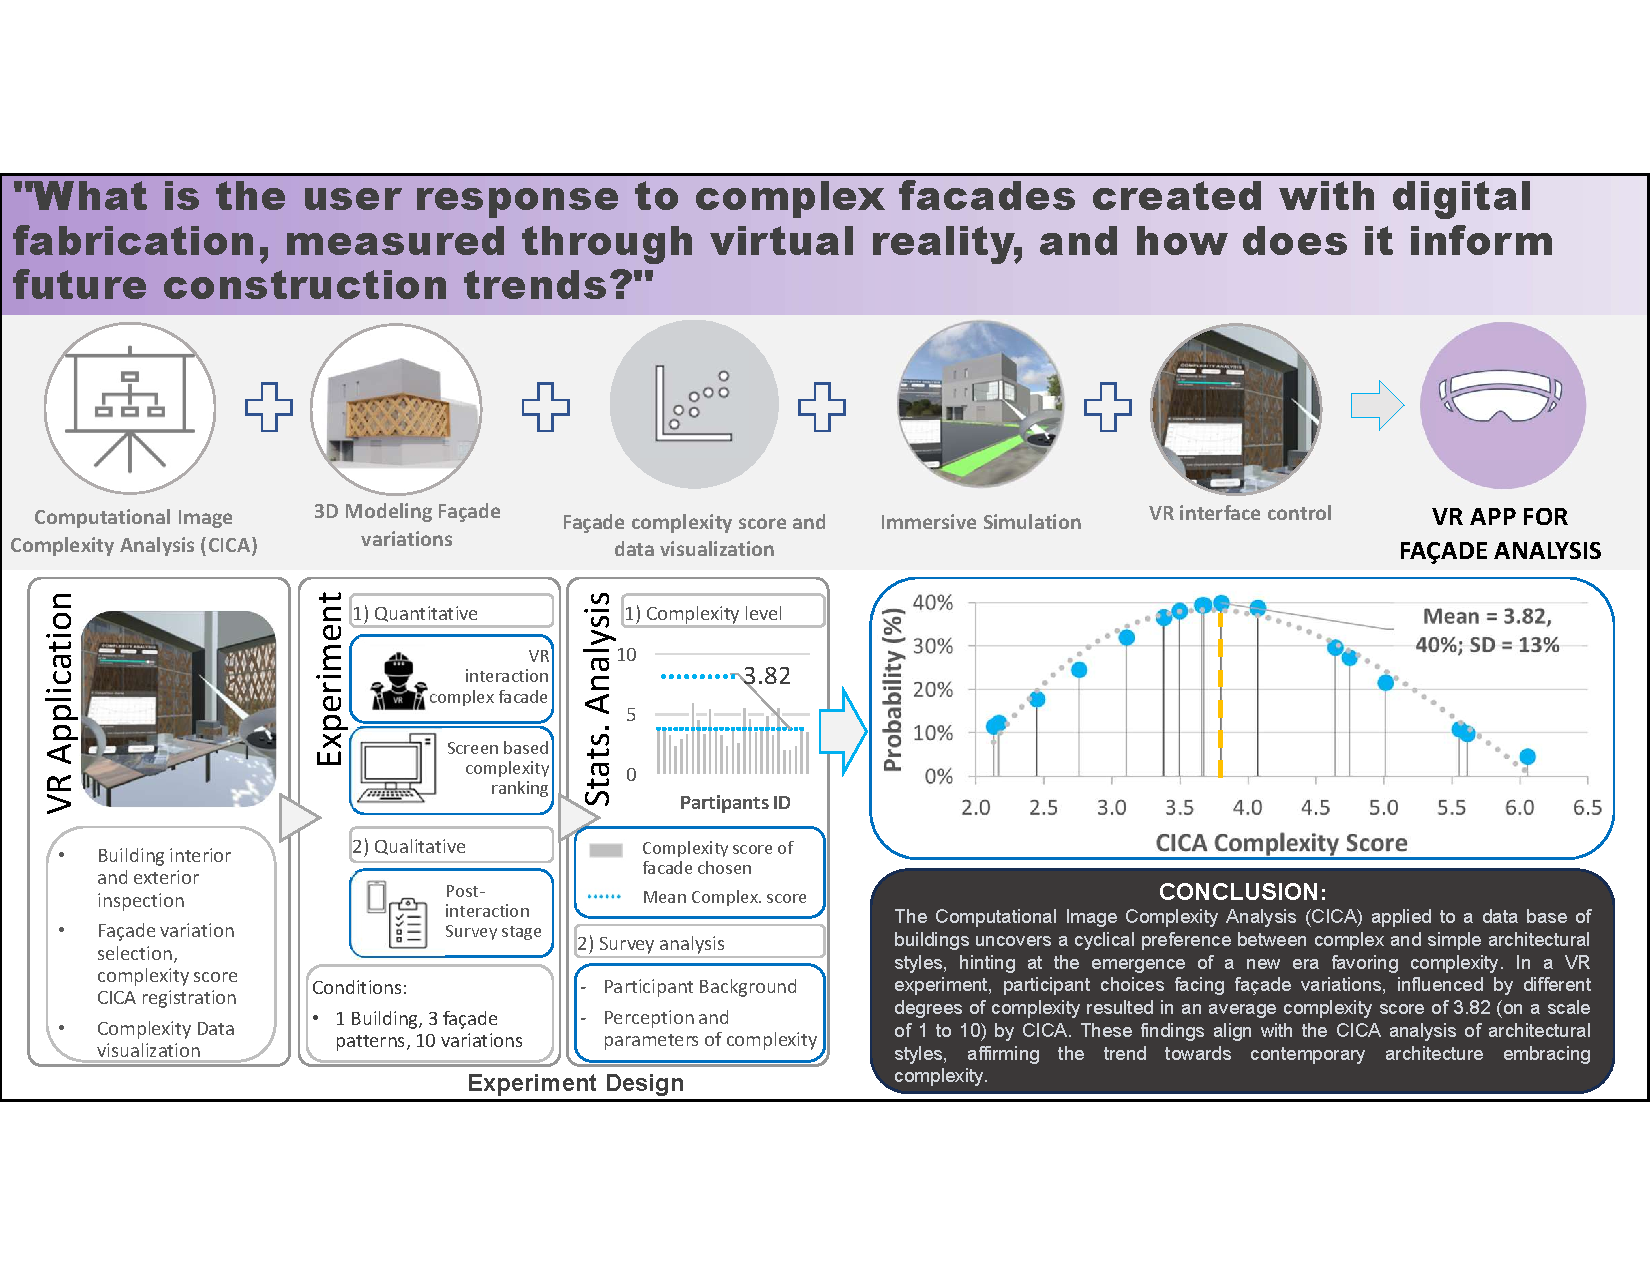
\includegraphics[width= \textwidth, trim = 0 80 0 80, clip]{Images/GraphicAbstract}
    \label{fig:graphic_abstract}
\end{graphicalabstract}

%%Research highlights
\begin{highlights}
%highlights

\item Computational Image Complexity Analysis (CICA) system using computer vision.
\item CICA system quantifies facade complexity, aiding in historical trend analysis.
\item VR experiment indicates user preference for moderate complexity in facades.
\item Future architecture favoring user-centric, complexity balanced designs trends.

\end{highlights}

\begin{keyword}
%% keywords here, in the form: keyword \sep keyword
Facade Design\sep Architectural Complexity\sep Virtual Reality\sep Computer Vision\sep Architectural Aesthetics \deleted{Data-Driven Design}

\end{keyword}

\end{frontmatter}
%\linenumbers
%\modulolinenumbers[10]
%
%! Main body of manuscript on separate file
%\linenumbers
%\modulolinenumbers[10]
%
\begin{linenumbers}

\section{Introduction}
\label{sec:1Introduction}
%%State the objectives of the work and provide an adequate background, avoiding a detailed literature survey or a summary of the results.
%%Introduction

%=================================
%%Reference
%%https://www.scribbr.com/research-paper/research-paper-introduction/
%%State the objectives of the work and provide an adequate background, avoiding a detailed literature survey or a summary of the results.

%Step1. Introduce your topic.
     %This is generally accomplished with a strong opening hook.
%Step2. Describe the background.
     %For a paper describing original research, you’ll instead provide an overview of the most relevant research that has already been conducted.
%Step3. Establish your research problem.
     %In an empirical research paper, try to lead into the problem on the basis of your discussion of the literature.
%Step4. Specify your objective(s).
     %The research question is the question you want to answer in an empirical research paper. If your research involved testing hypotheses, these should be stated along with your research question.
%Step 5: Map out your paper.
     %The final part of the introduction is often dedicated to a brief overview of the rest of the paper.

%recommended limit 500 words
%=================================

Recent advancements in Building Information Modeling (BIM) and digital fabrication are transforming architectural practice.
These technologies enable architects to design intricate and complex forms, moving beyond the uniformity of barren walls and fully glazed facades that often dominate contemporary streetscapes.
By leveraging these advancements, architects can introduce complexity and detail into their designs, enhancing both the visual and functional aspects of buildings, and creating more engaging and dynamic environments that potentially redefine the relationship between form and function~\cite{Leach2016}.

However, the pursuit of complexity in architectural design must be balanced with sustainability and user satisfaction.
Designs that are overly complex without consideration of these factors can quickly become outdated and disconnected from their inhabitants, leading to issues of obsolescence and lack of relevance~\cite{Oberfrancova2021}.
Understanding how complexity can enhance both environmental sustainability and user satisfaction is therefore crucial for modern architectural practice.

Previous research has extensively explored the impact of complexity in architectural design, identifying mathematical relationships between complexity and aesthetic value ~\cite{Bies2016, Douchova2016, Redies2015}.
Despite these insights, the architectural field has yet to develop frameworks that leverage these principles for practical design applications, especially considering modern technological advancements aimed at sustainability.

This study aims to bridge the gap between theoretical understanding and practical application by developing a methodology to measure facade complexity.
The objectives are to generate data that can improve `Data-driven Building Design' (DBD) by integrating a complexity scoring function that can inform on the optimal rate between simplicity and complexity based on historical analysis and user preferences.
By integrating complexity insights with modern technological applications, we seek to provide actionable, DBD insights for future architectural practices promoting the advancement aimed at sustainability.

The methodology is structured around 4 primary components:

\begin{enumerate}
    \item Literature review: Significant studies on the foundational theories of complexity, and an exploration of the fluctuation between simplicity and complexity in architectural history.
    \item Complexity Analysis System Development: Implements a Virtual Reality (VR) framework, and combines it with a Computational Image Complexity Analysis (CICA) component using computer vision (CV) algorithms to quantitatively assess the complexity of facade designs.
    \item Experiment Execution: involving VR to facilitate participant interaction with complex facades, augmented by surveys and interviews for qualitative insight.
    \item Data Analysis and Validation: Assessing the data collected during the experiment to evaluate the effectiveness of the Complexity Analysis System and CICA framework in measuring complexity and user preferences.
\end{enumerate}

\deleted{This comprehensive approach aims to enrich our understanding of facade complexity and its role in the contemporary Architectural, Engineering, and Construction (AEC) industry.}

This comprehensive approach aims to enrich our understanding of facade complexity and its role in the contemporary Architectural, Engineering, and Construction (AEC) industry.

\added{Comment 1: The author emphasized the importance of integrating sustainability and user satisfaction into facade design. However, how this study addresses sustainability concerns is not explicitly stated. Therefore, please provide further clarification on this aspect.}



%
%!Notes
Beauty is too difficult to translate into number so why bother?
Is beauty really subjective?
Why would we care? there is an

A 2011 survey in the United States found the strongest correlation between a place's physical beauty, and peoples satisfaction out of any other attributes!

Design disconnect. Architects and the public each seem to like different kinds of buildings. This effect was discovered by psychologist David Halpern. Study in 1987.

Beauty is nature way of

According to Denis Dutton, all things that we find beautiful have three things in common: Firstly: they have a shape or characteristics we inherently like.
Secondly, they are fit for their purpose.
And thirdly, they are well-made and display skill in their making.

Organised complexity. As humans, we seem to need some complexity or diversity of form but not too much. Only order is boring, but only complexity is chaos. We seem to like things that are somewhere in the middle. A plain facade too ordered, so we ignore it. A facade like this on the other hand is too

Evidence based design

%!Sustainability
%cause gimmicks, like fashion, get outdated at some point. Many buildings built in the last 50 years already need to be torn down, as they did not have the qualities that made people connect to them. All this renovating and rebuilding requires massive amounts of new concrete, glass and steel. All at a huge cost for society. And, of course, for the environment.


%!Thesis
%we link fractals and organized complexity to environmental optimization to combine them in a theory od data driven beauty environental design. We established that the complexity theory and the vr influence as representative of MR tehconologies serves to built on the aspect of creating a paneling system with organized complexity since it has proven that beauty is perceived by it and we guarantee to add value and improtance to cities based on the papers and video "What makes a building beuatiful".
%!Video article

Architecture:\cite{Aesthetic2022}



Organise your facade in a clear, readable way, so people can make sense of how load bearing features connect to each other
Apply some form of ornament to connect separate parts of the building and to offer the fractal & symmetrical qualities people subconsciously connect to
Prevent the creation of large blank walls or glass facades at eye level. Glass is hard to ‘read’ – people can’t focus their eyes well on it as it is partly reflective, partly translucent.
Apply (local) symmetry in your design. The building can be asymmetrical if building volumes on both sides of a central axis are ‘balanced’
Richly detail the facade if possible, with details on various levels of scale, or utilise materials with some pattern to offer fractal qualities in the surface
Build according to local preferences, history, culture – study the ‘Genius Loci’.
Use curves in your design wherever possible
Urbanism:

Utilise street trees wherever possible
Apply ‘gentle density’: “In contrast to high density, which includes mid- and high-rise residential buildings, gentle density refers to development of duplexes, triplexes, accessory dwelling units (ADUs), stacked townhouses, semi-detached homes and small-scale apartment and condominium buildings within and among single-family zoned neighborhoods. Gentle density promotes mixed-use development, with single-family homes alongside small multi-family homes, businesses and commercial buildings. Gentle density aims to retain neighborhoods’ residential identity and feel while alleviating housing crises.”

modern brain imaging methods have empowered studies on how aesthetic experience
correlates with the activation of brain regions in the human
observer and advanced computational methods permit the investigation of statistical
image properties that are associated with aesthetically pleasing images\cite{Redies2015}

Despite the uncertainties, there seems to be a general agreement in the field that the scien-tific study of aesthetic experience and of beautiful stimuli holds
great promise and may contribute significantly to our under-
standing of human brain function and behavior\cite{Redies2015}

Birkhoff (1933)\cite{Birkhoff1933} first formalized aesthetic value as the ratio of order and complexity.
Complexity, to Birkhoff (1933), was a
physical, measurable characteristic that could be described
mathematically \cite{Bies2016}

Birkhoff\cite{Birkhoff1933} defines an aesthetic measure and applies it to several types of objects with different modes of perception – visual, including
3D objects, and auditory (music, poetry).
The measure is defined in relation to the effort which the object demands of the perceiver (complexity), and the pleasing or displeasing features which can be recognised in the object (order).\cite{Douchova2016}
%!aesthetics

Recent experimental studies began examining the neuroaesthetics of the built envi-
ronment [166–170]. But most offer a perspective almost completely limited to modernist
aesthetics and fail to consider traditional design let alone the fractal mathematics of per-
ception [3,171–180]. \cite{Brielmann2022}

%!Complexity

Complexity & Order is rich sensory information that adheres to a spatial hierarchy similar to those encountered in nature. \cite{Browning2014}

A space with good Complexity & Order feels engaging and information-rich, as an intriguing balance between boring and overwhelming.\cite{Browning2014}

The Complexity & Order pattern has evolved from research on fractal geometries and preferred views; the perceptual and physiological responses to the complexity of fractals in nature, art and architecture; and the predictability of the occurrence of design flows and patterns in nature.\cite{Browning2014}




Researches have found that
The consistency of natural themes in historic structures and places suggests that
biophilic design is not a new phenomenon; rather, as a field of applied science,
it is the codification of history, human intuition and neural sciences showing that
connections with nature are vital to maintaining a healthful and vibrant existence
as an urban species.\cite{Browning2014}

Fractals are patterns that repeat at increasingly fine sizes and so create shapes of rich visual complexity.
Prevalent in nature, clouds, trees, and mountains are common examples, as are cauliflowers and fern leaves.
This paper dives into the complex minutiae of vision and fractals, and how they can place the observer in the “comfort zone”.\cite{Browning2014}

Richly detail the facade if possible, with details on various levels of scale, or utilise materials with some pattern to offer fractal qualities in the surface\cite{Aesthetic2022}

Complexity & Order is rich sensory information that adheres to a spatial hierarchy similar to those encountered in nature. \cite{Browning2014}

A space with good Complexity & Order feels engaging and information-rich, as an intriguing balance between boring and overwhelming.\cite{Browning2014}

The Complexity & Order pattern has evolved from research on fractal geometries and preferred views; the perceptual and physiological responses to the complexity of fractals in nature, art and architecture; and the predictability of the occurrence of design flows and patterns in nature.\cite{Browning2014}

Birkhoff (1933)\cite{Birkhoff1933} first formalized aesthetic value as the ratio of order and complexity.
Complexity, to Birkhoff (1933), was a
physical, measurable characteristic that could be described
mathematically \cite{Bies2016}

Birkhoff\cite{Birkhoff1933} defines an aesthetic measure and applies it to several types of objects with different modes of perception – visual, including
3D objects, and auditory (music, poetry).
The measure is defined in relation to the effort which the object demands of the perceiver (complexity), and the pleasing or displeasing features which can be recognised in the object (order).\cite{Douchova2016}




Traditional architecture knew how to explore \cite{Browning2014}



Despite extensive research in data-driven building design aimed at optimizing resource use and environmental sustainability, many buildings still fail to resonate with the people who inhabit them, leading to premature demolition.
Computational advancements have the potential to transform urban landscapes; however, without addressing the psychological connection between people and their built environment, even sustainably designed buildings may suffer the same fate as their predecessors, cause fashion-like gimmicks become obsolete over time, leading to significant societal and environmental costs\cite{Aesthetic2022}.
Beauty significantly contributes to emotional attachment and happiness in urban areas\cite{Brielmann2022}, yet beauty is largely considered as subjective and relinquished to aesthetic ideologies generating short-fashion urban fabric, however neuroscientists and anthropologists have found certain universal preferences organized in built structures on neurophysiological criteria and measurements that allow to circunvent old and inconclusive debates in aesthetics and architectural history\cite{Brielmann2022}.

Citations by brielmann 2022

The data reviewed here show that we fundamentally need to change how we design
the built environment.
It is time for people to place urban well-being above aesthetic ideology; the durability and long-term reusability of urban fabric above fashion. Changing
built environments—from “old-fashioned” to new, slick, and shiny—is a huge mistake, as people all over the world realize that we need emotional nourishment from the environment around us.
“Old-fashioned” surroundings could likely contain essential healing qualities.
We deserve to walk down a street that is beautiful, as judged by our biology, not by
some imposed stylistic criterion.
We deserve to be protected from the negative psychological reactions caused by experiencing neuroaesthetically inappropriate if not harmful design.
Based on our latest scientific understanding of perception, we need to reclaim
the appropriate and practical design toolkits of past generations to accomplish these ends.
Only then will we be able to build places for the greatest well-being of the greatest number of users.


Yet a new issue arises while extensive research in data-driven building design has been done in pursuit of optimization of resources and environmental engineering, buildings continue to fall out of grace and being demolished by failing to connect with the people that inhabit them.
The computational advancements provide the chance to transform the city scape however if no attention is directed to bring about that attachment with people regardless of it sustainability these new buildings will follow the same lifespan as their predecessors, cause gimmicks like fashion, get outdated at some point All at a huge cost for society. And, of course, for the environment. \cite{Brielmann2022}



%!%Figures of timelines
    % Old, middle and contemporary timeline
    \begin{table*}[htb]
        \centering
        \small
        \begin{tabular}{c}
            %Top cell with one figure
            %Figure early timeline
            \begin{minipage}{\textwidth}
                \centering
                \includegraphics[width= \linewidth]{Images/OldTimeline}
                        \captionof{figure}{Early timeline. Sequential representation of architectural styles illustrating the shift between complexity and simplicity. From left to right: Romanesque[a] with its solid and massive structure; Gothic[b] featuring verticality and lightness; Classicism[c] characterized by geometrical clarity and order; Baroque[d] with dynamic shapes and rich decorations; followed by the restrained and symmetrical formality of Neo-classicism[e]. (\textit{Images edited from source})}
                        \label{fig:Oldtimeline}
            \end{minipage}
            \\
            %Middle cell
            %Middle timeline
            \begin{minipage}{\textwidth}
                \centering
                \includegraphics[width= \linewidth]{Images/MiddleTimeline}
                        \captionof{figure}{Transitional timeline. Sequential representation of architectural styles illustrating the shift between complexity and simplicity. From left to right: Art Nouveau[a] with its fluid lines and natural forms; Art Deco[b], marked by bold geometry and opulence; Modernism's[c] pursuit of stripped-back functionality; culminating in Postmodernism's[d] revival of historical styles and complexity (\textit{Images edited from source})}
                        \label{fig:Middletimeline}
            \end{minipage}
            \\
            %bottom Cell
            %Contemporary timeline
            \begin{minipage}{\textwidth}
                \centering
                \includegraphics[width= \linewidth]{Images/contemporaryTimeline}
                        \captionof{figure}{Contemporary timeline. Sequential representation of architectural styles illustrating the shift between complexity and simplicity. Era of exploration and innovation. From left to right: Deconstructivism[a], characterized by fragmentation and non-linear design; Neofuturism[b], capturing movement and technology-infused aesthetics; High-tech modernism[c], focusing on visible structural elements and technological expression; Parametricism[d], with its algorithm-based complex forms; and Pragmatic utopianism[e], blending idealistic designs with practical applications (\textit{Images edited from source})}
                        \label{fig:contemporarytimeline}
            \end{minipage}
        \end{tabular}
    \end{table*}


\section{Literature review}
\label{sec:LiteratureReview}
%% Research Background

%% A Theory section should extend, not repeat, the background to the article already dealt with in the Introduction and lay the foundation for further work. In contrast, a Calculation section represents a practical development from a theoretical basis.

%A theoretical framework is a foundational review of existing theories that serves as a roadmap for developing the arguments you will use in your own work.

%=============================================================================
%Outline.
%1. Introduction
%2. The importance of facade in a building.
%3. A brief analysis of architecture styles and the shift from Images and simplicity
%3. A reflexion into digital fabrication techniques specially parametric design.
%4. The principle of data driven design.
%5. An analysis into mixed reality and the advantages of introducing this  into the design review.
%=============================================================================

%///////////////////////////////////////////////////////////////
%% refined outline of theory framework

%% Introduction

%!Concise intro

This section explores the multi-faceted nature of architectural complexity, from its historical evolution to contemporary technological advancements.
It aims to provide a comprehensive understanding of how complexity influences both design practices and user experiences.

This section focuses on four key themes:
\begin{itemize}
    \item Evolution and Theoretical Foundations of Architectural Complexity: Explores the historical context and foundational theories of complexity in architecture, including Birkhoff's ratio of order to complexity.
    \item Technological Advancements: Analyzes the impact of BIM, digital fabrication, and VR on architectural design and user perception.
    \item User Perception and Quantitative Analysis of Complexity: Investigates the psychological and physiological impacts of complexity on users, principles of biophilic design, and gaps in aligning data-driven design with user satisfaction.
    This includes quantitative methods and computational studies on complexity.
    \item Gaps in Current Research: Identifies the existing gaps in the research, highlighting the need for comprehensive frameworks that integrate theoretical principles with practical applications, and discusses the challenges and opportunities of rapidly advancing technologies.
\end{itemize}

These insights will be instrumental for validating CICA findings by comparing empirical data with theoretical insights into architectural evolution, confirming observed patterns of simplicity and complexity.






    %\subsection{Studies on aesthetic preferences related to compexity}
%\label{subsec:TimelineArchitectureStyles}

%--------
%Evolution and Theoretical Foundations of Architectural Complexity
%Introduction to Complexity in Architectural Design
%Historical Context: Discuss the evolution of architectural complexity from classical architecture to modernist minimalism and contemporary design.
%Theoretical Foundations: Explore foundational theories and concepts, such as Birkhoff's ratio of order to complexity \cite{Birkhoff1933}.Evolution and Theoretical Foundations of Architectural Complexity
%--------

%Evolution and Theoretical Foundations of Architectural Complexity

Historical Context


Architecture stands as a unique art form, transforming the ordinary into the extraordinary while fulfilling functional purposes \cite{Hnin2022}.
Its evolution is marked by a dynamic interplay between simplicity and complexity, reflecting societal values and technological advancements \cite{Economakis2023}.
From early architectural styles like Romanesque, characterized by robust and simplistic forms, to the Gothic period with its intricate, skyward designs \cite{Stacbond2020}, architecture has oscillated between simplicity and complexity (see Figure \ref{fig:Oldtimeline} a,b).

The Renaissance heralded a revival of Greek and Roman ideals with a focus on symmetry, followed by the Baroque's lavish ornamentation in the 16th century \cite{Economakis2023} (see Figure \ref{fig:Oldtimeline} c,d).
The Neoclassical style, dominant in the 18th and 19th centuries, emphasized symmetry and classical principles while integrating new technologies like reinforced concrete \cite{Economakis2023} (see Figure \ref{fig:Oldtimeline} e).
Art Nouveau and Art Deco, emerging in the late 19th and early 20th centuries, celebrated nature and technological advancements, marking a departure from Neoclassical restraint \cite{Salas2018, Arora2023} (see Figure \ref{fig:Middletimeline} a, b).

The 20th century saw the rise of Modern Architecture, which advocated for "form follows function" and minimal ornamentation, a significant departure from previous ornate designs \cite{Gage2015}.
Figures like Adolf Loos and Le Corbusier championed minimalism and functionality, influencing a generation of architects to prioritize structural honesty and simplicity \cite{Saglam2014}.
However, this movement often led to uniform urban landscapes that lacked the cultural richness and diversity of their predecessors (see Figure \ref{fig:Middletimeline} c).

In response to Modernism's perceived limitations, the late 1960s saw the emergence of Postmodernism, spearheaded by thinkers like Robert Venturi.
Postmodernism critiqued the minimalist aesthetic and reintroduced complexity, ornament, and form into architectural design, advocating for buildings that engage more deeply with their cultural and historical contexts \cite{Venturi1972} (see Figure \ref{fig:Middletimeline} d).

The late 20th and early 21st centuries have seen a resurgence in creativity and expression, with architects utilizing digital technologies to explore new realms of complexity and ornamentation \cite{Burlando2019} (see Figure \ref{fig:contemporarytimeline}).
The fusion of digital and physical design processes signals a shift towards the democratization of complex, parametric designs, indicative of a contemporary period that values ornamentation, functionality, and human comfort \cite{Schwab2016}.
This evolving trajectory of architecture suggests a future where design is deeply intertwined with societal values and technological possibilities.

Facades and ornamentation, in this context, become critical in conveying these narratives, bridging the gap between the aesthetic and the symbolic, and establishing the interface between buildings and their environments, influencing comfort and energy efficiency while reflecting the building's identity \cite{Kamal2020}.
The evolution of facade design and ornamentation mirrors societal transformations, technological progress, and shifts in artistic sensibilities, each impacting how communities relate to their built environment.

In conclusion, the historical context of architectural complexity reveals a rich tapestry of styles and philosophies, from ancient grandiosity to modern minimalism and contemporary innovation.
These shifts reflect the ongoing dialogue between simplicity and complexity, tradition and innovation, and functionality and aesthetics, shaping the built environment in ways that are both imaginative and responsive to societal needs.

Theoretical Foundations

Contemporary architecture, however, has seen a resurgence of interest in complexity, driven by advancements in Building Information Modeling (BIM) and digital fabrication. These technologies have allowed architects to explore forms and structures that were previously impractical or impossible to realize. The renewed focus on complexity reflects a broader understanding that architectural design can and should engage with both functional requirements and aesthetic aspirations, offering environments that are visually stimulating and experientially rich \cite{Gage2015}.

One of the foundational theoretical contributions to understanding architectural complexity is George David Birkhoff's theory of aesthetic measure, introduced in 1933. Birkhoff proposed that aesthetic value could be quantified through a ratio of order to complexity. His formula, M = O/C (where M is the aesthetic measure, O is order, and C is complexity), suggests that the most aesthetically pleasing designs achieve a balance between these two elements \cite{Birkhoff1933}. This theory provided a framework for evaluating the aesthetic appeal of architectural forms based on their structural and decorative elements.

Birkhoff's ideas have influenced subsequent research on architectural complexity, encouraging a systematic approach to studying how different design elements contribute to the overall aesthetic experience. This balance between order and complexity is central to contemporary efforts to integrate complexity into architectural design in a way that enhances both user satisfaction and sustainability.

Another significant theoretical framework is Christopher Alexander's concept of "pattern language," introduced in the 1970s. Alexander's work emphasized the importance of recurring design patterns that resonate with human users on a fundamental level. His theory suggests that certain patterns, when combined effectively, can create environments that feel harmonious and alive. This approach aligns with the principles of biophilic design, which seeks to connect architecture with natural elements to enhance human well-being.

Contemporary research continues to build on these theoretical foundations, exploring how advanced technologies can be used to create complex designs that are both aesthetically pleasing and functionally effective. The integration of digital tools such as BIM and computational design methods has enabled architects to push the boundaries of complexity, creating structures that are not only visually striking but also optimized for performance and sustainability.

In summary, the evolution of architectural complexity is a testament to the ongoing interplay between cultural, technological, and theoretical influences. From ancient grandiosity to modern minimalism and contemporary innovation, architects have continually sought to balance order and complexity to create meaningful and engaging built environments. Theoretical frameworks such as Birkhoff's aesthetic measure and Alexander's pattern language provide valuable insights into how complexity can be harnessed to enhance architectural design, offering a foundation for future explorations in this dynamic field.


%However, the indiscriminate pursuit of popular trends using new technologies can lead to designs that quickly become outdated.
%Fashion-like gimmicks, often adopted without a deeper understanding of their long-term impact, do not necessarily resonate with users over time.
%Consequently, many buildings constructed in the last fifty years are now facing demolition, lacking enduring qualities that foster a genuine connection with their inhabitants \cite{Aesthetic2022}.
%This highlights a critical need for architectural practices that not only embrace innovation but also ensure relevance and sustainability through designs that engage and inspire \cite{Brielmann2022}.
%
%Despite significant research aimed at optimizing resource use and boosting environmental sustainability, the disconnect between data-driven design and user satisfaction remains pronounced.
%While computational advancements hold potential to transform urban landscapes, neglecting the psychological connection between people and their built environment can doom even sustainably designed buildings to obsolescence, incurring substantial societal and environmental costs \cite{Aesthetic2022}.
%Neuroscientists and other researchers have been working to define the aspects that stimulate our satisfaction with the built environment that transcend subjective aesthetic judgments, suggesting that certain structural elements resonate universally on a neurophysiological level, offering emotional nourishment and promoting urban well-being \cite{Brielmann2022}.
%These themes are often found in Biophilic design patterns that articulate the relationships between nature, human biology, and the design of the built environment.
%
%Historical and contemporary architectures have frequently incorporated natural patterns and complexities into their designs, underscoring a fundamental human affinity for biophilic elements that enhance psychological and physical well-being in urban environments.
%These design strategies, grounded in biophilic principles, align closely with the ingrained human need for interaction with nature-like settings, supporting a vibrant existence within urban landscapes \cite{Browning2014}.
%The recurring use of fractal geometries, seen in the repetitive patterns of elements like clouds, trees, and fern leaves, exemplifies nature's inherent complexity that has historically influenced architectural aesthetics.
%These natural complexities, when incorporated into building designs, place observers in a 'comfort zone' of sensory engagement, balancing stimulation and comfort through visually rich yet orderly environments \cite{Browning2014}.
%
%This well-established relationship between natural patterns and human well-being was mathematically formalized by Birkhoff (1933), who introduced a ratio of order to complexity as a measure of aesthetic value \cite{Birkhoff1933}.
%Despite some uncertainties, there is a widely held consensus within the field that exploring the scientific dimensions of aesthetics and appealing stimuli can offer profound insights into human brain functionality and behavior, significantly enriching our comprehension of these processes \cite{Redies2015}.
%This belief supports the quantitative frameworks established by Birkhoff in 1933, which assess and integrate complexity into design, emphasizing a balanced and engaging complexity as essential for effective architectural expression \cite{Birkhoff1933}.
%Despite these insights, the architectural field has not fully developed a framework that allows us to leverage these principles in complexity analysis.
%Although many tools exist for environmental optimization of buildings, there is still a gap in establishing a balance between complexity and order.
%This research seeks to bridge this gap by incorporating a methodology for measuring the complexity outputted during the design phase of building facade design, generating quantifiable data on the order of complexity of iterations of facade design that can be used to improve data-driven optimization models for building design.

    %\subsection{The Architectural Journey: Oscillations Between Simplicity and Complexity}
    %\label{subsec:TimelineArchitectureStyles}
    %
%\subsection{Human-Centric Design Philosophy across the history of architecture styles}
%\label{subsec:TimelineArchitectureStyles}

%===========================
%%Human-Centric Design Philosophy: Explore the historical evolution of architectural philosophies that prioritize human experience and well-being. Discuss how different architectural styles and movements have addressed the balance between ornamentation, functionality, and human comfort.
%===========================
%!Concise version

Architecture stands as a unique art form, setting itself apart from other creative mediums.
It requires not only the transformation of the ordinary into the extraordinary, akin to painting and sculpture, but also the imperative to fulfill the purpose and functionality of a building\cite{Hnin2022}.
Its evolution is marked by a dynamic interplay between simplicity and complexity, reflecting societal values and technological advancements\cite{Economakis2023}.
Historical shifts, from the Romanesque to Gothic styles, exemplify this oscillation, as seen in the transition from robust, simplistic forms to intricate, skyward designs\cite{Arora2023, Stacbond2020} (see Figure\ref{fig:Oldtimeline} a,b).

The Renaissance heralded a revival of Greek and Roman ideals and the return to symmetry, that is succeeded by the Baroque's lavish ornamentation in the 16th century\cite{Economakis2023} (see Figure\ref{fig:Oldtimeline} c,d).
The Neoclassical style, with its emphasis on symmetry and classical principles, dominated the 18th and 19th centuries, integrating new technologies like reinforced concrete\cite{Economakis2023}(see Figure\ref{fig:Oldtimeline} e).
However, its rigid academicism eventually led to more ostentatious designs, setting the stage for the emergence of Art Nouveau and Art Deco (see Figure\ref{fig:Middletimeline} a, b).
These styles, celebrating nature and technological advancements, marked a departure from Neoclassical restraint\cite{Salas2018, Arora2023}.

The 20th century saw the rise of Modern Architecture, advocating `form follows function' and minimal ornamentation, a reaction against previous excesses\cite{Gage2015, Venturi1972} (see Figure\ref{fig:Middletimeline} c).
Postmodernism, emerging in the late 1960s, challenged this minimalism, reintroducing ornament and form into architectural design.
The late 20th century witnessed a resurgence of expression and imagination, with architects leveraging digital technologies to create complex, ornate structures\cite{Burlando2019} (see Figure\ref{fig:Middletimeline} d).

Now, at the dawn of the 21st century, the convergence of digital and physical realms forecasts a democratization of complex, parametric designs, signaling a contemporary era embracing complexity and ornament\cite{Schwab2016}.
This trajectory suggests a future where architecture harmonizes ornamentation, functionality, and human comfort, resonating with current values and technological capabilities.

%!Previous human centric design philosophy

%Architecture stands as a unique art form, setting itself apart from other creative mediums.
%It requires not only the transformation of the ordinary into the extraordinary, akin to painting and sculpture, but also the imperative to fulfill the purpose and functionality of a building\cite{Hnin2022}.
%
%At the core of architectural evolution resides a dynamic interplay between simplicity and complexity, often guided by the intersection of societal values and technological advancements\cite{Economakis2023}.
%However, it's important to clarify that within the context of this research, neither simplicity nor complexity carry any inherent negative or positive connotations.
%Using the term ``simplicity`` here doesn't imply a condemnation of one style in favor of another;
%rather, it highlights that throughout the history of architecture and its various styles, there have been periods characterized by evident complexities as well as phases where designs embraced apparent simplicities that hid their intricacies into themselves.
%Undoubtedly, every prevailing architectural style of its time has contributed masterpieces to the built environment.
%
%Consider, for instance, the transition from the robust Romanesque classic style of the 10th century, notably exhibited in churches, to the Gothic style brought by groundbreaking advancements of the 12th century that introduced buttresses, revolutionizing load distribution\cite{Arora2023}(see Figure\ref{fig:RomanesquevsGothic}).
%This innovation propelled churches skyward, inviting luminous interplays to embellish the interiors through stunning stained-glass windows bedecked in intricate design\cite{Stacbond2020}.
%
%This oscillation between complexity and simplicity persists through time— transitioning from the intricate Gothic style to the revival of Greek and Roman ideals, exemplified by the symmetrical perfection of the Renaissance era in the 14th century.
%
%This resurgence was succeeded by the opulent ornamentation and exuberance of the Baroque style in the 16th century, essentially a creation of the Chatolic church, that started in Europe and later spread across the New world in other Chatolic nations.
%It was characterized by the preference for curves over the straight line, an interest in complex plans and volumes, overlapping architectural forms, and an interest for combining the three arts of painting, sculpture and architecture\cite{Economakis2023}.
%
%The progression continued with the classical revival of the 18th century, heavily influenced by the architectural principles of classical Greece and the Palladian style.
%This revival aimed to create picturesque compositions and sought to reestablish the rational simplicity that defined ancient Greece and Rome\cite{Economakis2023}.
%
%The late 18th century marked the beginning of globalization and an information explosion, which enabled scientific advancements but also blurred the geographical origins of architectural forms.
%As a result, architectural expressions from diverse cultures became acceptable options in various contexts.
%This phenomenon led to the incorporation of multiple historical references into buildings, soon Gothic, Oriental or even Egyptian styles, to name a few, were integrated into victorian houses, resulting in stylistic confusion known as Relativism and Subjectivism.
%Architects grappled with a multitude of options and no clear consensus on architectural expression\cite{Economakis2023}.
%
%In response to this architectural chaos, the Neoclassical style would appear, envisioned under the conservative academicism of the 19th century that aimed to bring order by consolidating the architectural profession under the teachings of classical architecture as idealized during the Renaissance.
%Characterized by being bilaterally symmetrical and sel-referential or a-contextual with little regard to how they integrated to urban settings.
%This heavily inspired greek and Palladian architecture would integrate with new technologies like reinforced concrete and cast iron.
%Led by the École des Beaux-Arts in Paris, the Neoclassic style gained prominence and persisted until the early 20th century\cite{Economakis2023}.
%
%However, by the late 19th century, the increasingly rigid academicism of the École des Beaux-Arts gave way to a shift towards ostentation.
%The lack of volumetric hierarchy in building designs led to a departure from the sobriety and principles of the Renaissance.
%Their monumentality originally praised was now resulting in a tendency towards overelaboration as buildings competed for attention\cite{Economakis2023}.
%
%In the late 19th century, amidst the prevalent Neoclassical style, two influential design movements emerged: Art Nouveau and Art Deco.
%
%The Art Nouveau movement, which thrived from 1890 to 1910, celebrated nature and found its essence in organic forms.
%It was characterized by intricate and fluid designs, embracing curvilinear motifs and intricate ornamentation.
%
%Antonio Carlos Gaudí, a figure of unparalleled renown within this movement, not only exemplified the Art Nouveau style but also exhibited distinctive elements that set his work apart and positioned him ahead of his time.
%Gaudí's architectural genius extended beyond aesthetics, pioneering concepts such as sustainability and biomimetic architecture, long before these ideas took hold in architectural discourse\cite{Salas2018}(Figure\ref{fig:ArtNouveauVsModernism}).
%
%The subsequent Art Deco movement, flourishing during the 1920s and 30s, celebrated technological advancement through luxurious materials and intricate patterns.
%It blended modern design with artistic craftsmanship, embracing geometric shapes, bold colors, and streamlined forms.
%Art Deco architecture often featured sleek lines, zigzags, and stylized motifs, capturing the spirit of the era's dynamism and opulence\cite{Arora2023}.
%
%These innovative styles of the late 19th century, while revolutionary in their own right, seemed to herald an impending era of transformation.
%While not as universally embraced as the Neo-Classical style, which held sway in the 19th century, these styles indicated a shift in the broader attitude towards the teachings of the Ecole des Beaux Arts and its penchant for exuberance and monumentality.
%
%Nonetheless, the friction against the teachings of the Ecole des Beaux Arts and its reverence for exuberance reached its zenith as the 20th century unfolded.
%
%Especially prominent among architects with a more socially-minded inclination, this antagonism would pave the way for the emergence of Modern Architecture and rationalism during the first half of the 20th century.
%
%These movements brought about radical shifts in architectural paradigms, shaking the very foundations of conventional design (see Figure\ref{fig:NeoclassicalvsModernism}).
%
%%%Figure neoclassicim vs modernism
%     \begin{figure}[htb]
%          \centering
%          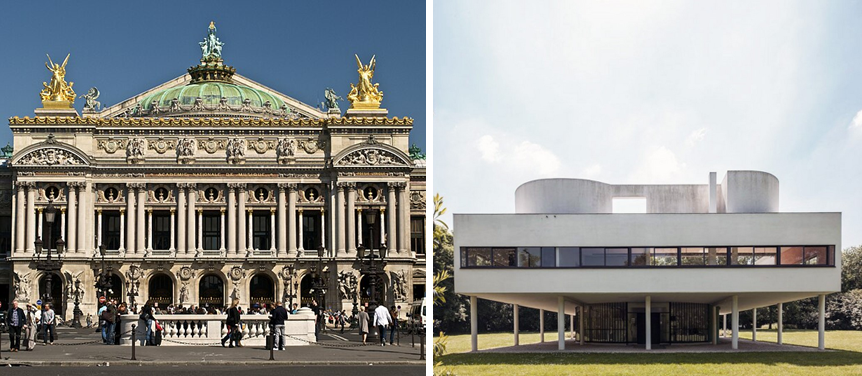
\includegraphics[width= \linewidth]{Images/NeoclassicismVsModernism}
%          \caption{Neoclassic building "Paris Opera" 19th AC (left) vs Modernist house "Villa Savoye" 20th AC (right). From Complexity to simplicity. (\textit{Images edited from source:\cite{Stacbond2020}})}
%          \label{fig:NeoclassicalvsModernism}
%        \end{figure}
%
%This architectural ethos adopted the maxim ``Form follows function'', emphasizing functionalism and characterized by a rejection of traditional ornament in favor of new forms of more subtles intricacies like the “aesthetics of machinery” that showcased architecture  enriched  with  only  the  beauty of its lines and the use of new-age materials such as steel, glass, and concrete\cite{Gage2015}.
%
%Venturi et al.\cite{Venturi1972} delve deeper into the reflections on modern architecture, which was often regarded as progressive, if not revolutionary, as well as utopian and puristic.
%They elucidate how architects of this movement, when confronted with dissatisfaction towards existing conditions, often leaned towards tearing down and rebuilding, rather than seeking to enhance or adapt what already existed.
%
%This tendency for radical transformation rather than gradual evolution underscores the assertive and sometimes uncompromising nature of modernist architectural interventions.
%
%%% add some extra references to the modernist section specially about the urban configuration
%
%The postmodernism style of the late 60's marks a radical return of ornament in form recognizing that even simplified modern elements serve as ornamentation focusing on the thought of freeing design element from oppresive modern constraints.
%
%
%
%The late 20th century embraced imagination and expression through architects like Frank Gehry, Zaha Hadid, and Rem Koolhaas.
%Their constructions stood as monumental expressions of ornament, enabled by digital technologies (Figure\ref{fig:Modernismvspostmodernism}).
%%
%%%Figure neoclassicim vs modernism
%     \begin{figure}[htb]
%          \centering
%          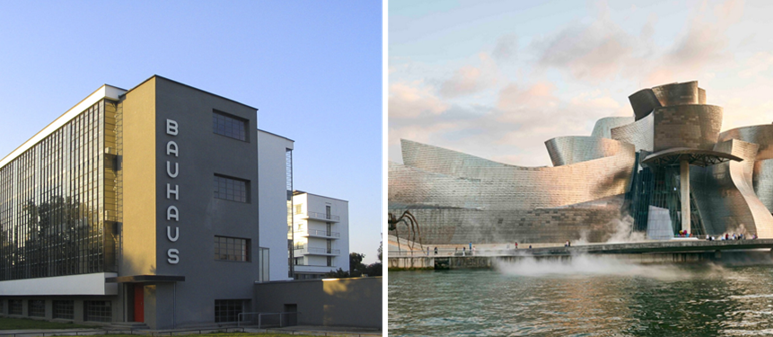
\includegraphics[width= \linewidth]{Images/modernism vs postmodernism}
%          \caption{Modernist building "Bauhaus School" 20th AC (left) vs Postmodernist "Guggenheim museum" 1997 (right). From simplicity to Complexity. (\textit{Images edited from source:\cite{Arora2023}})}
%          \label{fig:Modernismvspostmodernism}
%        \end{figure}
%
%Intricate shapes and structures have materialized, spanning from juxtaposed ornaments to innovative transformative structural ornamentation.
%This pursuit of complexity is a global phenomenon, prompting a competitive quest among leading contemporary architectural firms to harness parametric design as a tool to conceive groundbreaking new buildings.\cite{Burlando2019}.
%
%However, due to their complexity, these structures remained exceptional, not integrated into the urban fabric.
%Now at the beginning of the 21st century and the advent of the 4th industrial revolution, characterized by a fusion of technologies that is blurring the lines between the physical, digital, and biological spheres\cite{Schwab2016}, forecasts the democratization of digital fabrication which in turn will bring a paradigm shift, offering globally to all cultures the means to express authenticity through complex parametric designs, signaling a contemporary era embracing complexity and ornament.
%
%Amidst this historical exploration, it becomes evident that the architecture of the future is poised to harmonize ornamentation, functionality, and human comfort.
%The trajectory points towards a style of complexity—a style that crafts a delicate equilibrium, resonating with the values of our time and the technological possibilities at our fingertips.
%
%In this intricate interplay, architecture emerges as a tangible synthesis of human experience and creative expression, balancing ornament's aesthetic allure, the essential functionality of the built environment, and the crucial comfort of its inhabitants.


    %\subsection{Evolution and Theoretical Foundations of Architectural Complexity}
    %\label{subsec:ComplexityStudies}
    %%\subsection{Studies on aesthetic preferences related to compexity}
%\label{subsec:TimelineArchitectureStyles}

%--------
%Evolution and Theoretical Foundations of Architectural Complexity
%Introduction to Complexity in Architectural Design
%Historical Context: Discuss the evolution of architectural complexity from classical architecture to modernist minimalism and contemporary design.
%Theoretical Foundations: Explore foundational theories and concepts, such as Birkhoff's ratio of order to complexity \cite{Birkhoff1933}.Evolution and Theoretical Foundations of Architectural Complexity
%--------

%Evolution and Theoretical Foundations of Architectural Complexity

Historical Context


Architecture stands as a unique art form, transforming the ordinary into the extraordinary while fulfilling functional purposes \cite{Hnin2022}.
Its evolution is marked by a dynamic interplay between simplicity and complexity, reflecting societal values and technological advancements \cite{Economakis2023}.
From early architectural styles like Romanesque, characterized by robust and simplistic forms, to the Gothic period with its intricate, skyward designs \cite{Stacbond2020}, architecture has oscillated between simplicity and complexity (see Figure \ref{fig:Oldtimeline} a,b).

The Renaissance heralded a revival of Greek and Roman ideals with a focus on symmetry, followed by the Baroque's lavish ornamentation in the 16th century \cite{Economakis2023} (see Figure \ref{fig:Oldtimeline} c,d).
The Neoclassical style, dominant in the 18th and 19th centuries, emphasized symmetry and classical principles while integrating new technologies like reinforced concrete \cite{Economakis2023} (see Figure \ref{fig:Oldtimeline} e).
Art Nouveau and Art Deco, emerging in the late 19th and early 20th centuries, celebrated nature and technological advancements, marking a departure from Neoclassical restraint \cite{Salas2018, Arora2023} (see Figure \ref{fig:Middletimeline} a, b).

The 20th century saw the rise of Modern Architecture, which advocated for "form follows function" and minimal ornamentation, a significant departure from previous ornate designs \cite{Gage2015}.
Figures like Adolf Loos and Le Corbusier championed minimalism and functionality, influencing a generation of architects to prioritize structural honesty and simplicity \cite{Saglam2014}.
However, this movement often led to uniform urban landscapes that lacked the cultural richness and diversity of their predecessors (see Figure \ref{fig:Middletimeline} c).

In response to Modernism's perceived limitations, the late 1960s saw the emergence of Postmodernism, spearheaded by thinkers like Robert Venturi.
Postmodernism critiqued the minimalist aesthetic and reintroduced complexity, ornament, and form into architectural design, advocating for buildings that engage more deeply with their cultural and historical contexts \cite{Venturi1972} (see Figure \ref{fig:Middletimeline} d).

The late 20th and early 21st centuries have seen a resurgence in creativity and expression, with architects utilizing digital technologies to explore new realms of complexity and ornamentation \cite{Burlando2019} (see Figure \ref{fig:contemporarytimeline}).
The fusion of digital and physical design processes signals a shift towards the democratization of complex, parametric designs, indicative of a contemporary period that values ornamentation, functionality, and human comfort \cite{Schwab2016}.
This evolving trajectory of architecture suggests a future where design is deeply intertwined with societal values and technological possibilities.

Facades and ornamentation, in this context, become critical in conveying these narratives, bridging the gap between the aesthetic and the symbolic, and establishing the interface between buildings and their environments, influencing comfort and energy efficiency while reflecting the building's identity \cite{Kamal2020}.
The evolution of facade design and ornamentation mirrors societal transformations, technological progress, and shifts in artistic sensibilities, each impacting how communities relate to their built environment.

In conclusion, the historical context of architectural complexity reveals a rich tapestry of styles and philosophies, from ancient grandiosity to modern minimalism and contemporary innovation.
These shifts reflect the ongoing dialogue between simplicity and complexity, tradition and innovation, and functionality and aesthetics, shaping the built environment in ways that are both imaginative and responsive to societal needs.

Theoretical Foundations

Contemporary architecture, however, has seen a resurgence of interest in complexity, driven by advancements in Building Information Modeling (BIM) and digital fabrication. These technologies have allowed architects to explore forms and structures that were previously impractical or impossible to realize. The renewed focus on complexity reflects a broader understanding that architectural design can and should engage with both functional requirements and aesthetic aspirations, offering environments that are visually stimulating and experientially rich \cite{Gage2015}.

One of the foundational theoretical contributions to understanding architectural complexity is George David Birkhoff's theory of aesthetic measure, introduced in 1933. Birkhoff proposed that aesthetic value could be quantified through a ratio of order to complexity. His formula, M = O/C (where M is the aesthetic measure, O is order, and C is complexity), suggests that the most aesthetically pleasing designs achieve a balance between these two elements \cite{Birkhoff1933}. This theory provided a framework for evaluating the aesthetic appeal of architectural forms based on their structural and decorative elements.

Birkhoff's ideas have influenced subsequent research on architectural complexity, encouraging a systematic approach to studying how different design elements contribute to the overall aesthetic experience. This balance between order and complexity is central to contemporary efforts to integrate complexity into architectural design in a way that enhances both user satisfaction and sustainability.

Another significant theoretical framework is Christopher Alexander's concept of "pattern language," introduced in the 1970s. Alexander's work emphasized the importance of recurring design patterns that resonate with human users on a fundamental level. His theory suggests that certain patterns, when combined effectively, can create environments that feel harmonious and alive. This approach aligns with the principles of biophilic design, which seeks to connect architecture with natural elements to enhance human well-being.

Contemporary research continues to build on these theoretical foundations, exploring how advanced technologies can be used to create complex designs that are both aesthetically pleasing and functionally effective. The integration of digital tools such as BIM and computational design methods has enabled architects to push the boundaries of complexity, creating structures that are not only visually striking but also optimized for performance and sustainability.

In summary, the evolution of architectural complexity is a testament to the ongoing interplay between cultural, technological, and theoretical influences. From ancient grandiosity to modern minimalism and contemporary innovation, architects have continually sought to balance order and complexity to create meaningful and engaging built environments. Theoretical frameworks such as Birkhoff's aesthetic measure and Alexander's pattern language provide valuable insights into how complexity can be harnessed to enhance architectural design, offering a foundation for future explorations in this dynamic field.


%However, the indiscriminate pursuit of popular trends using new technologies can lead to designs that quickly become outdated.
%Fashion-like gimmicks, often adopted without a deeper understanding of their long-term impact, do not necessarily resonate with users over time.
%Consequently, many buildings constructed in the last fifty years are now facing demolition, lacking enduring qualities that foster a genuine connection with their inhabitants \cite{Aesthetic2022}.
%This highlights a critical need for architectural practices that not only embrace innovation but also ensure relevance and sustainability through designs that engage and inspire \cite{Brielmann2022}.
%
%Despite significant research aimed at optimizing resource use and boosting environmental sustainability, the disconnect between data-driven design and user satisfaction remains pronounced.
%While computational advancements hold potential to transform urban landscapes, neglecting the psychological connection between people and their built environment can doom even sustainably designed buildings to obsolescence, incurring substantial societal and environmental costs \cite{Aesthetic2022}.
%Neuroscientists and other researchers have been working to define the aspects that stimulate our satisfaction with the built environment that transcend subjective aesthetic judgments, suggesting that certain structural elements resonate universally on a neurophysiological level, offering emotional nourishment and promoting urban well-being \cite{Brielmann2022}.
%These themes are often found in Biophilic design patterns that articulate the relationships between nature, human biology, and the design of the built environment.
%
%Historical and contemporary architectures have frequently incorporated natural patterns and complexities into their designs, underscoring a fundamental human affinity for biophilic elements that enhance psychological and physical well-being in urban environments.
%These design strategies, grounded in biophilic principles, align closely with the ingrained human need for interaction with nature-like settings, supporting a vibrant existence within urban landscapes \cite{Browning2014}.
%The recurring use of fractal geometries, seen in the repetitive patterns of elements like clouds, trees, and fern leaves, exemplifies nature's inherent complexity that has historically influenced architectural aesthetics.
%These natural complexities, when incorporated into building designs, place observers in a 'comfort zone' of sensory engagement, balancing stimulation and comfort through visually rich yet orderly environments \cite{Browning2014}.
%
%This well-established relationship between natural patterns and human well-being was mathematically formalized by Birkhoff (1933), who introduced a ratio of order to complexity as a measure of aesthetic value \cite{Birkhoff1933}.
%Despite some uncertainties, there is a widely held consensus within the field that exploring the scientific dimensions of aesthetics and appealing stimuli can offer profound insights into human brain functionality and behavior, significantly enriching our comprehension of these processes \cite{Redies2015}.
%This belief supports the quantitative frameworks established by Birkhoff in 1933, which assess and integrate complexity into design, emphasizing a balanced and engaging complexity as essential for effective architectural expression \cite{Birkhoff1933}.
%Despite these insights, the architectural field has not fully developed a framework that allows us to leverage these principles in complexity analysis.
%Although many tools exist for environmental optimization of buildings, there is still a gap in establishing a balance between complexity and order.
%This research seeks to bridge this gap by incorporating a methodology for measuring the complexity outputted during the design phase of building facade design, generating quantifiable data on the order of complexity of iterations of facade design that can be used to improve data-driven optimization models for building design.

    %\subsection{Cultural Significance of Facades and Ornament}
    %\label{subsec:FacadeandOrnament}
    %
%!subsection{Cultural Significance of Facades and Ornament}
%!\label{subsec: FacadeandOrnament}

%!==========================
%Delve deeper into how facades reflect cultural values, societal norms, and historical contexts. Explore how different societies and civilizations have expressed their identity through architectural ornamentation and symbolism.
%!==========================

%!Concise version
Architecture, transcending its primary role of providing shelter, serves as a canvas reflecting the cultural, historical, and societal narratives of its time.
Facades and ornamentation, in this context, become critical in conveying these narratives, bridging the gap between the aesthetic and the symbolic, and establishing the interface between buildings and their environments, influencing comfort and energy efficiency, while reflecting the building's identity\cite{Kamal2020}.

While the previous section traced the oscillations between simplicity and complexity in architectural styles to establish a foundation for the notion that contemporary architecture is gravitating towards a renaissance of complexity, here we explore the underlying cultural currents that influenced these shifts.
The evolution of facade design and ornamentation mirrors societal transformations, technological progress, and shifts in artistic sensibilities, each impacting how communities relate to their built environment.

%Facades according to Vitruvius

Vitruvius, in his 1st-century BCE work `De Architectura', outlined principles for architecture that emphasize structural soundness, functionality, and beauty\cite{Ostwald2023}.
He advocated for harmony and balance in design, using the principle of `Decor' to guide appropriate articulation that respects religious, natural, and social conventions\cite{Lefas2000}.
Vitruvius's principles, dormant for centuries, found renewed interest during the Renaissance and continued through the Neoclassical and Ecole des Beaux-Arts styles\cite{Wikipedia2023}.
This revival reinforced the classical architectural aesthetics rooted in order and rationality (Figure\ref{fig:Oldtimeline} c,e).
The principles of Vitruvius, emphasizing a balance of structural integrity, functionality, and aesthetics, have had a lasting impact, shaping the trajectory of architectural design and ornamentation throughout history.

%facade according to bernini and borromini

Moving beyond the Renaissance era and into the Baroque style, a significant shift in the perception of facades and ornamentation occurs.
Francesco Borromini, a prominent Italian architect of the Baroque period, emerges as a key figure in this context.
Borromini's architectural philosophy revolved around the facade as a reflection of a building's interior.
He viewed the facade not just as an ornamental feature but as a visual representation of the internal spaces and functions\cite{Benjamin2006}.
Borromini's designs often featured elaborate geometric patterns, curved forms, and sculptural elements, integrating the facade with the building's spatial organization and internal arrangement.
This approach is exemplified in his works, such as the San Carlo alle Quattro Fontane Church in Rome (Figure\ref{fig:Oldtimeline} d).

Borromini's perspective on facades transcended surface aesthetics.
He believed facades should express the building's deeper design and purpose, embodying an expressive display of interiority and an invitation for an external reading\cite{Biglieri2004}.
This philosophy underscores the integral role of facades in the overall architectural composition during the Baroque period.

% context on neo classic, art nouveau and art deco

In tracing the evolution of facades and ornamentation, it's important to recognize the architectural periods that significantly influenced the field, bridging the gap between the Baroque era and the transformative epoch of Modernism.
Notable styles in this transition include Neo-Classicism, Art Nouveau, and Art Deco.

Neo-Classical architecture (late 18th to early 19th centuries) revived Vitruvian principles and Palladian ideals.
It emphasized formal elegance and symmetry, often featuring facades with balanced proportions and columns (Figure\ref{fig:Oldtimeline} e).
Art Nouveau (late 19th to early 20th centuries), led by architects like Gaudi, introduced organic forms into facade design.
Gaudi's work, such as Casa Batlló, utilized flowing lines and natural motifs\cite{Nasir2022} (Figure\ref{fig:Middletimeline} a).
Art Deco (1920s to early 1930s) merged luxury and technological progress, characterized by geometric shapes, high-contrast colors, and metallic surfaces, as seen in the Chrysler Building\cite{Kotb2014} (Figure\ref{fig:Middletimeline} b).
While these styles contributed to the diversity of architectural aesthetics, they did not initiate the profound paradigm shifts that Modernism would later bring.
With this context, we now turn to the significant impact of the Modernist movement on architectural philosophy.

% Modernism and facade according to Le Corbusier

The transition into the 20th century's Modernist style marked a significant shift in the approach to facades and ornamentation.
As discussed in the previous section, this era, saw a move away from traditional ornamental design.

Loos, in his 1908 article `Ornament and Crime', a prominent figure on this movement, championed functional design and critiqued conventional ornamentation\cite{Saglam2014}.
Le Corbusier, a key Modernist architect, further revolutionized facade design.
His work, particularly `Towards a New Architecture'\cite{Studio2a2023} and `The Five Points of a New Architecture', emphasized minimalism and utility.
He advocated for facades that reflect a building's purpose and the well-being of its occupants, adhering to his human-centric design philosophy\cite{Virseda2021}.

Le Corbusier's concept of `Free design of the facade'\cite{Corbusier1986} allowed for innovative use of materials and structural elements to create functional ornamentation.
His designs often featured large windows, sunshades, and brise-soleil, prioritizing light, ventilation, and climate control while maintaining aesthetic integrity (Figure\ref{fig:Middletimeline} c).
Thus, Le Corbusier's views on facades represent a blend of clarity, rationality, and harmonious integration, rejecting excess adornment while celebrating structural innovation and technological advancements.

% Postmodernism and facade according to Venturi

Despite the innovative drive of Modernism, its utopian vision often fell short in materializing human-centric environments, leading to spaces that felt monotonous and detached from cultural contexts.
This paved the way for Robert Venturi's critical perspective on Modernism and his pioneering role in the Postmodernism movement.

Venturi, in his seminal works like `Complexity and Contradiction in Architecture' and `Learning From Las Vegas', challenged the Modernist ideals, advocating for architecture that embraced complexity, contradiction, and meaningful ornamentation\cite{Venturi1977}.
He criticized the Modernist approach for its oversimplification and lack of symbolic expression, arguing for an architecture that responds to cultural context and human experience (Figure\ref{fig:Middletimeline} d).

Venturi's approach to facades and ornamentation incorporated diverse elements, historical references, and bright colors, challenging the minimalist ethos of Modernism.
He believed in the richness of symbolism and the importance of integrating elements from historical precedents into contemporary design\cite{Venturi1971}.
His famous dictum, `Less is a bore', encapsulated his critique of Modernist minimalism and his advocacy for thoughtful ornamentation.

Venturi's vision encouraged the use of facades as mediums to communicate various meanings, evoke emotions, and respond to their cultural and contextual surroundings.
His influence in Postmodernism expanded architectural horizons, urging architects to embrace diversity, historical resonance, and meaningful expression in their designs\cite{Lutolli2020, Stamp2016}

%Contemporary styles

Following Postmodernism, contemporary architecture witnessed a shift towards more dynamic and diverse styles, including Deconstructivism, Neofuturism, High-tech modernism, Parametricism, and Pragmatic utopianism.
These styles collectively signify a move towards complexity in facade design and ornamentation, influenced by advancements in technology and a focus on sustainability.

Deconstructivism, characterized by fragmentation and non-rectilinear shapes, was exemplified by architects like Frank Gehry, who integrated unconventional forms into their designs (Figure\ref{fig:contemporarytimeline} \textit{a}).
Neofuturism, represented by architects like Santiago Calatrava, embraced a futuristic aesthetic with dynamic, flowing forms (Figure\ref{fig:contemporarytimeline} \textit{b}).
High-tech modernism, or structural expressionism, focused on showcasing technological components and advanced materials, as seen in works by Renzo Piano and Norman Foster (Figure\ref{fig:contemporarytimeline} \textit{c}).
Parametricism, often associated with Zaha Hadid, utilized computational design to create intricate geometries and dynamic structures (Figure\ref{fig:contemporarytimeline} \textit{d}).
Pragmatic utopianism, exemplified by Bjarke Ingels, combined ambitious visions with practical solutions, focusing on functionality, sustainability, and meaningful ornamentation (Figure\ref{fig:contemporarytimeline} \textit{e}).
These styles reflect the architectural evolution from the late 20th century into the 21st, showcasing a variety of approaches to facades and ornamentation that blend tradition with innovation.


%conclusion
In conclusion, the journey through the evolution of facade and ornament theory reveals a rich tapestry of architectural thought, shaped by cultural, technological, and artistic influences.
From the foundational principles of Vitruvius to the ornate expressions of the Baroque period, the functional minimalism of Modernism, and the eclectic approaches of Postmodernism, each era has contributed distinct perspectives on the relationship between a building's exterior and its intrinsic character.

Contemporary styles like Deconstructivism, Neofuturism, High-tech Modernism, Parametricism, and Pragmatic Utopianism (see Figure\ref{fig:contemporarytimeline}) further demonstrate the diversity and dynamism in current architectural practice.
These styles collectively underscore an ongoing dialogue between simplicity and complexity, tradition and innovation, functionality and aesthetics.

As we look towards the future, the continued evolution of facade and ornament theory will undoubtedly be influenced by emerging technologies, sustainability concerns, and the ever-changing needs of human societies, shaping the built environment in ways that are both imaginative and responsive to the world around us.

The cultural significance of facades extends beyond aesthetic appeal, contributing to a community's sense of identity and continuity.
As we look to the future, the challenge and opportunity lie in harnessing emerging technologies to create architecture that resonates with societal values and cultural diversity, thereby enriching the urban landscape.


%! Original version
%We have established a foundation for the notion that contemporary architecture is gravitating towards a renaissance of complexity.
%This resurgence is catalyzed by the utilization of technology and sophisticated software analyses, enabling the creation of innovative ornamentation that seamlessly integrates functionality with cultural heritage.
%This evolution paves the way for the elaboration of intricate patterns that serve as a powerful medium to express the distinct identity of the local environment, thereby rejuvenating the urban landscape.
%
%Transitioning into the focal point of this research, we delve into the trajectory of architectural complexity within the specific realm of facades.
%
%Facades, a paramount architectural element, have held an enduring significance for centuries due to their role as the initial point of contact with a building, acting as a boundary between the interior and the exterior, working as an interface between the living spaces and the external climate, influencing comfort and energy efficiency\cite{Kamal2020} thereby acting as the primary medium through which the structure interacts with its surroundings (Figure\ref{fig:FacadeBaroqueVsContemporary}).
%
%%% Figure of baroque facade vs contemporary facade
%     \begin{figure}[htb]
%          \centering
%          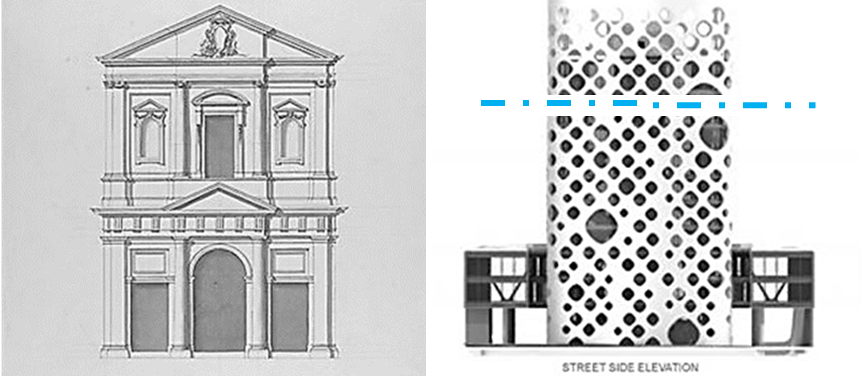
\includegraphics[width= \linewidth]{Images/BaroqueVsContemporaryfacade}
%          \caption{Evolution of facade design.
%          Baroque Facade 1639 by Bernini (left) vs Contemporary facade, building O-14 by Reiser + Umemoto, 21st Century (right) (\textit{Images edited from source)}}
%          \label{fig:FacadeBaroqueVsContemporary}
%        \end{figure}
%
%However, much like the broader scope of architecture, the role of ornamentation and facades has also undergone evolution and transformation throughout history.
%To elucidate how various societies and civilizations have conveyed their identity through architectural ornamentation and symbolism, we embark on an exploration of the interpretations given to facades by some of the most influential architects and artists of their respective eras.
%
%%!%Facade according to Vitruvius
%
%Vitruvius, a celebrated Roman architect and military engineer, in 1st century BCE, author of ``De Architectura'', a series of ten books considered as the first treatise in architecture theory\cite{Kruft1994}.
%Within this work, Vitruvius advocates for three essential attributes that a building should embody: ``firmitas'' (structural soundness), ``utilitas'' (functionality), and ``venustas'' (beauty or aesthetics)\cite{Ostwald2023}.
%
%Vitruvius places emphasis primarily on Reason, and secondarily on proportions.
%It's worth highlighting that the cultural atmosphere in ancient Rome during the late first century B.C favoured the understanding of the world as a well-structured and ordered whole\cite{Lefas2000}.
%
%Facades partake of this reasoning and in accordance to Vitruvius should not only be visually appealing but should also reflect the underlying structural integrity of the building and fulfill its intended purpose effectively(Figure\ref{fig:Vitruvianarchitecture}).
%In terms of ornamentation, Vitruvius seeks to approach this subjective realm, dominated by taste, with objectivity.
%He rationalizes that a pleasing appearance emerges from the harmony and balance among the components that constitute a composition\cite{Lefas2000}.
%
%%% Figure of vitruvian Architecture
%    \begin{figure}[htb]
%        \centering
%        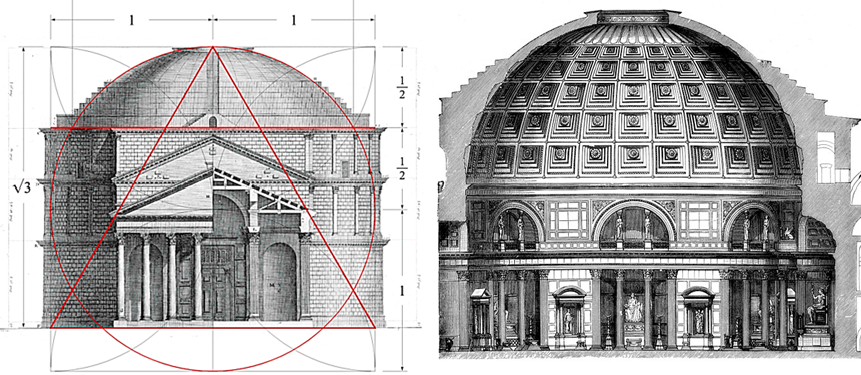
\includegraphics[width= \linewidth]{Images/VitruvianArchitecture}
%        \caption{Facade and ornament according to Vitruvius, with emphasis in order symmetry and harmony. Pantheon's facade (left) and cross section(right) symmetry analysis (\textit{Images edited from source)}}
%        \label{fig:Vitruvianarchitecture}
%    \end{figure}
%
%Additionally, Vitruvius determines that the deciding factor for those components would follow the principle of ``Decor'',  the  fifth  principle on his system of values that elevates simple  building  practice  into  architecture, defined as the property that  deals  with  the  «appropriate»  articulation and construction of the work on principles respecting religion, nature and social conventions\cite{Lefas2000}.
%
%In essence, according to Vitruvius, facades and their ornamentation stem from a sense of order and rationality.
%They are achieved through a harmonious equilibrium of well-considered elements that adhere to established principles, while taking into account both tradition and nature.
%This approach aims to achieve beauty while also effectively fulfilling the intended purpose of the facade.
%
%Vitruvius's contributions would have a lasting impact on the field of construction spanning centuries.
%However, his work remained largely dormant for a considerable period until its revival during the Renaissance, which encompassed the 14th to the 17th century.
%
%This resurgence continued during the Neoclassical style of the 18th century and the Ecole des Beaux-Arts style of the 19th and early 20th centuries.
%This series of revivals and reinterpretations led to the rekindling of Classical architecture in the years that followed\cite{Wikipedia2023}(Figure\ref{fig:ClassicismNeoClassicism}).
%
%%% Figure of Classicism and Neo classicism facade
%     \begin{figure}[htb]
%          \centering
%          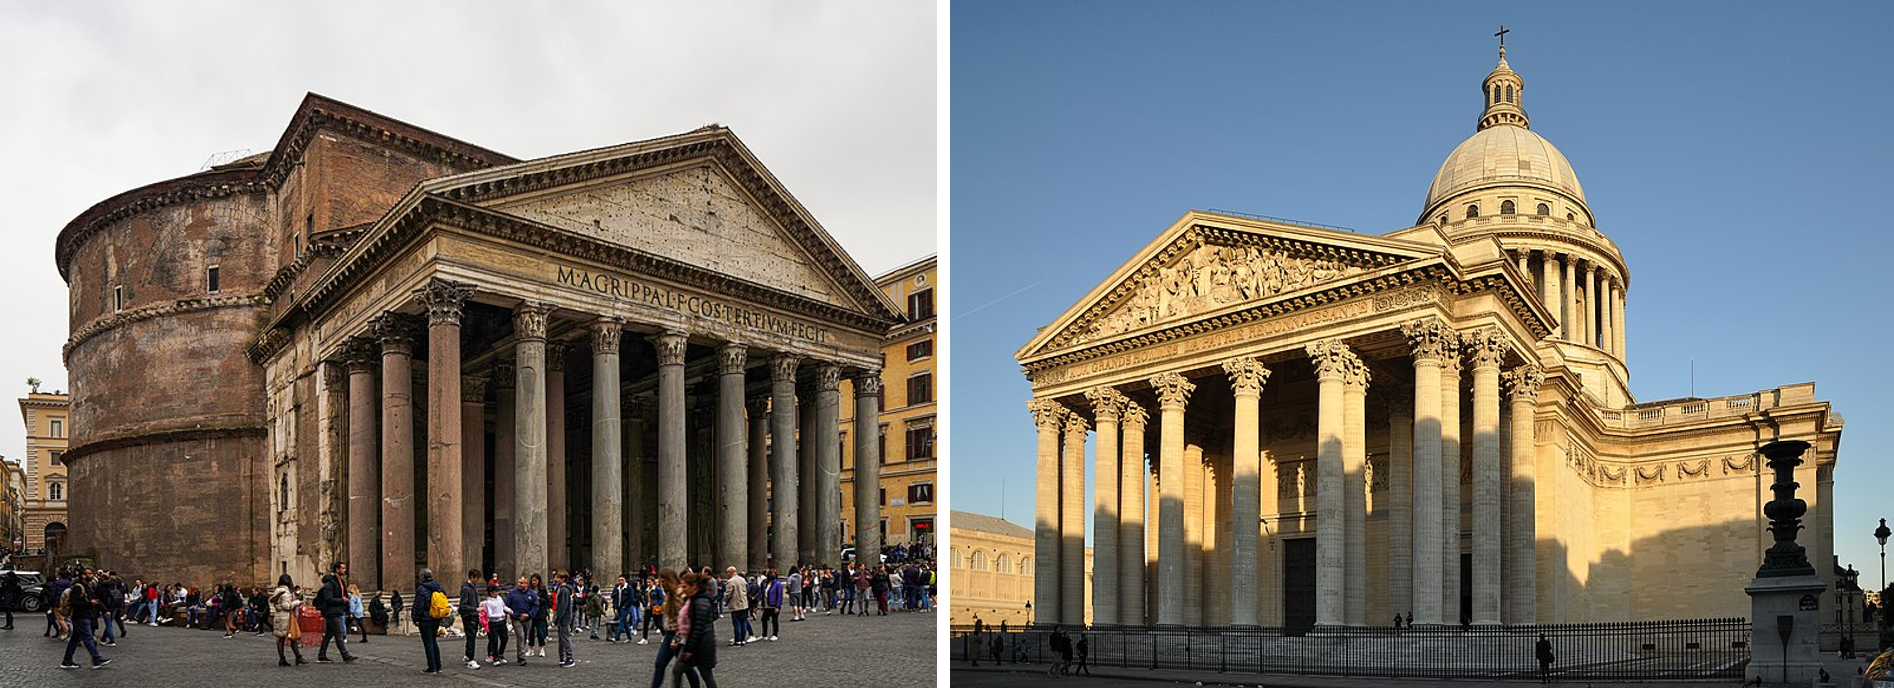
\includegraphics[width= \linewidth]{Images/ClassicismNeoClassicism}
%          \caption{Continuity of Vitruvius' Influence: Classicism and Neoclassicism in Facades and Ornamentation. Architectural aesthetics rooted in order and rationality. (Left) Pantheon in Rome, constructed in 27 BC. (Right) Pantheon in Paris, erected between 1758 and 1790, Neoclassical Approach in the Mid-18th Century. (\textit{Images edited from source)}}
%          \label{fig:ClassicismNeoClassicism}
%        \end{figure}
%
%%!%facade according to bernini and borromini
%Moving beyond the Renaissance era and into the Baroque style, a significant shift in the perception of facades and ornamentation occurs.
%Francesco Borromini, a prominent Italian architect of the Baroque period, emerges as a key figure in this context.
%
%In his exploration of facades, Borromini emphasized the dynamic relationship between a building's interior and its facade, as a form of movement of matter beyond the body, precisely because the generation of form is internal to the object itself\cite{Benjamin2006}, therefore the facade should serve as a visual representation of the internal spaces and functions of the building.
%
%Borromini's approach to facades went beyond mere decorative elements.
%He saw the facade as an opportunity to express the inner workings and spatial organization of the building.
%This concept is reflected in his designs, where facades often featured intricate geometric patterns, curved forms, and sculptural elements that hinted at the internal arrangements of rooms and structures(Figure\ref{fig:BorrominiArchitecture}).
%
%%% Figure of Baroque facade Borromini
%     \begin{figure}[htb]
%          \centering
%          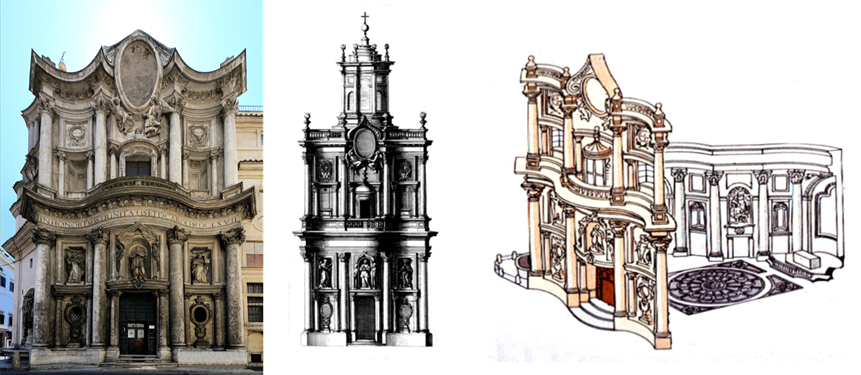
\includegraphics[width= \linewidth]{Images/BaroquefacadeBorromini}
%          \caption{Borromini's Interpretation of Facade and Ornament: Elaborate geometric patterns, curved forms, and sculptural elements reflecting internal spatial arrangements. Analysis of San Carlo alle Quattro Fontane Church Facade (left) and Cross Section (right) from its construction in the 1630s, Rome. (\textit{Images edited from source)}}
%          \label{fig:BorrominiArchitecture}
%        \end{figure}
%
%``Exteriors which expressively display interiorities;
%interiors which fold from within and, [\ldots] which appear to invite an exterior reading while presenting an interiorized text''\cite{Biglieri2004}.
%In essence, Borromini's perspective on facades went beyond surface aesthetics;
%he considered them as integral components of the architectural composition that could convey deeper meanings about the building's design and purpose.
%
%%! context on neo classic, art nouveau and art deco
%
%Exploring the historical evolution of facades and ornamentation necessitates acknowledging distinct periods that have significantly contributed to the advancement of architectural practice.
%
%In the trajectory from Baroque to the transformative epoch of Modernism, various architectural styles emerged, yet none attained the global influence and profound impact comparable to the preceding Classicism, which drew inspiration from the ideals of Vitruvius, and subsequently Modernism on the 20th century would bring.
%
%For the purpose of this research, before delving into the profound shifts of Modernism, it's crucial to acknowledge certain periods that contributed to architectural understanding without causing radical shifts.
%
%Chronologically, the evolution from Baroque to Modernism included styles like Rococo, Neoclassical, Romanticism, Gothic Revival, Victorian, Arts and Crafts, Art Nouveau, and Art Deco, each leaving their mark on architectural expression.
%
%Notably, Neo-Classicism, Art Nouveau, and Art Deco stand out as particularly influential periods.
%
%The Neo-Classical style of the late 18th to early 19th centuries, with a resurgence through the École des Beaux-Arts in Paris during the late 19th to early 20th centuries, reflected facades and ornamentation rooted in Vitruvian Principles and Palladian Architecture.
%It emphasized formal elegance, symmetry, and grandeur, often featuring facades with balanced proportions flanked by columns (Figure\ref{fig:ClassicismNeoClassicism}).
%
%The Art Nouveau style of the late 19th to early 20th centuries, prominent in Europe, introduced ornamentation and facades with an organic character.
%This style, exemplified by figures like Gaudi, drew inspiration from nature's forms and flow lines.
%Gaudi's work, for instance, used flowing,  wavy,  and  naturally  curvilinear lines that mirrored natural shapes, and mosaic-like tiles mimicking textures and colors of the natural world\cite{Nasir2022} (Figure\ref{fig:ArtNouveaustyle}).
%
%%% Figure of Art Nouveau style  facade
%     \begin{figure}[htb]
%          \centering
%          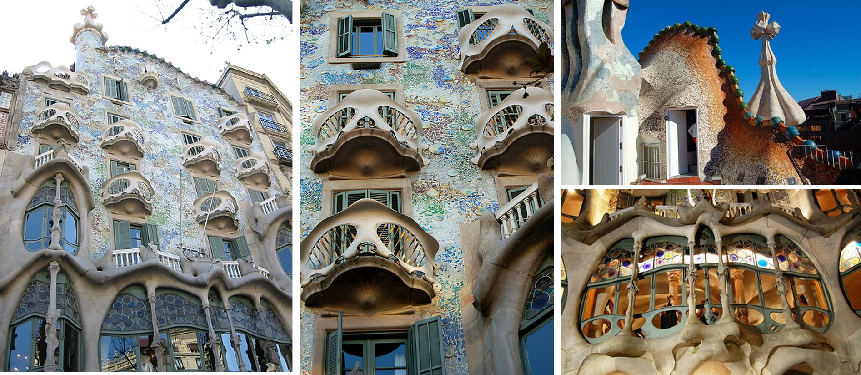
\includegraphics[width= \linewidth]{Images/ArtnouveauGaudi}
%          \caption{Facade and ornament according to Art Nouveau style inspired in organic forms, illustrated by Casa Batlló in Barcelona, 1904, designed by Antoni Gaudi. (Left) Casa Batlló's iconic facade. (Middle) A close-up of the intricate mosaic work and balconies. (Upper Right) Ornate mosaic patterns on the roof and (Down Right) windows echoing the textures and colors of the natural world. (\textit{Images edited from source)}}
%          \label{fig:ArtNouveaustyle}
%        \end{figure}
%
%While the Art Deco style prevalent in Europe and America during in the 1920s to early 1930s will come to rethink Facade and Ornament through the prisms of luxury and technological progress.
%
%Characterized by its distinct attributes, Art Deco places an emphasis on crisp lines, striking geometric shapes often arranged symmetrically, and a vivid palette of high-contrast, intense colors.
%This visual impact is further heightened by the incorporation of metallic surfaces, contributing to an overall ornamental effect that catches the eye\cite{Kotb2014}.
%
%This style aimed to capture both modernity and historical nostalgia, resulting in a fusion of futuristic aspirations and references paying homage to the past (Figure\ref{fig:ArtDeco}).
%
%%% Figure of Art Deco style  facade
%     \begin{figure}[htb]
%          \centering
%          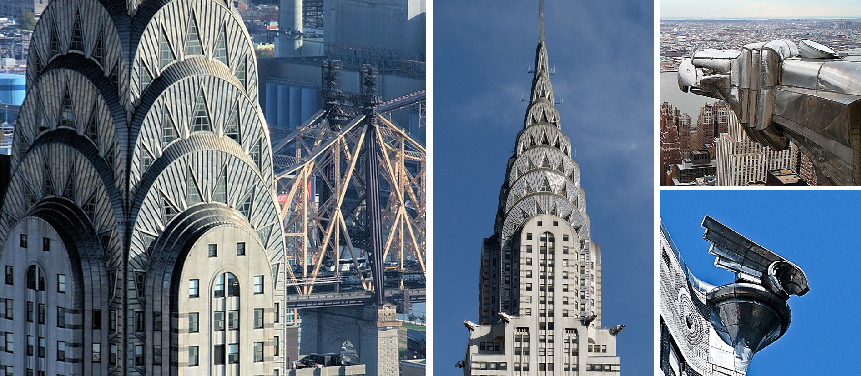
\includegraphics[width= \linewidth]{Images/ArtDecoFacade}
%          \caption{Art Deco Aesthetic of the 1920s to Early 1930s:Art Deco Approach in the 1920s to Early 1930s:  Illustrated by the Chrysler Building, completed in 1930. Facade (Left) and ornamental details (Right) harmonizing futuristic aspirations with references paying homage to the past. (\textit{Images edited from source)}}
%          \label{fig:ArtDeco}
%        \end{figure}
%
%However, while these styles undoubtedly added depth and variety to architectural aesthetics, they did not bring about the same profound paradigm shifts that would later characterize the Modernist movement.
%
%With this broader context established, the analysis will now shift its focus to the Modernist movement's transformative impact on architectural philosophy.
%
%%! Modernism and facade according to Le Corbusier
%
%Transitioning from the Baroque style, where facades became expressions of internal dynamics, and acknowledging the enriched insights from the Neoclassical, Art Nouveau and ArtDeco Style,  the historical evolution of facades and ornamentation takes us into the Modernist style of the 20th century—a pivotal juncture that marked one of the most significant shifts in architectural theory.
%
% Within this era, a radicalized interpretation of ``Form follows function'' emerged, embodying a profound departure from the conventional understanding of facades and ornamentation, partly due to a prevailing stance against ornamentation, often dismissed on moralistic grounds.
%
%Adolf Loos' 1908 article ``Ornament and Crime'' exemplified this sentiment by advocating functional design and condemning conventional ornamentation as unnecessary\cite{Saglam2014}.
%
%Le Corbusier, one of the most prominent figures of this epoch, and renowned for his influential work ``Towards a New Architecture'' first published in 1923, and considered by some to be the most important architectural work published in the 20th century, epitomized the spirit of the era with his distinct views on facades and ornamentation\cite{Studio2a2023}.
%
%Embracing a minimalist and utilitarian approach, Le Corbusier believed that a facade should mirror a building's internal functions, designed in alignment with its purpose and occupants' needs.
%
%Rooted in a human-centric design philosophy, his mantras ``Constructing the architecture of men'' and ``Men are the ones who truly matter'' underscored his commitment to prioritizing people's well-being in his designs\cite{Virseda2021}.
%
%His manifesto ``The Five Points of a New Architecture'' further solidified his design principles.
%The notion of ``Free design of the facade'' attained by separating the exterior of the building from its structural function is presented as the means through which the facade liberates itself from conventional structural limitations\cite{Corbusier1986}.
%
%This allowed for the incorporation of large expanses of windows to provide ample natural light and ventilation, fostering a seamless connection between the interior and exterior realms.
%
%Even during this era when ornamentation was viewed unfavorably, Le Corbusier believes in a form of functional ornamentation, as Venturi\cite{Venturi1972} would later accurately point out, Modern architecture uses expressive ornament and shuns explicit symbolic  ornament.
%
%He would ingeniously devise methods to infuse his creations with a distinct form of ornamentation, albeit one rooted in materials' textures, structural elements, and inventive ways of articulating functionality\cite{Saglam2014} that emerged from the building's design.
%
%For example, he used sunshades, brise-soleil, and other shading devices as a way to address climate and control light without compromising the building's aesthetic integrity.
%
%In essence, Le Corbusier's viewpoint on facades and ornamentation epitomized clarity, rationality, and harmonious integration.
%His architecture rejected superfluous adornment, and celebrated both technological advancements and structural innovation while maintaining a genuine focus on the well-being and experiences of the occupants (Figure\ref{fig:Modernistfacade}).
%
%%% Figure of Modernist facade and ornament by Le corbusier
%     \begin{figure}[htb]
%          \centering
%          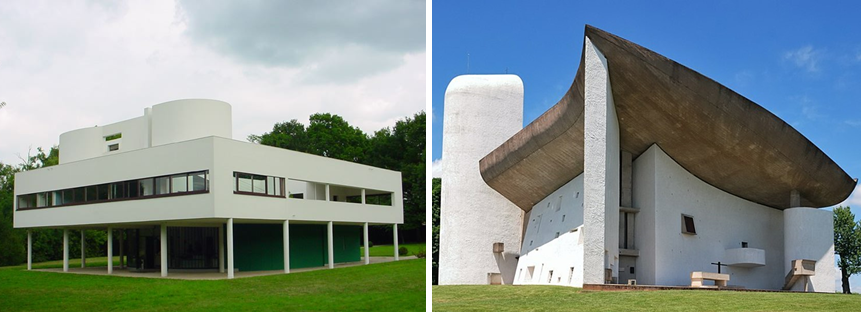
\includegraphics[width= \linewidth]{Images/ModernistFacade}
%          \caption{Evolution of Functionalism: Le Corbusier's Journey towards Modernist Facade and Ornamentation. (Left) Villa Savoye, 1928--1931. (Right) Chapelle Notre-Dame-du-Haut de Ronchamp, 1955 (\textit{Images edited from source)}}
%          \label{fig:Modernistfacade}
%        \end{figure}
%
%%! Postmodernism and facade according to Venturi
%
%However, despite the innovative ideals of the Modernist movement,  it became apparent that its utopian vision didn't always materialize as intended.
%While the pursuit of functionalism and simplicity was meant to create efficient and logical designs, the outcomes were not always aligned with the intended human experiences.
%
%The Modernist approach often led to the unintentional creation of spaces that felt monotonous and detached from their cultural contexts.
%The emphasis on minimalism and the rejection of ornamentation sometimes resulted in environments lacking a sense of identity and character.
%
%The architectural pursuit of universality and timelessness would instead produce sterile, glass-cube structures\cite{Schudel2018} disregarding the importance of cultural heritage and local context, and inadvertently raise the question: Is the reinvention of form, that rejected explicit symbolism and frivolous applique ornament, inspired by the modernist ideals, yielding a Heroic and original outcome, or is it, instead, a dry expressionism, empty and boring that has distorted the whole building into one big ornament\cite{Venturi1971}.
%
%This scrutiny of the Modernist movement's inability to adequately encompass human experiences and cultural significance, which sparked controversy during the 1960s, brings us to the influential ideas of architect and theorist Robert Venturi.
%
%Venturi's book ``Complexity and Contradiction in Architecture'', published in 1966, marked a turning point in architectural discourse and challenged the prevailing modernist ideals.
%
%Robert Venturi, an iconoclastic architect often hailed as the pioneer of postmodernism\cite{Schudel2018} stood firmly against the oversimplification of architecture, championing the incorporation of contradiction and complexity to yield authentic and vital creations.
%
%The modernist ideals, heavily favoring automobile-centric urban planning, influenced the formation of cities that catered to cars rather than people.
%
%In their thought-provoking book from 1972, ``Learning From Las Vegas'', Venturi et al.\cite{Venturi1972} put forth a compelling argument, exemplified by the stark contrast seen in places like Las Vegas, they assert that if you were to strip away the dazzling signs, what remains is not a thriving urban environment but a barren desert.
%
%This analogy underscores the extent to which architecture had been relegated to a mere functional necessity camouflaged behind attention-grabbing signs.
%
%Venturi et al.\cite{Venturi1972} will further explain that the oversimplification of architecture, combined with the emergence of sprawling spaces, high speeds, and intricate functions where symbols hold more significance than actual forms, has transformed architecture into symbols occupying space, rather than forming it.
%
%This shift implies that the architectural structure itself carries minimal meaning, with the focus primarily directed towards the signs that communicate with it.
%
%The building stands isolated from the street, often separated by vast parking lots, while the front-facing sign juts out perpendicular to the highway, detached from the building.
%At the rear, the structure becomes a utilitarian afterthought, reduced to a budgetary obligation\cite{Venturi1972}.
%
%In this scenario, the absence of signs leaves behind a vacuous atmosphere, characterized by scattered buildings that lack enclosure and cohesion.
%The architecture loses its essence, mirroring a cultural void much like a desert devoid of life and enrichment.
%
%The impact of these dynamics is not confined to the past;
%instead, they continue to reverberate through the present state of our cities.
%Many urban landscapes today still adhere to the principles that emerged from the modernist era.
%The prioritization of cars and the resulting sprawling infrastructure persist in shaping cityscapes that often prioritize functionality over human experience.
%
%In response to the challenges posed by the Modernist movement and its unintended consequences, Venturi would reshape the course of architectural discourse.
%Notably, he will famously invert the famous dictum of Mies van der Rohe ‘Less is more’ into ‘Less is a bore'\cite{Lutolli2020}, encapsulating his bold departure from the prevailing architectural norms.
%
%In his book ``Complexity and Contradiction in Architecture''\cite{Venturi1977}, Venturi emphasized that architecture should be responsive to the cultural context and the people who inhabit it.
%
%His viewpoint marked a departure from the rigid modernist principles who shunned symbolism of form as an expression or reinforcement of content that dictated that architectural form was to be determined solely by program and structure, with an  occasional  assist from  intuition\cite{Venturi1972}.
%
%Instead, he proposed a reevaluation of the role of ornament and complexity in architectural design (Figure\ref{fig:Middletimeline} d).
%
%%% Figure of Postmodernism facade and ornament
%     \begin{figure}[htb]
%          \centering
%          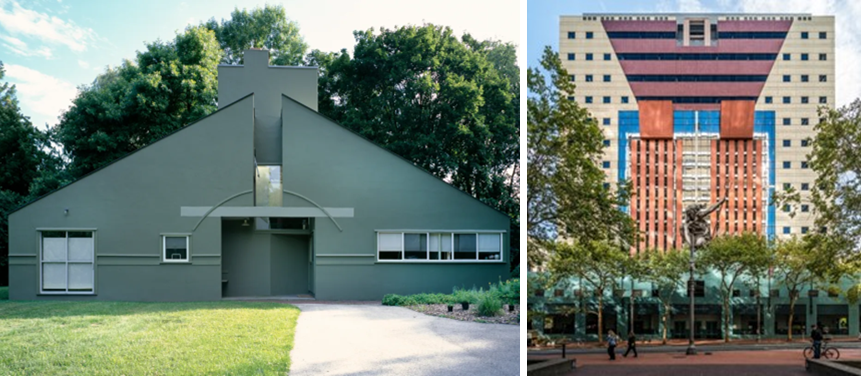
\includegraphics[width= \linewidth]{Images/PostmodernismVenturi}
%          \caption{Postmodernism and the advent of complexity and contradiction (Left) Vanna Venturi House, designed by Robert Venturi and Denise Scott Brown in 1964. (Right) Portland Municipal Services Building, designed by Michael Graves, in 1982 (\textit{Images edited from source)}}
%          \label{fig:postmodernfacade}
%        \end{figure}
%
%On this context, Venturi believed that a facade could communicate various meanings, evoke emotions, and respond to its cultural and contextual surroundings.
%
%Venturi emphasized the richness of symbolism within architecture, asserting that symbols were fundamental in the architectural language, advocating for the integration of elements from historical precedents and the existing urban fabric, treating them as source materials that could be intelligently referenced or replicated to inform the design process\cite{Venturi1971}.
%
%Importantly, Venturi's approach did not solely prioritize outward appearance;
%it was deeply intertwined with the functional aspects of a building's interior, aligning with his belief that architecture should serve both utilitarian purposes and evoke meaningful experiences.
%
%Regarding ornament, he argued that ornamentation was not inherently negative but should be used judiciously and meaningfully.
%
%Venturi coined phrase ``Less is a bore'', suggests his approach towards ornament in what he would describe as ``the decorated shed''\cite{Venturi1972} that architecture doesn't have to be stripped of ornamentation to be considered valid.
%
%His approach to facades, and for those that shared the postmodern movement,involved a deliberate use of various elements to add depth and complexity.
%These included decorative elements like ornate moldings, intricate carvings, references to classical motifs, fragmentation of forms and the use of bright colors and patterns in the arrangement of the facade\cite{McLaughlin2023}.
%
%Rather than adhering to a single architectural style, Venturi purposefully juxtaposed different styles, often expressed through a variety of materials and textures.
%This approach aimed to create a visually stimulating experience by embracing the concept of contradiction (Figure\ref{fig:postmodernOrnamnet}).
%
%%% Figure of Postmodernism ornament
%     \begin{figure}[htb]
%          \centering
%          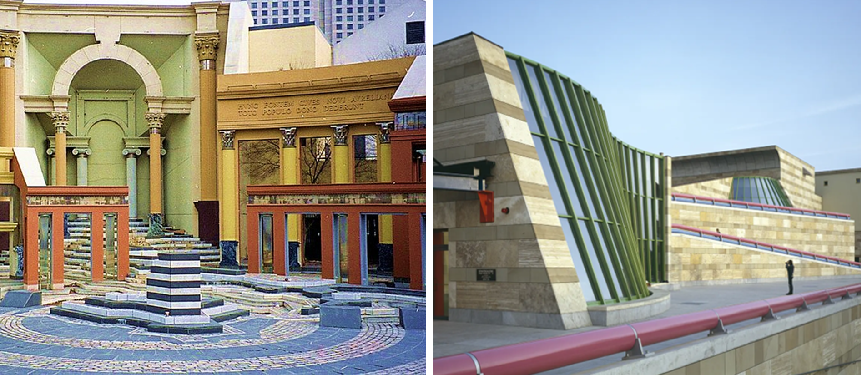
\includegraphics[width= \linewidth]{Images/PostmodernOrnament}
%          \caption{Postmodernism approach to ornament using referencing different historical styles in a variety of materials and colors to create complexity. (Left) The Piazza d’Italia, New Orleans, designed by  postmodernist Charles Moore and Perez Architects, built in 1978. (Right) Neue Staatsgalerie, Stuttgart, Germany, designed by James Stirling, built in 1984 \textit{(Images edited from source)}}
%          \label{fig:postmodernOrnamnet}
%        \end{figure}
%
%Furthermore, Venturi's designs exhibited a sense of playfulness.
%He introduced references to historical styles, cultural symbols, and contextual connections, adding layers of meaning to his designs.
%
%This approach to ornamentation went beyond mere decoration;
%it sought to enrich the architectural experience by engaging with diverse influences and creating a dialogue with the surrounding environment.
%
%In essence, Robert Venturi's perspective on facades and ornamentation underscored the significance of welcoming diversity, historical resonance, and meaningful expression within architectural design.
%
%His vision urged contemporary architects to recognize a crucial reality—perfection within the architectural realm is not confined to flawless forms but also encompasses the beauty found in imperfection, across its myriad manifestations\cite{Lutolli2020}.
%
%This eclectic and innovative approach, which drew inspiration from a renewed appreciation for historical ornamentation, boldly expanded the horizons of architectural exploration throughout the 20th century\cite{Stamp2016} paving the way for the bold explorations and boundary-pushing experiments that would characterize the late 20th century.
%
%%! Contemporary styles start
%
%As the 20th century progressed, architecture continued to evolve, building upon the foundations laid by modernism and postmodernism.
%This era witnessed a shifting design sensibility, marked by a more dynamic and diverse approach, particularly evident in the treatment of facades and ornamentation.
%
%We have previously stated the argument that the history of architecture, and the essence of architecture evolution, consists of an ever-changing interplay between simplicity and complexity.
%
%In the aftermath of Postmodernism, the realm of architecture saw a diverse array of styles emerge, each carrying forward unique interpretations of facades and ornamentation in an apparent trend towards more complex design.
%
%As Hopkins\cite{Hopkins2020} elaborates, while modernism sought clarity and simplicity in its facades, and aimed to distill architecture to its essential fundamentals, postmodernism adopted a contrasting approach embracing complexity and ornamentation and just adding more ideas, symbols on an effort to communicate what it does.
%
%This shift marked a transition from abstract and minimalist aesthetics to a more descriptive and communicative style.
%
%Contemporary architecture emerged as a synthesis of these previous movements.
%In the realm of ornamentation, contemporary architects found a middle ground, recognizing the potential of ornament to convey meaning, context, and identity.
%
%Ornamentation in contemporary architecture often took on a more purposeful role, serving as a bridge between tradition and innovation.
%
%The ornamentation became a language through which buildings could communicate their cultural relevance, while also responding to the demands of a rapidly changing world.
%
%Influenced by the advent of computer-aided design and advancements in technology, as well as driven by a sustainability agenda emphasizing efficient resource utilization, the architectural world of the late 20th century and the current 21st century has witnessed the emergence of several prominent architectural styles.
%
%While this era lacks a unified movement, the different styles have collectively left an indelible mark on the field of architecture.
%
%These styles include Deconstructivism, Neofuturism, High-tech modernism, Parametricism, and Pragmatic utopianism, each offering a unique perspective on architecture and design (Figure\ref{fig:contemporarytimeline}).
%
%%% Figure of Contemporary timeline
%     \begin{figure*}[htb]
%          \centering
%          \includegraphics[width= \linewidth]{Images/contemporaryTimeline}
%          \caption{Contemporary architecture. An era of exploration. (from left to right) Desconstructivism, Neofuturism, High-tech modernism, Parametricism, Pragmatic utopinaism.  (\textit{Images edited from source)}}
%          \label{fig:contemporarytimeline}
%        \end{figure*}
%
%%! Deconstructivism
%
%In the realm of Deconstructivism, which gained prominence in the 1980s\cite{Clement2017}, architects like Frank Gehry pioneered a distinct interpretation of ornamentation taking on an unconventional and dynamic character (see Figure\ref{fig:contemporarytimeline} \textit{a}).
%
%Deconstructivism facades challenge traditional notions, introducing the concepts of fragmentation, and fracture with non-rectilinear shapes which serve to distort and dislocate conventional building elements in a deliberate and provocative manner.
%
%Ornamentation in this context is not applied in the traditional sense but is rather an intrinsic part of the building, such as structure and envelope and an interest in handling ideas of a structure’s surface or skin\cite{Clement2017}.
%The Guggenheim museum in Bilbao, built in 1997, is a primary example of this approach towards architecture.
%
%%! Neofuturism
%
%Transitioning from the realm of Deconstructivism, let's now explore Neofuturism, a design movement that gained prominence in the late 20th and early 21st centuries and continues to exert influence in contemporary architecture.
%This style finds a compelling embodiment in the work of Santiago Calatrava\cite{Omale2016}.
%
%His architectural creations, exemplified by iconic structures like the Milwaukee Art Museum (refer to Figure\ref{fig:contemporarytimeline} \textit{b}), constructed in 2001, defy conventional perceptions of facades with their dynamic, seemingly in-motion forms\cite{Tyc2018}.
%
%Neofuturism's approach to facades and ornamentation is deeply rooted in a futuristic and avant-garde aesthetic, celebrating the transformative potential of technology and the beauty of technical achievements as an art form\cite{Tyc2018}.
%
%In contrast to the radical functionalism of modernism, Neofuturism embraces a more comprehensive functionalism.
%It recognizes a multitude of functionality aspects within architectural design, including structural, pragmatic, symbolic, and social functions, as integral components of the creative process.
%Moreover, Neofuturism extends its considerations to encompass environmental, urban, ethical, and aesthetic factors, all of which contribute significantly to shaping the architectural expression\cite{Omale2016}.
%
%Characterized by sleek lines, innovative materials, and an unwavering focus on technology and functionality, Neofuturist facades lean towards minimalism.
%These facades often employ steel, glass, and concrete materials, emphasizing geometric forms as key design elements\ref{fig:neofuturism}.
%
%%% Figure of neofuturism
%     \begin{figure}[htb]
%          \centering
%          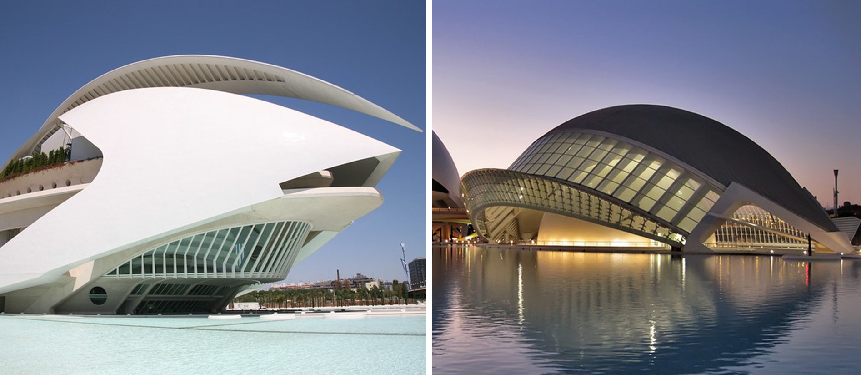
\includegraphics[width= \linewidth]{Images/neofuturism}
%          \caption{Neofuturism approach to facades and ornament. (Left) Queen Sofia Palace of Arts, Valencia, Spain, designed by Santiago Calatrava , built in 2005. (Right) The City of Arts and Sciences, designed by Santiago Calatrava, built in 1996. \textit{(Images edited from source)}}
%          \label{fig:neofuturism}
%        \end{figure}
%
%Neofuturist ornamentation tends to be seamlessly integrated into the building's structure and materials, prioritizing simplicity and clean lines.
%The movement seeks to convey a powerful sense of progress, innovation, and a visionary perspective of the future through its architectural designs.
%
%%! High tech modernism
%
%Building upon the theme of technological integration, another prominent architectural style that emerged during the late 20th century, known as high-tech modernism or structural expressionism extends the exploration of facades and ornamentation in a distinctly different direction.
%
%While neofuturism expresses its futuristic vision through dynamic forms and sleek materials, often resulting in monumental structures reminiscent of a futuristic science fiction movie, high-tech modernism takes a more measured approach.
%
%This architectural style explores the aesthetic and functional potentials of advanced technology with a sense of refinement and restraint(refer to Figure\ref{fig:contemporarytimeline} \textit{c}).
%
%High-tech modernism is characterized by its emphasis on technological innovation, transparency, and structural expression.
%Renzo Piano and Norman Foster are influential architects associated with the high-tech modernist movement\cite{Tyc2018}.
%
%Iconic works like The Shard (designed by Renzo Piano) and the Gherkin building (designed by Foster + Partners), both located in London, exemplify the essence of high-tech style (Figure\ref{fig:hightechmodernism}).
%
%%% Figure of hightech modernism
%     \begin{figure}[htb]
%          \centering
%          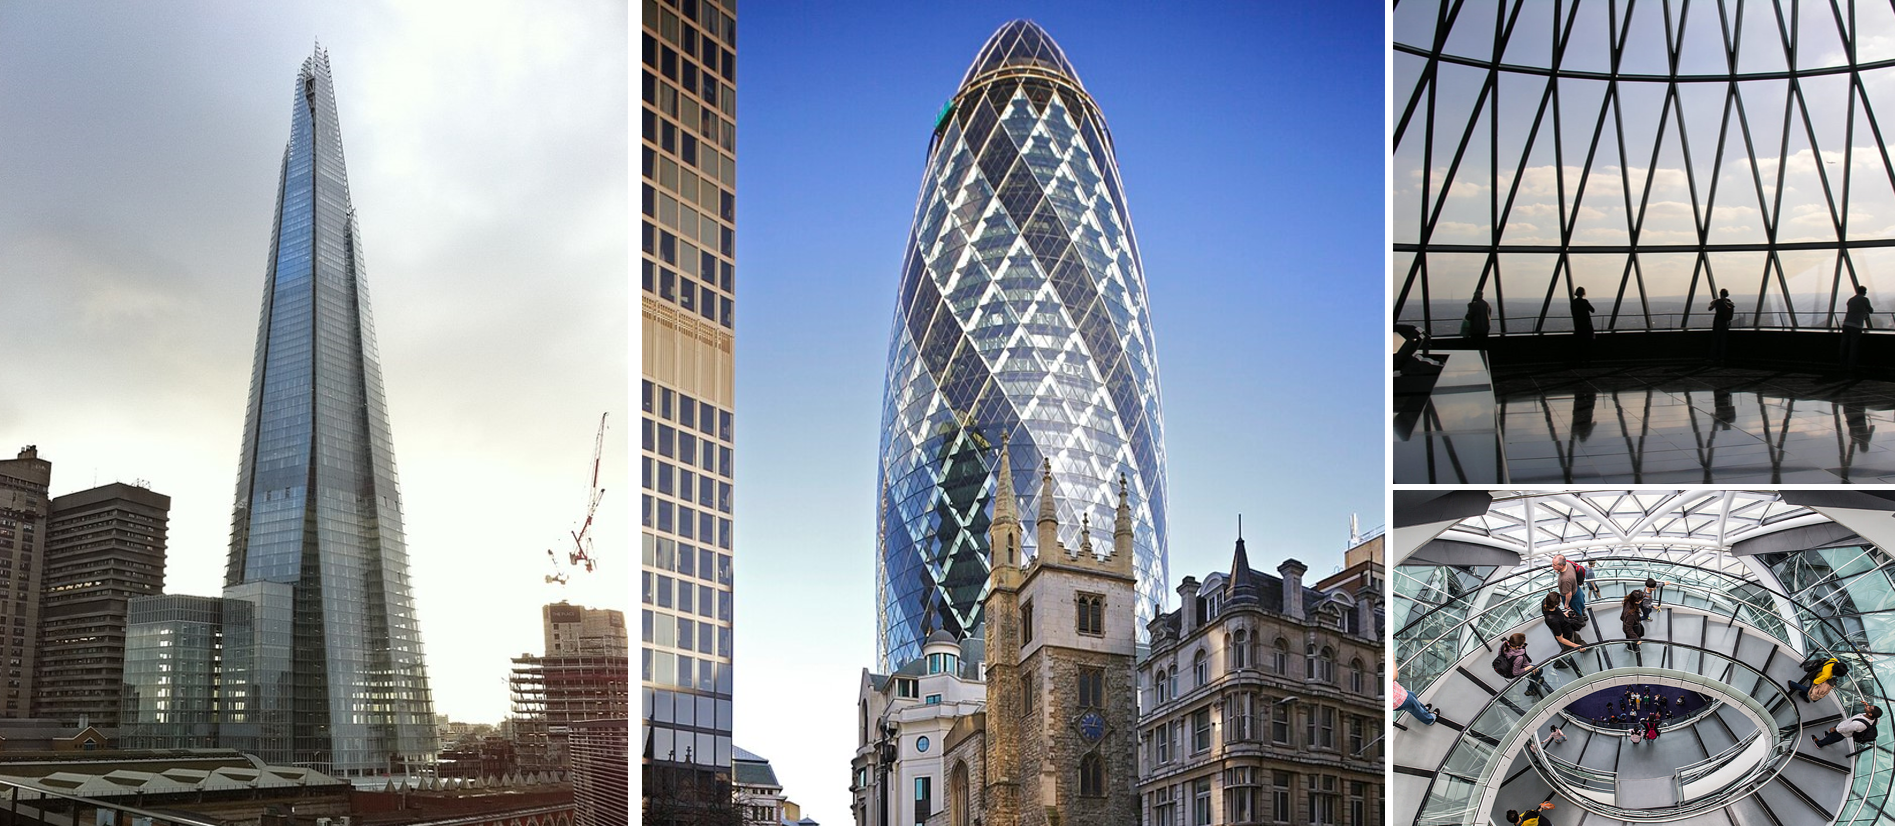
\includegraphics[width= \linewidth]{Images/hightechmodernism}
%          \caption{High-tech Modernism approach to facades and ornament. (Left) The Shard, London, England, designed by Renzo Piano, built in 2012. (Right) Exterior and interior views of The Gherkin building, London, England, designed by  Foster + Partners, built in 2003 \textit{(Images edited from source)}}
%          \label{fig:hightechmodernism}
%        \end{figure}
%
%In terms of facades and ornamentation, high-tech modernism often features exposed structural elements, innovative use of materials like glass and steel, and a focus on showcasing the building's inner workings.
%
%This approach aligns seamlessly with the ethos of high-tech architects, who hold technological advancement in high regard as a driving force for architectural innovation and expression, as emphasized by Davies\cite{Davies1988}.
%
%The aim is to showcase the building's technological components and express its functionality while maintaining a sleek and minimalist appearance.
%High-tech modernism prioritizes functionality and efficiency while celebrating the aesthetic possibilities of modern technology and machines.
%
%Le Corbusier coined the phrase ``house as a machine for living in,'' yet his own architectural creations, while inspired by this idea, remained technologically rudimentary and lacked the appearance of machines.
%
%In contrast, High Tech buildings distinctly embody the machine aesthetic, they do look like machines.
%This is not just a metaphor but a tangible source of both technology and visual inspiration\cite{Davies1988}.
%
%It's a departure from traditional ornamentation, favoring a more industrial and minimalist aesthetic that emphasizes the beauty of engineering and technology itself.
%
%%! Parametricism
%
%In contrast to the emphasis on technological innovation and transparency seen in high-tech modernism, parametricism, another architectural style emerging in the late 20th century and evolving into the 21st century, takes a distinctive approach.
%Often associated with renowned architects like Zaha Hadid, parametricism represents a response to technological advances, particularly in computational design (Figure\ref{fig:contemporarytimeline} \textit{d}).
%
%Parametricism explores the integration of computational design and intricate geometries to create structures that challenge conventional ideas of facades and ornamentation.
%Central to this style is the concept that all architectural elements and complexes can be shaped and adjusted through parametric means, a principle articulated by Schumacher\cite{Schumacher2010}.
%
%Within the realm of parametricism, facades undergo a remarkable transformation, becoming dynamic and adaptive to environmental and contextual factors.
%The rigid lines of traditional architecture give way to sinuous curves and intricate patterns, characterizing its formal repertoire that departs from monotonous repetition and rigid functional stereotypes\cite{Schumacher2008}.
%
%Zaha Hadid's iconic designs, such as the Heydar Aliyev Center in Baku and the Guangzhou Opera House, exemplify this transformative approach to architecture (Figure\ref{fig:Parametricism}).
%
%%% Figure of parametricism
%     \begin{figure}[t]
%          \centering
%          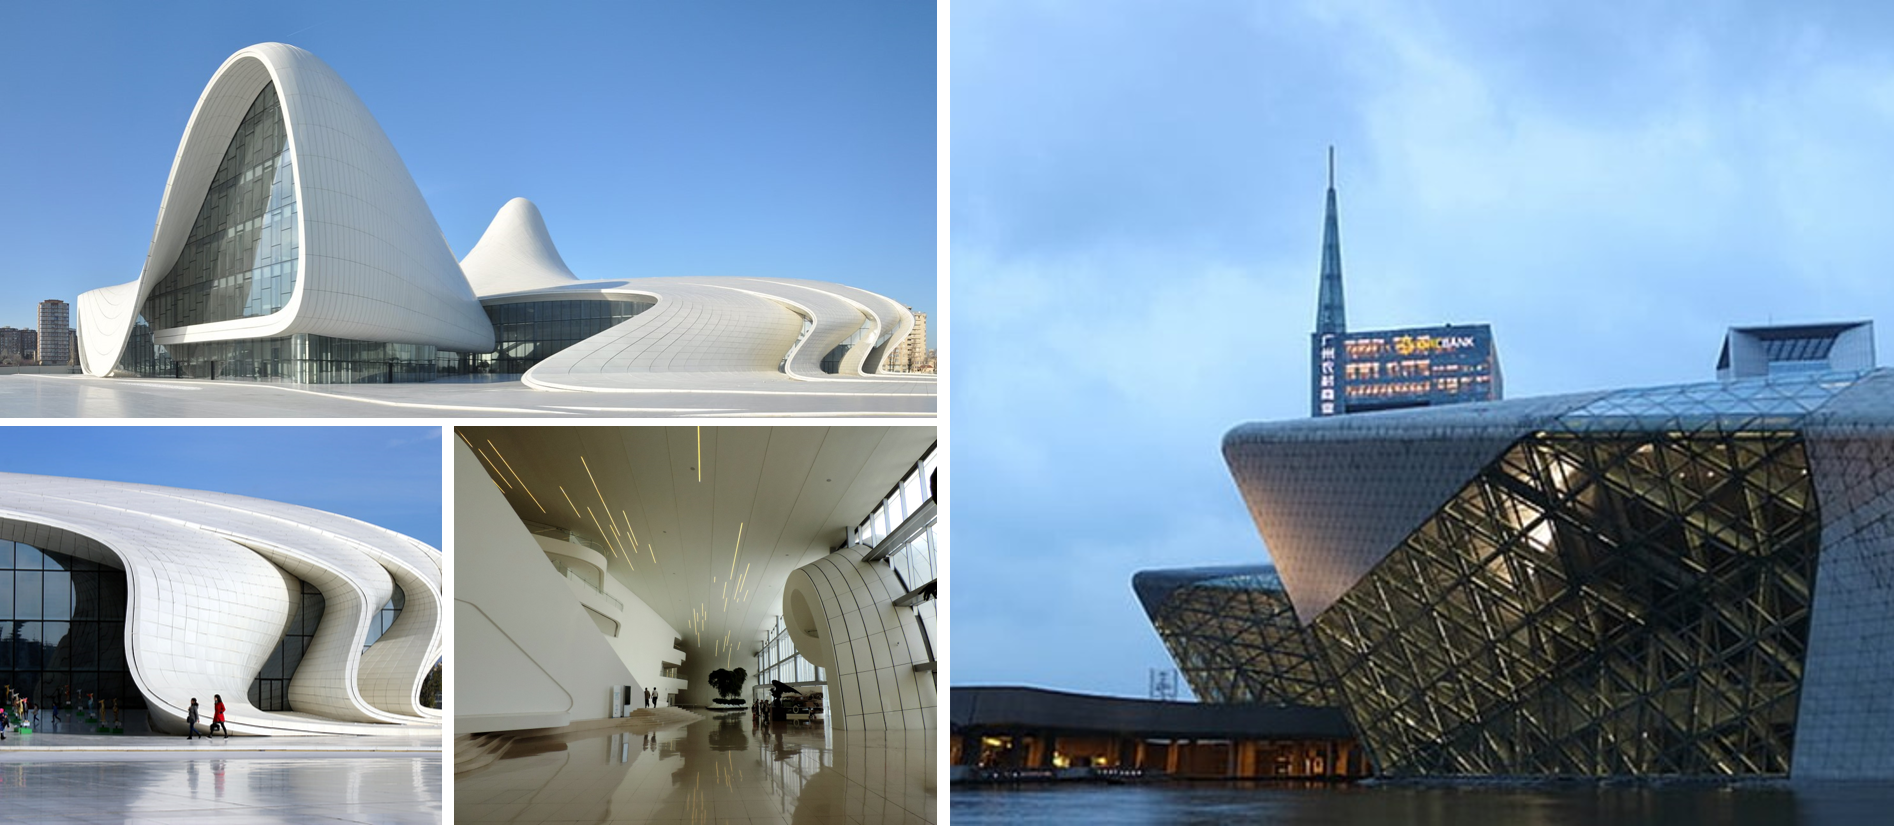
\includegraphics[width= \linewidth]{Images/Parametricism}
%          \caption{Parametricism approach to facades and ornament. (Left) Exterior and interior views of Heydar Aliyev Cultural Center, Baku, Azerbaijan, designed by Zaha Hadid, built in 2012. (Right) Guangzhou Opera House,  China, designed by Zaha Hadid, built in 2010. \textit{(Images edited from source)}}
%          \label{fig:Parametricism}
%        \end{figure}
%
%Parametricism leverages advanced computational tools to generate intricate and complex designs.
%In this architectural style, ornamentation often emerges algorithmically, with patterns and details that respond to specific parameters or input data.
%Through scripting, parametricism aims to differentiate and correlate all elements and subsystems of a design\cite{Schumacher2010}.
%
%These parametric ornaments are highly detailed and unique to each project, enhancing the building's identity while maintaining visual continuity with the overall design.
%
%To encapsulate, parametricism, as embodied by architects like Zaha Hadid,  stands as a transformative force in architectural design.
%Through the mastery of computational tools, it harnesses the power to create intricate and dynamic structures with emphasizes in the algorithmic generation of ornamentation, resulting in highly detailed and unique designs that encapsulate the spirit of innovation and complexity, pushing the boundaries of what architecture can achieve in the 21st century.
%
%%! Pragmatic utopianism
%
%Transitioning from parametricism to pragmatic utopianism, we encounter yet another intriguing architectural style that emerged in response to the evolving landscape of technology, sustainability, and design philosophy.
%
%While parametricism delves into intricate computational design and complex geometries, pragmatic utopianism embarks on a distinctive journey, combining functionality, sustainability, and a utopian vision for architecture and urban spaces.
%
%Pragmatic utopianism, is a concept denoting the fusion of an unrealistic ideal with a practical approach, resulting in an almost perfect representation of the world.
%Initially introduced by architect and bioregional planner Davidya Kasperzyk\cite{Stouhi2022}, is an architectural style that seeks to achieve an ideal world through designs that are grounded in reality (Figure\ref{fig:contemporarytimeline} \textit{e}).
%
%Bjarke Ingels and his firm, BIG, often embody this philosophy, as Ingels himself describes it as turning pure fiction into hard fact and surreal dreams into inhabitable space\cite{Ingels2015}.
%From the perspective of pragmatic utopianism, architecture should address pressing societal and environmental issues while also pushing the boundaries of innovation and aesthetics.
%
%Ingels' projects often feature sustainable elements seamlessly integrated into the design, addressing critical environmental concerns.
%For instance, the Amager Bakke plant combines waste management with a functional ski slope, ingeniously transforming a potential environmental problem into a recreational asset for the community.
%This project vividly exemplifies their commitment to the idea of interweaving public infrastructure with meaningful social programs\cite{Ingels2015} (Figure\ref{fig:Pragmaticutopianism}).
%
%%% Figure of pragmatic utopianism
%     \begin{figure}[t]
%          \centering
%          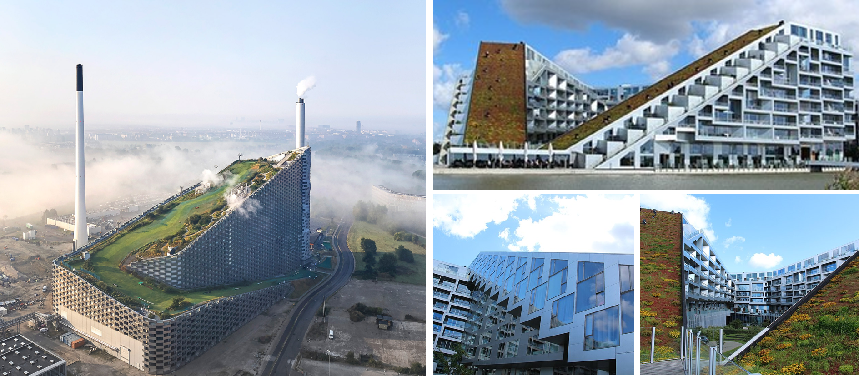
\includegraphics[width= \linewidth]{Images/pragmaticutopianism}
%          \caption{Pragmatic utopianism approach to facades and ornament. (Left) Amager Bakke, a waste-to-energy power station, Copenhagen, Denmark, design by BIG, built in 2019. (Right) 8 House, Copenhagen, Denmark, design by BIG, built in 2010. \textit{(Images edited from source)}}
%          \label{fig:Pragmaticutopianism}
%        \end{figure}
%
%This pragmatic utopian view emphasizes the role of architecture as a catalyst for positive change, both functionally and aesthetically, aiming to create a better future while responding to present needs .
%
%In terms of facades and ornamentation, pragmatic utopianism takes a minimalist yet purposeful approach.
%Facades are seen as not just aesthetic coverings but as functional interfaces, often a result of environmental analysis and parametric design that tailor the building envelopes to respond to different climate conditions\cite{Ingels2015}, having a crucial role in contributing positively to the environment and designed to be cost-effective and feasible, ensuring that the utopian vision is attainable within the constraints of the present.
%
%Ornamentation within the realm of pragmatic utopianism is inherently purpose-driven, rooted in functionality, sustainability, and a desire to convey the building's mission and its positive impact on society.
%It finds inspiration in the abstract art world and the imaginative realms of fictional films, where form and function harmoniously coexist\cite{Stouhi2022}.
%
%It embodies a subtle yet essential role, seamlessly integrated into the building's form.
%For instance, the graceful curves of the facade not only serve an aesthetic purpose but also communicate harmony with the nearby roadways.
%
%Green walls and vertical gardens are incorporated not just for their visual appeal but also for their substantial contributions to improved air quality and insulation.
%The facades often feature elements that cleverly serve dual functions, such as energy-efficient shading devices that simultaneously enhance the building's aesthetics.
%
%In summary, pragmatic utopianism, as seen through the works of Bjarke Ingels, embraces a holistic approach to architecture, combining ambitious visions with practical solutions, sustainability versed in environmental analysis, and meaningful ornamentation, that culminates in designs shaped by the forces that surround them, all while addressing the pressing challenges of our time.

%=============================
%edit the summary paragraph for pragmatic utopianism and add a conclusion that regards the advent of complexity

%“pragmatic utopia”, a utopia that combines an unattainable ideal with pragmatism, creating an almost ideal fragment of the world.
%First coined by architect and bioregional planner Davidya Kasperzyk, the term was further explored by Bjarke Ingles Group (BIG), describing an architectural style that pursues a perfect world through designs tempered by reality.\cite{Stouhi2022}

%turn surreal dreams into inhabitable space, to turn fiction into fact.\cite{Ingels2015}


%harness massive investments and imdue them with positive social side effect ... by proactively crossbreeding public infraestructure with social programs we can propagate new urban life-forms\cite{Ingels2015}

%The inability of post-modernism and deconstructivism to formulate a new viable paradigm led to the return of modernism in the guise of minimalism as the only consistent, ideologically stringent style that confronts parametricism today.\cite{Schumacher2010}


%Parametricism is the great new style after modernism.
%Postmodernism and Deconstructivism have been transitional episodes that ushered in this new, long wave of research and innovation \cite{Schumacher2008}.

%=============================



%establish bibliography references to defend the high tech section

% Continue writing the definition for the other styles after Deconstructivism

%Prominent contemporary architects such as Frank Gehry, Zaha Hadid, Bjarke Ingels, Santiago Calatrava, Renzo Piano, Norman Foster, and Herzog & de Meuron have contributed to the ongoing evolution of architectural expression, each bringing their distinctive approaches to facades and ornamentation.

%% add the transition to contemporary by simplifying the corntarst form modernism and post modernism like the reference from hopkins.

%% maybe add the ornament postmodernism image prepared on power point

%% Fix the ornamentation and facade descriptions with more concrete examples like do they use geometric lines colors or any specifics
%% prepare the transitioning towards the desconstructivism and revoultion of the late

    %Venturi's stance championed a departure from rigid conformity and highlighted the richness that emerges from embracing the complexities of the human experience and the interconnectedness of design with its cultural, historical, and contextual underpinnings.

%% reorganize the venturi text and seprate it from the critic of modernism. Add a las vegas analyses pic or something related to the soulless architecture. revision the interpretation of facades and ornament with citations before progressing into the contemporary

%%i need to add a paralel that our cities were generated under the modernist ideals and preference of the car which lead to the reference to Las vegas and how if you remove the signs, there is no place only a desert due to the disengage of architecture now reduce to a cheap necessity hidden behind the sign. Also add a picture of the postmodern style with a reference towards facade and ornament made clear in similar fashion as the conclusions of style written before that ussually start with in essence.

%I want to make a reflection at this point, the modernist movement utopia failed and resulted in the creation of monotonous places desensatized from its culture.
%the functionalism was misinterpreted as plainliness and resulted in dehumanized elements.
%the focus on light and glass facades ignored contextual relationship where the climate unapologetically would turn this glass boxes into ovens pradoxical ignoring the maxim of human centric design.
%architecture would follow a pattern regardless of its roots and connection to its local making them virtually indistinguishable from one another in striking contrast to the richful global diversity of the past.
%the absence of ornament was misinterpreted as the lack of effort reducing architecture to mere construction.

   %%%==========================References




    %\subsection{Digital fabrication and Environmental Sustainability}
    %\label{subsec:DigitalFabricationAndEnvSustainability}
    %
%\subsection{Digital fabrication and Environmental Sustainability}
%\label{subsec:DigitalFabricationAndEnvSustainability}

%==========================
%8. **Environmental Sustainability:** Investigate how the integration of complex facades and digital fabrication aligns with contemporary sustainability principles. Examine how parametric design and data-driven approaches can enhance energy efficiency, reduce material waste, and contribute to sustainable construction practices.
%==========================

Digital fabrication technologies, meanwhile, are interacting with the biological world on a daily basis.
Engineers, designers, and architects are combining computational design, additive manufacturing, materials engineering, and synthetic biology to pioneer a symbiosis between microorganisms, our bodies, the products we consume, and even the buildings we inhabit\cite{Schwab2016}.


 If articulation has taken over from ornament in the architecture of abstract expressionism, space is what displaced symbolism: space dramatized by an acrobatic use of light. Our heroic and original symbols, from carceri to Cape Kennedy, feed our late Romantic egos and satisfy our need for spectacular, expressionistic space for a new age in architecture. To day, however, most buildings need reasonably low ceilings and windows rather than glass walls for light, to contain the air conditioning and meet the budget. Therefore our esthetic impact should come from sources other than light and space, more symbolic and less spatial sources\cite{}


    %!% Figures Methodology intro
    %% Methodology Flowchart
    \begin{figure*}[!htb]
        \centering
        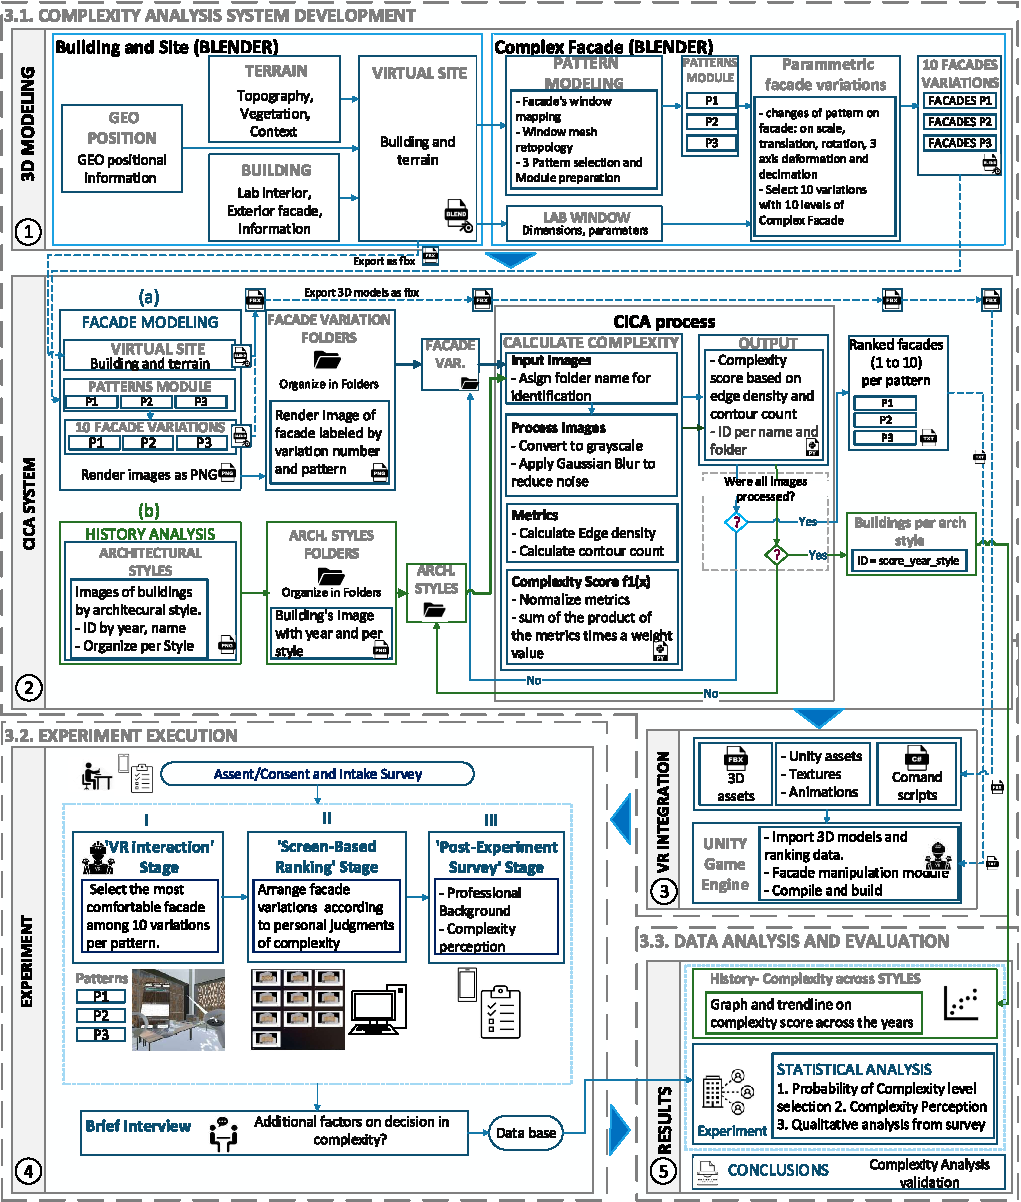
\includegraphics[width=\linewidth]{Images/MethodologyFlowchart}~\caption{Methodology Flowchart illustrating the sequential steps of this study's approach framework designed to assess the qunatification of complexity in building design and the perception of occupants in complex environemnts. Higlighting the usage of the CICA system (element 2) (detailed in Section~\ref{subsubsec:CICAsystem}) in the Complexity Analysis System development (detailed in Section\ref{subsec:ComplexitySystemDevelopment}), and the transition to `Experiment Execution' (element 4) (described in Section\ref{subsec:Experiment_execution}), culminating in the post-experiment data analysis and results phase (element 5) (described in Section\ref{subsec:Data_analysis}).}
          \label{fig:MethodologyFlowchartComplexity}
    \end{figure*}


\section{Methodology}
\label{sec:Methodology}
%%Methodology
%%methodology Intro


The methodology of this study, comprises three main components (subdivided into 5 key steps, as illustrated in  Figure~\ref{fig:MethodologyFlowchartComplexity}):

\begin{enumerate}
    \item \textit{Complexity Analysis System Development:} Outlined in Section~\ref{subsec:ComplexitySystemDevelopment} (Figure~\ref{fig:MethodologyFlowchartComplexity}, element 3.1), this component integrates a VR framework with the CICA system.~The CICA system uses CV algorithms to quantitatively assess facade design complexity, applied to both contemporary 3D-modeled facades and historical analysis.~The VR component allows real-time participant interaction with facade variations, combining 3D models and CICA analysis. Key elements include the 3D modeling process (Section~\ref{subsubsec:3DModeling}, Figure~\ref{fig:modeling_flowchart}), the CICA system (Section~\ref{subsubsec:CICAsystem}, Figure~\ref{fig:CICA_and_VR_flowchart}), and VR integration (Section~\ref{subsubsec:VR_integration}, Figure~\ref{fig:CICA_and_VR_flowchart}).

    \item \textit{Experiment Execution:} Detailed in Section~\ref{subsec:Experiment_execution} (Figure~\ref{fig:MethodologyFlowchartComplexity}, element 3.2), this phase involves participants engaging with the `Complexity Analysis' system through three stages: `VR Interaction' Stage, `Screen-Based Ranking' Stage, and `Post-Experiment Survey'. This process combines quantitative CICA scores and qualitative user feedback.

    \item \textit{Data Analysis and Validation:} Detailed in Section~\ref{subsec:Data_analysis} (Figure~\ref{fig:MethodologyFlowchartComplexity}, element 3.3), this final component analyzes both CICA scores and experiment data to validate the system’s effectiveness in measuring complexity and user preferences. Statistical tools are used to evaluate the alignment between CICA scores and user perceptions. The system's accuracy and its application to historical and contemporary facades are assessed through detailed complexity analysis, providing insights for architectural design practices.
\end{enumerate}

With the methodology outlined, we now move forward to a comprehensive breakdown of each component.

%\textbf{CICA system:} Detailed in Section~\ref{subsec:CICAsystem} and depicted as (3.1) in Figure~\ref{fig:MethodologyFlowchart}, involves developing a Python script using computer vision algorithms to process images and yield complexity scores, quantitatively gauging the intricacy of architectural designs.
%It supports theoretical analyses and provides a ranking framework for facade designs in the VR system.
%
%\textbf{VR System Development:}  Outlined in Section~\ref{subsec:VRsystemDevelopment} and represented as (3.2) in Figure~\ref{fig:MethodologyFlowchart}, this component focuses on creating an immersive experience where participants can explore and interact with a building's interior and exterior, manipulating facade designs with variable complexity levels and experiencing their impact.
%
%\textbf{Experiment Execution:} Detailed in Section~\ref{subsec:Experiment_execution} and illustrated as (3.3) in Figure~\ref{fig:MethodologyFlowchart}, following a similar approach to previous studies~\cite{Wolfartsberger2019}, this component outlines the method to evaluate users' acceptance of building complexity.
%It consists of three stages: a VR interaction stage, a screen-based stage, and a post-interaction survey.
%These stages allow for the collection of quantitative and qualitative data on participants' perceptions and responses to different complexity levels in facade designs.
%
%As illustrated in the methodology flowchart (Figure~\ref{fig:MethodologyFlowchart}), these components are combined to integrate computational analysis with immersive VR experiments, exploring user preferences in facade design and providing insights into architectural trends.
%
%With this methodology outlined, the following sections will now delve into a comprehensive breakdown of each component, highlighting their objectives, methodologies, and significance in achieving our research goals.

%!Figures Modeling
    %Figure Real vs 3d Model
    \begin{table*}[!htb]
    \centering
    \small
    \begin{tabular}{c}
        %Top cell with one figure
        %Figure Real vs 3d Model
        \begin{minipage}{\textwidth}
        \centering
        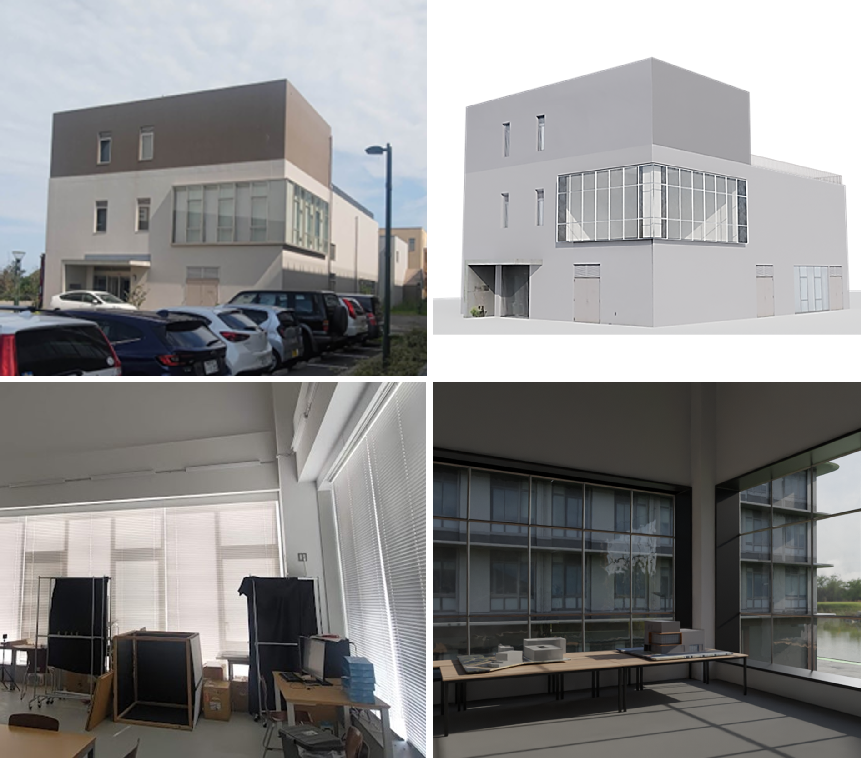
\includegraphics[width= \linewidth]{Images/Realvs3DmodelBlender}
                    \captionof{figure}{Comparison side by side of the actual Architectural Environment Building exterior (a) and interior (c) with its detailed 3D virtual clone counterpart (b, d) created for the VR experiment for Facade complexity Analysis, demonstrating the fidelity of the digital model in replicating architectural nuances.}
                    \label{fig:RealVs3dModel}
        \end{minipage}
        \\
        \\
        \\
        %Bottom cell
        %Table: Table: Pattern Variations sample 1, 7, 9
        \begin{minipage}{\textwidth}
            \centering
            \captionof{table}{Table of Facade Pattern Variations: This table presents samples of 3D-modeled building facades at levels 1, 3, and 9, showcasing the progression and differentiation within the ten facade variations as detailed in section~\ref{subsubsec:3DModeling}. The incremental complexity introduced at each selected variation is highlighted across three distinct patterns. For a comprehensive record of all variations, refer to~\ref{sec:AnnexVariations}.}
            \label{tab:PatternsVariationsPart0}
            \begin{tabularx}
            {\textwidth}{p{3cm} >{\centering\arraybackslash}X >{\centering\arraybackslash}X >{\centering\arraybackslash}X }
        \toprule
        \multicolumn{4}{c}{\textbf{Progression of 3D-Modeled Facade Variations Across Patterns: A Comparative Analysis at Levels 1, 3, and 9}}\\
        \toprule
        \textit{Description} &
          \textit{Pattern 1} &
          \textit{Pattern 2} &
          \textit{Pattern 3} \\
        \midrule
        \text{Pattern Name} & Hishi Pattern & Tortoise shells & Asanoha Pattern\\

        \midrule
        \textit{Base Module} &  &  &
        \\
        {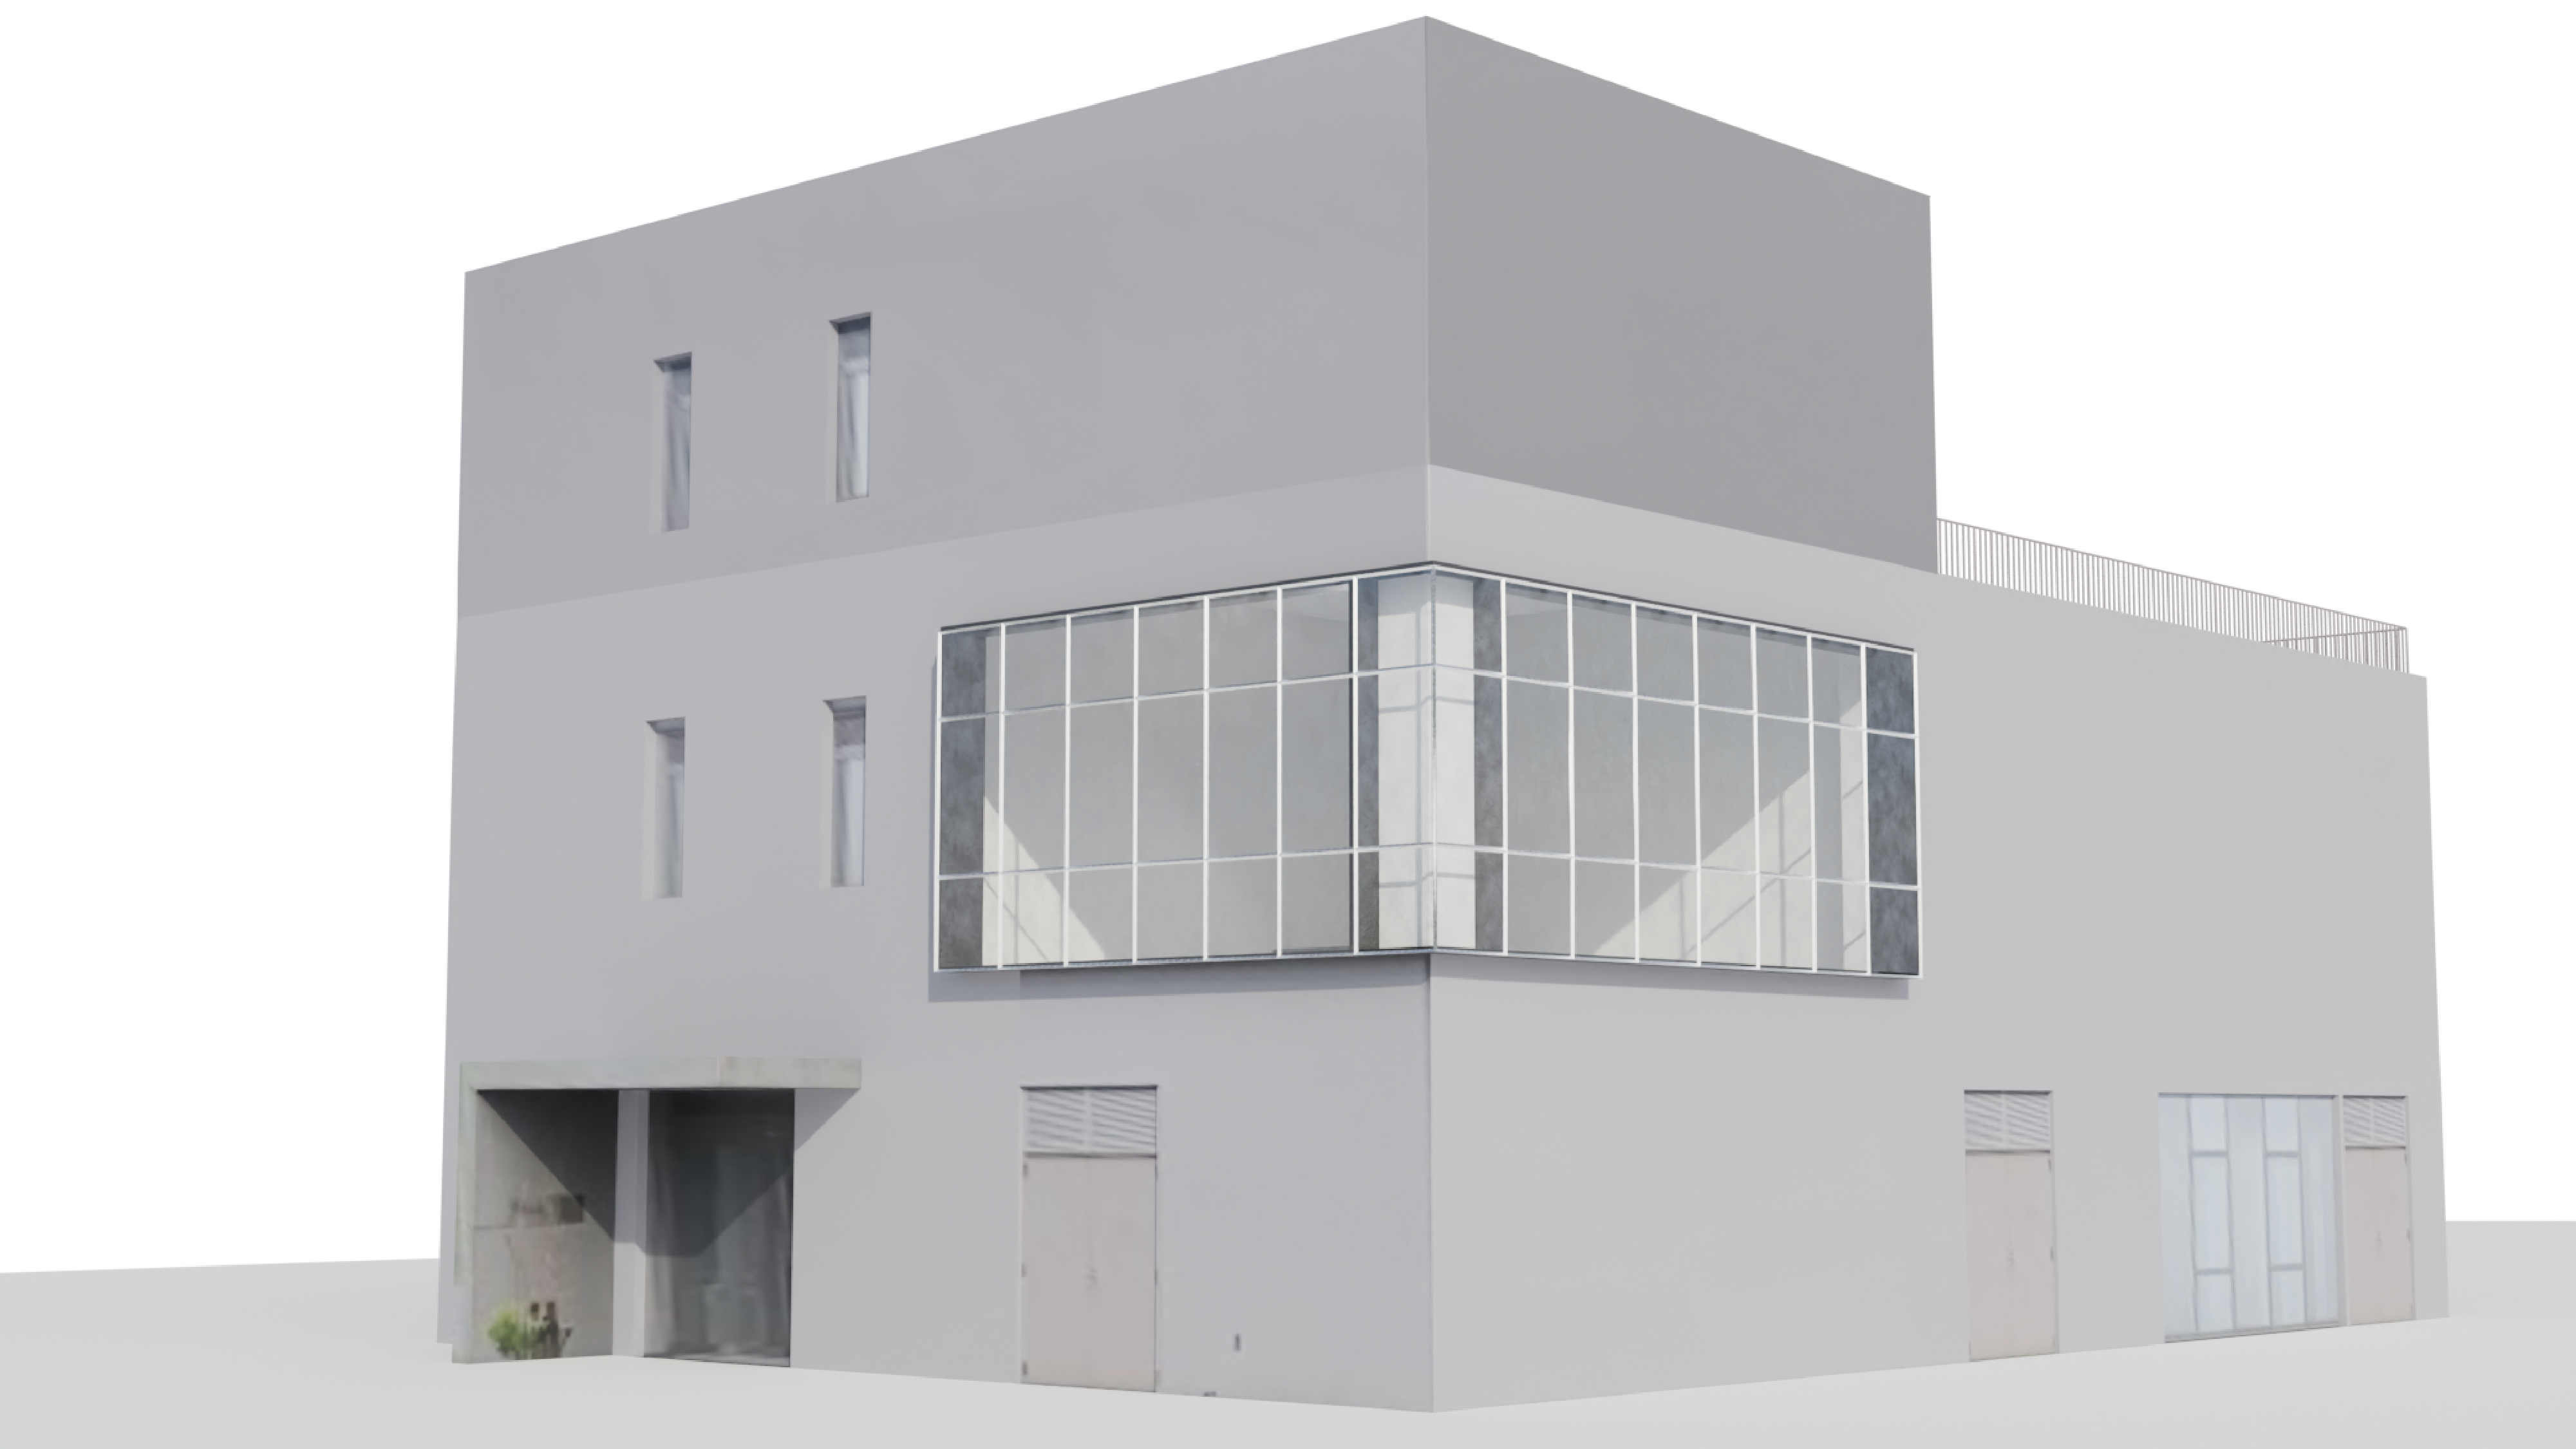
\includegraphics[width=1\linewidth]{Images/Base Module/Building}} &
          {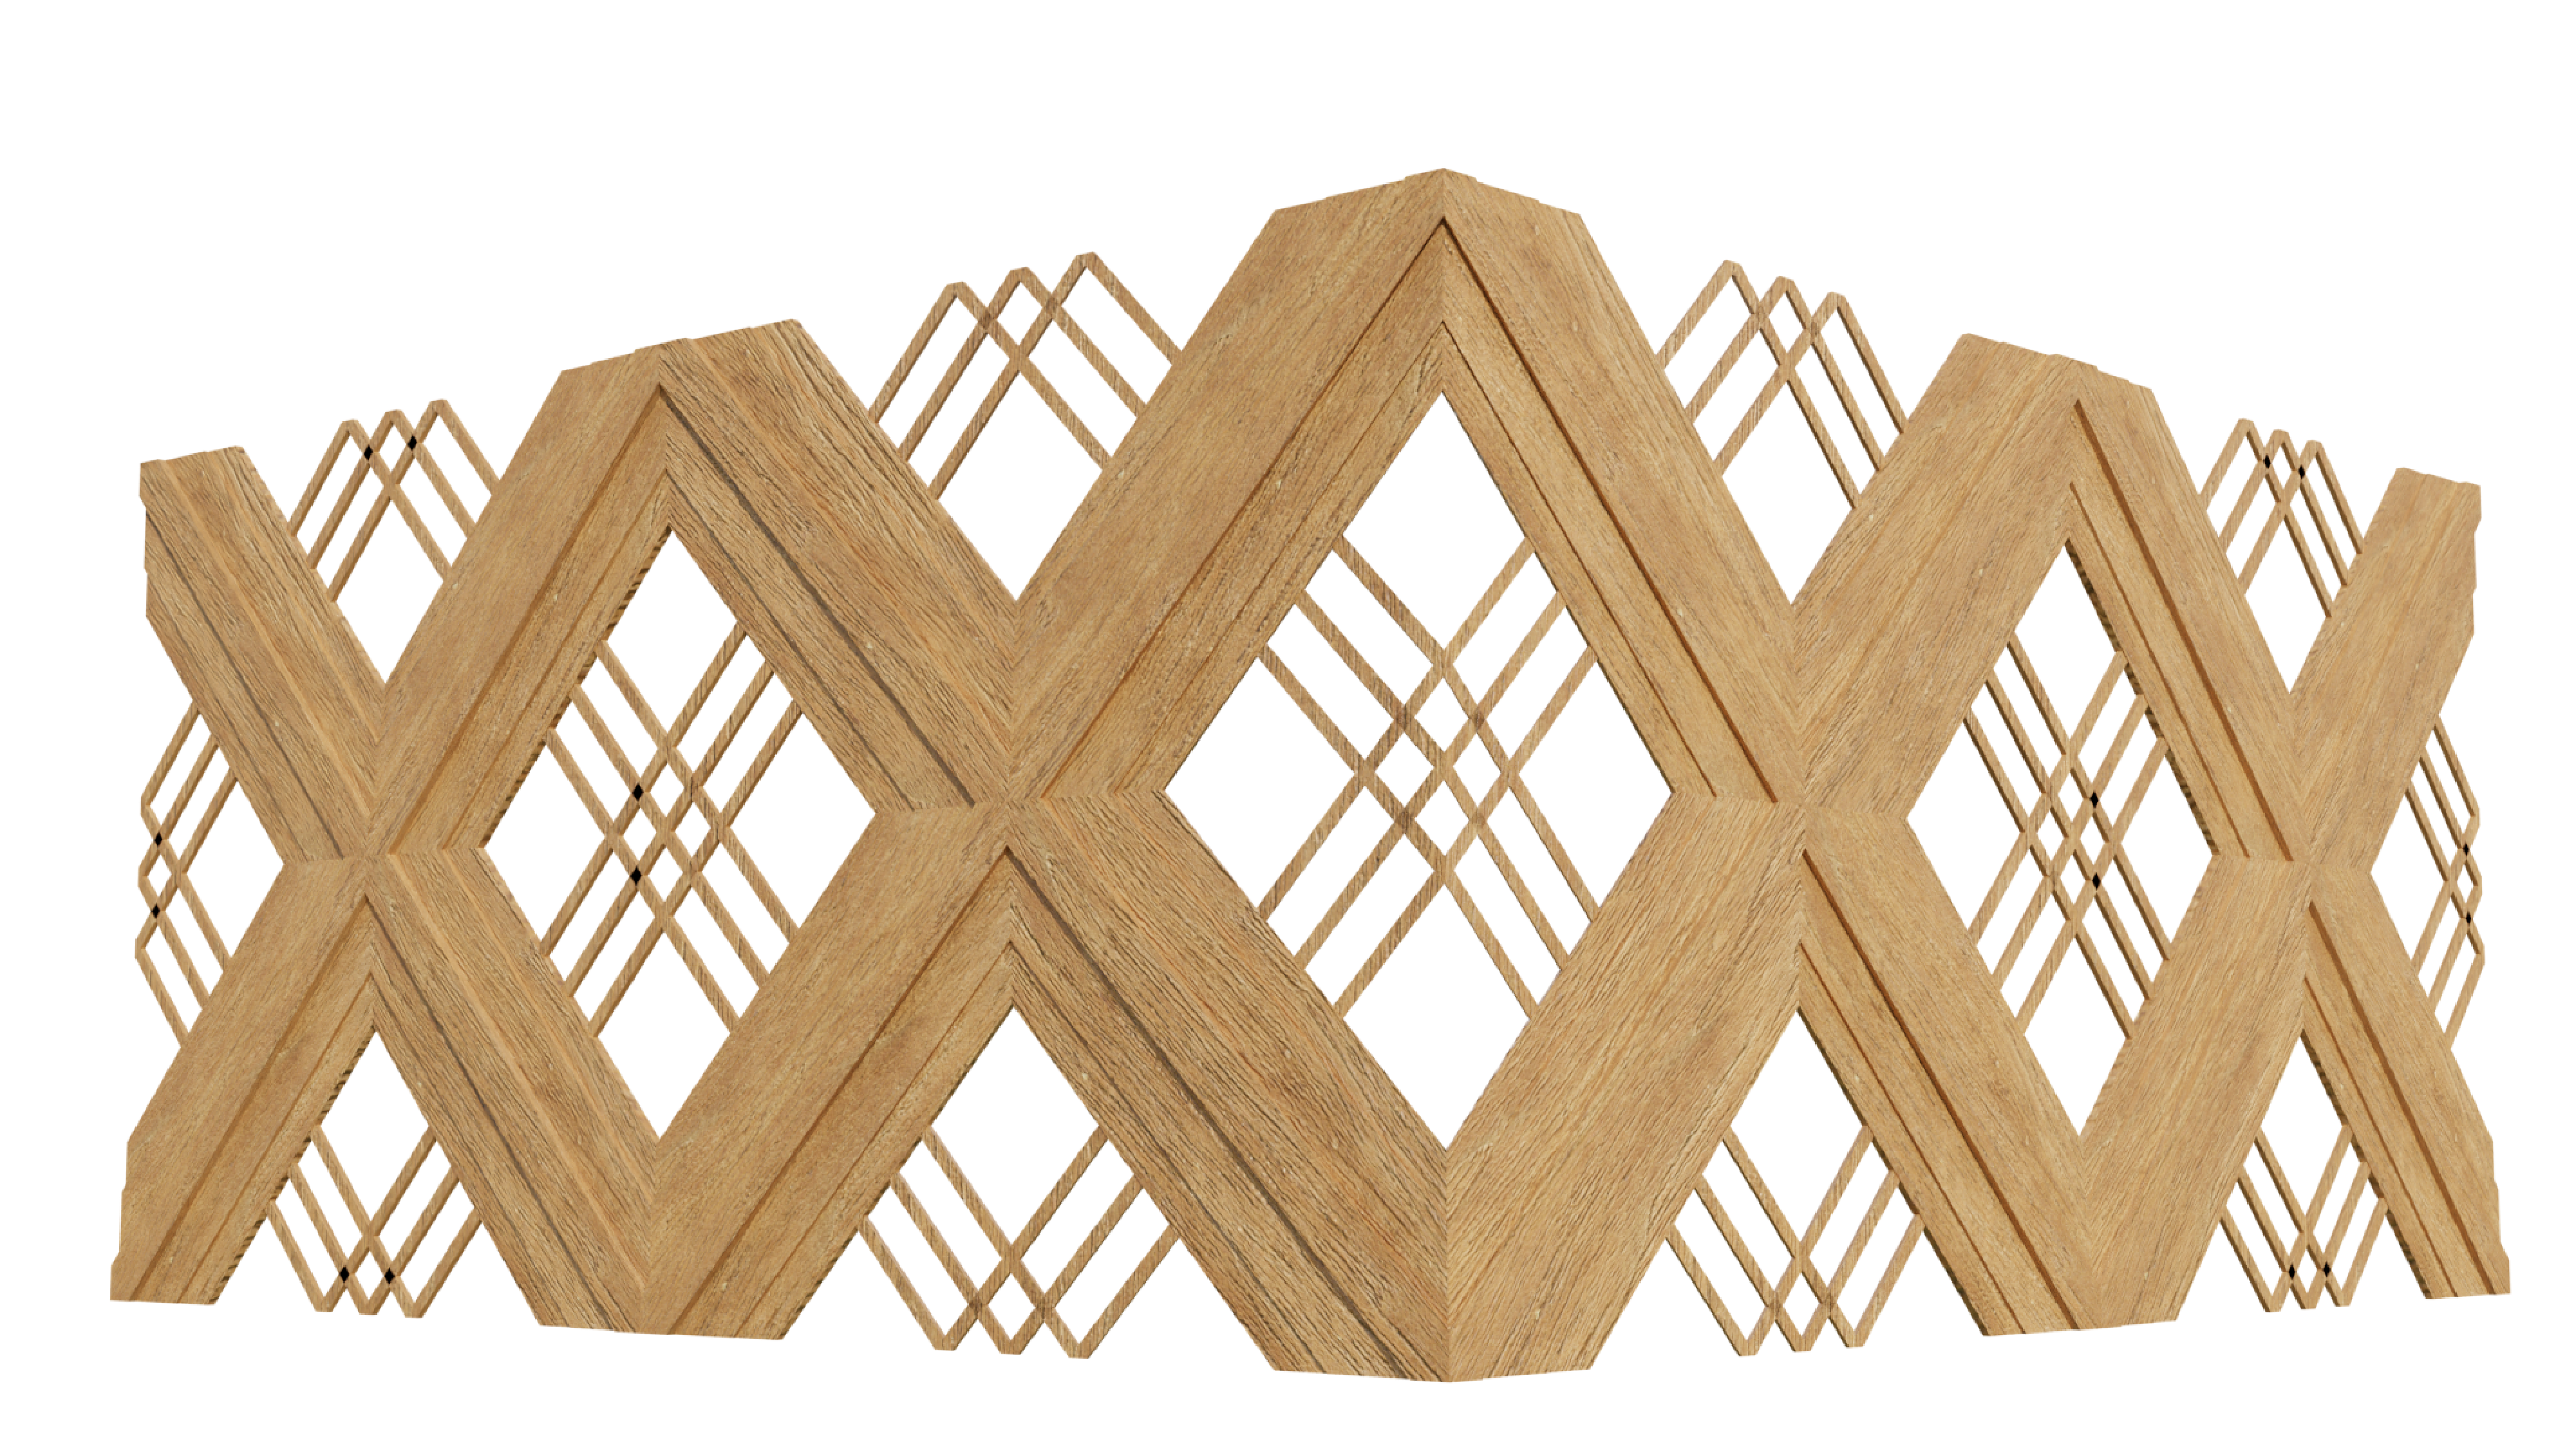
\includegraphics[width=1\linewidth]{Images/Base Module/Pattern1}} &
          {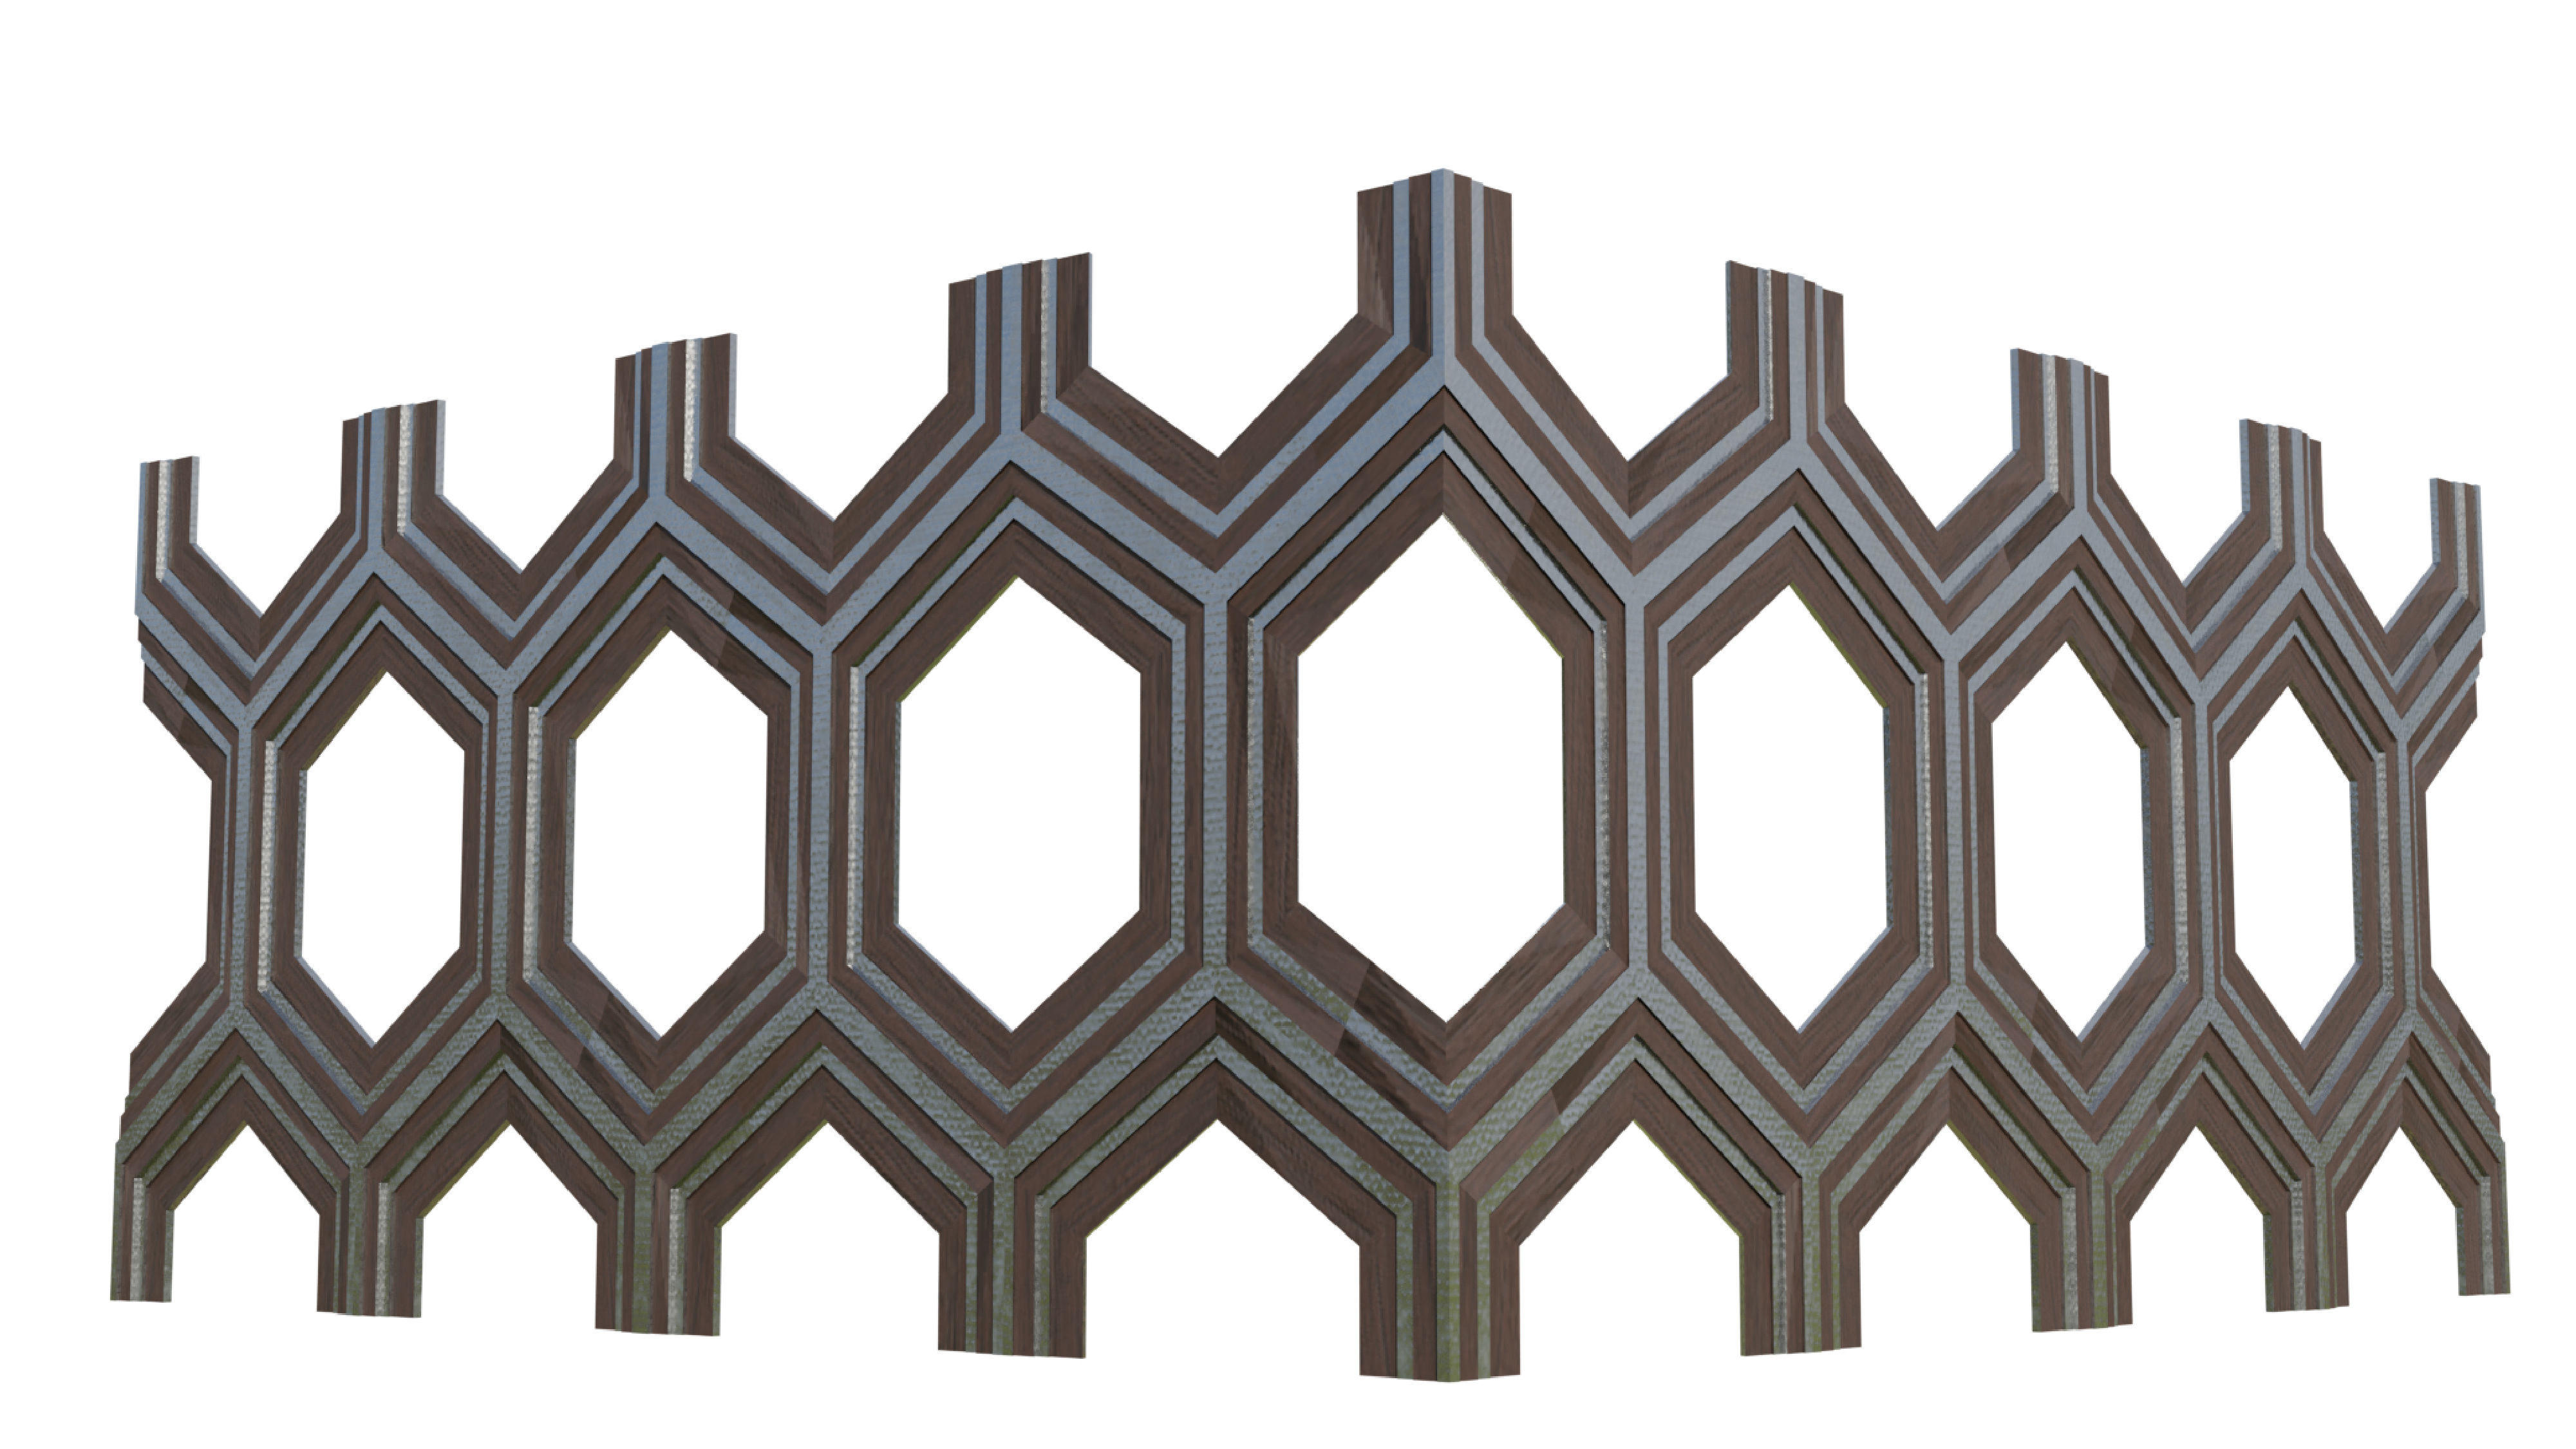
\includegraphics[width=1\linewidth]{Images/Base Module/Pattern2}} &
          {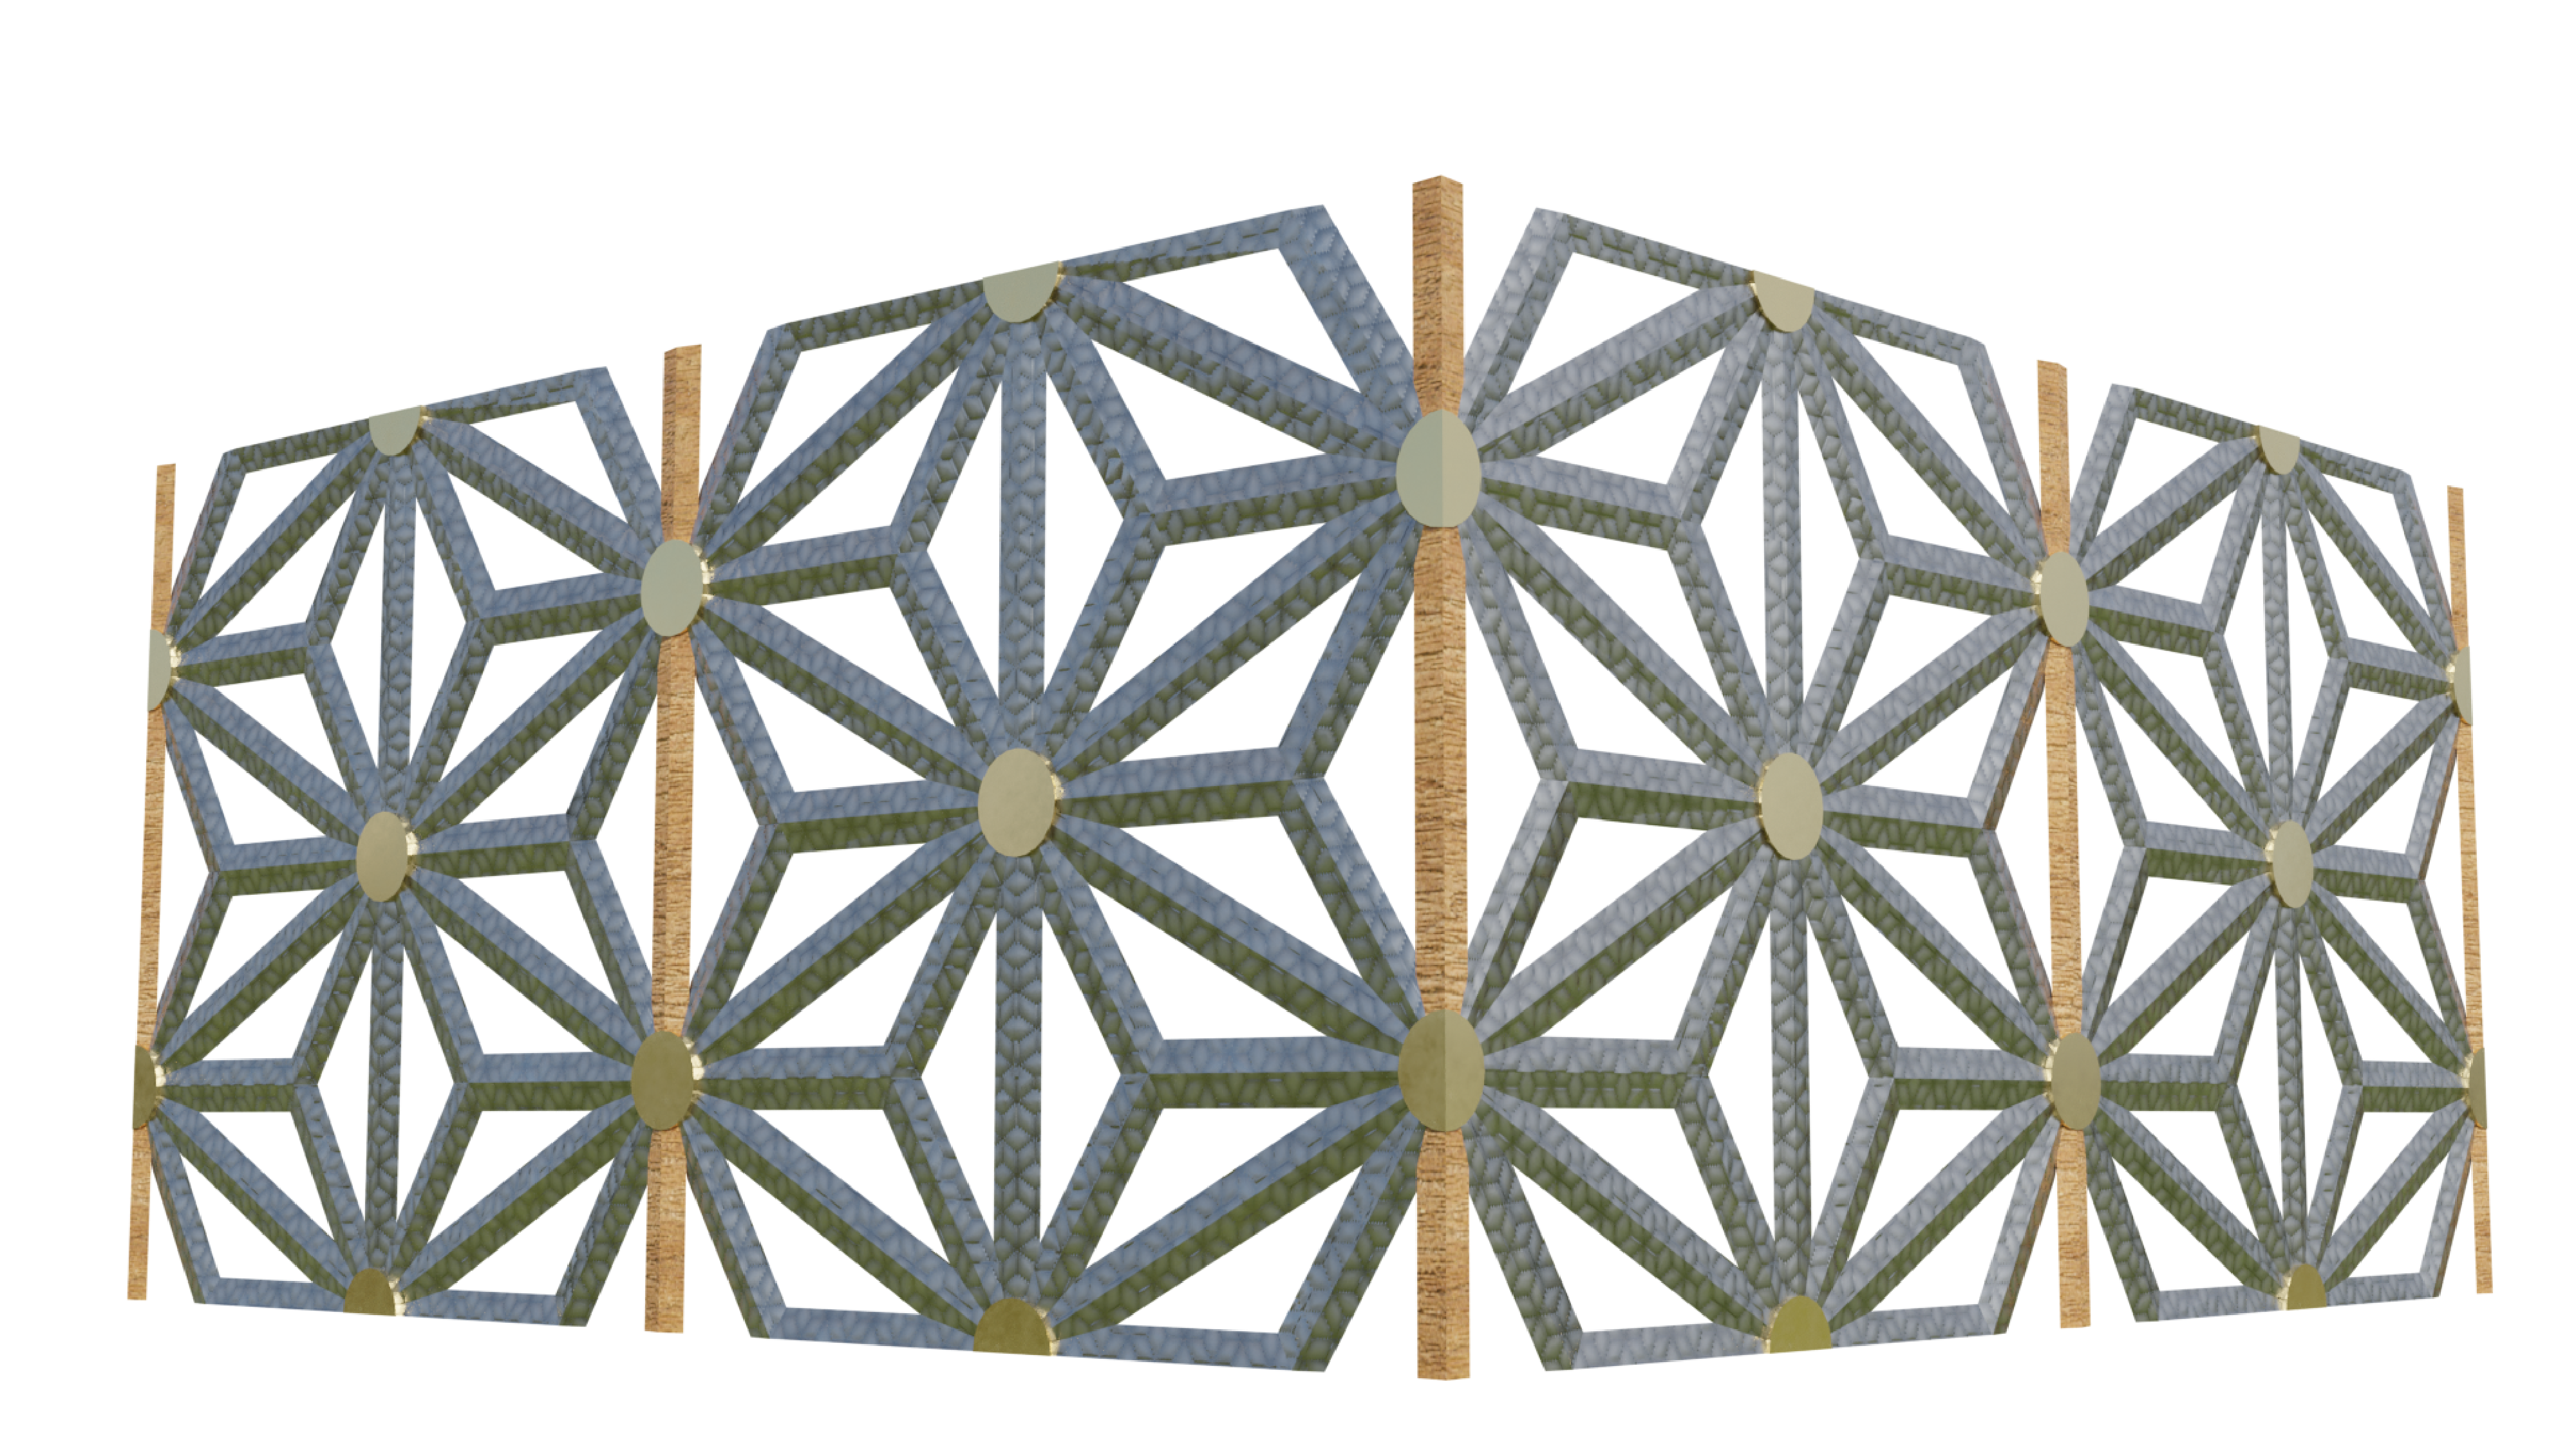
\includegraphics[width=1\linewidth]{Images/Base Module/Pattern3}} \\
        \midrule

        \textit{Mesh complexity Level} &
          \textit{Pattern 1} &
          \textit{Pattern 2} &
          \textit{Pattern 3}\\

        \midrule
        \textit{Level 1} &  &  &
        \\
        {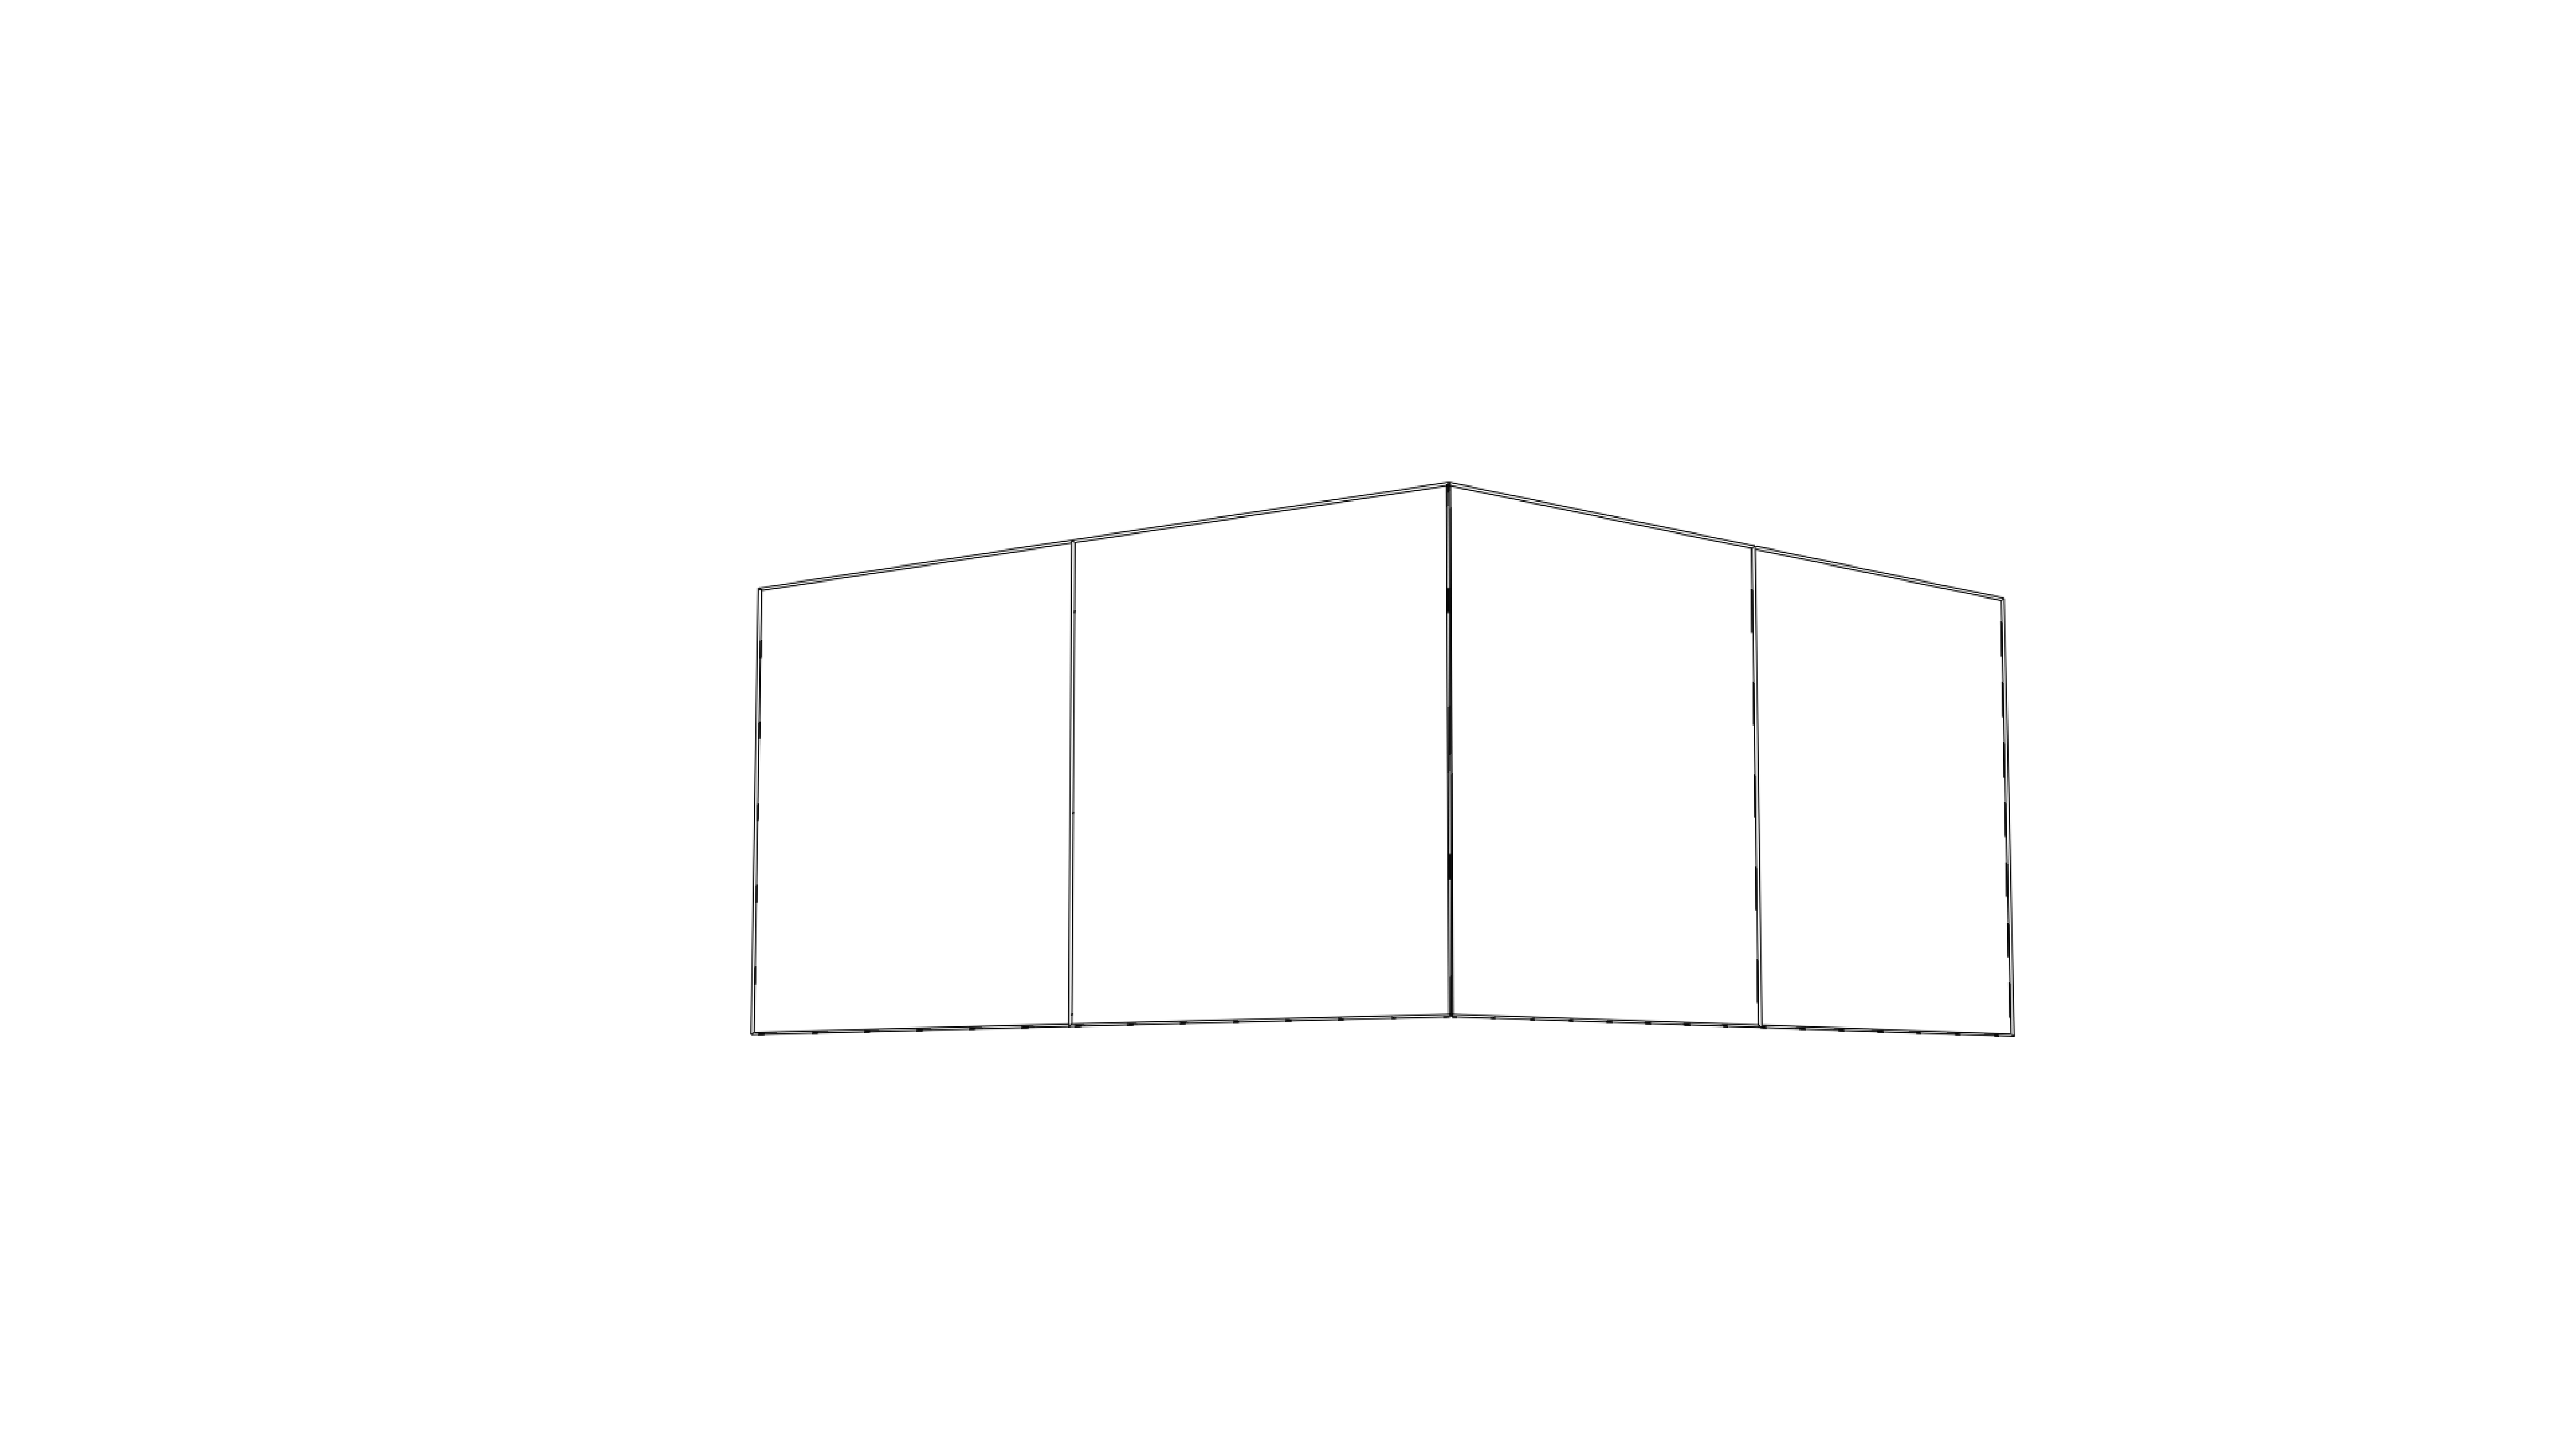
\includegraphics[width=1\linewidth]{Images/Wall 0/0001}} &
            {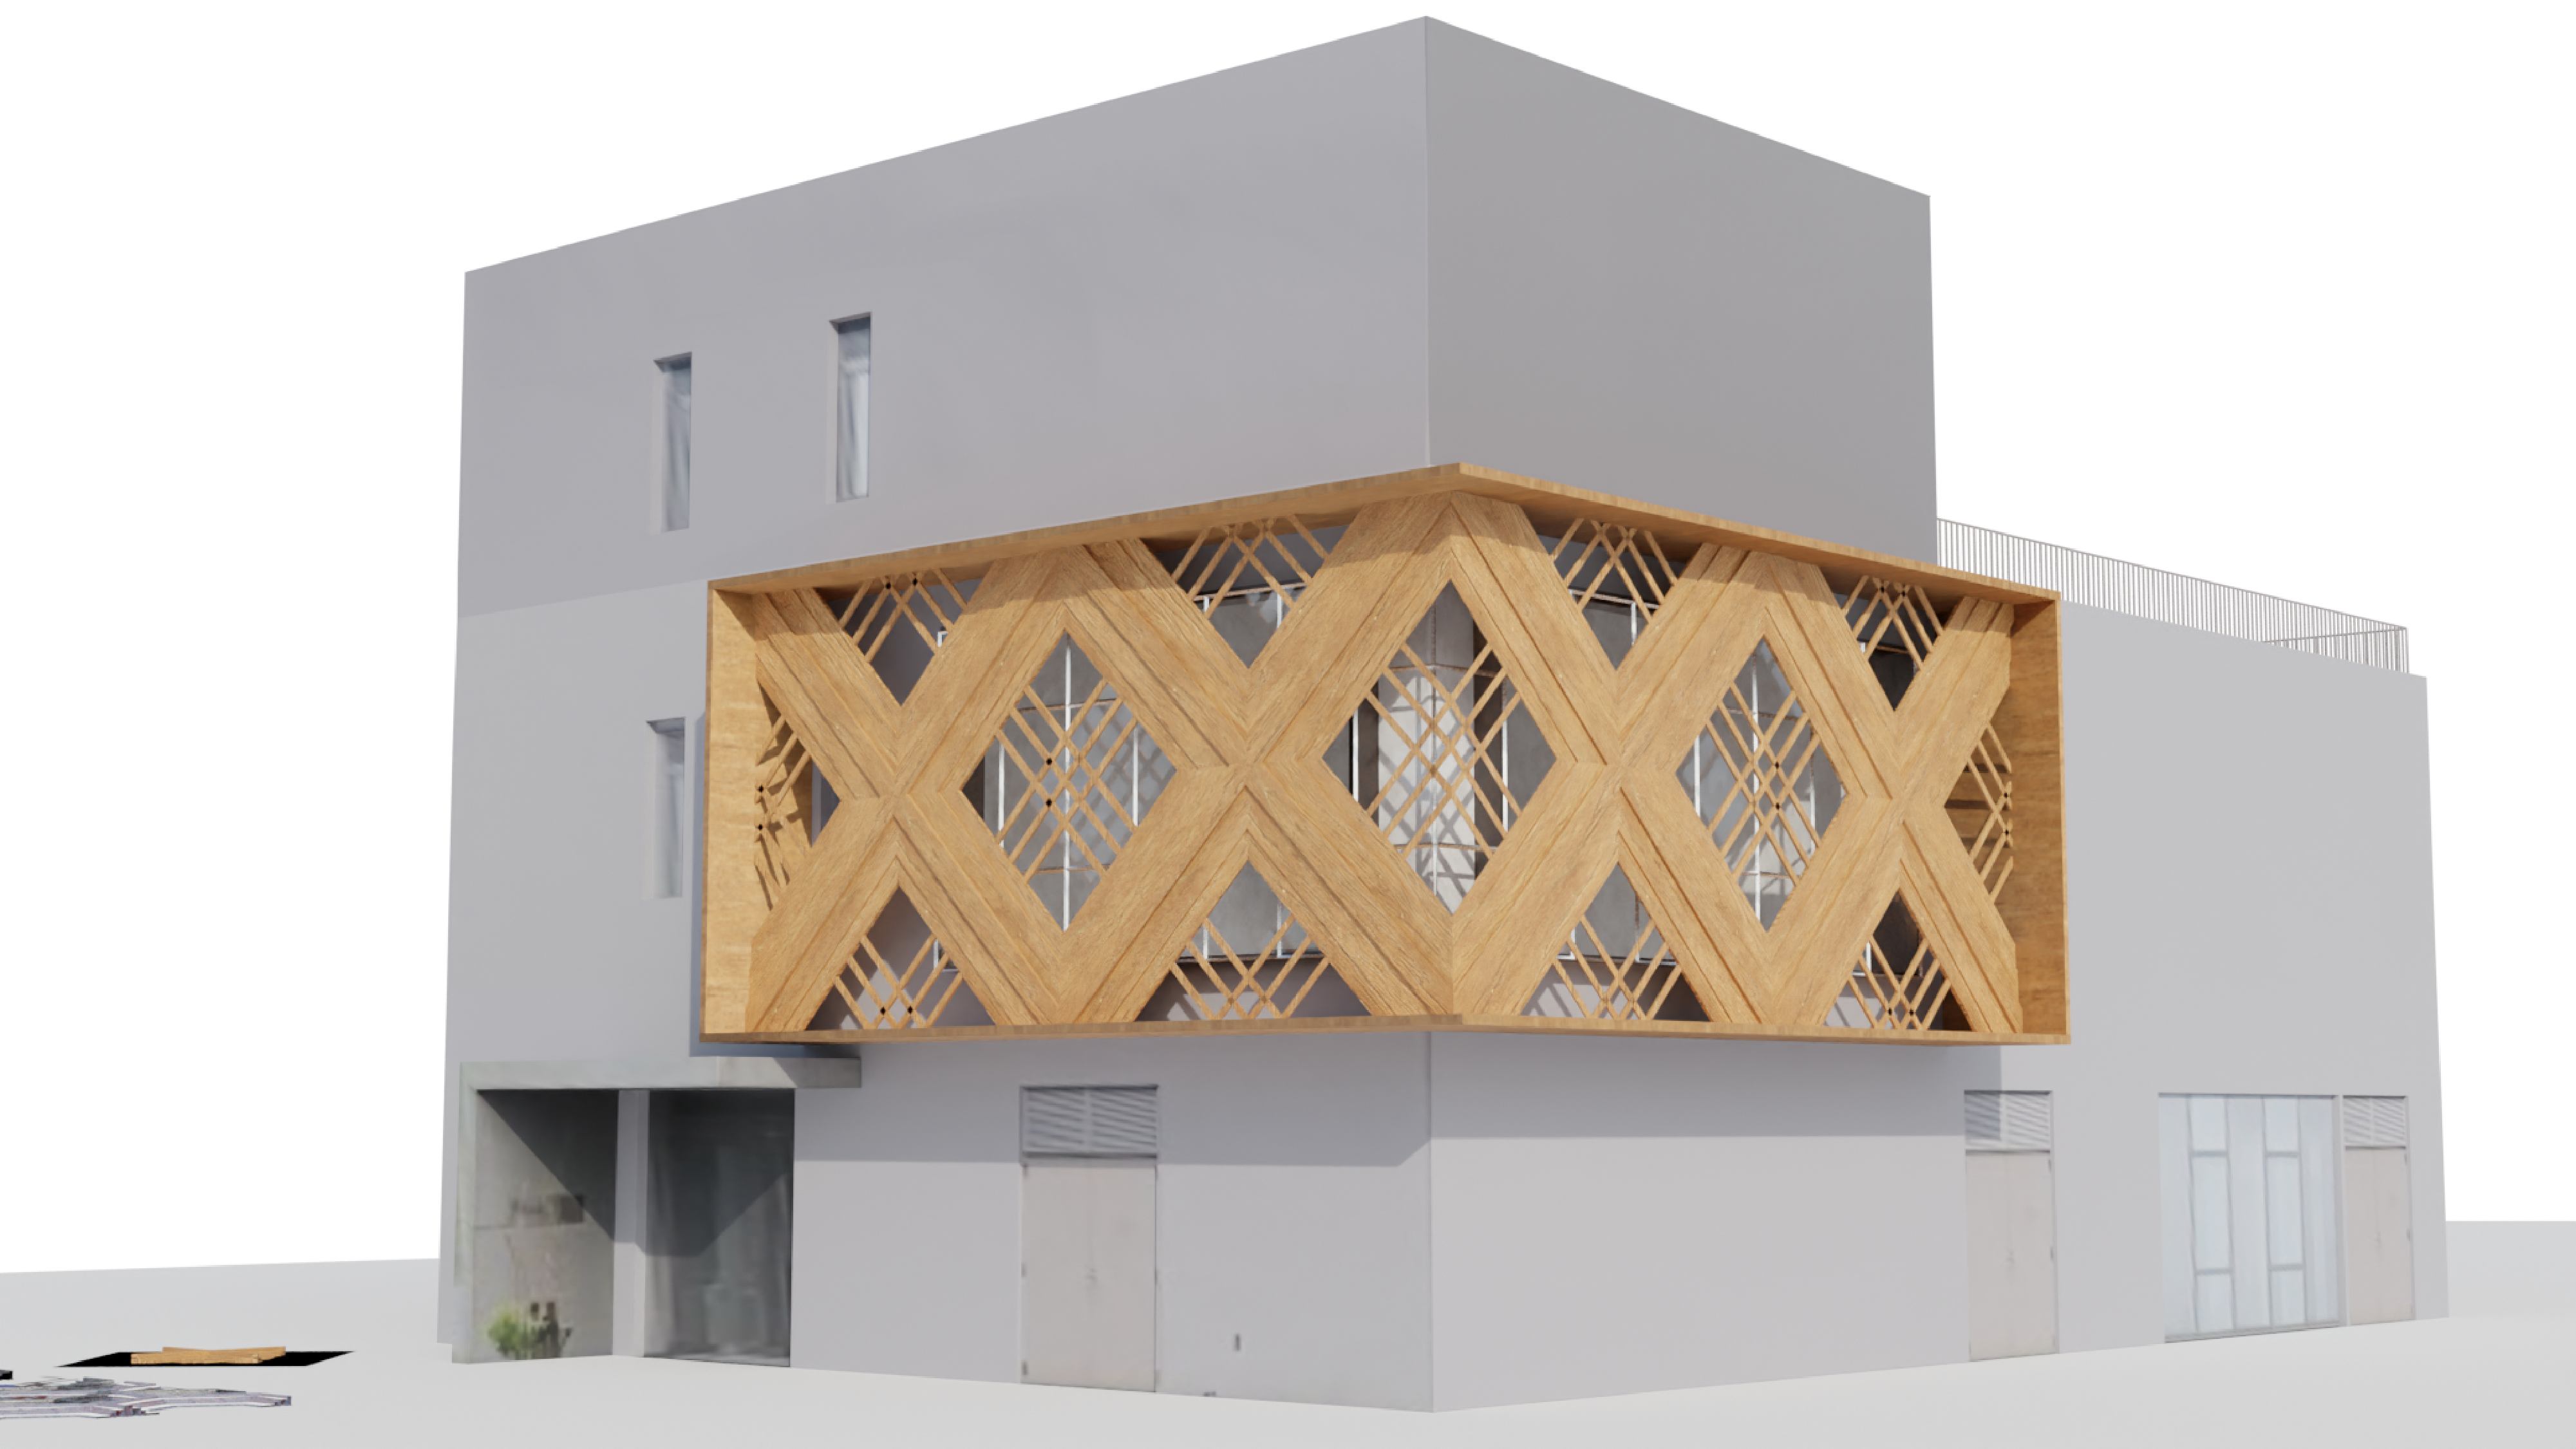
\includegraphics[width=1\linewidth]{Images/Pattern 1/0001}} &
          {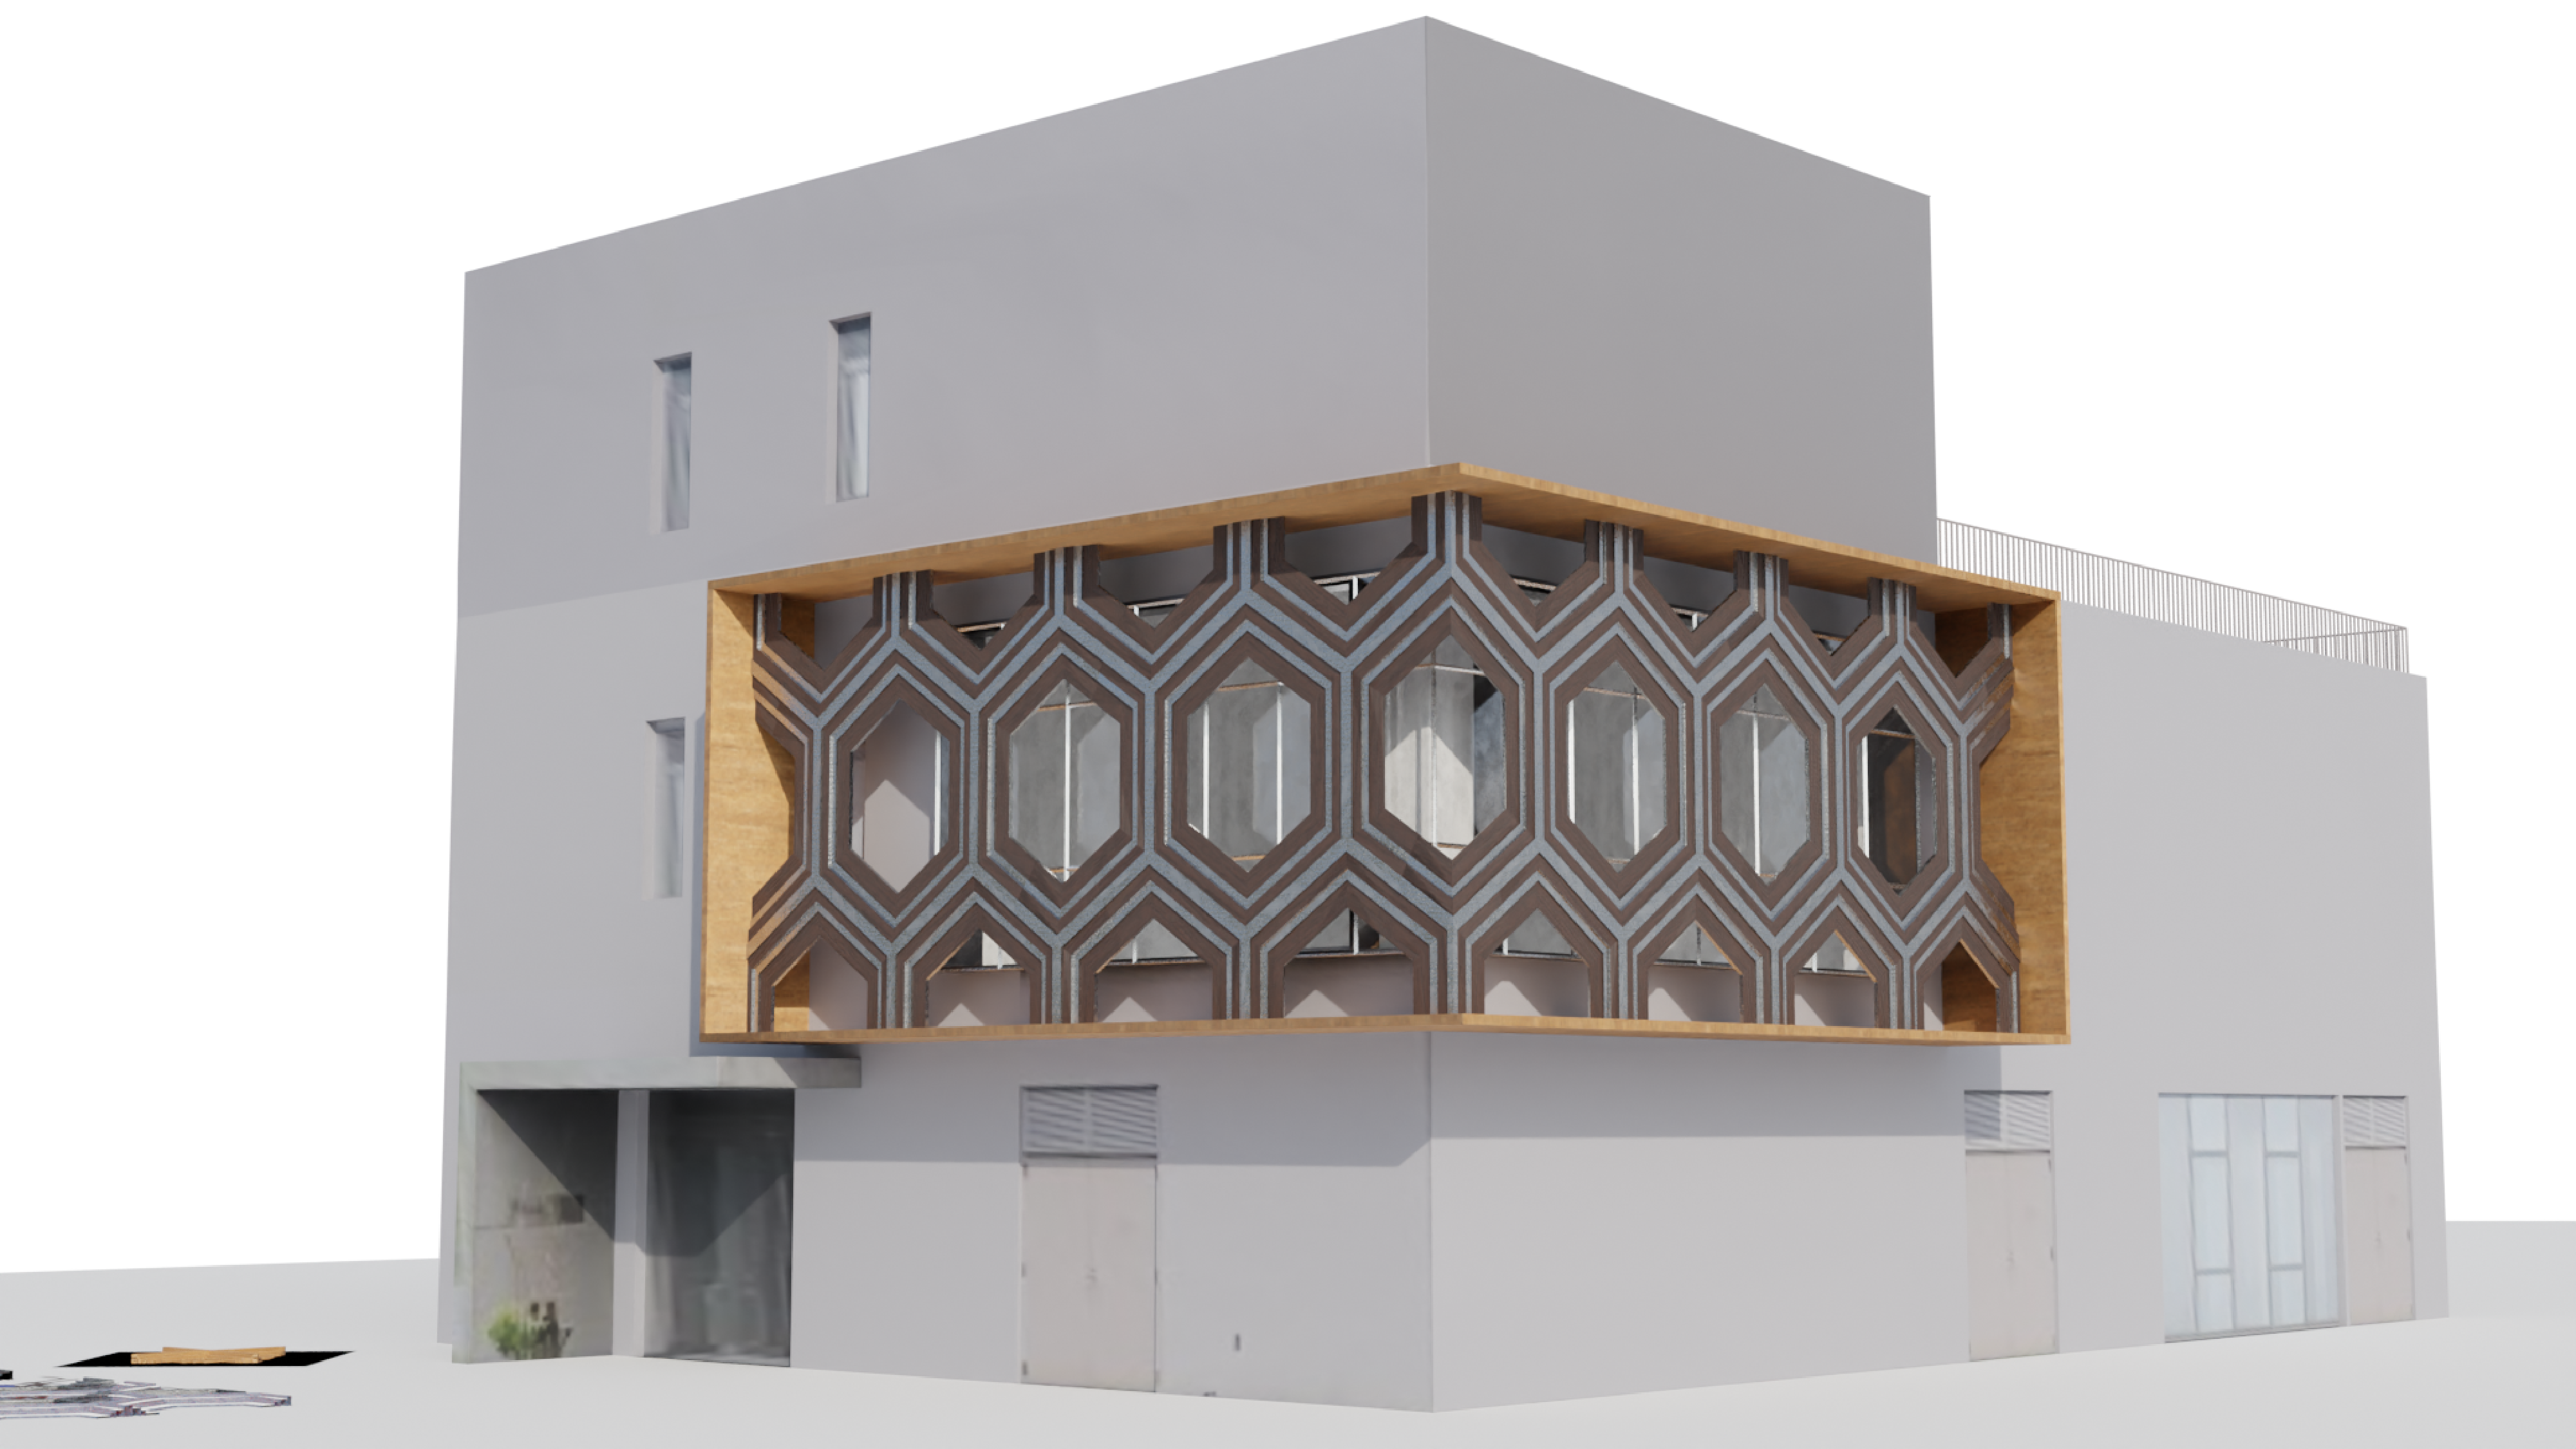
\includegraphics[width=1\linewidth]{Images/Pattern 2/0001}} &
          {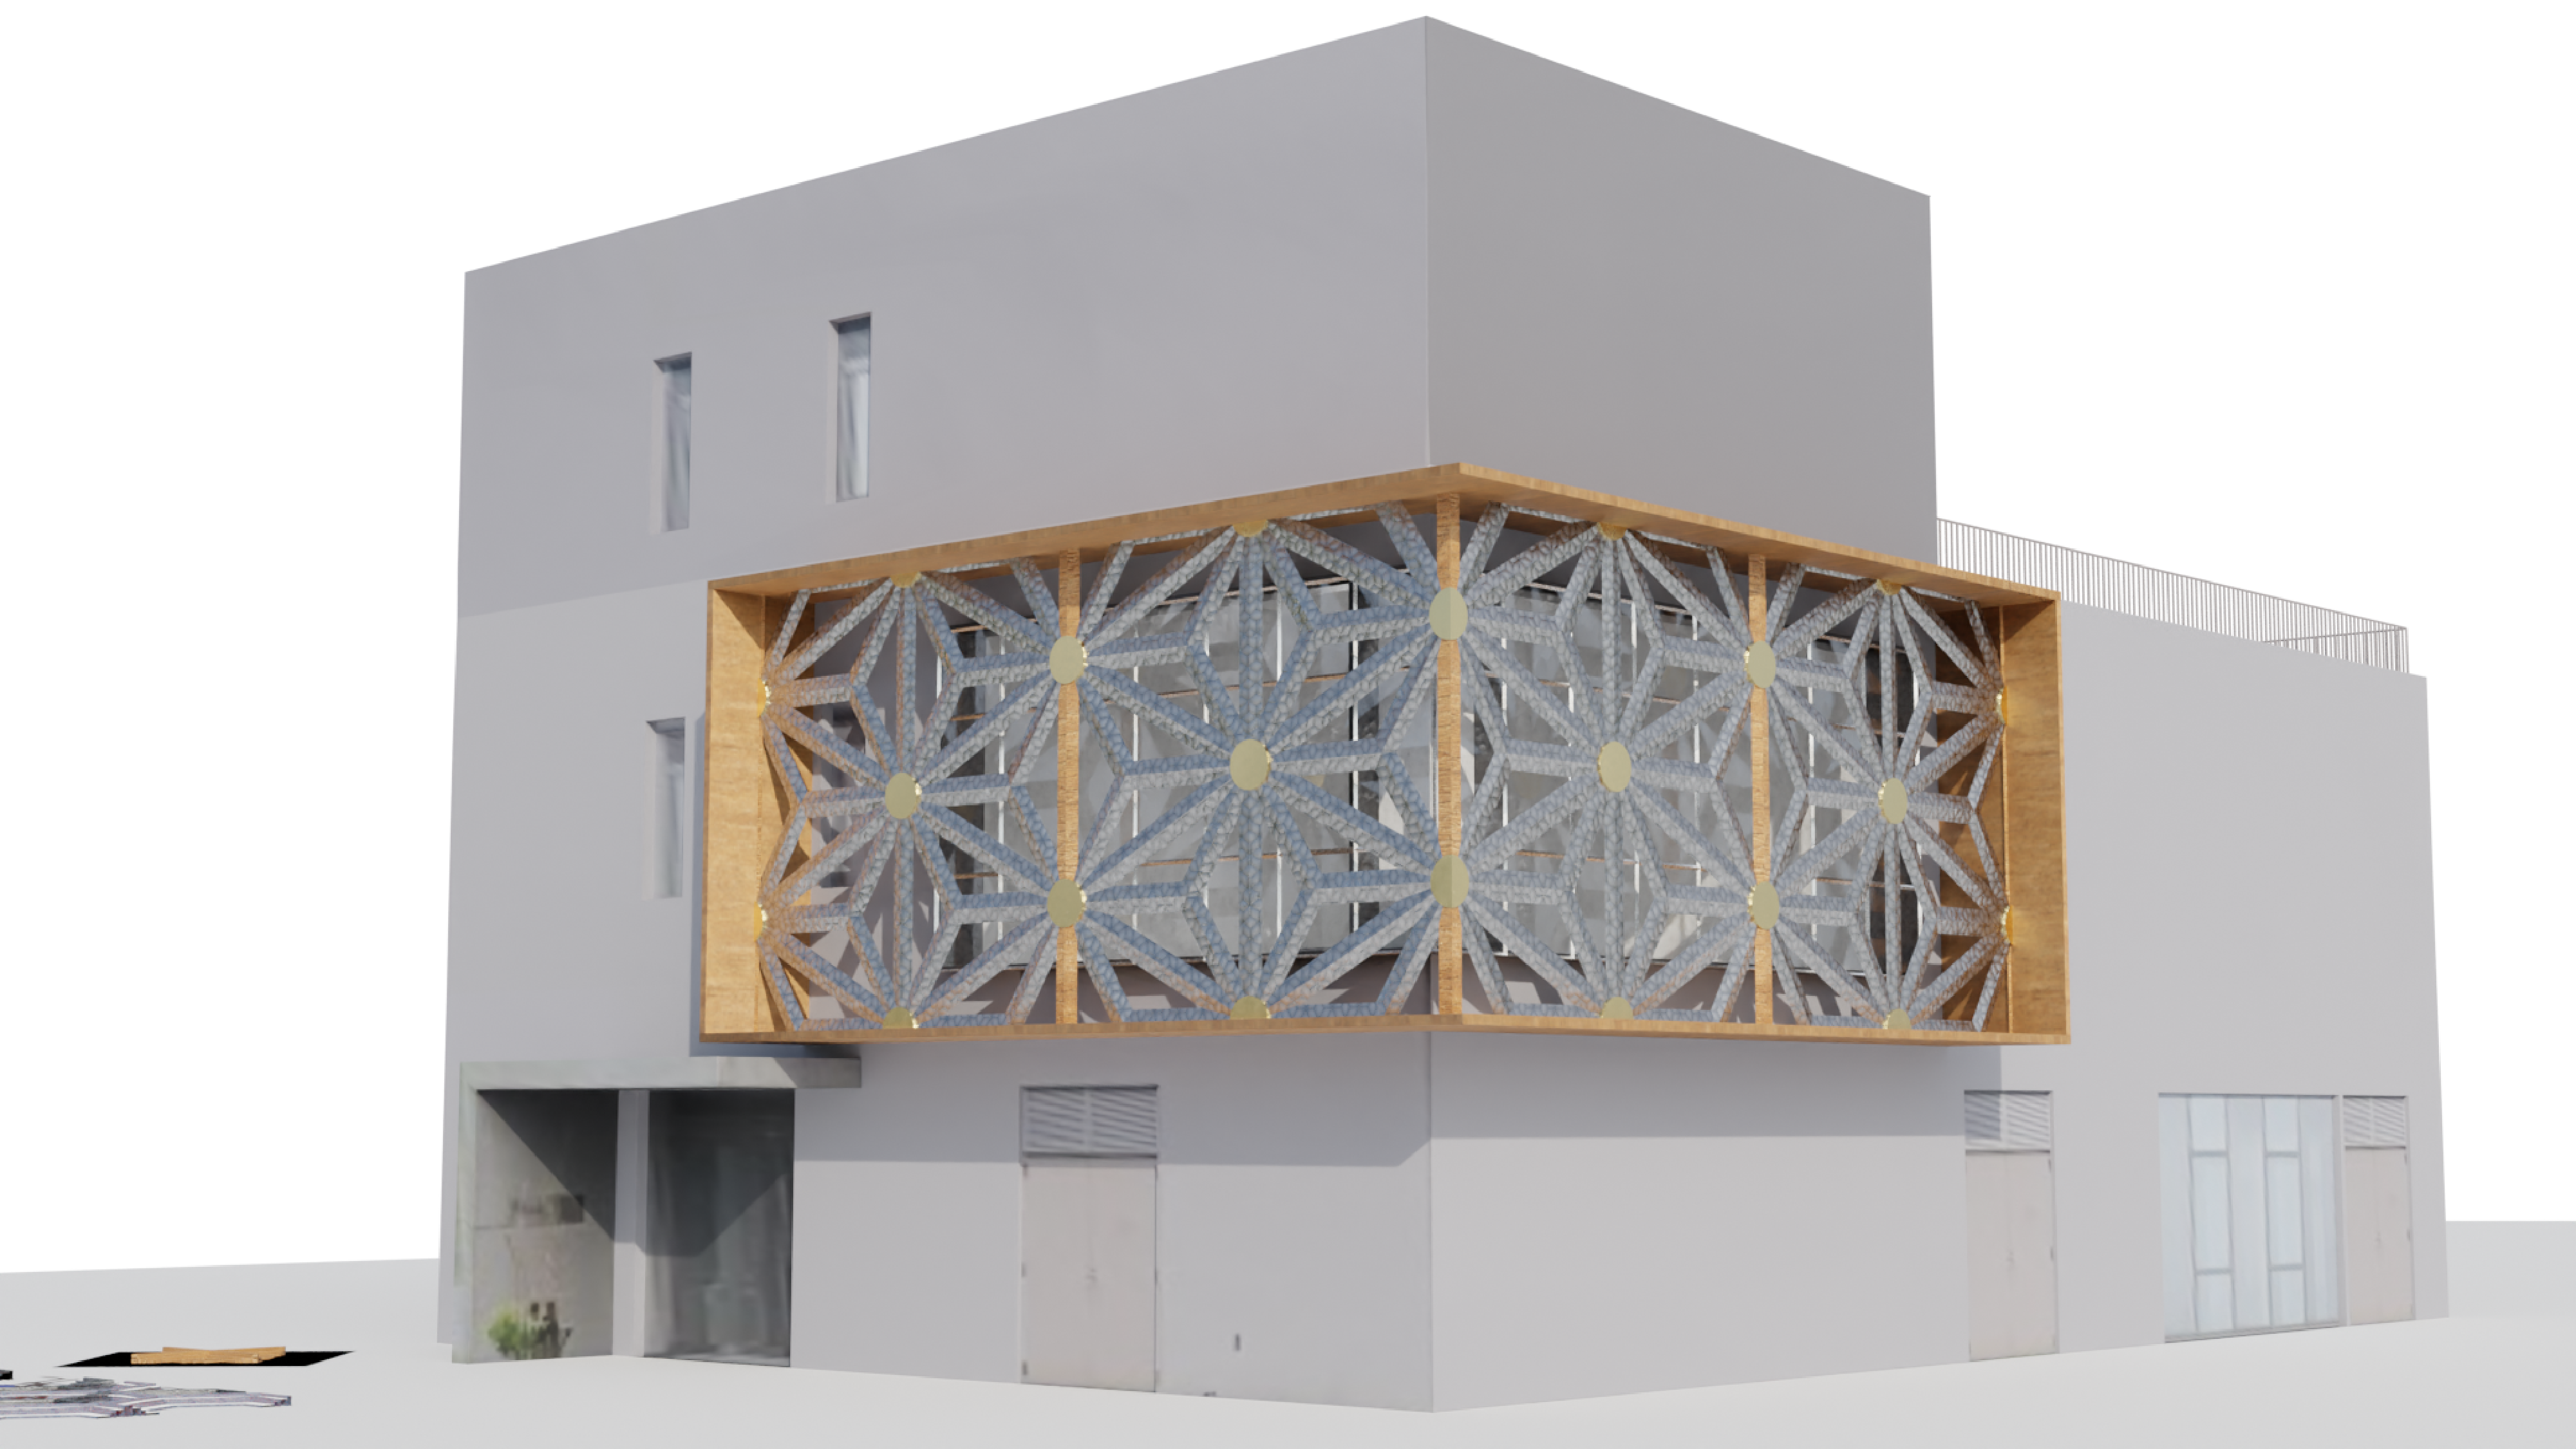
\includegraphics[width=1\linewidth]{Images/Pattern 3/0001}} \\
        \midrule
        \textit{Level 3} &  &  &
        \\
        {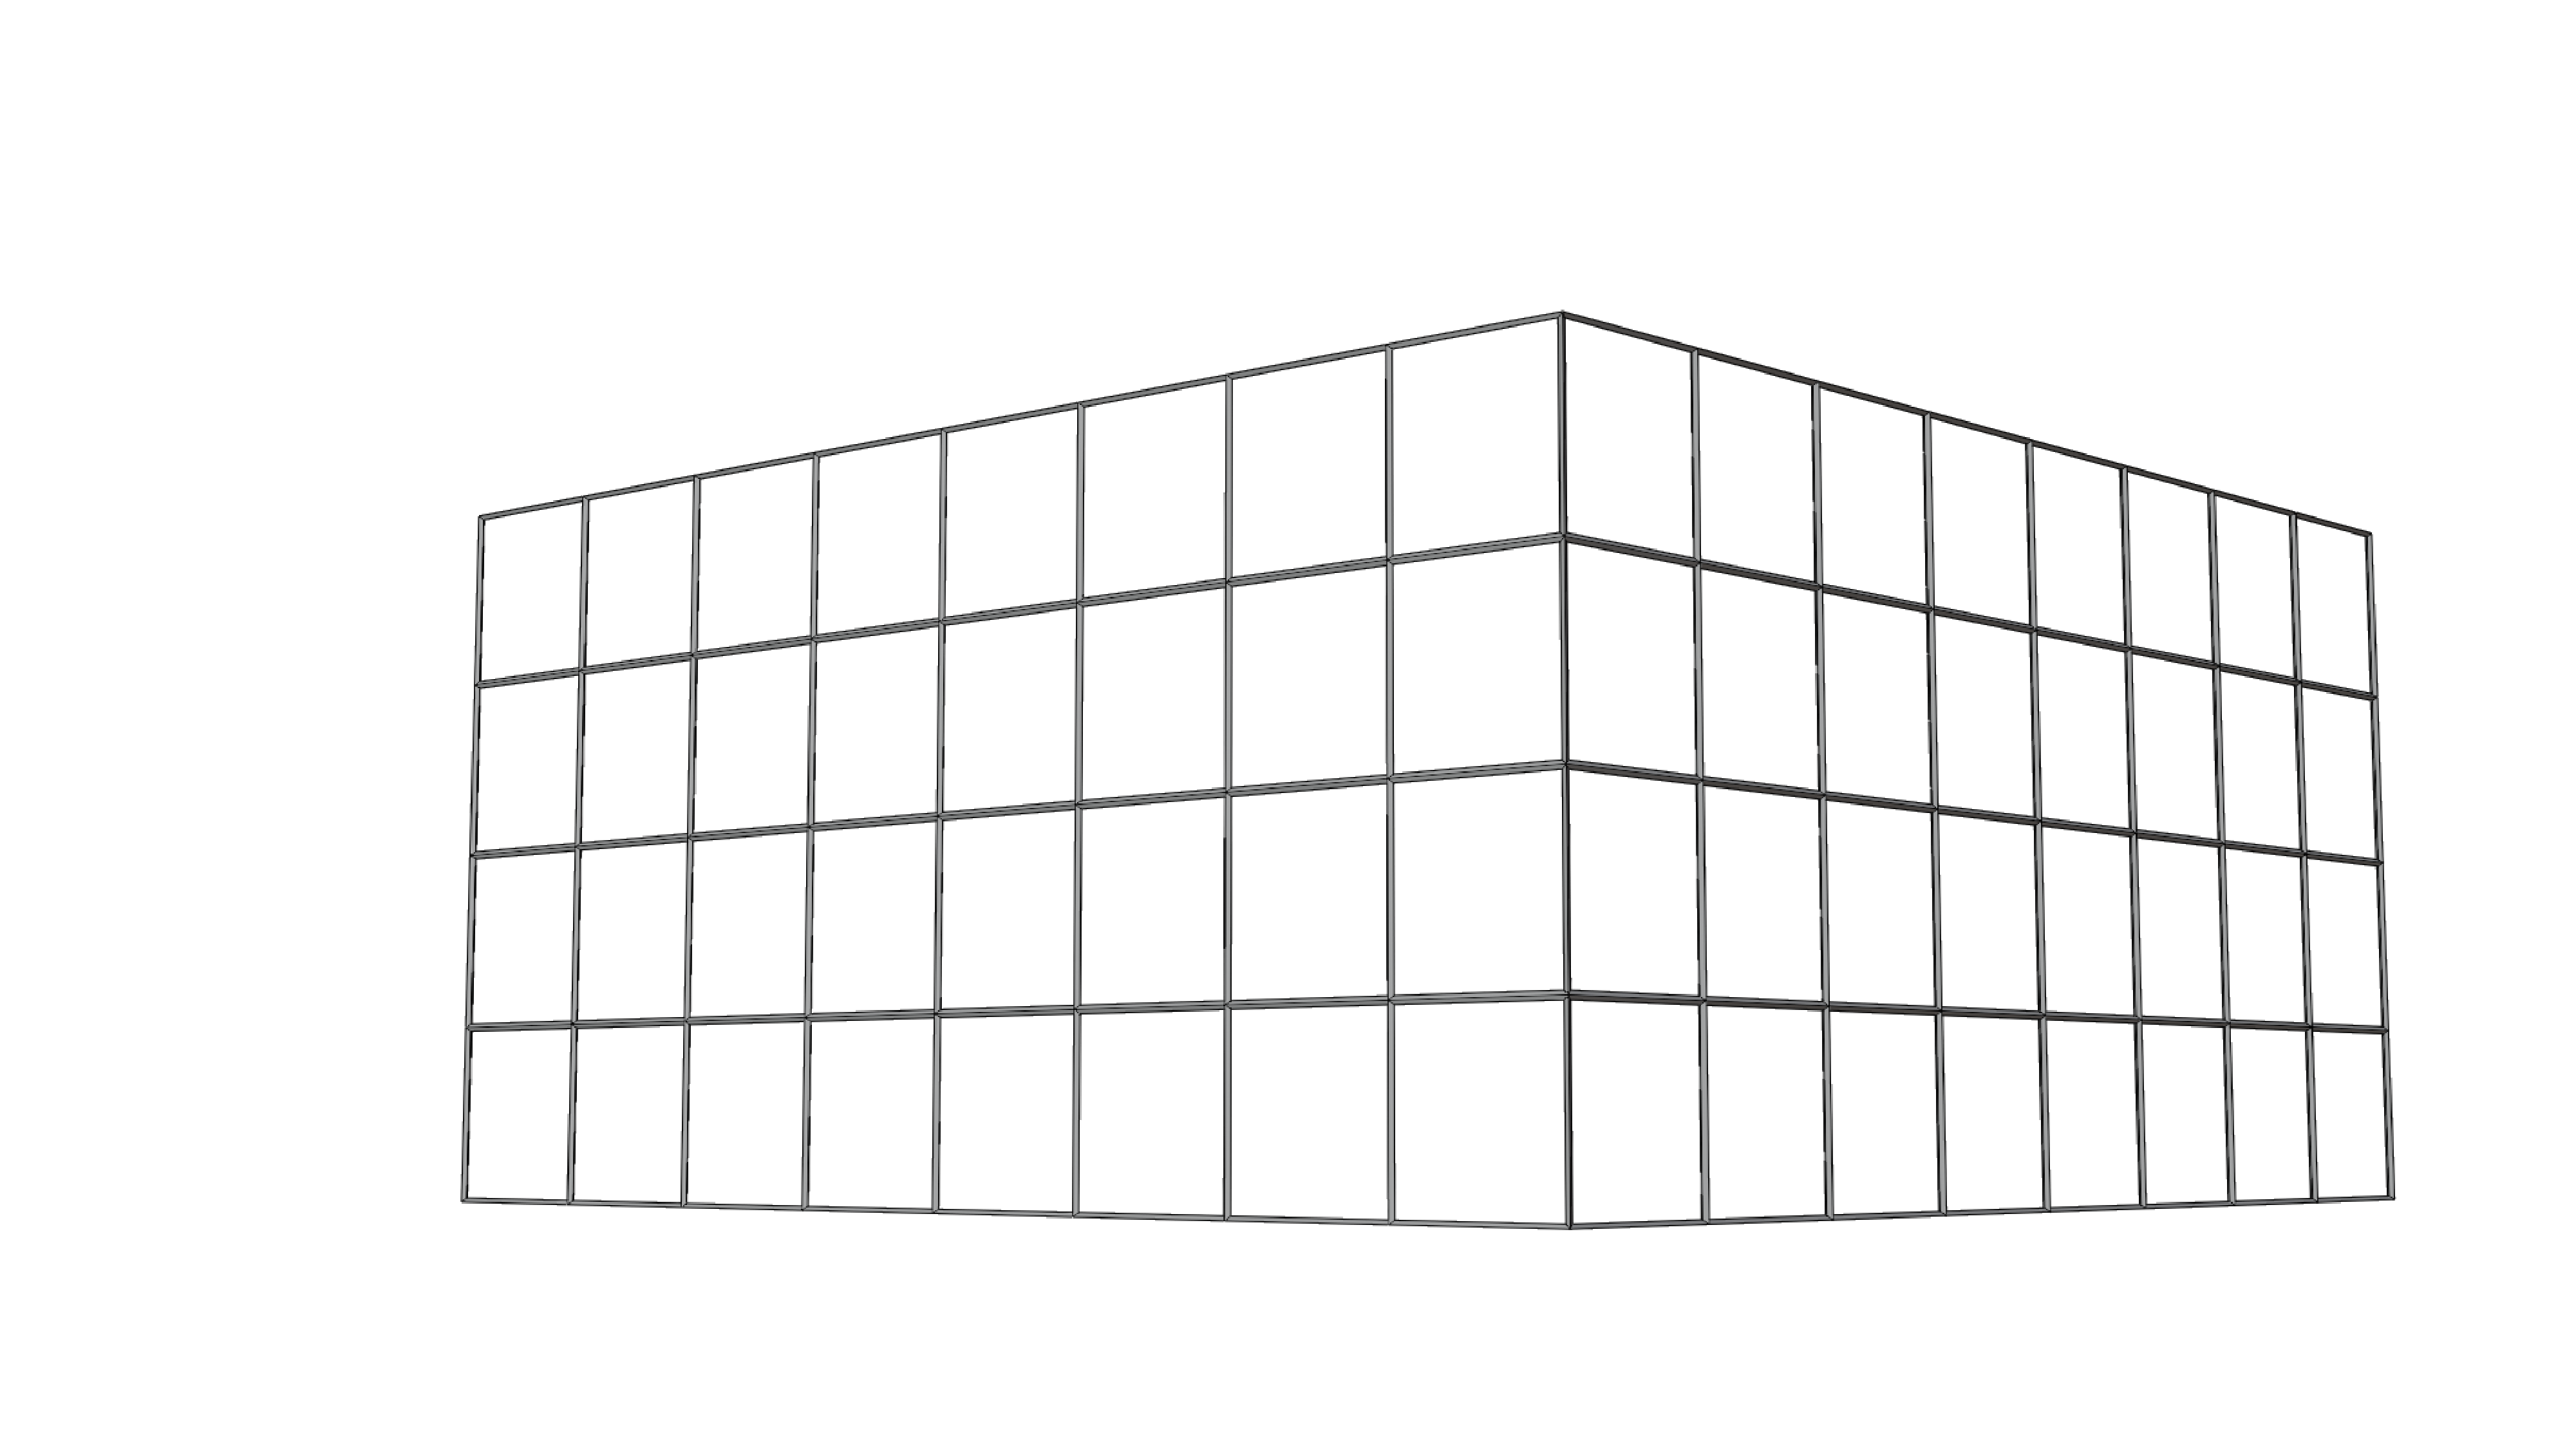
\includegraphics[width=1\linewidth]{Images/Wall 0/0003}} &
          {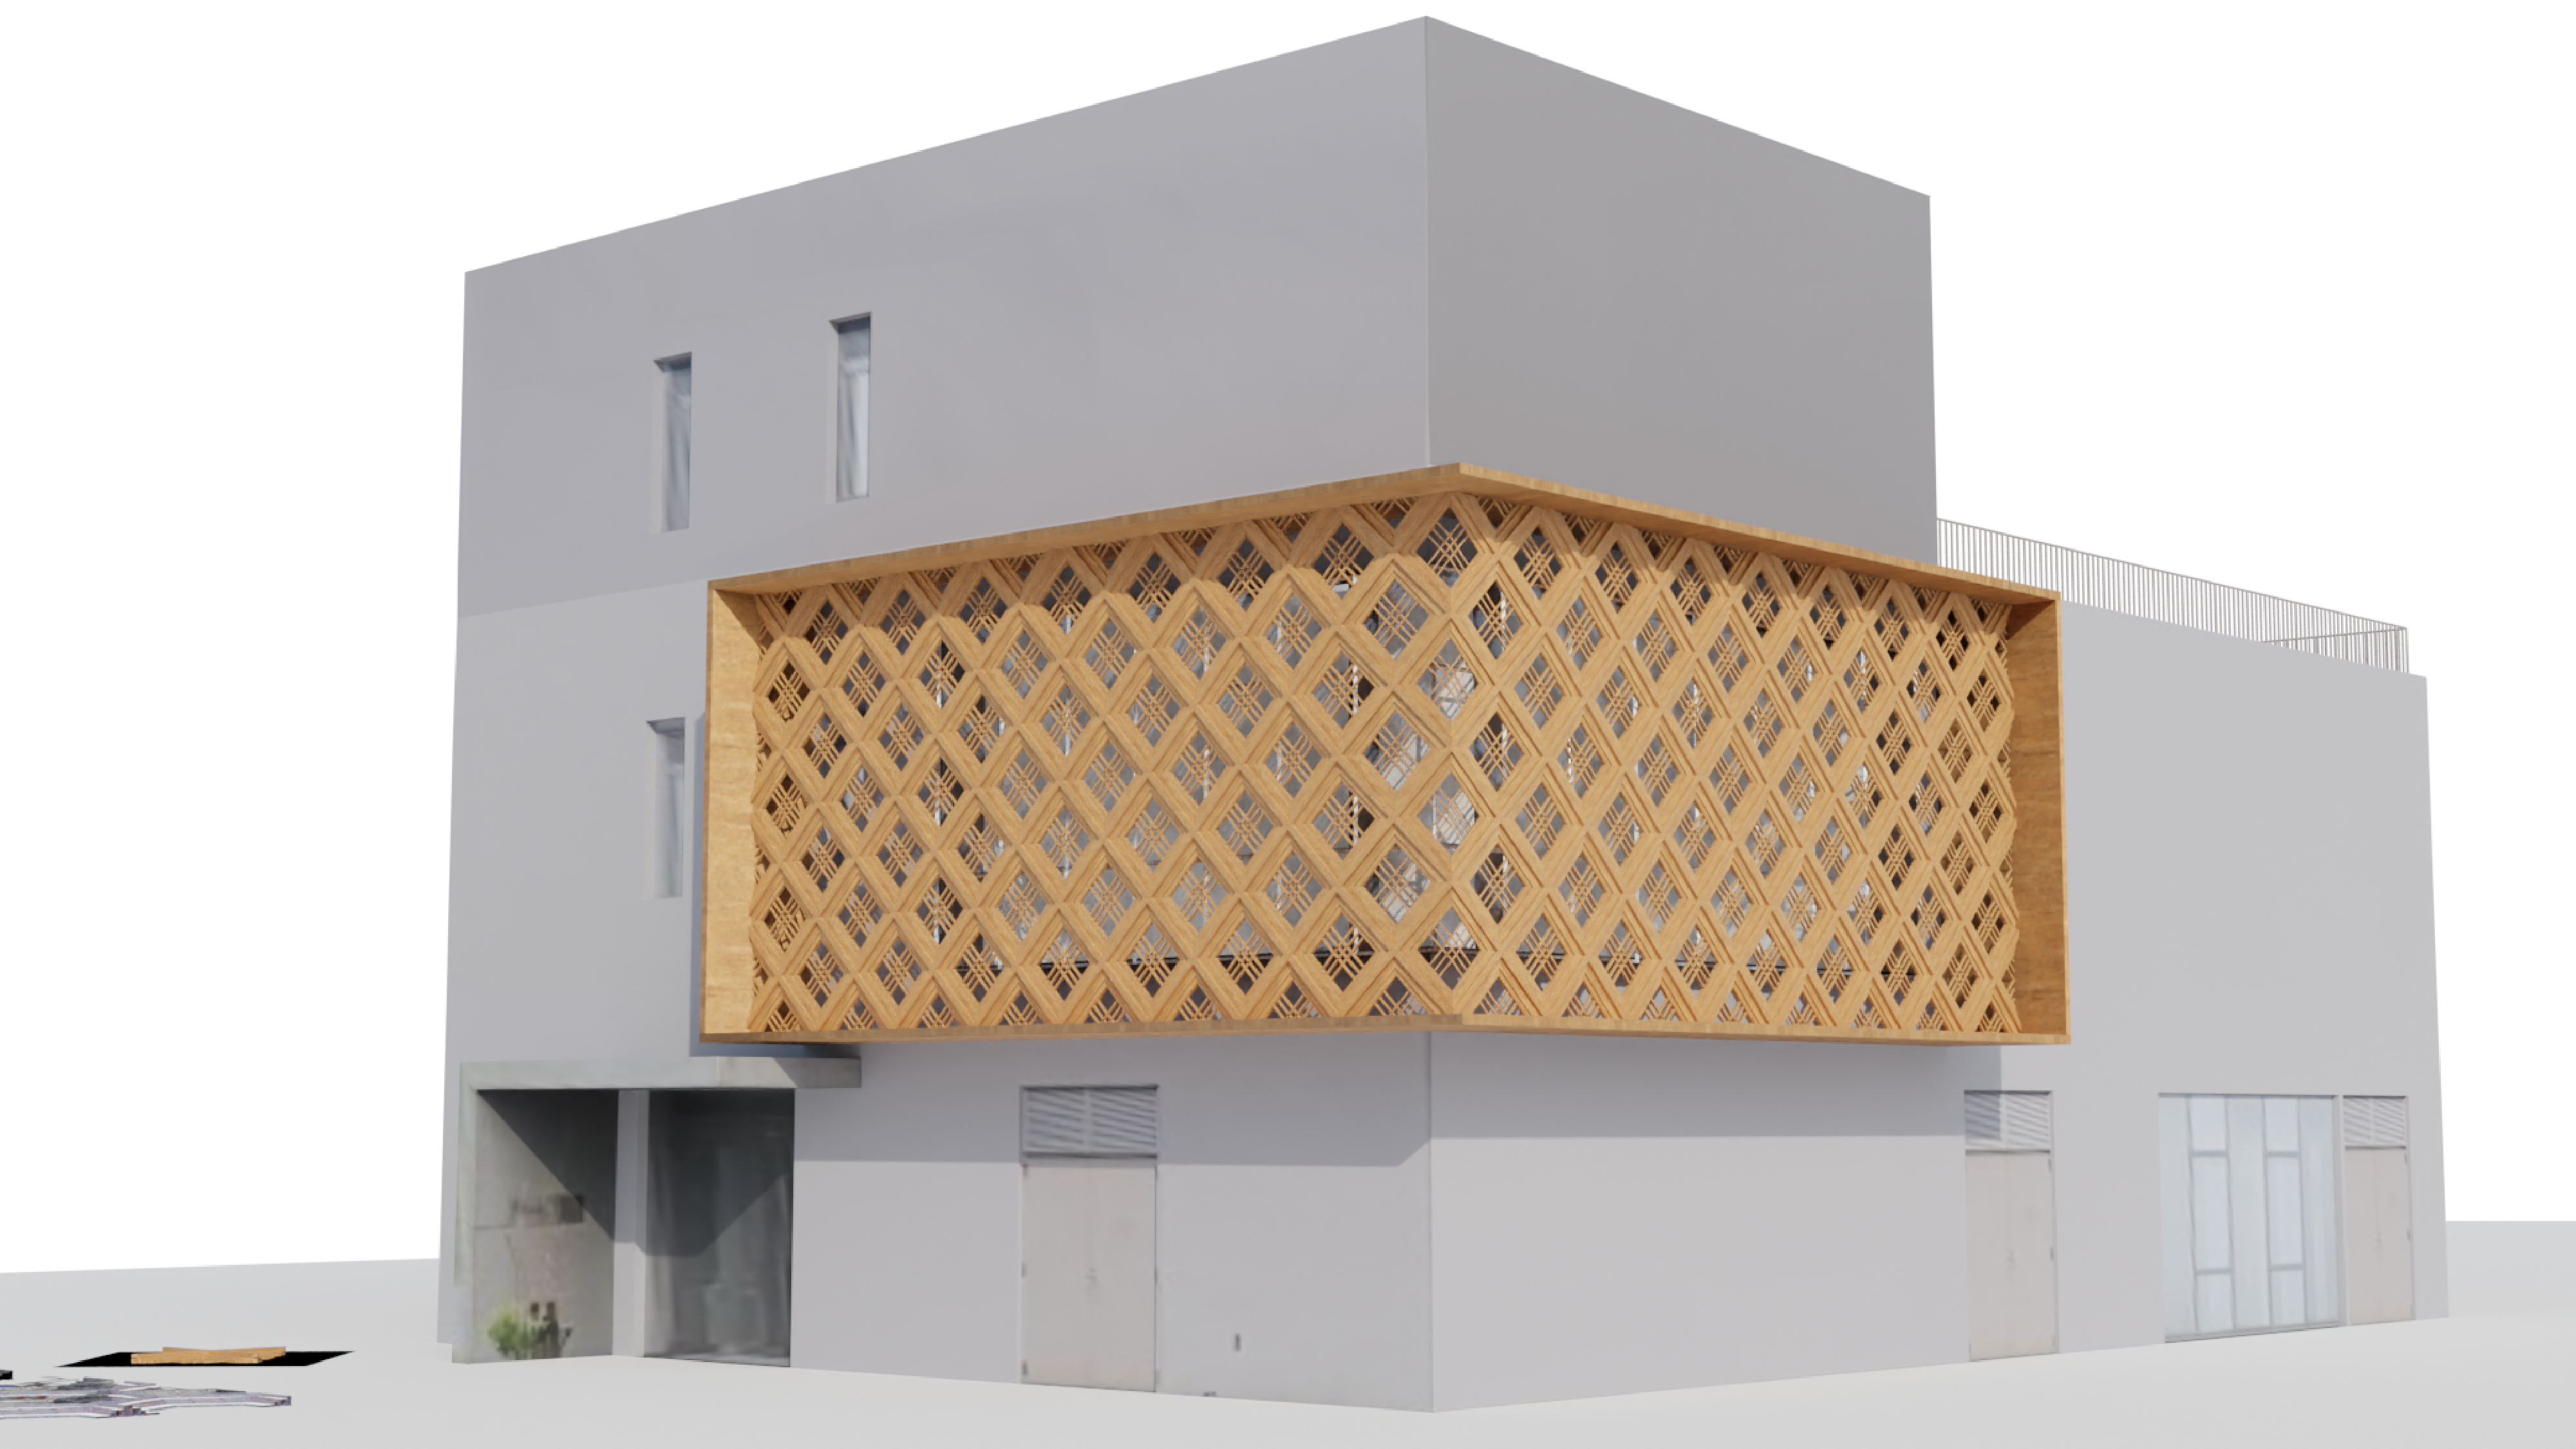
\includegraphics[width=1\linewidth]{Images/Pattern 1/0003}} &
          {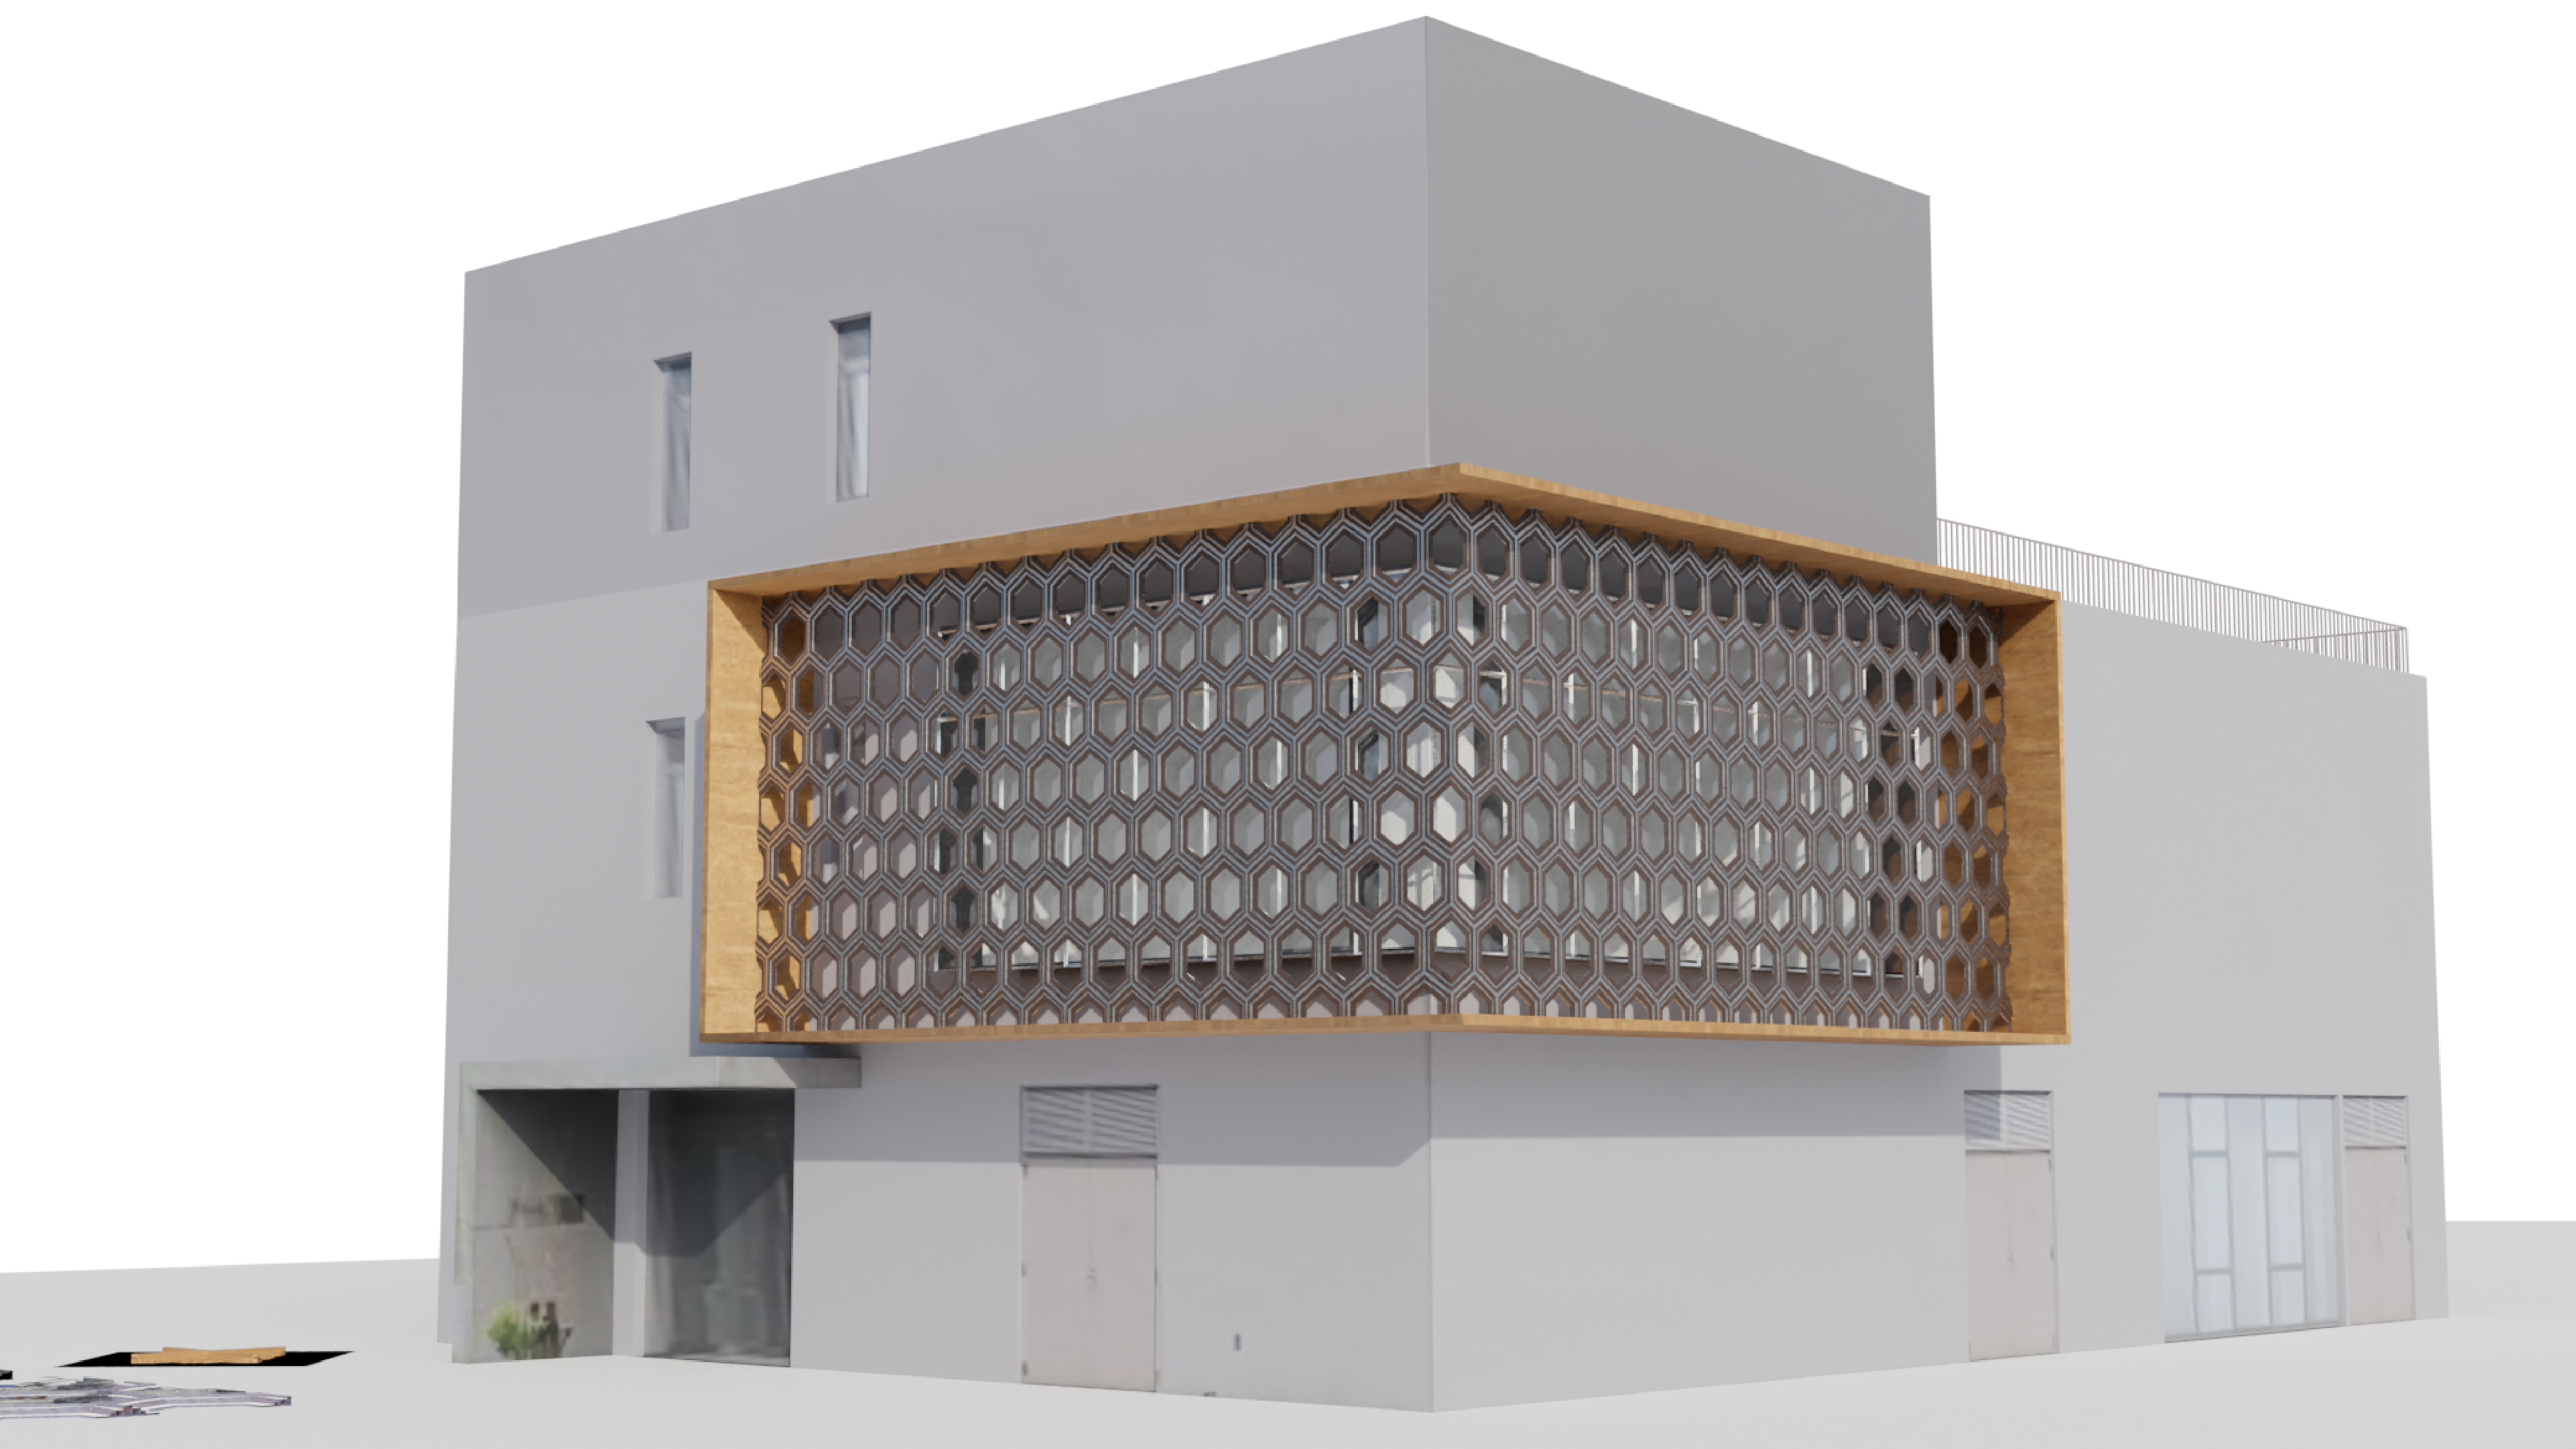
\includegraphics[width=1\linewidth]{Images/Pattern 2/0003}} &
          {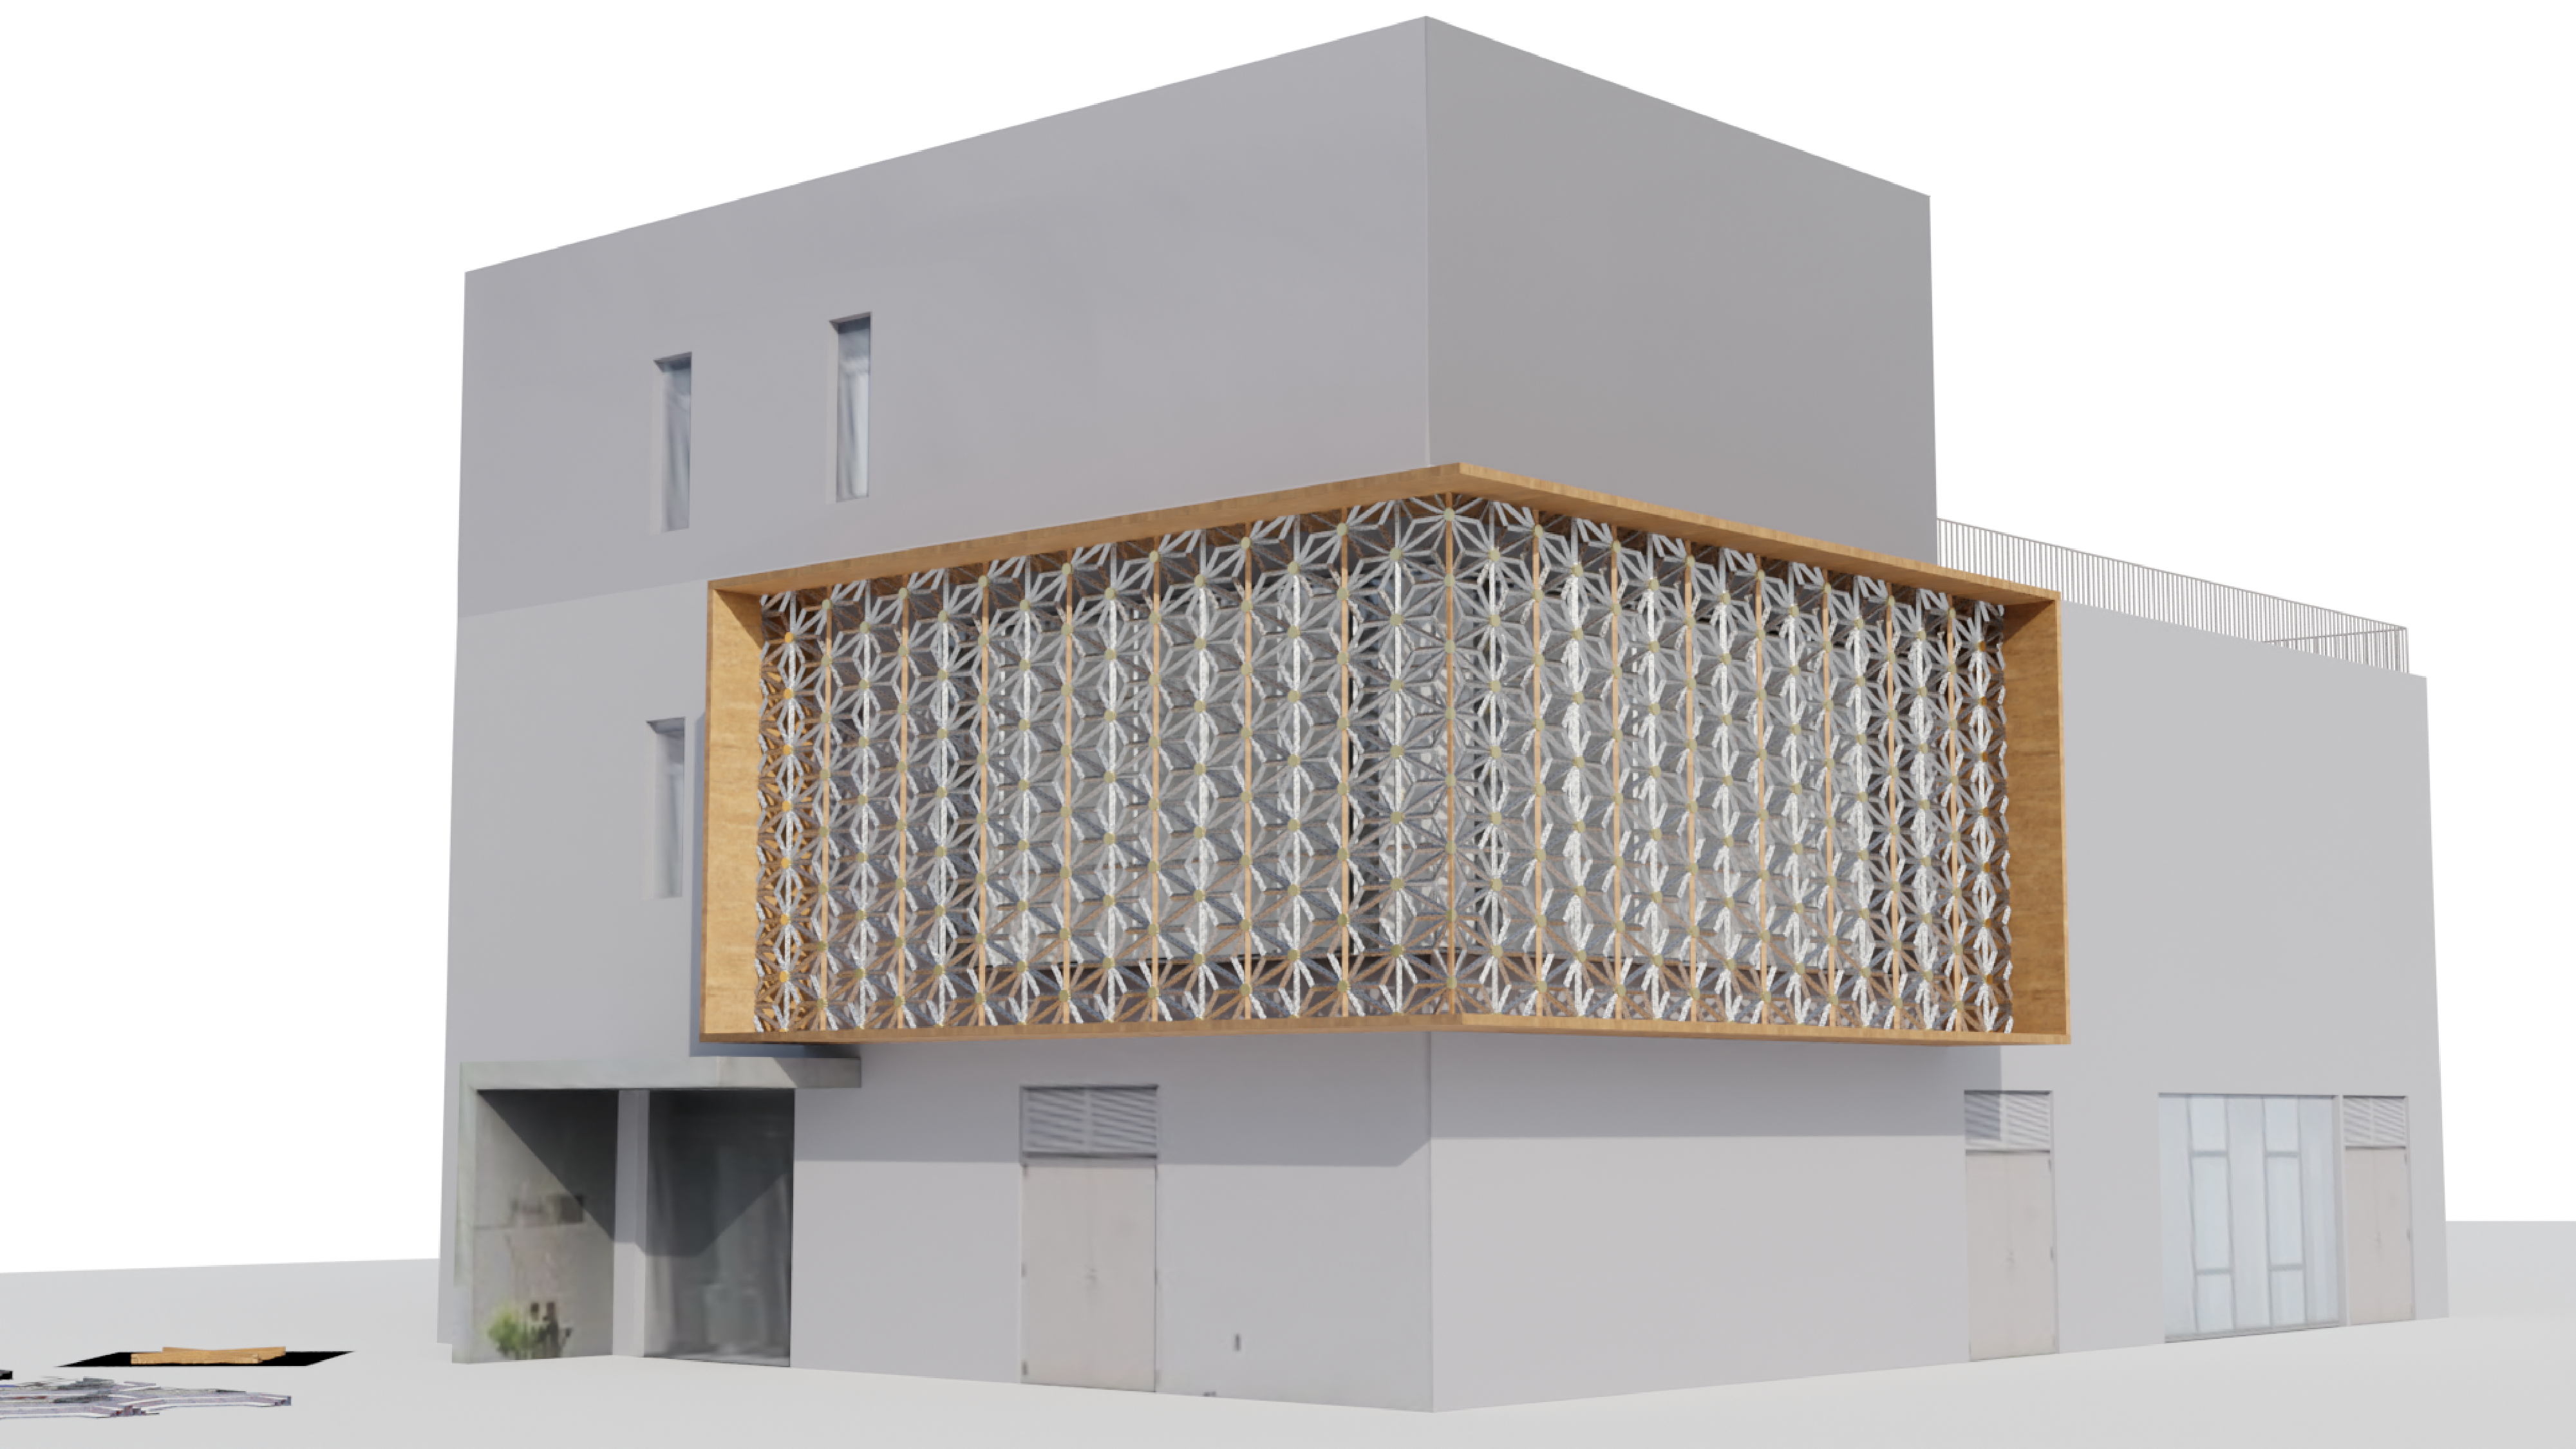
\includegraphics[width=1\linewidth]{Images/Pattern 3/0003}} \\
        \midrule
        \text{Level 9} &  &  &
        \\
        {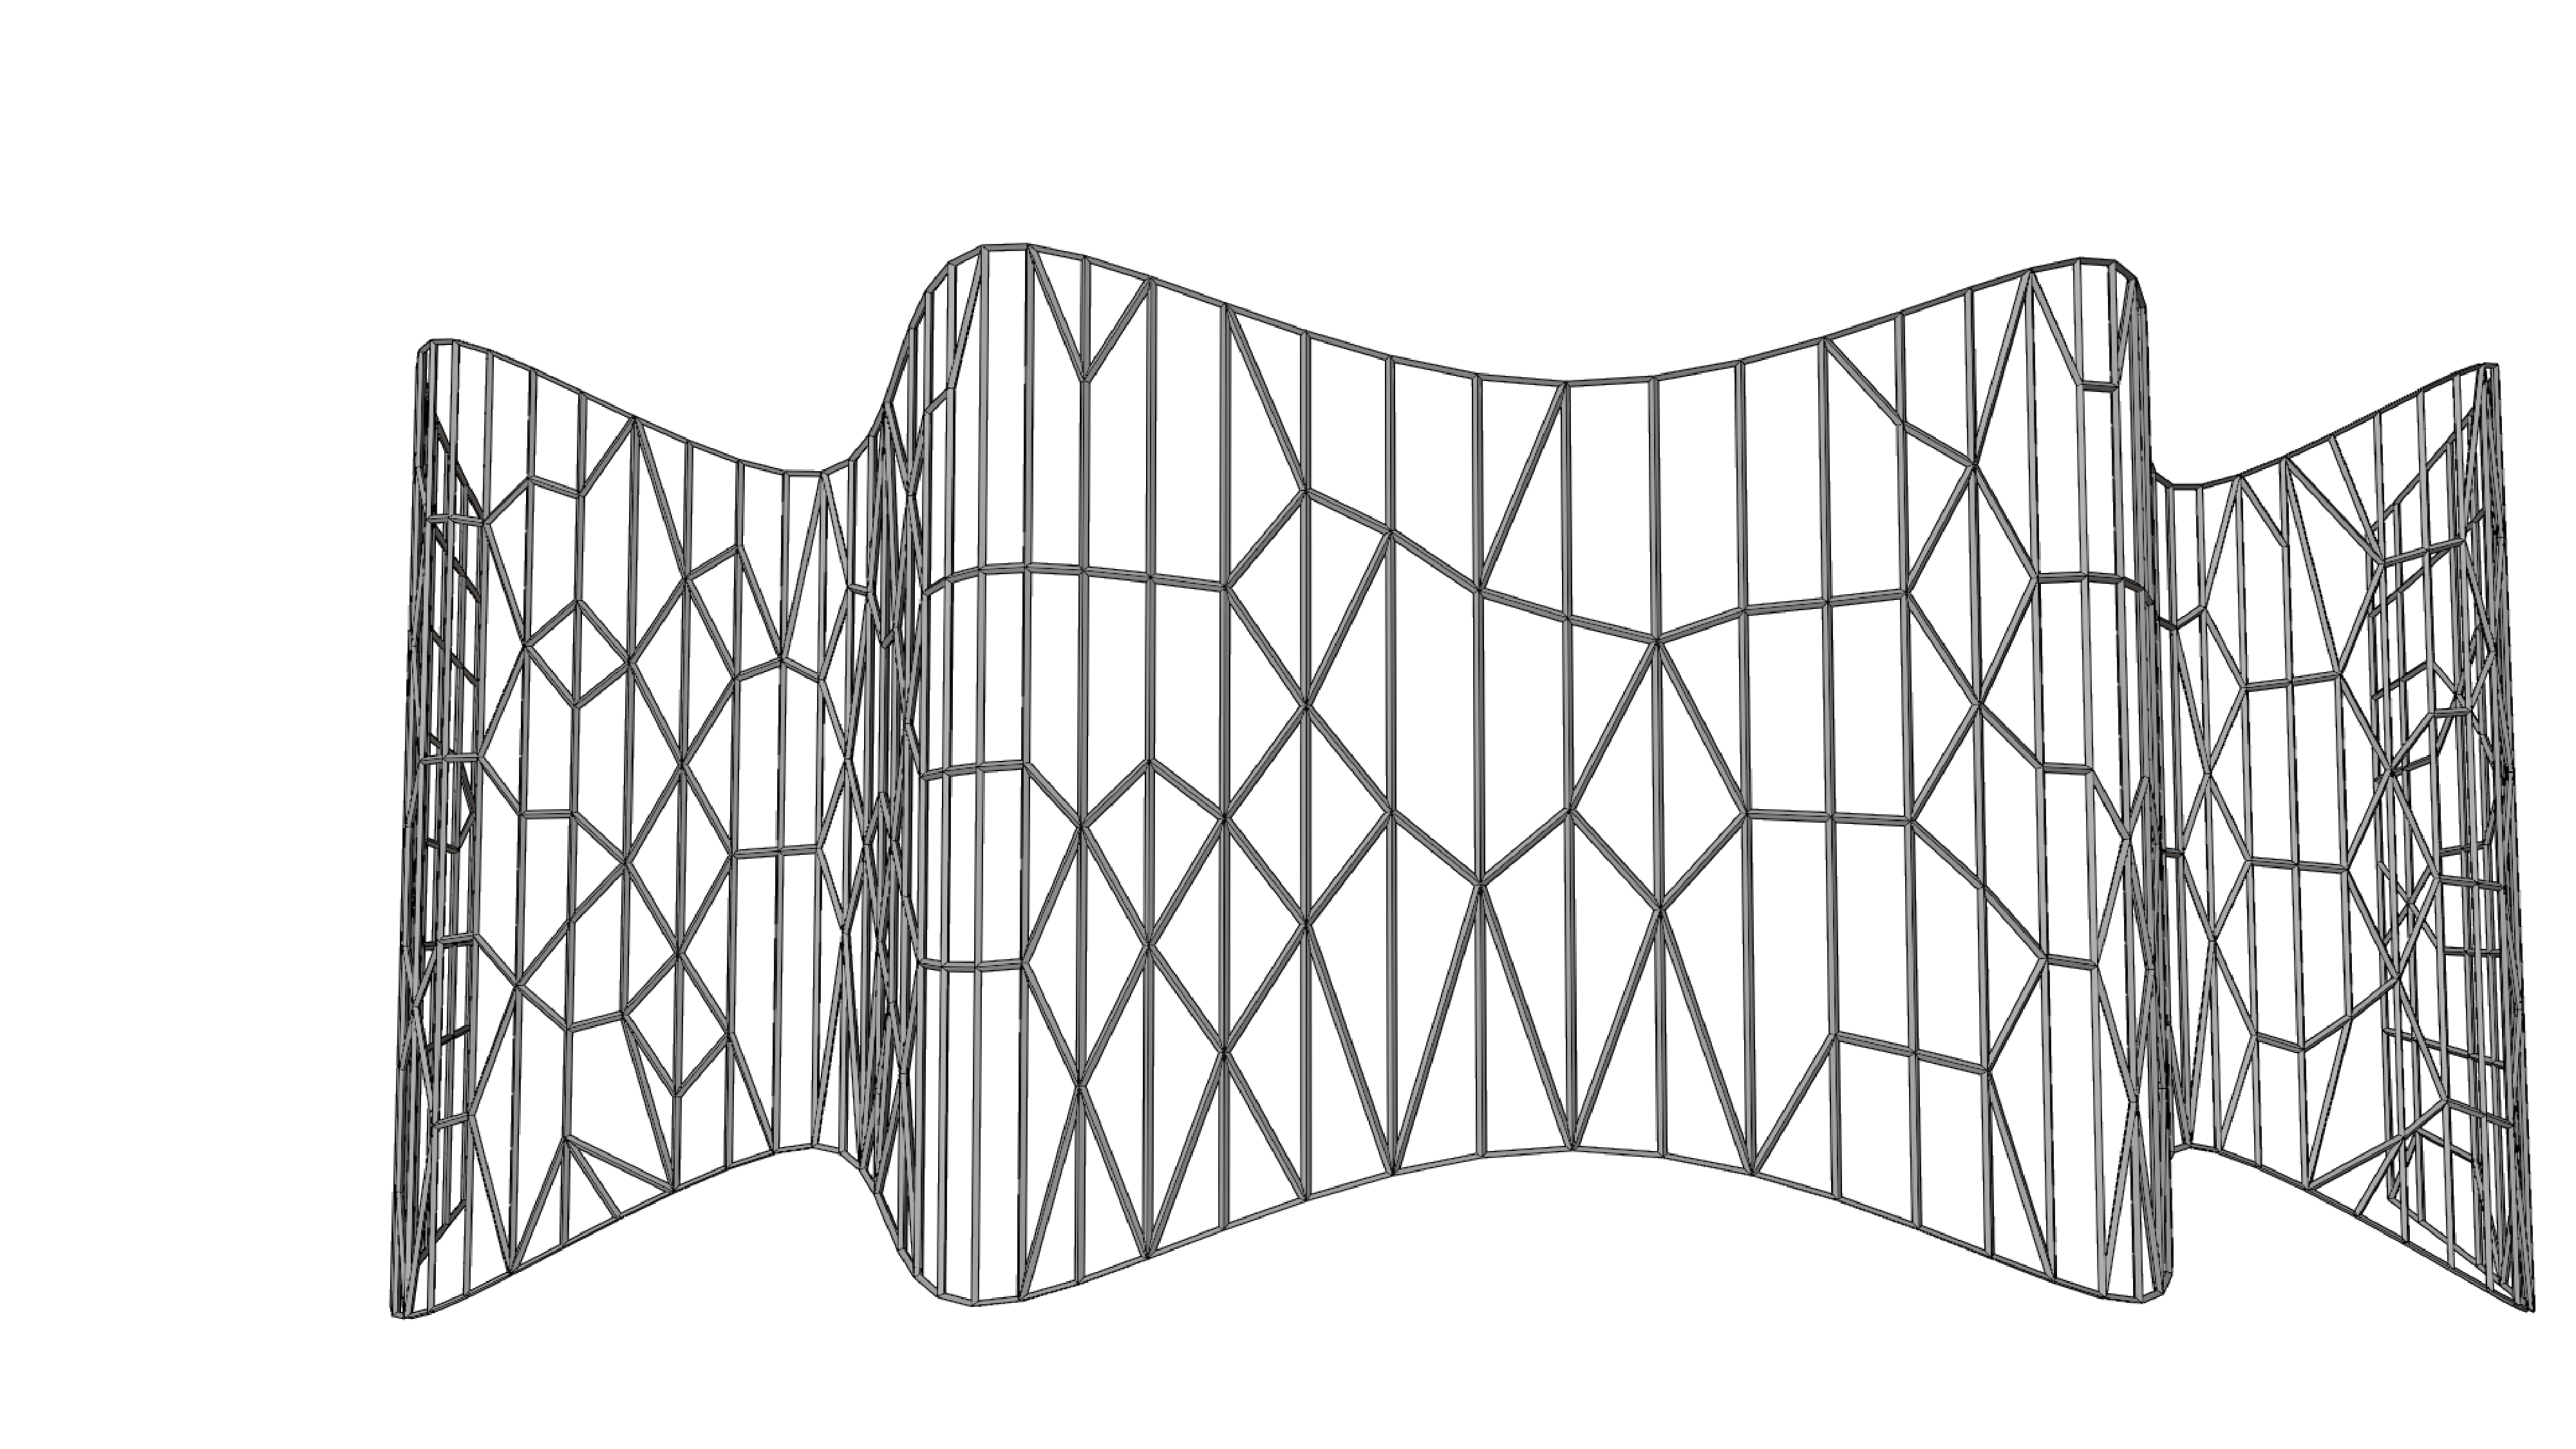
\includegraphics[width=1\linewidth]{Images/Wall 0/0009}} &
          {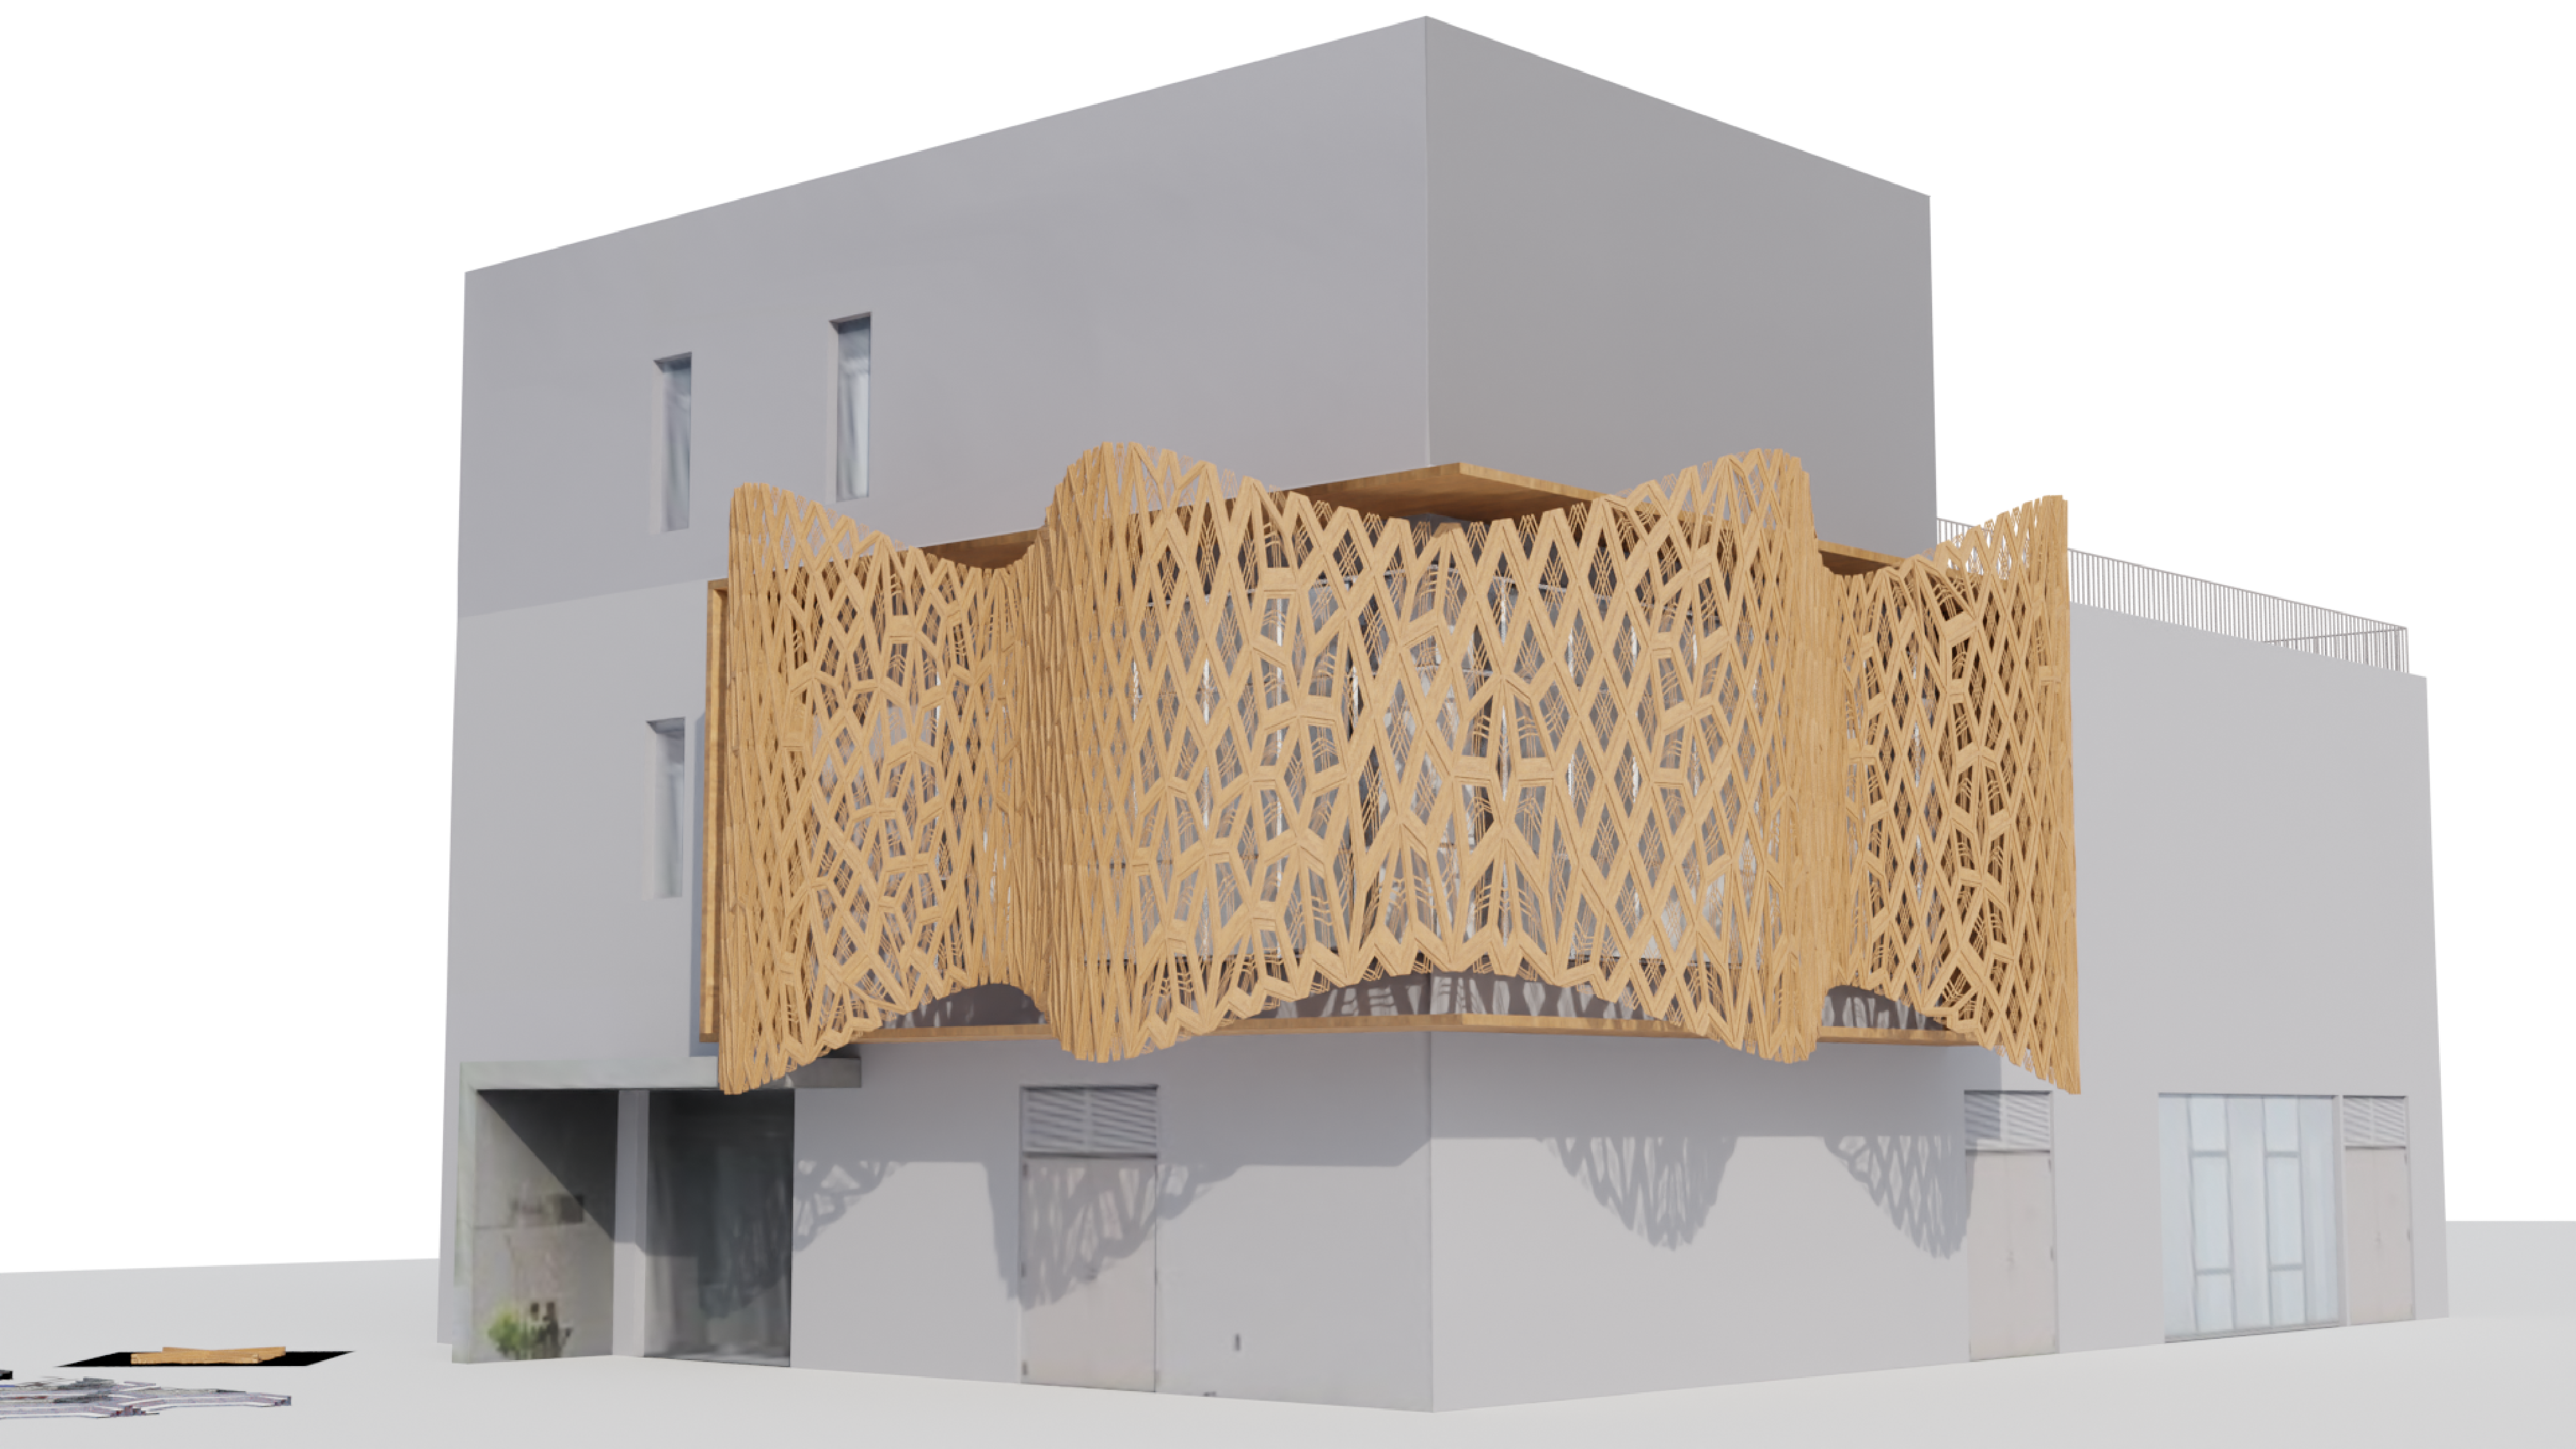
\includegraphics[width=1\linewidth]{Images/Pattern 1/0009}} &
          {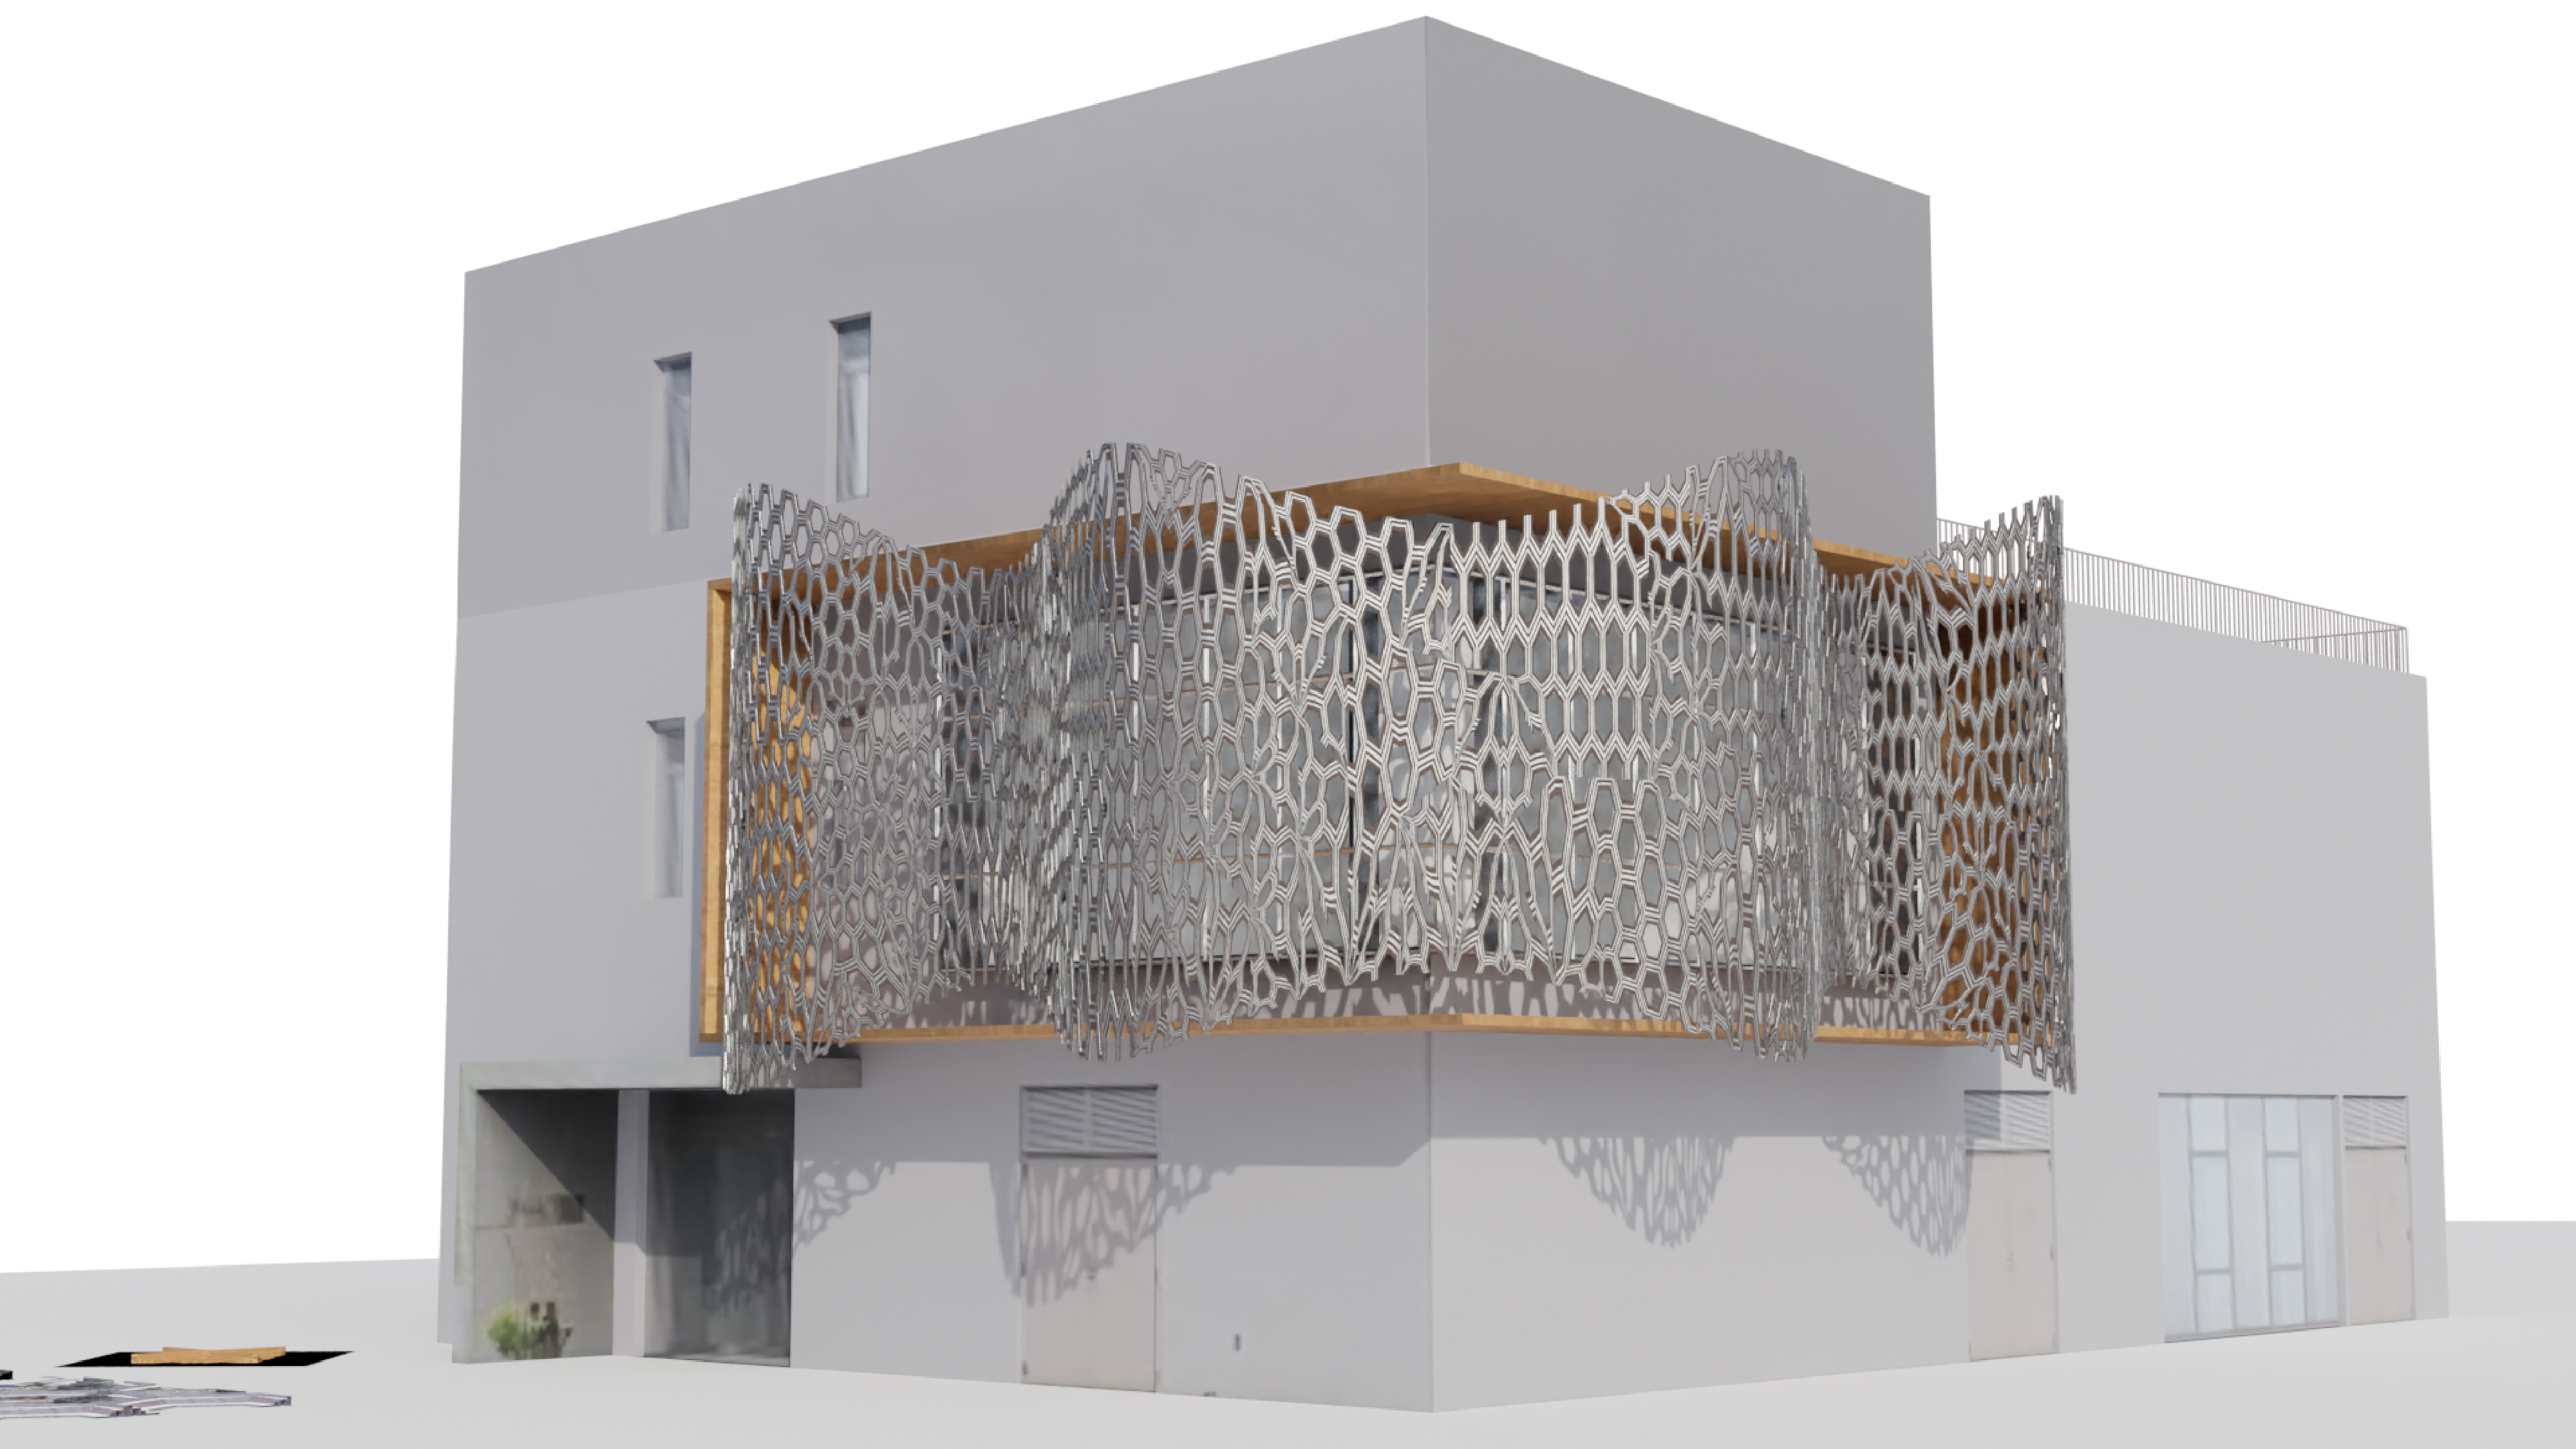
\includegraphics[width=1\linewidth]{Images/Pattern 2/0009}} &
          {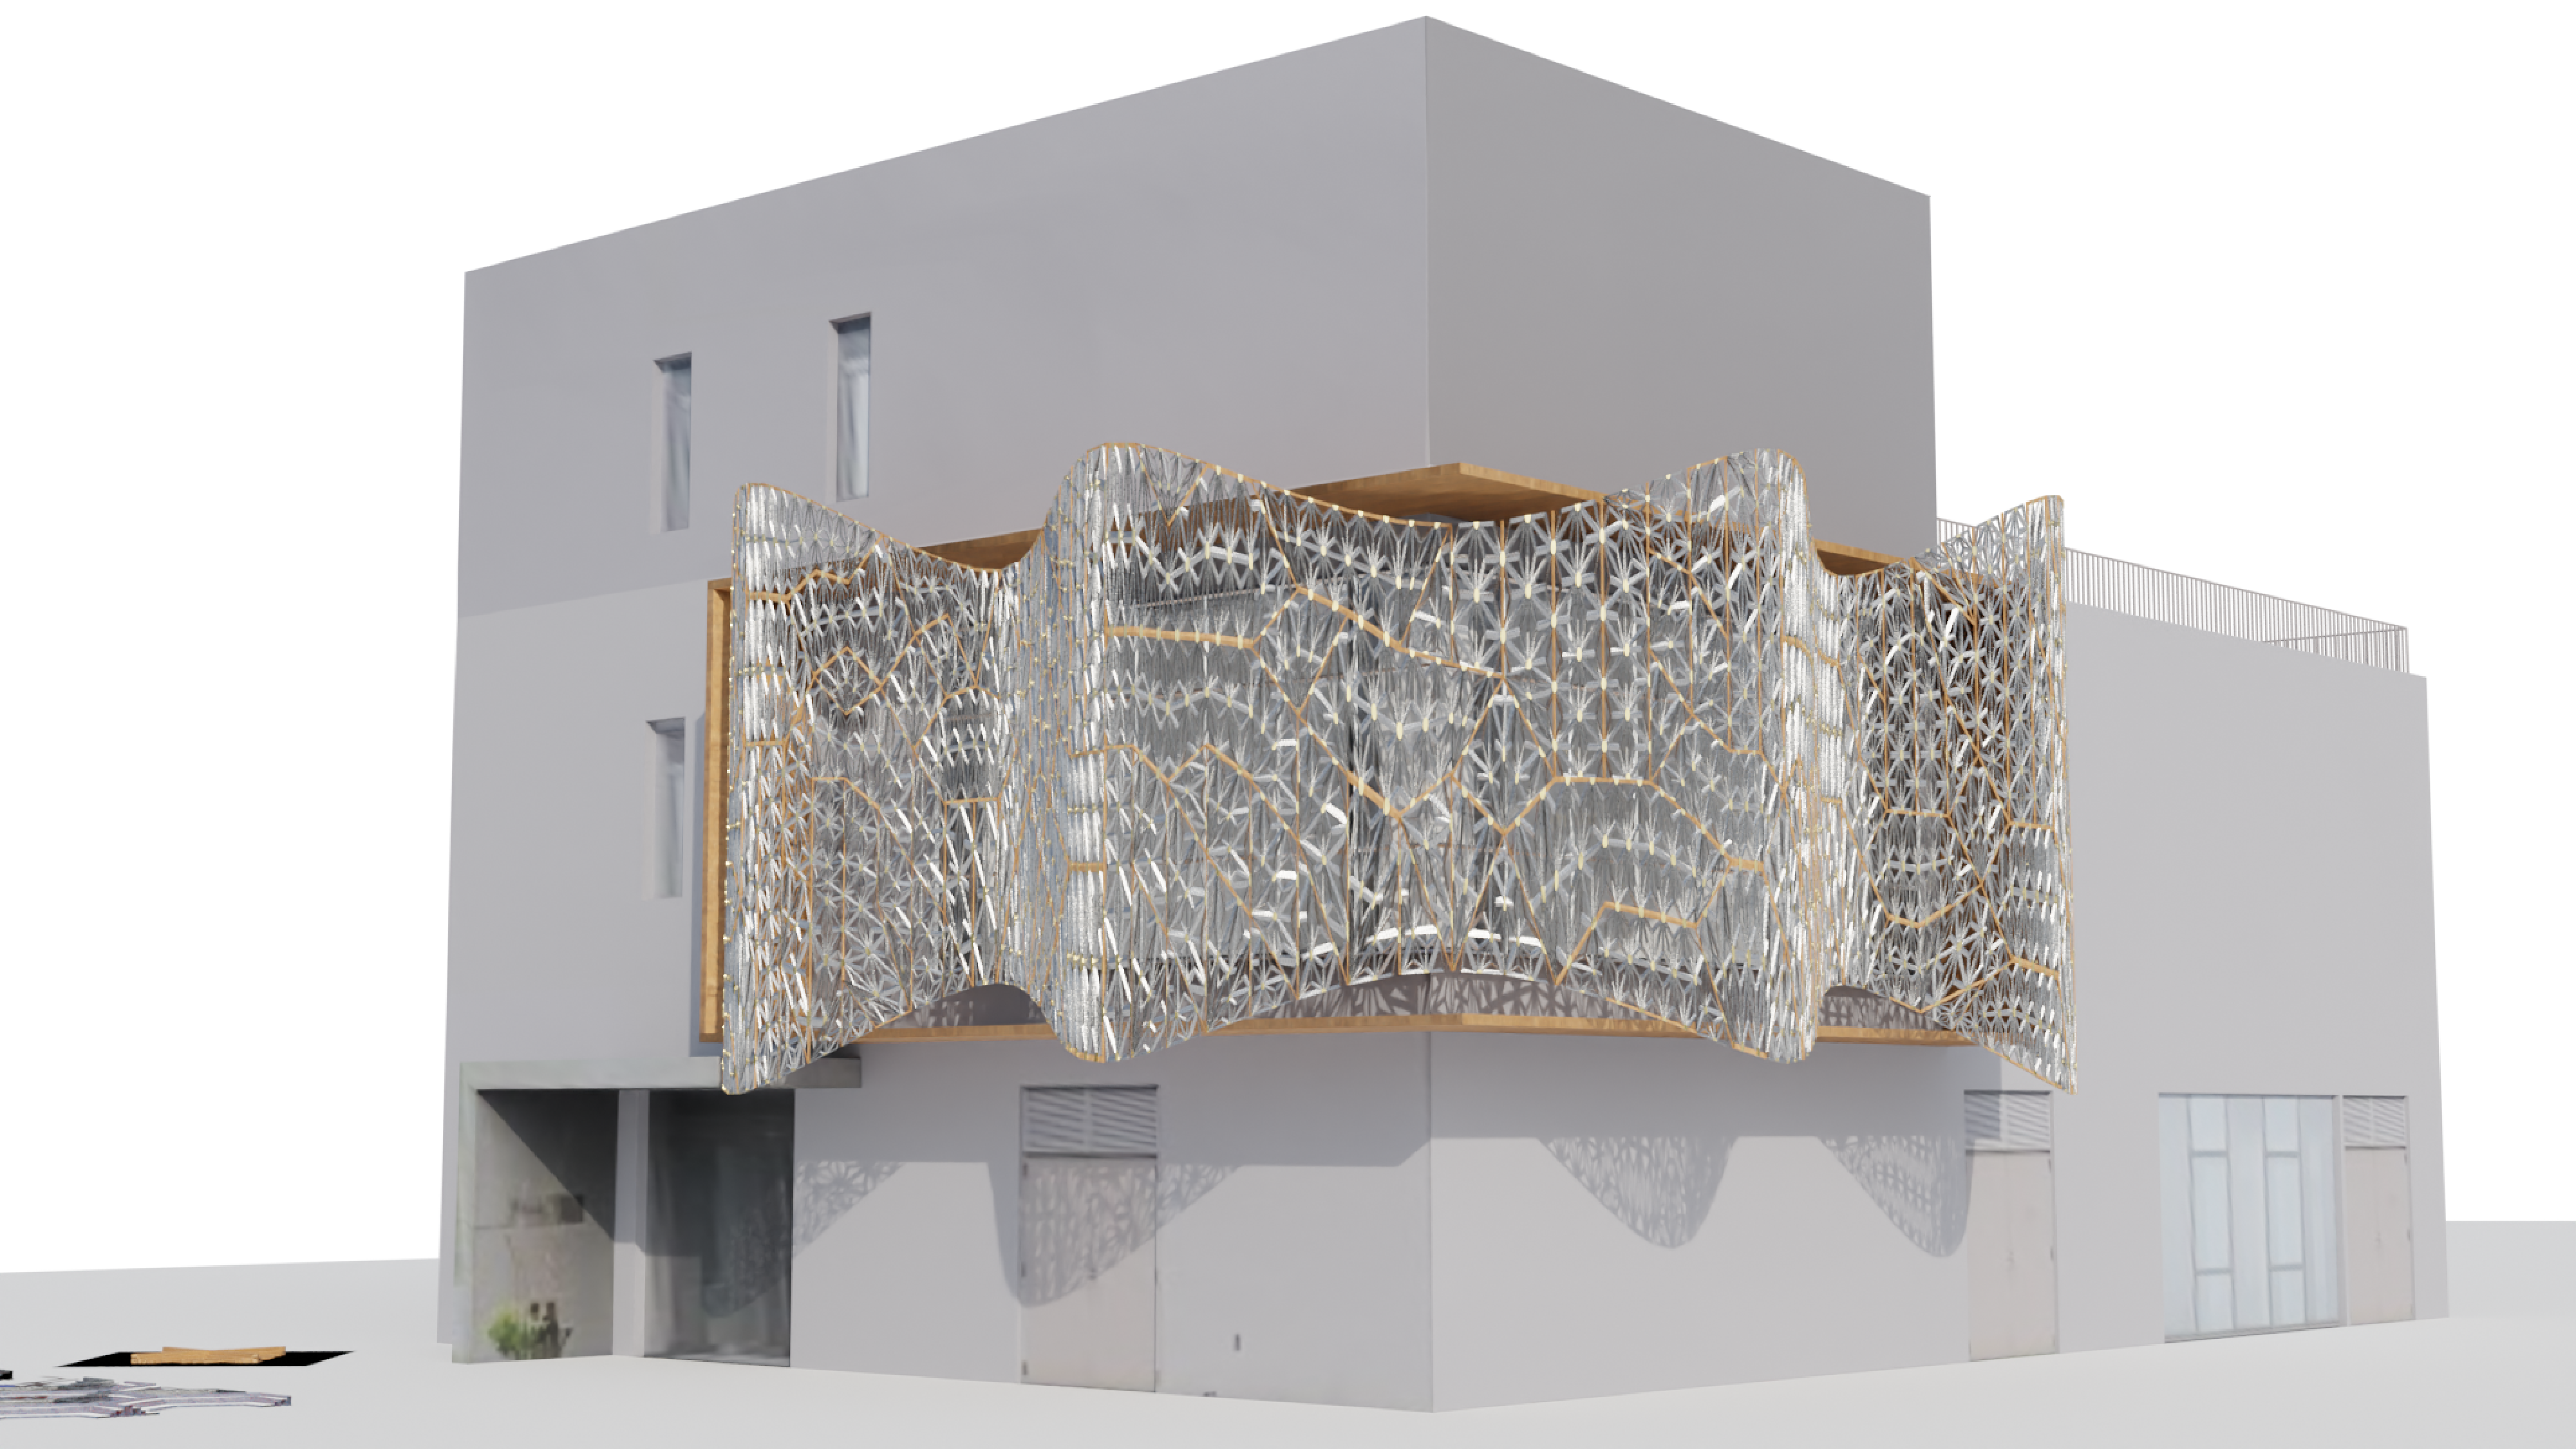
\includegraphics[width=1\linewidth]{Images/Pattern 3/0009}} \\
        \bottomrule
    \end{tabularx}
        \end{minipage}
    \end{tabular}
    \end{table*}



    \subsection{Complexity Analysis System Development}
    \label{subsec:ComplexitySystemDevelopment}
    %    \subsection{VR system for Complexity Analysis in facade design}
%    \label{subsec:VRsystemDevelopment}
%    %    \subsection{VR system for Complexity Analysis in facade design}
%    \label{subsec:VRsystemDevelopment}
%    \input{text/Method_1ComplexitySystemDevelopment.tex}VR System development
%! Concise

The `Complexity Analysis' system addresses the challenge of quantifying complexity in architectural facade design, playing a pivotal role in our study.
To achieve this, we developed a process that integrates immersive VR experiences with CV algorithms embedded in the CICA system (see Figure~\ref{fig:MethodologyFlowchartComplexity}, element 3.1).
This approach enables real-time interaction with various facade designs while providing complexity data, offering comprehensive insights into the aesthetic and practical implications of architectural complexity.

The system comprises three integral components: `\textit{3D Modeling and Environment Setup}', `\textit{CICA System}', and `\textit{VR Integration and Simulation Tools}'.
These components are illustrated in Figure~\ref{fig:MethodologyFlowchartComplexity} (labeled 1 to 3) and are detailed in the following sections.
VR System development
%! Concise

The `Complexity Analysis' system addresses the challenge of quantifying complexity in architectural facade design, playing a pivotal role in our study.
To achieve this, we developed a process that integrates immersive VR experiences with CV algorithms embedded in the CICA system (see Figure~\ref{fig:MethodologyFlowchartComplexity}, element 3.1).
This approach enables real-time interaction with various facade designs while providing complexity data, offering comprehensive insights into the aesthetic and practical implications of architectural complexity.

The system comprises three integral components: `\textit{3D Modeling and Environment Setup}', `\textit{CICA System}', and `\textit{VR Integration and Simulation Tools}'.
These components are illustrated in Figure~\ref{fig:MethodologyFlowchartComplexity} (labeled 1 to 3) and are detailed in the following sections.


%!% CICA tables and function
    %Table PI table, Function1, CICA evaluation process on architectural facades. Table 1x3
    \begin{table*}[htb]
    \centering
    \small
    \begin{tabular}{c}
        %Top cell with one figure
        %Table: Performance Indicators
        \begin{minipage}{\textwidth}
            \centering
            \captionof{table}{Table of Metrics and Weights for Complexity Scoring: Outlines the key criteria and corresponding weights utilized in the CICA system to determine the `Complexity Score' of architectural facades, detailing the systematic approach to quantifying facade intricacy through edge density and contour count metrics.}
            \label{tab:MetricsandWeights}
            \begin{tabularx}{\textwidth}{p{2.5cm} p{1cm} X X p{1cm}}
                \toprule
                \multicolumn{5}{c}{\textbf{Table of Metrics and Weights for CICA Complexity Scoring on Architectural Facades}} \\
                \toprule
                \textit{Complexity metric} &
                  \textit{N} &
                  \textit{Metric name/description} &
                  \textit{Quantitative   method} &
                  \textit{Weights} \\ \midrule
                \textbf{Edge Density} &
                  1 &
                  Edge detection using Canny Edge Detection algorithm for highlighting the most relevant features of a building.
                    &
                  Measured by dividing the number of non-zero (edge) pixels in the edges image by the total number of pixels in the image.
                    &
                  8\\
                \\
                \textbf{Contour count} &
                  2 &
                  Employs contour approximation algorithm for shape analysis to determine intricacy of edges.
                    &
                  Measure by counting the number of segments in an edge.
                    &
                  2\\ \bottomrule
                   &
                   &
                  \textbf{TOTAL} &
                  &
                  \textbf{10}\\ \bottomrule
            \end{tabularx}
        \end{minipage}
        \\
        \\
        \\
        %Bottom cell
        %Table: CICA Image evaluation process for historical and 3d facades
        \begin{minipage}{\textwidth}
            \centering
            \captionof{table}{CICA Evaluation on Architectural Facades: The table presents a comparative analysis of CICA evaluation applied to 3D-modeled facades (a) and historical buildings (b). The process includes steps from original imagery to image processing (noise reduction, grayscale), edge detection, and contour count analysis, as shown on the flowchart in Figure\ref{fig:MethodologyFlowchartComplexity} (element 2). It highlights  the adaptability of CICA to assess complexity in both historical and contemporary architectural designs.}
            \label{tab:CICAImageEvalProcessOnArchitecturalFacades}
            \begin{tabularx}
            {\textwidth}{X X X X }
                \toprule
                \multicolumn{4}{c}{\textbf{CICA Image Evaluation process on Architectural Facades}} \\
                \toprule
                \multicolumn{1}{c}{\textit{Original Image}} &
                 \multicolumn{1}{c}{\textit{Grayscale, noise reduction}} &
                \multicolumn{1}{c}{\textit{Edge detection Image}} &
                \multicolumn{1}{c}{\textit{Contour count Image}}\\
                \midrule
                \text{(a) 3D-modeled facades} &  &  &
                \\
                {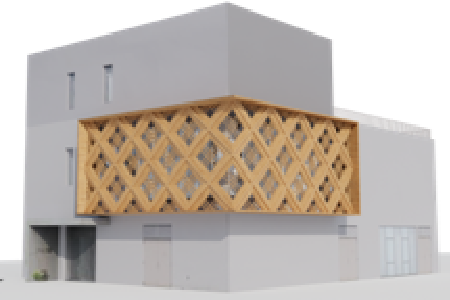
\includegraphics[width=1\linewidth]{Images/CICA3DRender1}} &
                    {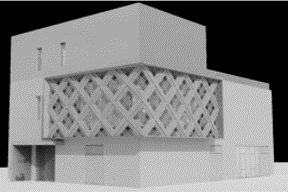
\includegraphics[width=1\linewidth]{Images/CICA3DRender2}} &
                  {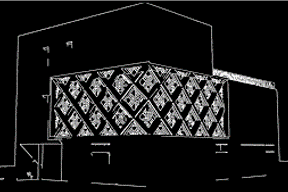
\includegraphics[width=1\linewidth]{Images/CICA3DRender3}} &
                  {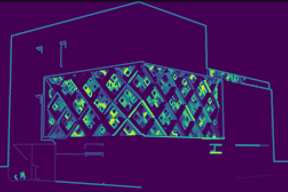
\includegraphics[width=1\linewidth]{Images/CICA3DRender4}} \\
                \midrule
                \text{(b) Historical Analysis} &  &  &
                \\
                {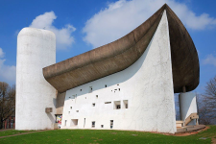
\includegraphics[width=1\linewidth]{Images/CICAHistory1}} &
                    {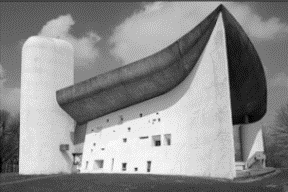
\includegraphics[width=1\linewidth]{Images/CICAHistory2}} &
                  {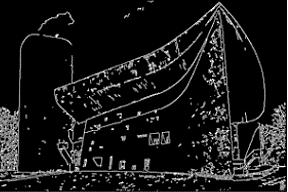
\includegraphics[width=1\linewidth]{Images/CICAHistory3}} &
                  {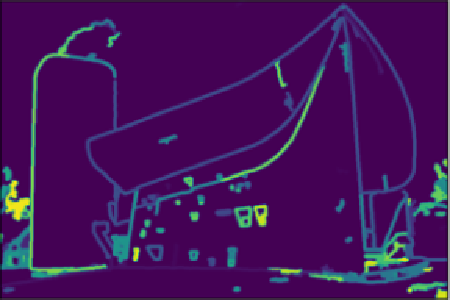
\includegraphics[width=1\linewidth]{Images/CICAHistory4}}\\
                \bottomrule
            \end{tabularx}
        \end{minipage}
    \end{tabular}
    \end{table*}

    %Cica scatter graph for renders
    \begin{table*}[htb]
    \centering
    \small
    \begin{tabular}{c}
        %Top cell with one figure
        %Scatter graph CICA renders
        \begin{minipage}{\textwidth}
        \centering
        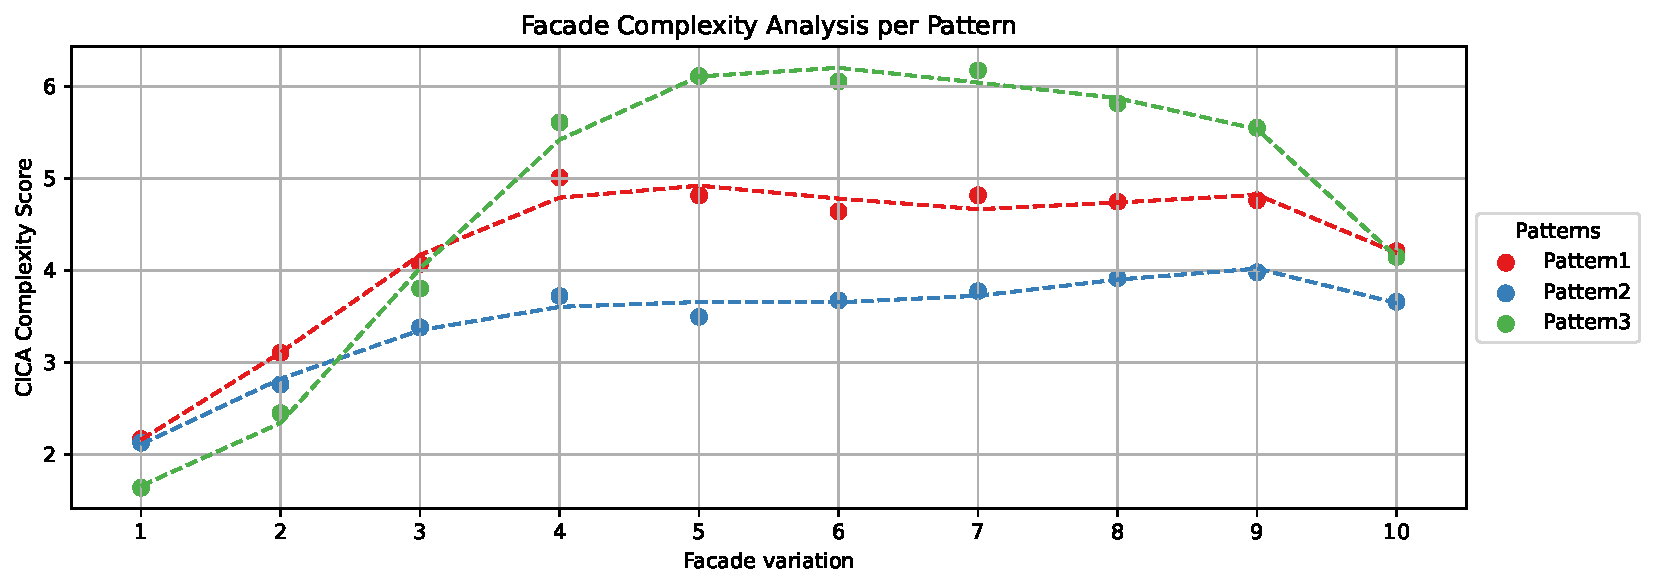
\includegraphics[width= \linewidth]{Graphs/complexitygraphrender}
        \captionof{figure}{Scatter Graph Analysis of 3d modeled Facade Complexity: This graph presents the CICA scores for ten variations of three distinct patterns created in Blender, with a trendline indicating the range of complexity levels among the facade designs, illustrating the nuanced relationship between design intricacy and CICA scores.}
        \label{fig:CICAscatterGraphRender}
        \end{minipage}
    \end{tabular}
    \end{table*}

    \subsubsection{3D Modeling and Environment setup}
    \label{subsubsec:3DModeling}
    %% description of things modeled in blender for use in the experiment
    %    \subsubsection{3D Modeling}
%    \label{subsubsec:Modeling}
%    %% description of things modeled in blender for use in the experiment
%    %    \subsubsection{3D Modeling}
%    \label{subsubsec:Modeling}
%    %% description of things modeled in blender for use in the experiment
%    \input{Text/3DModeling}

Ensuring a high level of realism is paramount in Virtual Reality simulation, particularly when aiming to replicate a genuine experience.
In the context of this research, our objective is to assess the reactions of individuals within a building adorned with facades of varying complexity.
Therefore, the precision of our 3D modeling is of utmost significance.

For this purpose, the ``3D modeling'' module realized in Blender (v3.6), serves as the first component and is responsible for generating the 3D models central to our research that include the site and building as a virtual environment where the experiment will be conducted and generating the distinctive facade variations.

The virtual environment created is an exact replica of the Architectural Environment Research Building, also known as Building HE20, which houses our laboratory on the Itoshima campus of Kyushu University (see Figure\ref{fig:RealVs3dModel}).

    %% Figure of Real building next to 3D modeled building
     \begin{figure}[t]
          \centering
          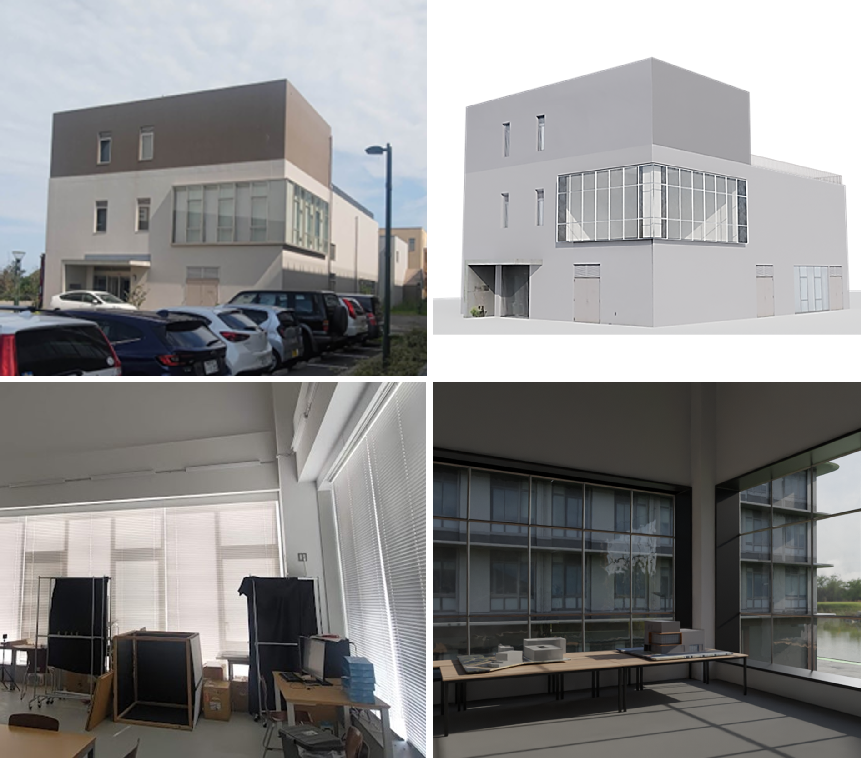
\includegraphics[width= \linewidth]{Images/Realvs3DmodelBlender}
          \caption{Side-by-side comparison of the Architectural Environment Building at Kyushu University used in the experiment, featuring actual interior and exterior photographs (left), and its virtual clone meticulously modeled and rendered in Blender (v3.6) for the Facade Design Complexity Analysis experiment.}
          \label{fig:RealVs3dModel}
        \end{figure}

To ensure an authentic experience, both the exterior of the building and the interior laboratory spaces were meticulously modeled to match the real-world dimensions.
This meticulous approach allows participants to seamlessly navigate the laboratory and revisit their initial encounters with the building's actual conditions, providing a basis for comparison with the virtual simulations.

With the building and its context successfully simulated, the next step was to establish a systematic workflow for creating facade variations with varying degrees of complexity (\ref{tab:PatternsVariationsPart0}).
Our first task was to identify the specific area of the building where the facade variations would be applied.
In Figure\ref{fig:RealVs3dModel}, you can observe that the laboratory's exterior walls feature two sizable windows facing the front and side of the building.
Remarkably, these windows align precisely with our laboratory space, granting an expansive view of a significant portion of the building's facade from inside the lab.

These large glazed surfaces became the central focus for simulating the facade variations.
They offer a unique opportunity for occupants of the laboratory to experience the facade changes firsthand, creating the sensation of being enveloped by the facade variations.
This approach ensures that participants in the experiment perceive a meaningful impact when the facades change from the interior of the lab, a perspective that would typically only be observed from a distance outside the building.

Once the area for applying the facade variations was identified, consisting of the two prominent windows with glazed curtain walls in the lab, the subsequent step was to extrapolate its base mesh and dimensions.
This formed the starting point for delineating the boundaries of the forthcoming building variations.

To enhance the experiment's diversity and variability in modeling facade variations, we chose to commence with three fundamental base patterns, as illustrated in Table\ref{tab:PatternsVariationsPart0} under the `Base Module' row.
These patterns drew inspiration from traditional Japanese motifs and served as the building blocks for creating ten distinct variations within each pattern, ensuring a comprehensive exploration of facade complexity in our study.

The generation of the ten facade variations involves a systematic process that incrementally accumulates complexity.
This progression from level 1 to level 10 is depicted in Table \ref{tab:PatternsVariationsPart0} under the 'Mesh per complexity level' column and is outlined as follows:

Levels 1 to 3: The base mesh is subdivided, creating smaller modules and increasing the pattern density on the facades.

Level 4: The subdivided mesh from level 3 undergoes a one-axis rotation, resulting in a tilted facade.

Level 5: The tilted facade is further bent along its central horizontal axis, forming a concave mesh.

Level 6: Curvature is applied alternately along the vertical axis, producing a wavy mesh.

Level 7: The previously waved mesh is vertically stretched at alternating points, resulting in variations in module size and spacing.

From Level 8 to Level 10: A decimation process is applied to the uniform mesh.
This process disrupts the uniformity of the mesh with minimal overall shape changes\cite{Blender2023}, achieved by collapsing edges.
This reduces the module count while increasing the randomness of the shape and orientation of the base pattern module, creating more complex and varied pattern configurations.

The decimation process is tuned with a \(20\%\) decimation rate for Level 8, \(40\%\) for level 9 and \(60\%\) for level 10.

Finally, the `3d modeling' component' is capable of generating renderings of each facade variation iteration for all three patterns chosen in this research to serve as input for the `Computational Image Complexity Analysis' (CICA) system.
These renderings serve a crucial role in verifying the complexity levels and establishing the ranking of complexity that will guide participants during the experiment.
By visually representing the facade variations, we ensure that the CICA system has the necessary data to evaluate and score the complexity of each iteration accurately.

With a comprehensive understanding of how the 3D modeling component supports the VR system, let's now delve into the application of the CICA system for ranking the 3D-modeled facades.
This process is integral to our Virtual Reality (VR) experiment, where participants will engage with facades featuring various complexity levels.



%
%To represent common challenges in site layout design, we selected three simulated sites (Table \ref{tab:SiteParametersAndPreview}), which included variations in slopes, gradients, and the need to preserve natural features. While these sites were fictitious, they were modeled based on the geographical properties of Fukuoka, Japan, where the experiment was conducted.
%
%The building in the simulation was designed to be photo-realistic (Figure \ref{fig:BuidlingSiteBlenderSimulation}) and served as a focal point for users to explore different positions on the terrain. The "optimization algorithm" of this system (see Figure \ref{fig:MOO_Flowchart}) extracted the building's dimensions, particularly its boundaries, to use them as input to define the building footprint and calculate its impact on the site during the Site Layout Planning process (Table \ref{tab:BuildingParameters}).

    %%Table: Pattern Variations sample 3, 6, 9
    \begin{table*}[htb]
        \centering
        \small
        \caption{Patterns variations for the First five levels of complexity}
        \label{tab:PatternsVariationsPart0}
        \begin{tabularx}
        {\textwidth}{p{4cm} >{\centering\arraybackslash}X >{\centering\arraybackslash}X >{\centering\arraybackslash}X }
            \toprule
            \textit{Description} &
              \textit{Pattern 1} &
              \textit{Pattern 2} &
              \textit{Pattern 3} \\
            \midrule
            \text{Pattern Name} & Hishi Pattern & Tortoise shells & Asanoha Pattern\\

            \midrule
            \textit{Base Module} &  &  &
            \\
            {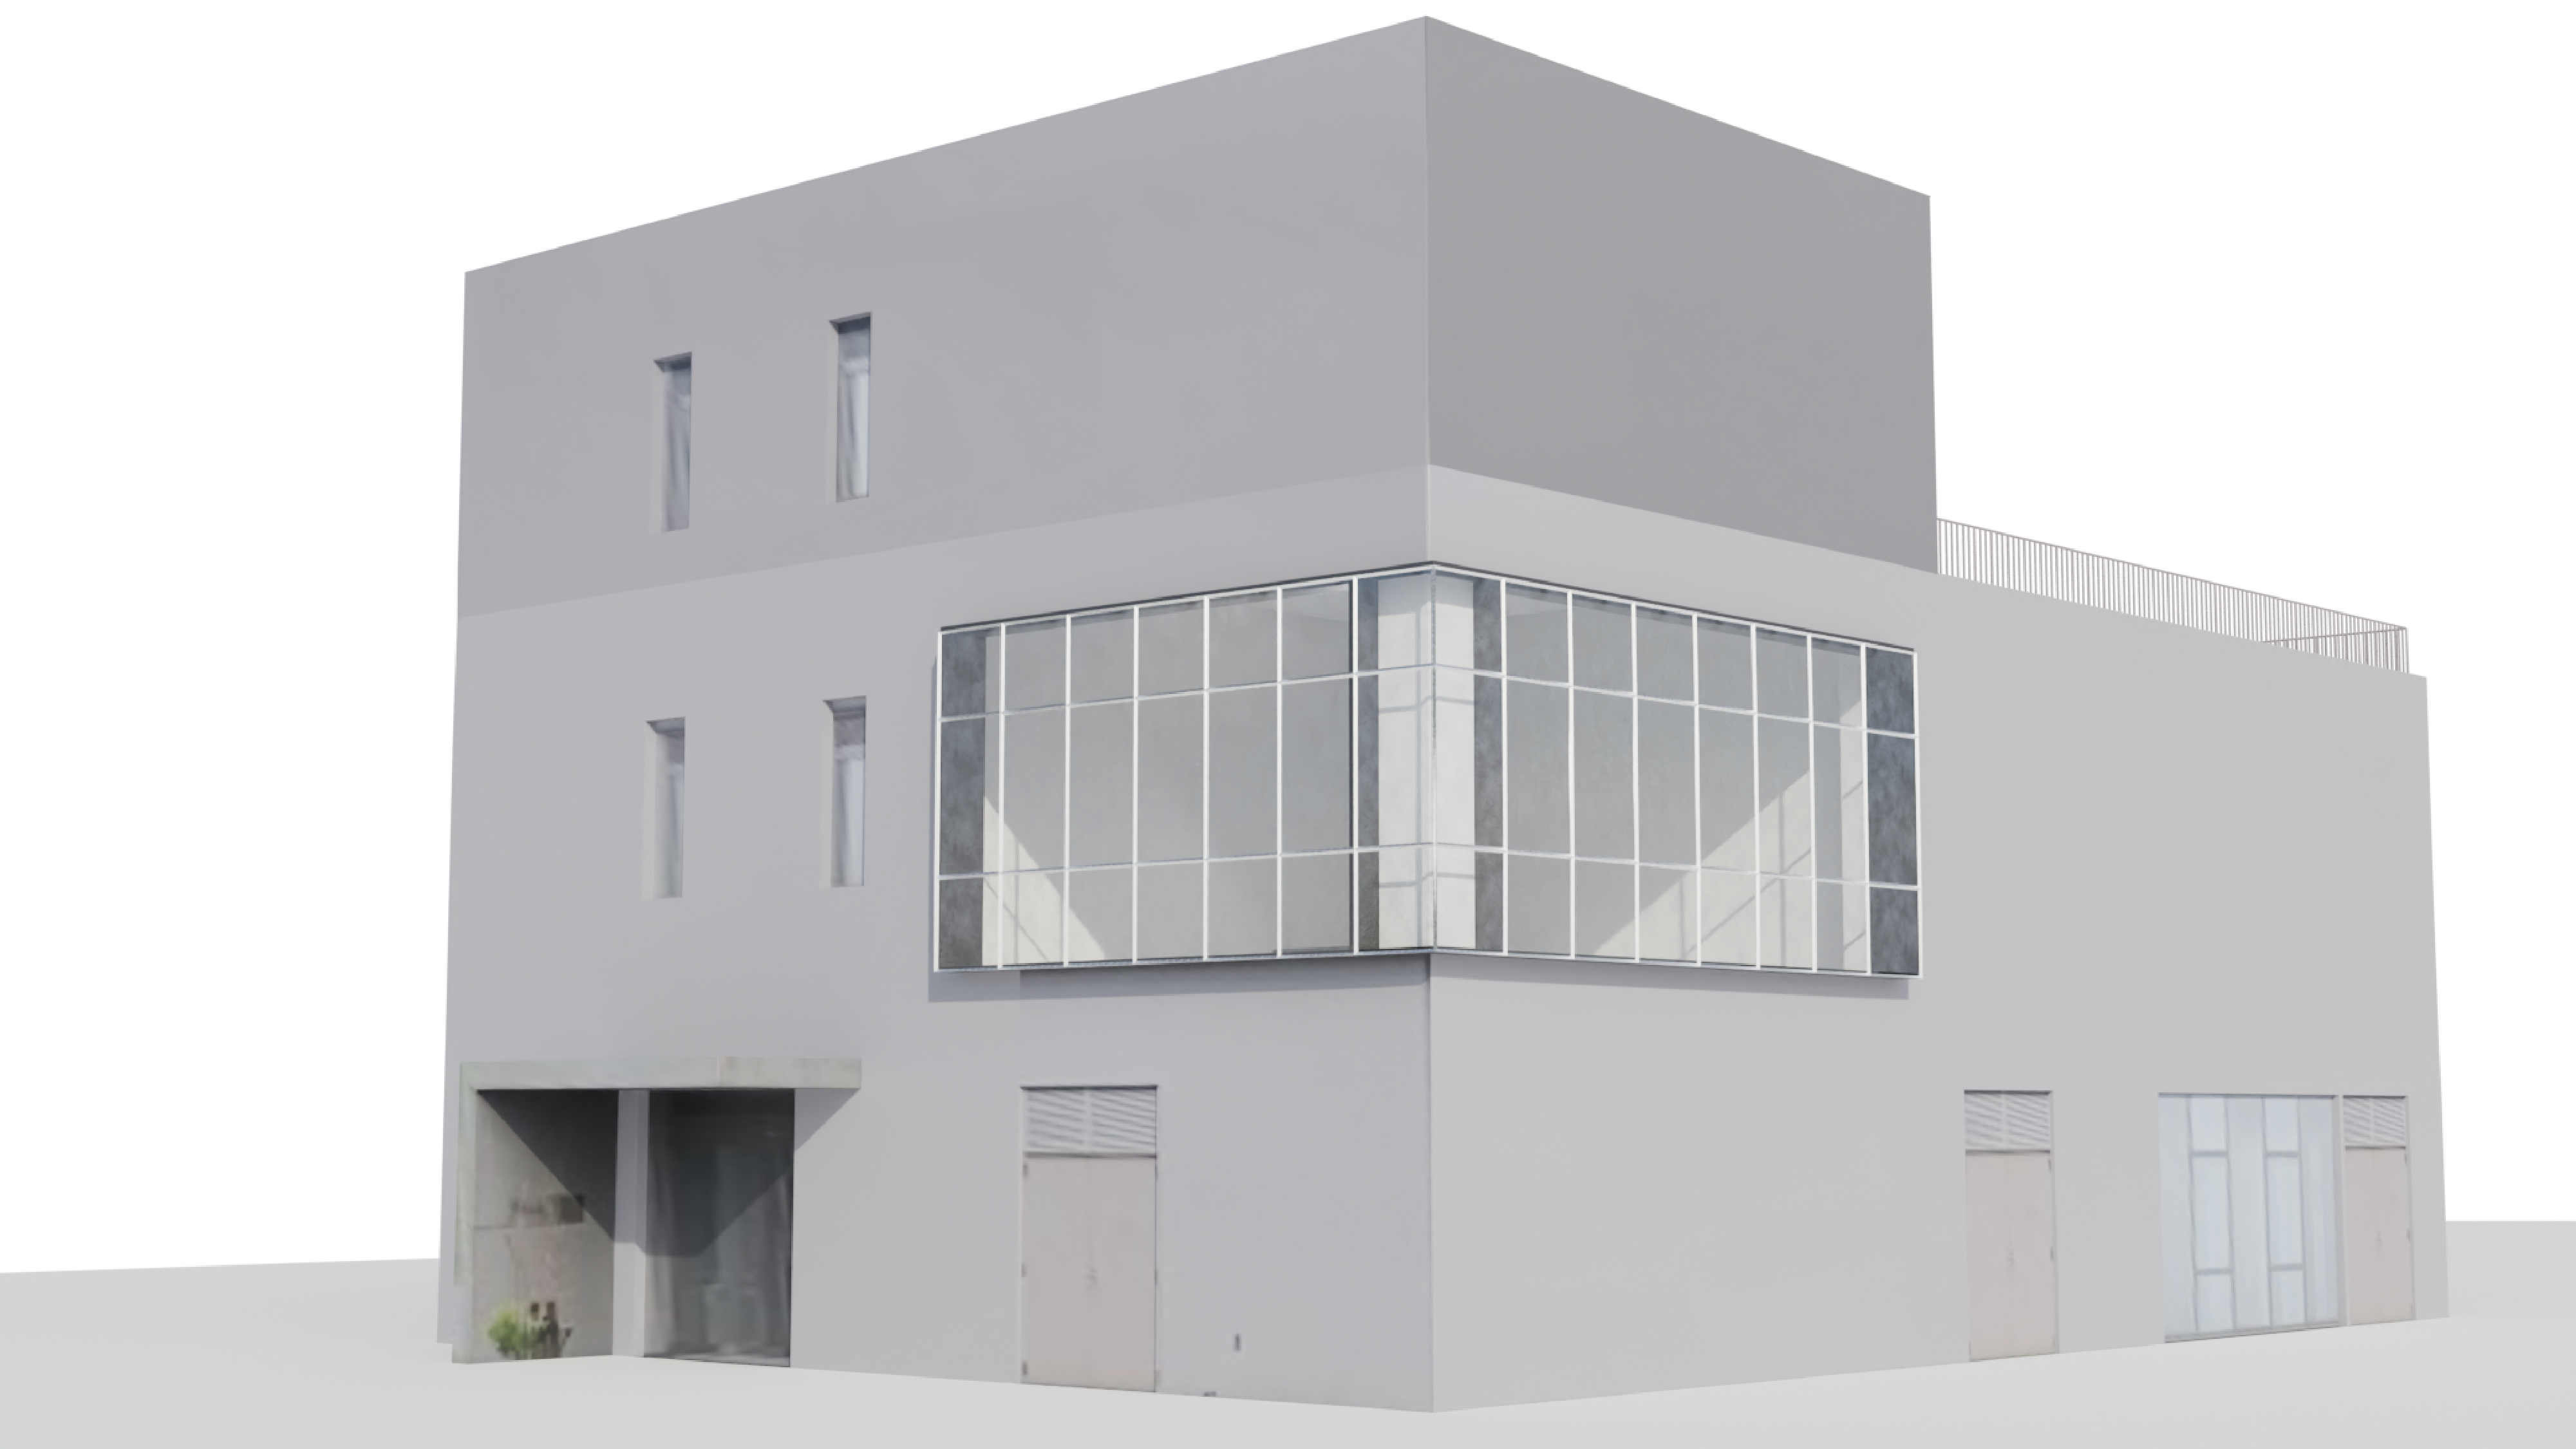
\includegraphics[width=1\linewidth]{Images/Base Module/Building}} &
              {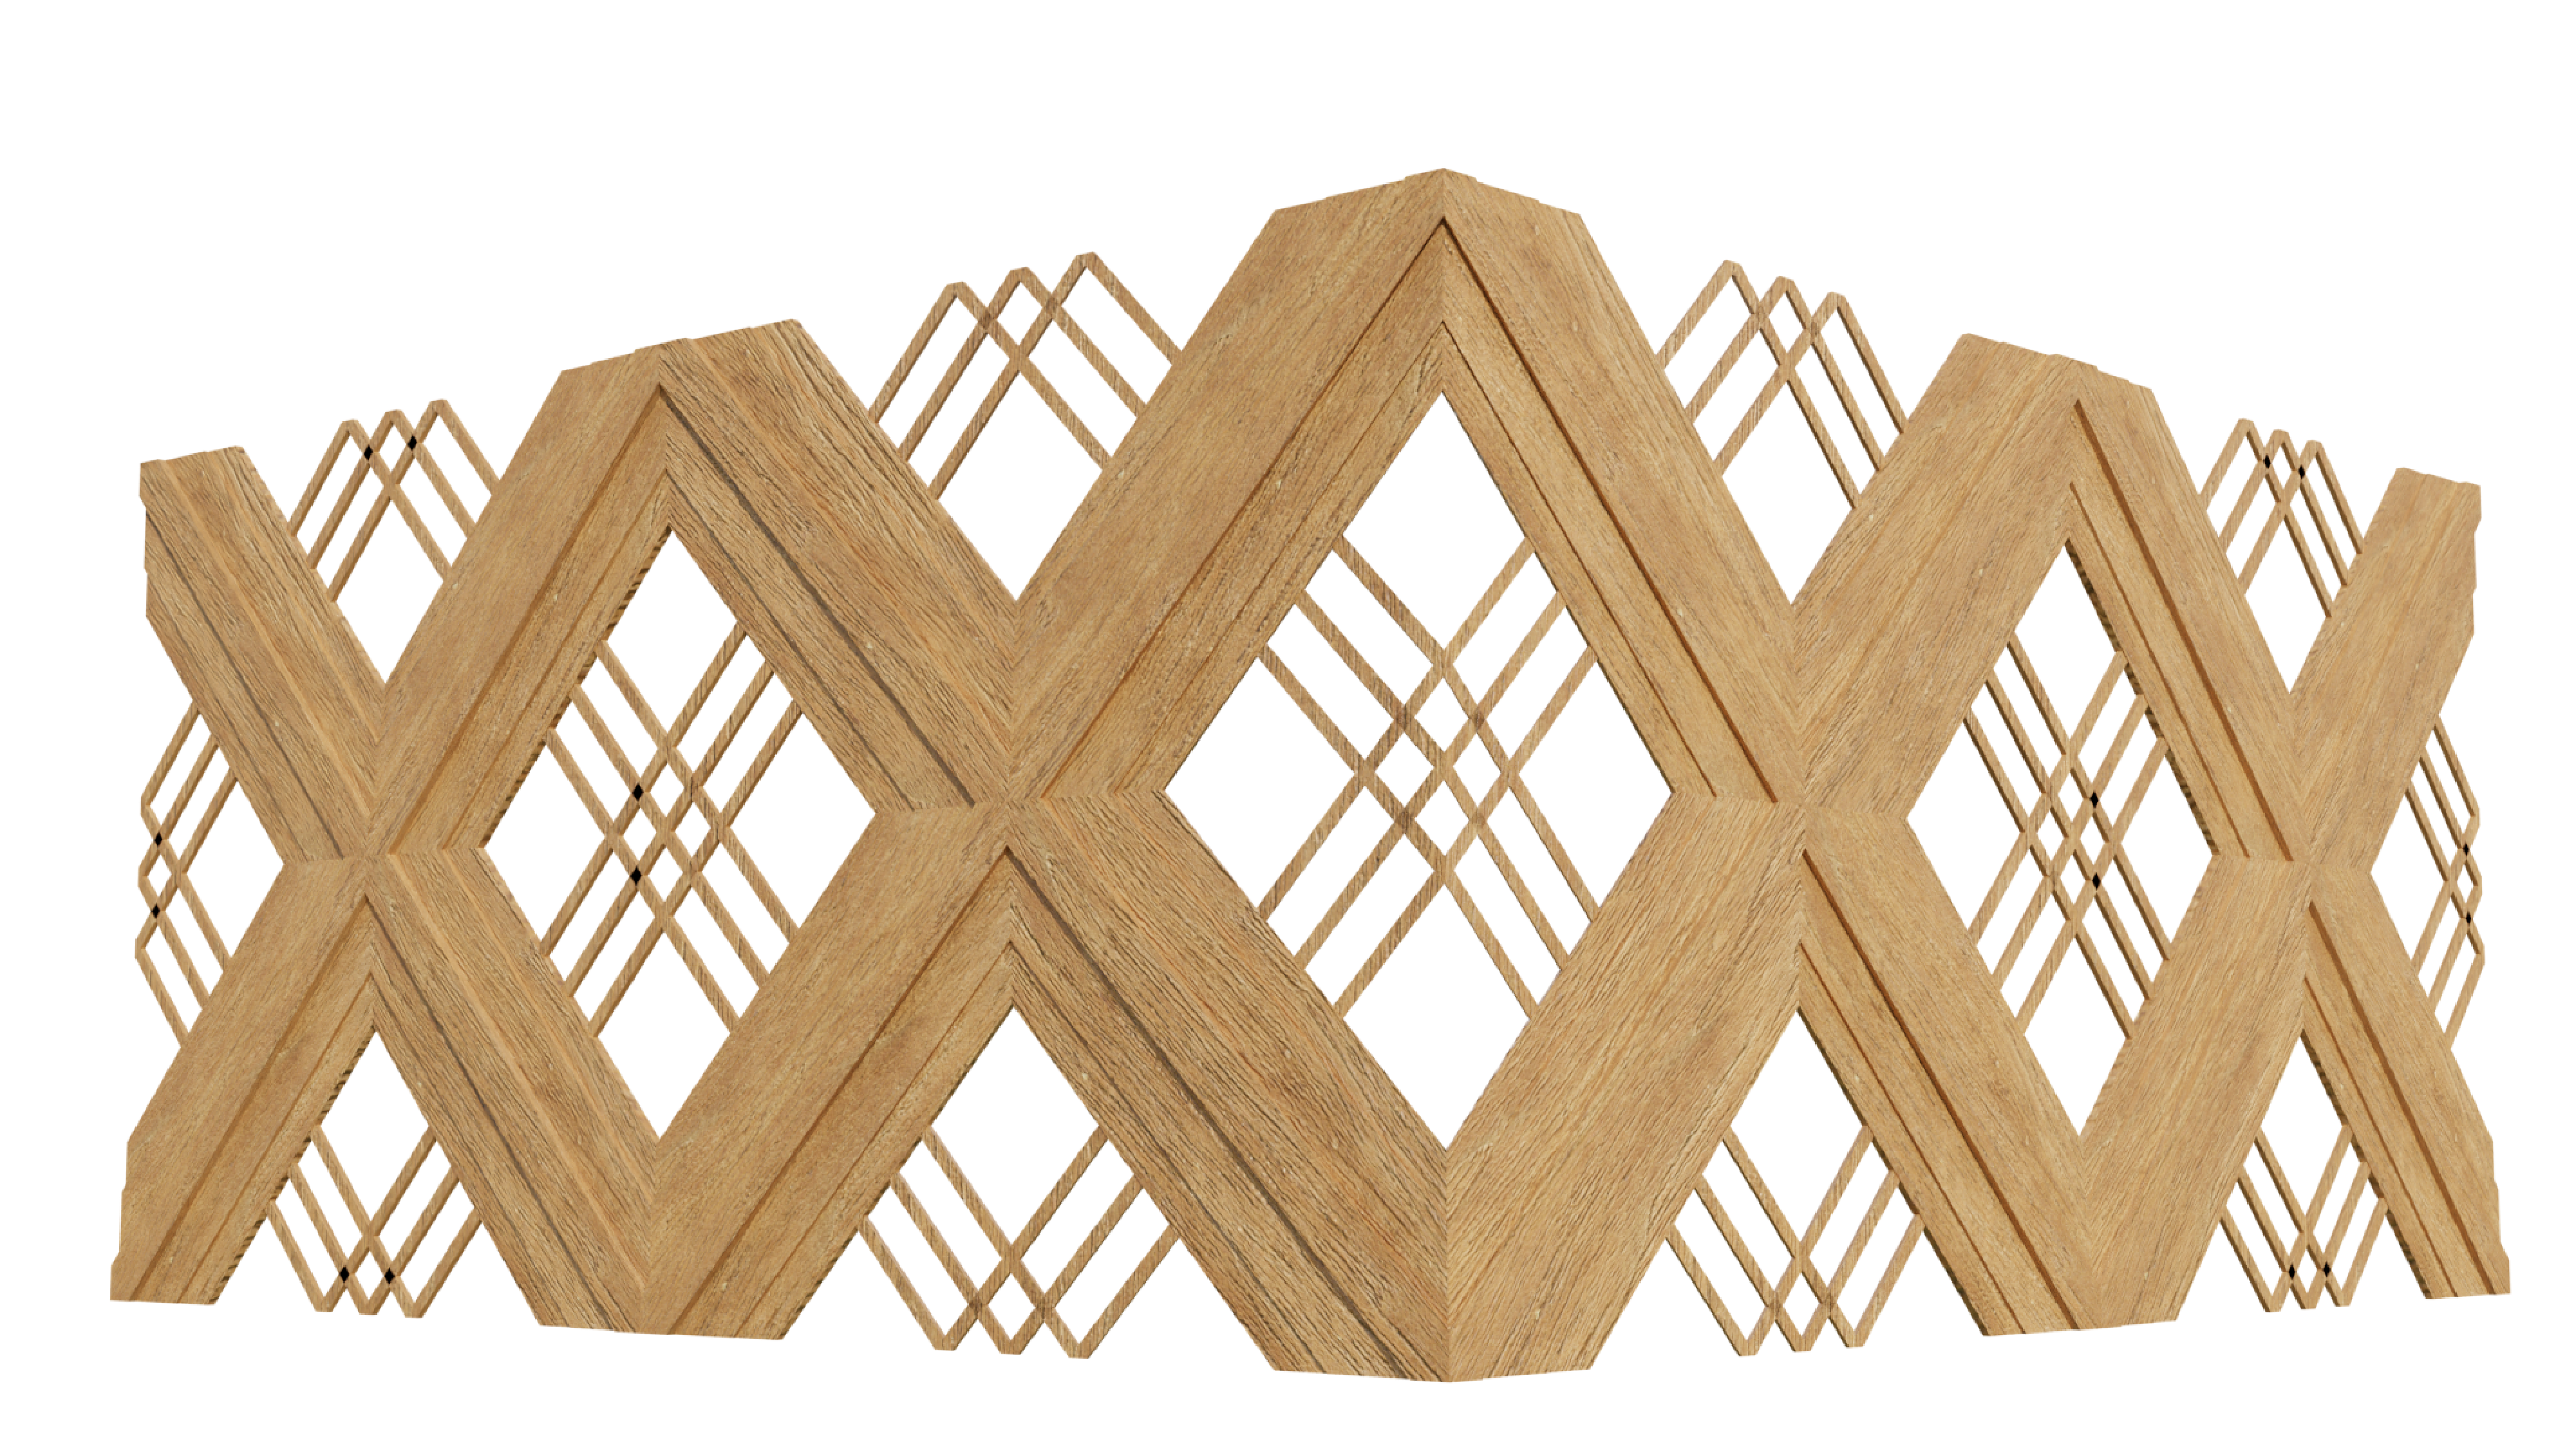
\includegraphics[width=1\linewidth]{Images/Base Module/Pattern1}} &
              {\includegraphics[width=1\linewidth]{Images/Base Module/Pattern2}} &
              {\includegraphics[width=1\linewidth]{Images/Base Module/Pattern3}} \\

            \midrule
            \textit{Mesh per complexity Level} &
              \textit{Pattern 1} &
              \textit{Pattern 2} &
              \textit{Pattern 3}\\

            \midrule
            \text{Level 3} &  &  &
            \\
            {\includegraphics[width=1\linewidth]{Images/Wall 0/0003}} &
              {\includegraphics[width=1\linewidth]{Images/Pattern 1/0003}} &
              {\includegraphics[width=1\linewidth]{Images/Pattern 2/0003}} &
              {\includegraphics[width=1\linewidth]{Images/Pattern 3/0003}} \\
            \midrule
            \text{Level 6} &  &  &
            \\
            {\includegraphics[width=1\linewidth]{Images/Wall 0/0006}} &
              {\includegraphics[width=1\linewidth]{Images/Pattern 1/0006}} &
              {\includegraphics[width=1\linewidth]{Images/Pattern 2/0006}} &
              {\includegraphics[width=1\linewidth]{Images/Pattern 3/0006}} \\
            \midrule
            \text{Level 9} &  &  &
            \\
            {\includegraphics[width=1\linewidth]{Images/Wall 0/0009}} &
              {\includegraphics[width=1\linewidth]{Images/Pattern 1/0009}} &
              {\includegraphics[width=1\linewidth]{Images/Pattern 2/0009}} &
              {\includegraphics[width=1\linewidth]{Images/Pattern 3/0009}} \\
            \bottomrule
        \end{tabularx}
    \end{table*}



%!Concise

To achieve realistic VR experiences for assessing user responses to facade complexity, a building site and facade variations were 3D modeled using Blender (v3.6).
Blender was selected for its advanced rendering capabilities, support for parametric and generative design, and seamless Python integration, necessary for integrating it with the CICA and VR components of the `Complexity Analysis' system.

The `building site' used for this study is a detailed virtual replica of the Architectural Environment Research Building at Kyushu University, Fukuoka-Japan, including both exterior and interior elements of the existing building (Figure~\ref{fig:modeling_flowchart}, elements [a] to [d]).~This building was chosen because it is the location where this study takes place, contributing significantly to the sense of immersion for participants during the experiment.

To test the response of occupants to various degrees of complexity, ten facade variations across three different patterns were 3D modeled and strategically placed over the large windows of the `building site' for maximum visual impact~(see Figure~\ref{fig:modeling_flowchart}, element [e] to [j]).

These patterns were selected to reflect a range of design approaches commonly seen in contemporary architecture—from minimalist to highly intricate facades reminiscent of Parametricism and Pragmatic Utopianism— representing current trends in modularity, geometric intricacy, and parametric design~\cite{Leach2016}. This ensures that the study captures a broad spectrum of facade styles relevant to contemporary architectural practices (see Figure~\ref{fig:contemporarytimeline} [d-e] in~\ref{sec:timeline-of-architectural-styles-across-history}).


The complexity of each facade variation was systematically increased by applying 3D modeling operations, from simple subdivisions to more advanced modifications such as rotations and decimation.
These operations simulate different levels of geometric intricacy that are reflective of real-world facade design challenges, such as material usage, constructability, and cost (Figure~\ref{fig:modeling_flowchart} (element [j] to [l])and further detailed in~\ref{sec:AnnexVariations}). Facades with higher mesh complexity represent designs that may demand more resources and construction time, making this aspect crucial for evaluating both aesthetic appeal and practical feasibility.
By varying the complexity levels, the study provides insight into how architectural complexity influences user perception and decision-making in facade design.

Each facade variation is rendered and labeled for use in the CICA complexity analysis, ensuring control over complexity variability.
This setup, provides a comprehensive environment for analyzing the accuracy of the `Complexity Analysis' system and investigating user perception.


%Achieving realistic 3D modeling is crucial for this study to replicate an authentic experience in VR, especially when assessing user responses to facade complexity.
%Using Blender (v3.6), our 3D modeling components creates a virtual replica of the Architectural Environment Research Building at Kyushu University, chosen as the experiment's set.
%This replica encompasses both exterior and interior details, as shown in Figure~\ref{fig:RealVs3dModel}.
%
%This component generates ten facade variations across three different patterns, positioned over the building's large windows for maximum visual impact (Figure~\ref{fig:VRInteriorExterior}). These 3 sets of variations, one for each pattern, are created systematically, with each level introducing greater complexity.
%The progression of complexity levels is illustrated in Table~\ref{tab:PatternsVariationsPart0} and fully detailed in~\ref{sec:AnnexVariations}.
%The operations for generating complexity, from base patterns in facade design, range from simple subdivision at the initial levels to more advanced modifications such as rotations, bends, and decimations at higher levels.
%
%Each variation is rendered and labeled for use in the CICA complexity analysis.
%This ensures control over the variability of complexity across the variations, using the CICA complexity score as a reference to guarantee diversity in the data pool of facades for the VR experiment.
%This diversity is evidenced in the scatter graph of facade complexity analysis per pattern in Figure~\ref{fig:CICAscatterGraphRender}.
%
%The 3D modeling component also includes a script for exporting these variations to FBX format, facilitating integration with the VR system.
%This detailed and systematic approach to 3D modeling ensures that the VR simulations accurately reflect real-world conditions, providing participants with a realistic and immersive experience during the experiment.









    \subsubsection{CICA System}
    \label{subsubsec:CICAsystem}
    % this section describes the computational image complexity analysis
%!Concise version

The literature review in Section~\ref{sec:LiteratureReview} revealed a cyclical nature in architectural evolution, alternating between complex and simple styles.
Our initial goal for the CICA system is to empirically validate these trends by developing a quantifiable scoring system capable of evaluating the complexity of historical and 3D-modeled building facades (Figure~\ref{fig:MethodologyFlowchartComplexity}, element 2).

Implemented as a Python script, the CICA system leverages Python's compatibility with Blender and its robust CV libraries, facilitating the integration of 3D models with complexity analysis scripts.

Inspired by Venturi et al.'s perspective on complexity~\cite{Venturi1977}, the CICA system measures complexity by the mental processing time required for a building's elements.
It uses two primary metrics: edge density and contour count, selected for their relevance to human vision's edge and object contour detection~\cite{Yang2022}.

\textit{Edge Density:} Utilizing the Canny Edge Detection algorithm~\cite{EdgeOpenCV2023}, this metric focuses on edge presence and density, defining architectural boundaries (Figure~\ref{fig:CICA_flowchart}, element (2) CICA process).
\deleted{(Table 1, column 3).}

\textit{Contour Count:} Using contour approximation techniques~\cite{ContourOpenCV2023}, this metric assesses shape intricacies outlined by edges (Figure~\ref{fig:CICA_flowchart}, element (3) CICA process).
\deleted{(Table 1, column 4).}

Both metrics are essential for shaping perceived complexity and are computationally efficient for large datasets~\cite{Yang2022}.

To quantify facade complexity from both metrics perspective, we employed a Multi-Objective Optimization (MOO) algorithm using the Analytic Hierarchy Process (AHP), a robust Multi-Criteria Decision-Making (MCDM) technique for detailed analysis and prioritization based on expert input and quantitative data~\cite{Taherdoost2023}.
The MOO algorithm is represented in the `Complexity Score' function \(f_1(x)\), defined in Equation~\ref{eq:F1_ComplexityScoreFunction1}, which normalizes the metrics and combines them into a `Unified Complexity Score':

\begin{equation}
    f_1(x) = \mathrm{round}\left(\sum_{i=1}^{n} w_i \cdot a_i, 2\right) = \text{complexity\_score}
    \label{eq:F1_ComplexityScoreFunction1}
\end{equation}

where \(n\) is the number of performance indicators, \(w_i\) is the weight of the \(i\)-th element, and \(a_i\) is the normalized score for the \(i\)-th metric (e.g., `Edge Density' and `Contour Count').
This weighted sum provides the overall complexity score or `CICA score' a quantifiable measure of facade complexity, crucial for the CICA system.

The CICA system has two main applications:
\begin{itemize}
    \item \textit{Historical Analysis:} Evaluates over 180 buildings from various architectural eras, creating a scatter graph of complexity scores organized by year and architecture style, showing complexity trends over time (Figure~\ref{fig:CICA_flowchart}[b]). Results are presented in Section~\ref{subsec:ResultsComplexityImageAnalysishistory}.\deleted{(Figure 4, element 2[b]; Table 3[b]).}

    \item \textit{3D-Modeled Facades Analysis:} Analyzes 10 facade variations across 3 patterns of 3D-modeled facades with varying complexity for the VR experiment (Figure~\ref{fig:CICA_flowchart}[a]). The CICA scores are used for comparison with user perceptions~(Figure~\ref{fig:CICAscatterGraphRender}).\deleted{(Figure 4, element 2[a]; Table 3[a]).}
\end{itemize}

Through these applications, the CICA system aims to validate architectural complexity trends empirically and prepare for experiments assessing user perceptions of facade complexity.


%!%Figures of VR integration
    %% Figure of VR interface
    \begin{table*}[htb]
        \centering
        \small
        \begin{tabular}{c}
            %Top cell
            % Optimization Flowchart
            \begin{minipage}{\textwidth}
                \centering
                  \includegraphics[width= \linewidth]{Images/VRInterface}
                \captionof{figure}{Detailed view of the VR interface (left) highlighting its five key sections: Viewpoint Navigation (1), Facade Variation Slider (2) for transitioning through ten facade variations, Facade Render Preview (3), Comparative Analysis Charts (4) displaying CICA complexity scores, and Utility Functions (5) for switching between the three patterns. Also shown are the VR simulations of the building's exterior (middle) and interior (right) as experienced during the facade complexity analysis, illustrating the transitions through various facade variations across all three patterns.}
                \label{fig:VRinterfaceComplexity}
            \end{minipage}
        \end{tabular}
    \end{table*}


    \subsubsection{VR integration and simulation tools}
    \label{subsubsec:VR_integration}
    %%Define the sections of the VR interface and how information is displayed
    %\subsubsection{VR integration and simulation tools}
%\label{subsubsec:VR_integration}
%%Define the sections of the VR interface and how information is displayed
%\input{Text/VR_integration}


The goal of this component is to integrate the virtual environment from the `3D Modeling and Environment Setup' with data from the CICA complexity analysis \deleted{(Figure 7)}(Figure~\ref{fig:MethodologyFlowchartComplexity}, element 3).
This module features an immersive `VR simulation' and a `data visualization interface' that allows users to explore and interact with the building's interior and exterior, visualize its context, and manipulate facade variations (element 3, Figure~\ref{fig:CICA_and_VR_flowchart}).

The `VR simulation,' was developed using Unity (v.2022.2.21f1) and accessible through a Head-Mounted Display (HMD), Oculus Quest 2.
This software was chosen for its robust VR support, pre-built templates, and seamless integration with Python and C\#, enhancing simulation interactivity and data handling.

%!Vr interface
The VR data visualization interface provides real-time feedback on facade variations, facilitating data collection on user response to varying levels of facade complexity.
Structured into five key sections—Viewpoint Navigation, Facade Variation Slider, Facade Render Preview, CICA Scores Comparative Analysis Charts, and Utility Functions \deleted{(labeled 1 to 5 in Figure 7)}(Figure~\ref{fig:CICA_and_VR_flowchart}, [e])—it enhances usability and interpretability, thereby optimizing the facade selection process.







    \subsection{Experiment Execution}
    \label{subsec:Experiment_execution}
    %%Task description, stage 1 to 3 with survey
    %\subsection{Experiment Execution}
%    \label{subsec:Experiment_execution}
%    %%Task description, stage 1 to 3 with survey
%    %\subsection{Experiment design}
%    \label{subsection:Experiment_design}
%    %%Task description, stage 1 to 3 with survey
%    \input{Text/ExperimentDesign}

%!text

The experiment assesses participants' reactions to complex facade variations in VR, using CICA-derived complexity data (element 3.2 in Figure~\ref{fig:MethodologyFlowchart}) and gathers their impression regarding evaluating facade complexity.
It consists of three stages:

%!VR interaction stage
\begin{enumerate}
    \item \textit{`VR interaction' stage:}  as illustrated in the flowchart in Figure~\ref{fig:MethodologyFlowchart}~(element 3.2 I), participants engage with a VR simulation of the actual laboratory and building where the experiment takes place (Figure~\ref{fig:VRinterface}). They select preferred facade variations from three patterns, each with ten complexity-labeled variations (Table~\ref{tab:PatternsVariationsPart0}) and data visualization of their CICA complexity score, considering the scenario as their permanent workplace or study location.
    Patterns are presented in randomized order to ensure unbiased results, accessible through the VR interface.

    \item \textit{`Screen-based Ranking' Stage:} As depicted in the flowchart in Figure~\ref{fig:MethodologyFlowchart}~(element 3.2 II), participants rank the same 10 facade variations based on their perception of complexity via a screen-based interface without CICA system data.
    This is conducted for each of the three patterns to refine the CICA system's complexity analysis capabilities.

    \item \textit{`Post-interaction' Survey:} As shown in the flowchart in Figure~\ref{fig:MethodologyFlowchart}~(element 3.2 III), after completing the first two stages, participants answer a 15-question survey divided into Participant Background (Figures~\ref{fig:SurveyBackgroundChart}~\ref{fig:SurveyYearsExperienceChart}) and Complexity Perception sections(Figures~\ref{fig:SurveyQuestions6-10}~\ref{fig:SurveyQuestions11-15}), exploring qualitative perceptions of complexity and the factors influencing their choices.
    This section uses a 7-point Likert scale for capturing detailed responses.
\end{enumerate}

%! Metrics purpose

The combined analysis of these stages aims to provide insights into user tolerance for complex facades and its implications for future construction trends.
By merging quantitative and qualitative findings, we contribute to the discourse on architectural complexity and its impact on contemporary design and construction.
%!text

The experiment assesses participants' reactions to complex facade variations in VR, using CICA-derived complexity data (element 3.2 in Figure~\ref{fig:MethodologyFlowchartComplexity}) and gathers their impression regarding evaluating facade complexity.
It consists of three stages:

%!VR interaction stage
\begin{enumerate}
    \item \textit{`VR interaction' stage:}  as illustrated in the flowchart in Figure~\ref{fig:Experiment_flowchart}~(element 3.2 I) \deleted{Figure 4 (element 3.2 I)}, participants engage with a VR simulation of the actual laboratory and building where the experiment takes place \deleted{(Figure 7)} (see Figure~\ref{fig:CICA_flowchart}, element 3). They select preferred facade variations from three patterns, each with ten complexity-labeled variations (Figure~\ref{fig:modeling_flowchart}) and data visualization of their CICA complexity score, considering the scenario as their permanent workplace or study location.
    Patterns' variations are presented in randomized order to ensure unbiased results, accessible through the VR interface.

    \item \textit{`Screen-based Ranking' Stage:} As depicted in the flowchart in Figure~\ref{fig:Experiment_flowchart}~(element 3.2 II) \deleted{Figure 4 (element 3.2 II)}, participants rank the same 10 facade variations based on their perception of complexity via a screen-based interface without CICA system data.
    This is conducted for each of the three patterns to refine the CICA system's complexity analysis capabilities.

    \item \textit{`Post-interaction' Survey:} As shown in the flowchart in Figure~\ref{fig:Experiment_flowchart}~(element 3.2 III)\deleted{Figure 4 (element 3.2 III)}, after completing the first two stages, participants answer a 15-question survey divided into Participant Background (Figures~\ref{fig:SurveyBackgroundChart}~\ref{fig:SurveyYearsExperienceChart}) and Complexity Perception sections(Figures~\ref{fig:SurveyQuestions6-10}~\ref{fig:SurveyQuestions11-15}), exploring qualitative perceptions of complexity and the factors influencing their choices.
    This section uses a 7-point Likert scale for capturing detailed responses.
\end{enumerate}

%! Metrics purpose

The combined analysis of these stages aims to provide insights into user tolerance for complex facades and its implications for future construction trends.
By merging quantitative and qualitative findings, we contribute to the discourse on architectural complexity and its impact on contemporary design and construction.


    %!Table CICA scatter graph and table of Top and bottom scores for buildings
    % Table with figures and data from top 5 and bottom 5 CICA complexity scores of buildings from historical analysis
    \begin{table*}[!htb]
    \centering
    \small
    \begin{tabular}{c}
        %Top cell with one figure
        %Figure: CICA scatter graph for historical analysis
        \begin{minipage}{\textwidth}
            \centering
            \includegraphics[width= \linewidth]{Graphs/complexitygraph}
            \captionof{figure}{Scatter Graph of Architectural Complexity Over Time: This graph presents the CICA scores for 177 buildings, categorized by historical timeline and architectural style. An overlaid trendline highlights the current evolving trend towards increased complexity in architectural design as analyzed by the CICA system.}
            \label{fig:HistoricalComplexityGraph}
        \end{minipage}
        \\
        \\
        %2nd row with one table
        %Table: CICA top 5 buildings with year and scores
        \begin{minipage}{\textwidth}
            \centering
            \captionof{table}{Table of comparative CICA Historical Analysis results: Top 5 Highest and Bottom 5 Lowest CICA Complexity Scores from Historical Analysis, Including Year of Construction and Architectural Style.}
            \label{tab:Top5andBottom5CICAcomplexityScores}
            \begin{tabularx}{\linewidth}{c X c c c}
            \toprule
            \multicolumn{5}{c}{\textbf{Buildings with the Top 5 Highest CICA Complexity Scores}} \\
            \hline
            \textbf{Rank} & \textbf{Building Name} & \textbf{Year of Construction} & \textbf{Architectural Style} & \textbf{CICA Score} \\
            \hline
            1 & Westminster Abbey & 1245 & Gothic & 7.81 \\
            2 & Seattle Central Library & 2004 & Deconstructivism & 7.78 \\
            3 & Reims Kathedrale & 1275 & Gothic & 7.51 \\
            4 & California Academy of Sciences & 2008 & Hightech Modernism & 7.45 \\
            5 & Rome Trevi Fountain & 1732 & Baroque & 7.39 \\
            \hline
            \end{tabularx}
        \end{minipage}
        \\
        \\
        %3rd row cell with Figure
        %Figure CICA top 5 buildings
        \begin{minipage}{\textwidth}
            \centering
            \includegraphics[width= \linewidth, trim=0cm 0.5cm 0cm 0.5cm]{Images/CICATop5}
            \label{fig:CICATop5scores}
        \end{minipage}
        \\
        %4rd row cell with Table
        %Table: CICA bottom 5 buildings with year and scores
        \begin{minipage}{\textwidth}
            \centering
            \begin{tabularx}{\linewidth}{c X c c c}
            \hline
            \multicolumn{5}{c}{\textbf{Buildings with the Bottom 5 Lowest CICA Complexity Scores}} \\
            \hline
            \textbf{Rank} & \textbf{Building Name} & \textbf{Year of Construction} & \textbf{Architectural Style} & \textbf{CICA Score} \\
            \hline
            1 & Luce Memorial Chapel, Taichung City, Taiwan & 1963 & Modernism & 0.66 \\
            2 & Imperial War Museum North & 2002 & Deconstructivism & 0.79 \\
            3 & St. Mary's Cathedral, Tokyo & 1964 & Modernism & 1.07 \\
            4 & Disney Concert Hall & 2003 & Deconstructivism & 1.13 \\
            5 & Cathedral of Brasilia in Brazil & 1970 & Modernism & 1.22 \\
            \bottomrule
            \end{tabularx}
        \end{minipage}
        \\
        \\
        %Bottom cell with Figure
        %Figure CICA top 5 buildings
        \begin{minipage}{\textwidth}
            \centering
            \includegraphics[width= \linewidth, trim=0cm 0.5cm 0cm 0.5cm]{Images/CICABottom5}
            \label{fig:CICABottom5scores}
        \end{minipage}
    \end{tabular}
    \end{table*}

    \subsection{Data Analysis and Validation}
    \label{subsec:Data_analysis}
    %\subsection{Data Analysis and Validation}
%    \label{subsec:Data_analysis}
%    The final phase of our methodology involves a detailed analysis of the data collected during the experiments, crucial for validating the effectiveness of the `Complexity Analysis' system in evaluating facades.

It is structured as follows:

\begin{enumerate}
    \item \textit{Data Processing and Analysis:} ...Advanced statistical tools
    \item \textit{Performance Evaluation:} We assess the `Complexity Analysis' system's impact on user by examining:
        \begin{itemize}
            \item \textit{Accuracy Analysis:} ...
            \item \textit{Participant Perception Survey:} ...
        \end{itemize}

        These metrics are critical

    \item \textit{Results Interpretation and Reporting:} Data synthesis ...
\end{enumerate}

%Closing statement

%

The final phase of our methodology focuses on analyzing the data collected during the experiments and the application of the CICA system to images of historical buildings, aiming to validate the effectiveness of the `Complexity Analysis' system in quantifying facade complexity and aligning it with user perceptions (see Figure~\ref{fig:Experiment_and_Data_Analysis_flowchart}, element 3.3).

\textit{Data Processing and Analysis:} We assess CICA scores from historical buildings to identify patterns across different architectural styles and analyze experiment data using statistical tools to understand perceptions of complexity.

\textit{Performance Evaluation:} The efficacy of the `Complexity Analysis' system and the CICA score is assessed through:
\begin{itemize}
    \item \textit{Accuracy Analysis:} Evaluating the alignment between CICA scores and user perceptions.
    \item \textit{Participant Perception:} Analyzing user feedback to gain insights into the impact of complex facades.
\end{itemize}

\textit{Results Interpretation and Reporting:} Synthesizing data to confirm the validity of the CICA system and its applicability in architectural design.

While the primary focus of this phase is on validating the CICA system’s ability to quantify complexity, the combined analysis of historical architectural trends and real-time user perceptions provides potential insights into future construction trends.
By comparing these historical trends with user preferences gathered in the VR experiment, the CICA system provides a framework for predicting future design shifts.
Additionally, through the system’s ability to conduct accuracy analysis, architects could better identify the optimal range of complexity that appeals to users, allowing for the design of facades that align with predicted trends while balancing aesthetic interest and functional sustainability.
Over time, as more data is gathered, the CICA system's predictive capabilities could offer architects valuable foresight into emerging trends in facade design that might become prominent in future construction practices.

This structured approach ensures a thorough evaluation, providing insights into the relationship between facade complexity and user perception.









\section{Results and Discussion}
\label{sec:Results}
%% Results should be clear and concise.
%!\section{Results}
%\label{sec:Results}
%%!\section{Results}
%\label{sec:Results}
%\input{text/RD_1Results_DiscussionIntro.tex}

%=============================
%%% Results should be clear and concise.
%Report the results of the study
%Report main findings concisely in a logical order

% Intro ===============

Building upon the methodologies outlined in the previous sections, this section presents findings from two primary sources: the application of the CICA system to a historical dataset of architectural images across various epochs and styles, and data collected from the experiment designed to gauge user responses to facade complexity.
Organized according to the goals set forth in the introduction, this section elucidates the evolving relationship between users and architectural complexity, providing valuable insights for future construction practices and the quantification of complexity in facade design.


%!Goals oriented discussion


%\begin{itemize}
%    \item Analyze historical architectural trends to discern the oscillation between complexity and simplicity.
%    \item {Apply the CICA system to quantitatively assess facade complexity across architectural eras.}
%    \item {Utilize VR to measure user tolerance and preference for complexity in facade design.}
%    \item \textbf{Investigate the alignment of user preferences with current trends in the AEC industry, especially concerning digital fabrication.}
%    \item \textbf{Provide actionable insights on the future of architectural design and construction, guided by empirical data on user preferences and technological capabilities.}
%\end{itemize}





%=============================
%%% Results should be clear and concise.
%Report the results of the study
%Report main findings concisely in a logical order

% Intro ===============

Building upon the methodologies outlined in the previous sections, this section presents findings from two primary sources: the application of the CICA system to a historical dataset of architectural images across various epochs and styles, and data collected from the experiment designed to gauge user responses to facade complexity.
Organized according to the goals set forth in the introduction, this section elucidates the evolving relationship between users and architectural complexity, providing valuable insights for future construction practices and the quantification of complexity in facade design.


%!Goals oriented discussion


%\begin{itemize}
%    \item Analyze historical architectural trends to discern the oscillation between complexity and simplicity.
%    \item {Apply the CICA system to quantitatively assess facade complexity across architectural eras.}
%    \item {Utilize VR to measure user tolerance and preference for complexity in facade design.}
%    \item \textbf{Investigate the alignment of user preferences with current trends in the AEC industry, especially concerning digital fabrication.}
%    \item \textbf{Provide actionable insights on the future of architectural design and construction, guided by empirical data on user preferences and technological capabilities.}
%\end{itemize}





    \subsection{Assessment and Implications of Facade Complexity across Architectural Eras using the CICA System and insights from literature review}
    \label{subsec:ResultsComplexityImageAnalysishistory}
    %!\subsection{Assessment and Implications of Facade Complexity across Architectural Eras using the CICA System and insights from literature review}
%    \label{subsec:ResultsComplexityImageAnalysishistory}
%    %!\subsection{Quantitative complexity Analysis}
%    \label{subsec:ComplexityImageAnalysis}
%    \input{Text/RD_ResultsCICAHistory.tex}
%% Figure of Complexity graph

We have previously discussed that architectural evolution has been characterized by a continual interplay between simplicity and complexity.
Our literature review, presented in Section \ref{sec:Literature review}, has consistently pointed towards a prevailing trend in contemporary architecture, suggesting a resurgence of complexity in architectural design.

Our initial hypothesis, grounded in a rigorous examination of architectural styles from a theoretical standpoint, detailed in Section \ref{subsec:TimelineArchitectureStyles}, suggests that architecture undergoes cyclical oscillations between simplicity and complexity.
In the post-modern era, we posited that contemporary architecture would witness a resurgence of complexity and ornamentation.
This resurgence is exemplified by the emergence of five prominent styles: Deconstructivism, Neofuturism, High-tech Modernism, Parametricism, and Pragmatic Utopianism (see Figure \ref{fig:contemporarytimeline}).

These styles are influenced by technological advancements, the widespread use of computer-aided design tools, and a growing focus on sustainability.
Together, these factors contribute to a contemporary architectural landscape characterized by increasing complexity.

\textbf{CICA System for Quantitative Assessment}

While defining architectural complexity is inherently challenging due to its interconnection with various socio-economic factors influencing urban development, the development of the CICA system was based on a premise.
By accumulating a vast and diverse dataset of architectural works from different centuries, we aimed to uncover discernible patterns that would validate our hypothesis: architecture is characterized by a continuous dialogue between simplicity and complexity, with a trend towards increased complexity in contemporary architecture.

To objectively validate this trend, we conducted a quantitative analysis using the CICA system.
This rigorous analysis method utilizes input images of the most iconic and representative buildings from various epochs and styles, totaling 177 buildings across 14 architectural styles(illustrated in timelines in Figure \ref{fig:Oldtimeline}, \ref{fig:Middletimeline}, \ref{fig:contemporarytimeline}).
The CICA system took only 4.54 seconds to calculate the CICA scores for all the buildings and plot the graph, demonstrating its efficiency for complexity analysis.

The results are visually depicted in the scatter graph titled `Architectural Complexity over time' in Figure \ref{fig:HistoricalComplexityGraph}, and a 9th-degree polynomial trendline was found to be the best fit due to its versatility in accommodating the intricate data patterns that naturally emerge when assessing historical building complexity scores, the outcome of this choice was the emergence of a curve characterized by an intriguing cyclic pattern.

The distinctive pattern found on the trendline, akin to an undulating curve, uncovers a continual oscillation between architectural complexity and simplicity.
It resembles the paradigmatic shifts in architectural design discussed within our theoretical analysis (see section\ref{subsec:FacadeandOrnament}), a phenomenon that has endured throughout architectural history.

\textbf{Periods of Rapid Change:}
The polynomial curve in the 'Historical Complexity Analysis' Chart (Figure \ref{fig:HistoricalComplexityGraph}) reveals a dynamic oscillation between periods of ornamental richness and minimalist restraint, illustrating the unique interpretation of architectural complexity in each historical era.

Notably, the late 20th century show spikes in complexity scores, indicating significant shifts in architectural trends associated with the transition from the minimalist aesthetics of Modernism to the more eclectic and elaborate designs of Postmodernism.
Additionally, a shift is observed from the Gothic to the Renaissance period, where the trendline peaks with the ornate and vertical architecture of the Gothic era and descends as the Renaissance favors harmony, proportion, and classical simplicity \cite{Stacbond2020}.

Furthermore, our analysis of the last 50 years of data reveal an upward trajectory in architectural complexity, marking a departure from the minimalism of the 1950s and 1960s Modernist movement.
This trend supports our hypothesis and underscores the cyclical nature of architectural complexity, reflecting ongoing dialogues within architectural practice throughout history.

\textbf{Outliers:} Certain buildings stand out with exceptionally high or low complexity scores, warranting individual examination to understand their unique design elements or historical context.
Our investigation into the extremes of architectural complexity, as evidenced by the top 5 highest and bottom 5 lowest CICA scores (refer to Table \ref{tab:Top5andBottom5CICAcomplexityScores}), reveals significant outliers that deviate from the predominant complexity trends identified in our historical analysis.

Westminster Abbey, constructed in 1245 and exemplifying the Gothic architectural style, tops the chart with the highest CICA complexity score of 7.81 (Table \ref{tab:Top5andBottom5CICAcomplexityScores}, Top (1)).
This result underscores the intricate design characteristic of the Gothic period, known for its detailed stonework and skyward designs\cite{Stacbond2020}.

Conversely, the Luce Memorial Chapel in Taichung City, Taiwan, represents the other extreme, obtaining the lowest CICA complexity score of 0.66.
Built in 1963, this Modernist building exemplifies the minimalist ethos of the time, focusing on simplicity and functionality(Table \ref{tab:Top5andBottom5CICAcomplexityScores}, Bottom (1)).

These two buildings, marking the highest and lowest complexity scores in our study, illustrate the broad spectrum of architectural styles and the associated complexity over time and serve as critical case studies for understanding the factors that drive exceptional complexity or simplicity in architectural design.

%%Continue here

%\textbf{Correlation with Historical Events:} The complexity trends appear to correlate with major historical events, such as the industrial revolution and the advent of digital design technologies, influencing architectural design approaches.

%!Gothic Period
%Medieval Period (12th to 16th Century): Gothic architecture emerged in the High and Late Middle Ages, a time characterized by a growth in population, trade, and the establishment of universities. The period saw a shift from the Romanesque style to the Gothic style, which was marked by innovations such as the pointed arch, ribbed vault, and flying buttress. These architectural advancements allowed for taller, more light-filled structures, which were often used in the construction of cathedrals and churches.
%
%Crusades (11th to 13th Century): The Crusades played a role in the cultural exchange between the East and West. The exposure to Eastern architectural styles and techniques may have influenced the development of Gothic architecture in Europe. The increased wealth from trade and the need for monumental religious structures to demonstrate piety and power also contributed to the flourishing of Gothic architecture.


%!Renaissance
%Enlightenment (Illuminism) (Late 17th to 18th Century): This period emphasized reason, science, and individualism, which could have influenced a shift towards more rational and less ornate architectural designs.

%!Neo-classical and eclectic naturalism
%Industrial Revolution (Late 18th to Early 19th Century): The advent of new building materials like iron and steel, along with advancements in construction techniques, enabled more complex and innovative architectural designs.

%!International style and modernism
%World War I (1914-1918) and World War II (1939-1945): The wars and their aftermaths led to a focus on functionality and austerity in architecture, contributing to the rise of Modernism and its emphasis on simplicity.

%!Post modernism and contemporar styles
%Advent of Computers (Mid-20th Century Onwards): The introduction of computer-aided design (CAD) tools allowed architects to explore more complex and intricate designs, contributing to the rise of styles like Deconstructivism and Parametricism.
%
%Post-Industrialization and Globalization (Late 20th to Early 21st Century): These phenomena have led to a more interconnected world, with a diverse range of architectural styles and a trend towards complexity in design to accommodate new urban and environmental challenges.










%% Figure of Complexity graph

We have previously discussed that architectural evolution has been characterized by a continual interplay between simplicity and complexity.
Our literature review, presented in Section~\ref{sec:LiteratureReview}, has consistently pointed towards a prevailing trend in contemporary architecture, suggesting a resurgence of complexity in architectural design.

Our initial hypothesis, grounded in a rigorous examination of architectural styles from a theoretical standpoint, detailed in Section~\ref{subsec:TimelineArchitectureStyles}, suggests that architecture undergoes cyclical oscillations between simplicity and complexity.
In the post-modern era, we posited that contemporary architecture would witness a resurgence of complexity and ornamentation.
This resurgence is exemplified by the emergence of five prominent styles: Deconstructivism, Neofuturism, High-tech Modernism, Parametricism, and Pragmatic Utopianism (see Figure~\ref{fig:contemporarytimeline}).

These styles are influenced by technological advancements, the widespread use of computer-aided design tools, and a growing focus on sustainability.
Together, these factors contribute to a contemporary architectural landscape characterized by increasing complexity.

\textbf{CICA System for Quantitative Assessment}

While defining architectural complexity is inherently challenging due to its interconnection with various socio-economic factors influencing urban development, the development of the CICA system was based on a premise.
By accumulating a vast and diverse dataset of architectural works from different centuries, we aimed to uncover discernible patterns that would validate our hypothesis: architecture is characterized by a continuous dialogue between simplicity and complexity, with a trend towards increased complexity in contemporary architecture.

To objectively validate this trend, we conducted a quantitative analysis using the CICA system.
This rigorous analysis method utilizes input images of the most iconic and representative buildings from various epochs and styles, totaling 177 buildings across 14 architectural styles(illustrated in timelines in Figure~\ref{fig:Oldtimeline},~\ref{fig:Middletimeline},~\ref{fig:contemporarytimeline}).
The CICA system took only 4.54 seconds to calculate the CICA scores for all the buildings and plot the graph, demonstrating its efficiency for complexity analysis.

The results are visually depicted in the scatter graph titled `Architectural Complexity over time' in Figure~\ref{fig:HistoricalComplexityGraph}, and a 9th-degree polynomial trendline was found to be the best fit due to its versatility in accommodating the intricate data patterns that naturally emerge when assessing historical building complexity scores, the outcome of this choice was the emergence of a curve characterized by an intriguing cyclic pattern.

The distinctive pattern found on the trendline, akin to an undulating curve, uncovers a continual oscillation between architectural complexity and simplicity.
It resembles the paradigmatic shifts in architectural design discussed within our theoretical analysis (see section\ref{subsec:FacadeandOrnament}), a phenomenon that has endured throughout architectural history.

\textbf{Periods of Rapid Change:}
The polynomial curve in the `Historical Complexity Analysis' Chart (Figure~\ref{fig:HistoricalComplexityGraph}) reveals a dynamic oscillation between periods of ornamental richness and minimalist restraint, illustrating the unique interpretation of architectural complexity in each historical era.

Notably, the late 20th century show spikes in complexity scores, indicating significant shifts in architectural trends associated with the transition from the minimalist aesthetics of Modernism to the more eclectic and elaborate designs of Postmodernism.
Additionally, a shift is observed from the Gothic to the Renaissance period, where the trendline peaks with the ornate and vertical architecture of the Gothic era and descends as the Renaissance favors harmony, proportion, and classical simplicity~\cite{Stacbond2020}.

Furthermore, our analysis of the last 50 years of data reveal an upward trajectory in architectural complexity, marking a departure from the minimalism of the 1950s and 1960s Modernist movement.
This trend supports our hypothesis and underscores the cyclical nature of architectural complexity, reflecting ongoing dialogues within architectural practice throughout history.

\textbf{Outliers:} Certain buildings stand out with exceptionally high or low complexity scores, warranting individual examination to understand their unique design elements or historical context.
Our investigation into the extremes of architectural complexity, as evidenced by the top 5 highest and bottom 5 lowest CICA scores (refer to Table~\ref{tab:Top5andBottom5CICAcomplexityScores}), reveals significant outliers that deviate from the predominant complexity trends identified in our historical analysis.

Westminster Abbey, constructed in 1245 and exemplifying the Gothic architectural style, tops the chart with the highest CICA complexity score of 7.81 (Table~\ref{tab:Top5andBottom5CICAcomplexityScores}, Top (1)).
This result underscores the intricate design characteristic of the Gothic period, known for its detailed stonework and skyward designs\cite{Stacbond2020}.

Conversely, the Luce Memorial Chapel in Taichung City, Taiwan, represents the other extreme, obtaining the lowest CICA complexity score of 0.66.
Built in 1963, this Modernist building exemplifies the minimalist ethos of the time, focusing on simplicity and functionality(Table~\ref{tab:Top5andBottom5CICAcomplexityScores}, Bottom (1)).

These two buildings, marking the highest and lowest complexity scores in our study, illustrate the broad spectrum of architectural styles and the associated complexity over time and serve as critical case studies for understanding the factors that drive exceptional complexity or simplicity in architectural design.

%%Continue here

%\textbf{Correlation with Historical Events:} The complexity trends appear to correlate with major historical events, such as the industrial revolution and the advent of digital design technologies, influencing architectural design approaches.

%!Gothic Period
%Medieval Period (12th to 16th Century): Gothic architecture emerged in the High and Late Middle Ages, a time characterized by a growth in population, trade, and the establishment of universities. The period saw a shift from the Romanesque style to the Gothic style, which was marked by innovations such as the pointed arch, ribbed vault, and flying buttress. These architectural advancements allowed for taller, more light-filled structures, which were often used in the construction of cathedrals and churches.
%
%Crusades (11th to 13th Century): The Crusades played a role in the cultural exchange between the East and West. The exposure to Eastern architectural styles and techniques may have influenced the development of Gothic architecture in Europe. The increased wealth from trade and the need for monumental religious structures to demonstrate piety and power also contributed to the flourishing of Gothic architecture.


%!Renaissance
%Enlightenment (Illuminism) (Late 17th to 18th Century): This period emphasized reason, science, and individualism, which could have influenced a shift towards more rational and less ornate architectural designs.

%!Neo-classical and eclectic naturalism
%Industrial Revolution (Late 18th to Early 19th Century): The advent of new building materials like iron and steel, along with advancements in construction techniques, enabled more complex and innovative architectural designs.

%!International style and modernism
%World War I (1914-1918) and World War II (1939-1945): The wars and their aftermaths led to a focus on functionality and austerity in architecture, contributing to the rise of Modernism and its emphasis on simplicity.

%!Post modernism and contemporar styles
%Advent of Computers (Mid-20th Century Onwards): The introduction of computer-aided design (CAD) tools allowed architects to explore more complex and intricate designs, contributing to the rise of styles like Deconstructivism and Parametricism.
%
%Post-Industrialization and Globalization (Late 20th to Early 21st Century): These phenomena have led to a more interconnected world, with a diverse range of architectural styles and a trend towards complexity in design to accommodate new urban and environmental challenges.











    %!Figures of experiment results 1
    %Table 2x3 Results part 1
    %Participant background chart, years of experience, Bar Chart of Chosen facade variation, Probability Chart and Complexity level per Pattern
    \begin{table*}[!htb]
        \centering
        \small
        \begin{tabular}{c}
            %Top cell with two nested figures side by side
            %Participants background and Years of experience
            \begin{minipage}{\textwidth}
                \centering
                % Left figure
                %Participants background
                \begin{minipage}{0.49\textwidth}
                    \includegraphics[width=\linewidth, trim=0 0 0 0]{Images/SurveyBackground}
                    \captionof{figure}{Participants' Background:This pie chart shows the distribution of participants' backgrounds, with architects(34\%) and undergraduate students(22\%) as the predominant groups (26 participants).}
                    \label{fig:SurveyBackgroundChart}
                \end{minipage}
                \hfill % Spacing between the figures
                % Right figure
                % Years of experience
                \begin{minipage}{0.49\textwidth}
                    \includegraphics[width=\linewidth, trim=0 0 0 0]{Images/SurveyExperience}
                    \captionof{figure}{Participants' Professional Experience in Facade Design: This pie chart displays the distribution of experience levels, with 86\% having none and 14\% having 1--5 years of experience (26 participants).}
                    \label{fig:SurveyYearsExperienceChart}
                \end{minipage}
            \end{minipage}
            \\
            %Middle cell with one figure
            %Facade chosen and CICA score chart per participant
            \begin{minipage}{\textwidth}
                \centering
                \includegraphics[width=\linewidth]{Images/ComplexityLevelChosenChart}
                \captionof{figure}{Facade Variation Selections and CICA Scores During VR Stage: This chart shows participants' chosen facade variations (bars, height = ID number 1--10) and their CICA complexity scores (line, points = score 0--10) during the VR stage of the experiment. The solid line represents individual CICA scores, while the dotted line indicates the mean average. This visualization highlights the relationship between participant selections and complexity assessment in the immersive VR environmentChart displaying participants' preferred complexity levels among the ten options during the VR simulation stage of the experiment for all three patterns.(CICA Score: Mean = 4.05; SD = 1.2) (26 participants, 78 experiment sessions)}
                \label{fig:ComplexityLevelChosenChart}
            \end{minipage}
            \\
            %Bottom cell with two nested figures side by side
            %Probability Chart and Complexity level per Pattern
            \begin{minipage}{\textwidth}
                \centering
                % Left figure
                % Probability Chart
                \begin{minipage}{0.49\textwidth}
                    \includegraphics[width=\linewidth]{Images/ProbabilityPreferredComplexitylevel}
                    \captionof{figure}{This scatter graph illustrates the probability distribution of preferred CICA scores for facade design across all three patterns, based on data collected during the VR stage of the experiment. (CICA score: \(Mean = 4.05, with Probabilty = 40\%\ ; SD = 12\%\)) (26 participants)}
                    \label{fig:ProbabilityComplexitylevelChart}
                \end{minipage}
                \hfill % Spacing between the figures
                % Right figure
                % Complexity level per Pattern
                \begin{minipage}{0.49\textwidth}
                    \includegraphics[width=\linewidth]{Images/PreferredComplexityLevelPerPattern}
                    \captionof{figure}{This bar chart presents the average chosen facade variation and corresponding CICA scores per pattern, as selected by participants during the VR stage of the experiment. (Facade variation: \(Mean = 4.4\)) (dotted line, CICA score: \(Mean = 4.05; SD = 1.2\)) (26 participants).}
                    \label{fig:ComplexityLevelPerPattern}
                \end{minipage}
            \end{minipage}
        \end{tabular}
    \end{table*}

    %!Figures of experiment results 2
    %Table 1x2
    % Accuracy graphs of complexity ranking per pattern
    \begin{table*}[!htb]
        \centering
        \small
        \begin{tabular}{c}
            %Top cell with one figure
            %Accuracy graphs of complexity ranking per pattern as a single image
            \begin{minipage}{\textwidth}
                \centering
                \includegraphics[width=\linewidth]{Images/AccuracyPatternMaster}
                \captionof{figure}{Comparative Analysis of Perceived Complexity vs. CICA Complexity Scores per Pattern: This line graph series illustrates the difference between participants' perceived complexity rankings and the objective CICA scores for facade variations within three distinct patterns. The graphs are presented from left to right: Pattern 1 (a), Pattern 2 (b), and Pattern 3 (c). The ranking line shows the complexity assessment from least (1) to most complex (10),highlighting the contrast between human perception and computational analysis in evaluating architectural complexity (26 participants).}
                \label{fig:AccuracyPatternMaster}
            \end{minipage}
        \end{tabular}
    \end{table*}

    %!Figures of survey results
    % Survey question graph
    \begin{table*}[!htb]
        \centering
        \small
        \begin{tabular}{c}
            %Top cell with figures side by side
            %Survey question graphs
            \begin{minipage}{\textwidth}
                \centering
                % Left figure
                % Survey question 6 to 10
                \begin{minipage}{0.49\textwidth}
                    \includegraphics[width=\linewidth]{Images/SurveyPart1Complexity}
                    \captionof{figure}{Questions 6 to 10 of the Complexity perception section from the Post-Experiment Survey. \- (n = 10), 1 - strongly disagree, 7 - strongly agree.}
                    \label{fig:SurveyQuestions6-10}
                \end{minipage}
                \hfill % Spacing between the figures
                % Right figure
                % Survey question 11 to 15
                \begin{minipage}{0.49\textwidth}
                    \includegraphics[width=\linewidth]{Images/SurveyPart2Complexity}
                    \captionof{figure}{Questions 11 to 15 of the Complexity perception section from the Post-Experiment Survey. \- (n = 10), 1 - strongly disagree, 7 - strongly agree.}
                    \label{fig:SurveyQuestions11-15}
                \end{minipage}
            \end{minipage}
        \end{tabular}
    \end{table*}

    \subsection{Quantitative Analysis on Users Response to Complex Facades}
    \label{subsec:ResultsExperiment}
    %\section{Results}
%\label{sec:Results}
%% Results should be clear and concise.

%! Text
The experiment was carried out at Kyushu University, Fukuoka, Japan.
The study took place in two timeframes, from October 12 to October 30, 2023, and July 1 to July 12, 2024, with experiments held between 10:00 and 18:00.

A total of 26 participants, comprising university students and faculty members, engaged in the experiment.
The demographic distribution of the participants is illustrated in Figure~\ref{fig:SurveyBackgroundChart}.
The majority (67\%) were students from various disciplines, while 33\% had a background in construction, and 14\% had prior experience in facade design, as depicted in Figure~\ref{fig:SurveyYearsExperienceChart}.

\textbf{VR to measure user tolerance and preference for complexity in facade design.}

In the VR Interaction stage, participants engaged with the facade selection task for all three patterns, resulting in 78 experiment sessions.
For each pattern, participants selected the facade variation they found most comfortable based on its perceived complexity level.

%!Complexity level chosen bar chart

The preferred complexity levels from the VR simulation stage were consolidated into the `Facade variatio selection and CICA score Chart,' a bar chart, shown in Figure~\ref{fig:ComplexityLevelChosenChart}.
Analysis of this chart reveals that most participants favored one of the first five facade variations, with only five instances selecting options beyond this range.
On average, participants preferred a complexity score level of \(Mean = 4.05\) with a standard deviation of \(SD = 1.1\), as determined by the CICA system.
Notably, `facade variation 3'  emerged as the most popular choice for all three patterns among the ten defined complexity levels (see Table~\ref{tab:PatternsVariationsPart1} in~\ref{sec:AnnexVariations}).

%!Complexity level chosen probability graph

The `Probability Distribution Graph of Preferred CICA Scores Across Patterns', showcased in Figure~\ref{fig:ProbabilityComplexitylevelChart}, provides a visual representation of the distribution of participant choices.
It accentuates that there is a \(40\%\) probability of the focus group selecting an answer proximate to the calculated complexity score average,\(Mean = 4.05\) with a modest standard deviation of \(SD = 12\%\) in predicting individual data points or outcomes.
 This indicates a moderate level of predictability in participant choices based on the CICA system's complexity assessment.

%!Comparison chart of Average Chosen Facade and CICA scores by pattern

The `Comparison chart of Average Chosen Facade and CICA scores by pattern', displayed in Figure~\ref{fig:ComplexityLevelPerPattern}, underscores that the average choice of facade variation for each pattern hovers around the overall average complexity score, \(Mean = 4.05\) and the average choice of facade variation \(Mean = 4.4\), further supporting the alignment between participant preferences and the CICA system's complexity evaluation.

%Preliminary conclsuions from quantitative results

The results from these preliminary analysis indicate a preference among participants for facades with moderate complexity, hinting at a future architectural trend that favors a harmonious balance between intricacy and simplicity.
Such designs are likely to be visually engaging without being overwhelming.
Additionally, the diversity in participant responses suggests a move towards more customizable and personalized architectural solutions, tailored to meet individual preferences and needs.

\textbf{Alignment of user perception with CICA system evaluation of complexity}

%!Complexity perception accuracy per pattern with trendlines
The accuracy of the CICA system in assessing facade complexity, compared to participant perceptions, was analyzed in Stage 2 of the experiment, the Screen-Based Ranking Stage.
The results of this comparison are visually represented in Figures~\ref{fig:AccuracyPatternMaster}.
These graphs illustrate the alignment between the trendlines of the overall participants' rankings and the CICA system's rankings for all three patterns, with an average standard deviation of \(SD = 0.9\) in complexity level categorization.

The results reveal varying degrees of accuracy across different patterns:

In Pattern 1, in Figure~\ref{fig:AccuracyPatternMaster}(a), participants' perception of complexity rises gradually and then sharply peaks at facade variation 8, which they rated the highest in terms of complexity.
The CICA system, however, peaks earlier at facade variation 4, suggesting that the system detected a higher level of complexity at an earlier stage than the participants.
The standard deviation \(SD1 = 1.0\) indicates that there was a considerable spread in participant responses, highlighting a divergence in complexity perception between the human participants and the CICA system, especially at higher complexity levels.

For Pattern 2, in Figure~\ref{fig:AccuracyPatternMaster}(b), the participant rankings show a peak at facade variation 9, rated as the most complex, and a near-peak score for facade variation 10.
Conversely, the CICA system also recognizes variation 9's complexity but assigns higher scores to variations 7 and 8 than to variation 10.
This discrepancy suggests that certain design elements in variation 10 might be perceived by users as contributing to complexity more than the CICA system's metrics capture.
The smaller standard deviation \(SD2 = 0.6\) here indicates a closer alignment between participants’ perceptions and the CICA scores, suggesting a more consistent agreement on complexity rankings for this pattern among the participants.

In Pattern 3, as illustrated in Figure~\ref{fig:AccuracyPatternMaster}(c), participant rankings highlight one peak in perceived complexity, with facade variation 9 rated highest and variation 8 closely behind.
However, the CICA system assigns the highest complexity score to variation 7 and ranks variation 5 as the second most complex, diverging significantly from participant rankings for variations 8, 9, and 10.
This mismatch, along with the standard deviation \(SD = 1.1\), similar to Pattern 1, underscores the variability in how participants perceive complexity as opposed to the CICA system, particularly at the upper end of the complexity scale.

The analysis across patterns demonstrates that while the CICA system provides a systematic approach to complexity measurement, it does not always reflect the human perception, particularly at higher complexity variations.
The differences between participant responses and the CICA system are most pronounced in Patterns 1 and 3, suggesting subjective nuances in complexity perception that the CICA system might not capture.
These insights highlight the importance of integrating subjective human input with objective algorithmic assessments in the architectural design process.





    \subsection{Qualitative Analysis on Users Perception to Complex Facades}
    \label{subsec:ResultsSurvey}
    %!\subsection{Qualitative Analysis on Users Perception to Complex Facades}
%    \label{subsec:ResultsSurvey}
%    %!\section{Discussion}
%\label{sec:Discussion}
%%% This should explore the significance of the results of the work, not repeat them. A combined Results and Discussion section is often appropriate. Avoid extensive citations and discussion of published literature.
%%\input{Text/Discussion}

%\textbf{Qualitative analysis on user perception of complexity}
%! Post experiment survey results

We gathered additional insights through a survey and interviews, presenting a multifaceted view of user perceptions regarding architectural complexity.
The responses to the `complexity perception' section of the survey have been summarized in Figure\ref{fig:SurveyQuestions6-10} and Figure\ref{fig:SurveyQuestions11-15}, with evaluations conducted using a 7-point Likert scale.


Survey responses show a moderate to high endorsement of complexity in facade designs, with average ratings above \(3.5\) and mean scores around \(Mean = 4.9\).
A standard deviation of \(SD = 1.5\), however, reflects a range of views among participants.
These variations in responses underscore the diverse perspectives and preferences among participants, enriching our understanding of how users perceive facade complexity.

\textbf{User-Centric Design Preferences: Survey Insights and Post-Experiment Reflections}

Key takeaways from the survey include:

%! Detailed analysis of survey questions

%Q6 To what extent do you find the overall complexity of this facade design appealing?
\textit{Q6- Appeal of Complexity:}
Participants rated the appeal of facade complexity positively , with an average score indicating moderate to high appeal \(Mean=4.3\).
This suggests that complex facade designs have the potential to attract and satisfy user preferences, this finding aligns with the broader architectural discourse, suggesting a growing acceptance of architectural complexity in contemporary design and highlights the potential for the integration of such designs in future architectural practices (Question 6 in Figure \ref{fig:SurveyQuestions6-10}).

%Q7.How do you rate the intricacy of the patterns and textures used in this facade design?
\textit{Q7-  Intricacy of Patterns and Textures:}
The survey revealed that the intricacy of patterns and textures used in the facade designs was well-received, scoring above the midpoint on the Likert scale \(Mean=4.6\).
This indicates that such design elements are important for user satisfaction and can significantly contribute to the visual engagement of a building.
(Question 7 in Figure \ref{fig:SurveyQuestions6-10}).
It encourages the exploration and incorporation of such elements into future architectural projects, knowing that they are likely to resonate with users and contribute positively to the overall appeal of the design.

%Q8. To what extent do you think the arrangement of architectural elements on this facade adds to its visual interest?
\textit{Q8 - Architectural Element Arrangement:}
Participants highly rated the contribution of architectural element arrangement to the facade's visual interest \(Mean=5.5\).
This suggests that how elements are composed can greatly impact a facade's appeal, hinting at the importance of thoughtful design in creating engaging architectural experiences (Question 8 in Figure \ref{fig:SurveyQuestions6-10}).

%Q9. How complex do you perceive the facade's use of patterns and textures?
\textit{Q9 - Perception of Facade's Pattern and Texture Complexity:}
Participants perceived the complexity of patterns and textures as moderate \(Mean=3.9\).
This reflects a balanced approach to facade design, where complexity is appreciated but not overwhelming, pointing to the importance of finding the right level of complexity that resonates with users (Question 9 in Figure \ref{fig:SurveyQuestions6-10}).

%Q10. How detailed do you find the ornamentation on this facade design?
\textit{Q10 - Detail in Ornamentation:}
The detail in ornamentation received a score that indicates users found it moderately detailed \(Mean=5.0\).
This suggests a user preference for ornamentation that contributes to the visual richness of a facade without dominating the design (Question 10 in Figure \ref{fig:SurveyQuestions6-10}).

%Q11. How much do the combination of materials contribute to the overall complexity of the facade?
\textit{Q11 - Material Combination Contribution to Complexity:}
The survey participants regarded the combination of materials as an important factor contributing to facade complexity\(Mean=5.0\).
This finding underscores the importance of materials in creating visually appealing and complex facades, highlighting how materials play a crucial role in defining the facade's character and can significantly impact its aesthetic appeal.(Question 11 in Figure \ref{fig:SurveyQuestions11-15}).

%Q12. To what degree does the composition of the facade strike you as aesthetically intricate?
\textit{Q12 - Composition's Aesthetic Intricacy:}
The aesthetic intricacy of the composition was rated as moderately high \(Mean=4.9\), emphasizing that users value the thoughtful arrangement of design elements that contribute to a facade's overall aesthetic complexity(Question 12 in Figure \ref{fig:SurveyQuestions11-15}). This underscores the notion that a well-calibrated and moderately complex composition can augment the overall visual appeal of architectural facades.

%Q13. How much do you believe that the arrangement of shapes and forms on the facade contributes to its complexity?
\textit{Q13 - Contribution of Shapes and Forms to Complexity:}
This question scored highly \(Mean=6.3\), indicating that users place a significant value on the role of shapes and forms in adding to a facade's complexity.
This highlights the need for architects to consider the geometric aspects of design when aiming to create complex facades (Question 13 in Figure \ref{fig:SurveyQuestions11-15}). It solidifies the notion that the strategic placement of visual elements holds substantial sway over how a facade is perceived, highlighting its essential role in architectural design endeavors aimed at achieving complexity.

%Q14. How significantly does the use of color enhance the facade's visual complexity?
\textit{Q14 - Enhancement of Complexity by Color:}
The use of color was considered to moderately enhance the facade's visual complexity \(Mean=5.1\).
While not as impactful as form or texture, color is still an important design tool that can subtly influence the perception of complexity(Question 14 in Figure \ref{fig:SurveyQuestions11-15}).
This insight is valuable for architects and designers, indicating that while color is a consideration in creating visually engaging facades, other design elements may have a more substantial influence on complexity.

%Q15. How much depth and layering do you observe in the design of this facade?
\textit{Q15 - Observation of Depth and Layering:}
Depth and layering in design were perceived as contributing moderately to facade complexity\(Mean=4.3\).
While not rated as highly significant as other factors like the arrangement of shapes and forms, it still contributes to the overall perception of complexity.
This implies that three-dimensionality and the interplay of different design layers can enhance the perception of complexity and should be considered in facade design (Question 15 in Figure \ref{fig:SurveyQuestions11-15}).

From the insights from the questions, we can see a pattern where participants appreciate complexity that is intelligently integrated into design through form, texture, and color, but still desire a certain level of clarity and not be overwhelmed by excessive details.
These insights can guide architects and designers in creating facades that are complex yet coherent, appealing to a broad spectrum of users.

\textit{Post-experiment interview:}
In post-experiment interviews, participants articulated a clear preference for the role of form in facade design, assigning it significantly more importance than materials at an 80:20 ratio.
This perspective underlines form as a dominant influence in their assessment of facade complexity and aesthetic value.

When discussing intricate facades, there was a shared viewpoint that the design should complement and enhance the surrounding views.
Participants preferred simpler facades for areas with significant vistas, such as the front view of the campus, to ensure these views were unobstructed and appreciated.

Conversely, for building aspects with less prominent views, like those facing adjacent structures, there was a preference for more complex designs.
Participants felt that such designs could effectively balance the need for privacy with an enhanced aesthetic presence.
This insight suggests that intricate facade designs are seen as beneficial when they serve specific purposes, such as enhancing privacy or contributing to the building’s visual interest, rather than being applied uniformly.

These interviews reveal a nuanced understanding of facade design among participants, highlighting the need for context-sensitive approaches that align architectural form and complexity with the functional and aesthetic needs of building users.



%!% Implications: Why do your results matter?
%% Your overall aim is to show the reader exactly what your research has contributed, and why they should care.


        %And while previous research has focused on small details \cite{AlSaggaf2021}, these results demonstrate that an overview of the whole scale of the project can also be impacted by the integration of VR techniques in a positive matter and perhaps show a larger impact that may tilt the preferential adoption of VR when solving this issue.








%! survey results

We gathered additional insights through a survey and interviews, presenting a multifaceted view of user perceptions regarding architectural complexity.
The responses to the `complexity perception' section of the survey have been summarized in Figure~\ref{fig:SurveyQuestions6-10} and Figure~\ref{fig:SurveyQuestions11-15}, with evaluations conducted using a 7-point Likert scale.

Survey responses show a moderate to high endorsement of complexity in facade designs, with average ratings above \(3.5\) and mean scores around \(Mean = 5.2\).
A standard deviation of \(SD = 1.3\), however, reflects a range of views among participants.
These variations in responses underscore the diverse perspectives and preferences among participants, enriching our understanding of how users perceive facade complexity.

\textbf{Survey Insights and Post-Experiment Reflections}

%! Detailed analysis of survey questions

%Q6 To what extent do you find the overall complexity of this facade design appealing?
%\textit{Q6- Appeal of Complexity:}
Participants rated the appeal of facade complexity positively, with an average score indicating moderate to high appeal (\(Q\)\textsubscript{\small{6mean}} = 4.8; Figure~\ref{fig:SurveyQuestions6-10}).
This suggests that complex facade designs have the potential to attract and satisfy user preferences, aligning with broader architectural discourse and highlighting the potential for integrating such designs into future practices.

%Q7.How do you rate the intricacy of the patterns and textures used in this facade design?
%\textit{Q7-  Intricacy of Patterns and Textures:}
The survey also revealed that the intricacy of patterns and textures in the facade designs was well-received, scoring above the midpoint on the Likert scale~(\(Q\)\textsubscript{\small{7 mean}} = 5.0; Figure~\ref{fig:SurveyQuestions6-10}). This indicates that these design elements significantly contribute to user satisfaction and visual engagement, encouraging their exploration in future projects.
%Q8. To what extent do you think the arrangement of architectural elements on this facade adds to its visual interest?
%\textit{Q8 - Architectural Element Arrangement:}
Participants rated the contribution of architectural element arrangement to the facade's visual interest highly (\(Q\)\textsubscript{\small{8 mean}}=5.8; Figure~\ref{fig:SurveyQuestions6-10}), suggesting that thoughtful composition can greatly enhance a facade's appeal.
%Q9. How complex do you perceive the facade's use of patterns and textures?
%\textit{Q9 - Perception of Facade's Pattern and Texture Complexity:}
The complexity of patterns and textures was perceived as moderate to high appeal (\(Q\)\textsubscript{\small{9 mean}}=4.7; Figure~\ref{fig:SurveyQuestions6-10}), reflecting a balanced approach where complexity is appreciated but not overwhelming.
This points to the importance of finding the right complexity level that resonates with users.

%Q10. How detailed do you find the ornamentation on this facade design?
%\textit{Q10 - Detail in Ornamentation:}
The detail in ornamentation received a score that indicates users found it moderately detailed  (\(Q\)\textsubscript{\small{10 mean}}=5.0~; Figure~\ref{fig:SurveyQuestions6-10}).
This suggests a user preference for ornamentation that contributes to the visual richness of a facade without dominating the design.
%Q11. How much do the combination of materials contribute to the overall complexity of the facade?
%\textit{Q11 - Material Combination Contribution to Complexity:}
The combination of materials was seen as an important factor in contributing to facade complexity (\(Q\)\textsubscript{\small{11 mean}}=5.4; Figure~\ref{fig:SurveyQuestions11-15}), underscoring the role of materials in defining a facade's character and aesthetic appeal.

%Q12. To what degree does the composition of the facade strike you as aesthetically intricate?
%\textit{Q12 - Composition's Aesthetic Intricacy:}
The aesthetic intricacy of the composition received a moderately high rating (\(Q\)\textsubscript{\small{12 mean}}=5.2; Figure~\ref{fig:SurveyQuestions11-15}), emphasizing the value of thoughtful arrangement of design elements in enhancing a facade's visual complexity.
%Q13. How much do you believe that the arrangement of shapes and forms on the facade contributes to its complexity?
%\textit{Q13 - Contribution of Shapes and Forms to Complexity:}
Participants placed significant value on the role of shapes and forms in adding to facade complexity (\(Q\)\textsubscript{\small{13 mean}}=6.3; Figure~\ref{fig:SurveyQuestions11-15}).
It solidifies the notion that the strategic placement of visual elements holds substantial sway over how a facade is perceived, highlighting the need for architects to consider geometric aspects when designing complex facades.
%Q14. How significantly does the use of color enhance the facade's visual complexity?
%\textit{Q14 - Enhancement of Complexity by Color:}
The use of color was considered to moderately enhance visual complexity (\(Q\)\textsubscript{\small{14 mean}}=5.1; Figure~\ref{fig:SurveyQuestions11-15}). While not as impactful as form or texture, color is still an important design tool influencing complexity perception.
%Q15. How much depth and layering do you observe in the design of this facade?
%\textit{Q15 - Observation of Depth and Layering:}
Depth and layering were perceived as contributing moderately to facade complexity (\(Q\)\textsubscript{\small{15 mean}}=4.6; Figure~\ref{fig:SurveyQuestions11-15}), indicating that while not rated as highly significant as other factors, three-dimensionality and interplay of different design layers can enhance perceived complexity.

These insights suggest that participants appreciate complexity that is intelligently integrated into design through form, texture, and color, yet still desire a certain level of clarity without being overwhelmed by excessive details.
These findings can guide architects in creating facades that are complex yet coherent, appealing to a broad spectrum of users.
\added{However, while participants were prompted to assess shapes and forms on the facade, the survey did not address the overall volumetric complexity or building massing. The focus remained on surface details such as patterns and textures, rather than the three-dimensional geometry of the entire building.
This suggests that the impressions reflect mostly two-dimensional visual factors, potentially missing how volumetric complexity—like the building's size, shape, and articulation—affects perception.}

%!\textit{Post-experiment interview:}
In post-experiment interviews, participants articulated a clear preference for the role of form in facade design, assigning it significantly more importance than materials at an 80:20 ratio, emphasizing form as a dominant influence in their assessment of facade complexity and aesthetic value.
When discussing intricate facades, participants agreed that the design should complement and enhance surrounding views.
Simpler facades were preferred for areas with significant vistas, such as the front view of the campus as in the case of the experiment, ensuring these views were unobstructed and appreciated.
Conversely, for building aspects with less prominent views, like those facing adjacent structures, there was a preference for more complex designs to balance privacy needs with enhanced aesthetic presence.
This insight suggests intricate facade designs are seen as beneficial when serving specific purposes, such as enhancing privacy or contributing to visual interest, rather than being applied uniformly.

These interviews reveal a nuanced understanding of facade design among participants, highlighting the need for context-sensitive approaches that align architectural form and complexity with the functional and aesthetic needs of building users.

%!% Implications: Why do your results matter?

%% Your overall aim is to show the reader exactly what your research has contributed, and why they should care.


        %And while previous research has focused on small details \cite{AlSaggaf2021}, these results demonstrate that an overview of the whole scale of the project can also be impacted by the integration of VR techniques in a positive matter and perhaps show a larger impact that may tilt the preferential adoption of VR when solving this issue.









\section{Conclusions}
\label{sec:Conclusion}
%% The main conclusions of the study may be presented in a short Conclusions section, which may stand alone or form a subsection of a Discussion or Results and Discussion section.
%!%\section{Conclusions}
%%\label{sec:Conclusion}
%%%!%\section{Conclusions}
%%\label{sec:Conclusion}
%%\input{Text/Conclusions}

%% The main conclusions of the study may be presented in a short Conclusions section, which may stand alone or form a subsection of a Discussion or Results and Discussion section.
%% Answer the Research question

%revision

This paper explores architectural design at the intersection of digital fabrication, virtual reality assessment, and computer vision to deepen our understanding of intricate facade design.
Our primary goal is to gauge user tolerance and acceptance of complex facades, offering insights into future construction practices.
A literature review confirms a resurgence of complexity in contemporary architecture.
We introduce the `Computational Image Complexity Analysis' (CICA) system, using computer vision to quantitatively analyzing building complexity across epochs, revealing an upward complexity trendline since the late 20th century.

In a virtual reality experiment, we quantify user responses to complex facades, shedding light on their tolerance and acceptance levels.
On average, participants favor complexity, with an average score of 3.82 (out of 10) and a \(40\%\) probability of selecting a score close to this value according to CICA.
Post-survey qualitative scores averaged 4.9 on a 7-point Likert scale, indicating favorable attitudes toward complex facade variations.
These results align with the historical analysis, confirming contemporary architecture's embrace of complexity.

%! conclusions from survey results
 %Q9
 Architects and designers can consider this result as a reflection of the delicate balance required in incorporating patterns and textures into facades.
 While complexity can be visually engaging, it should not overshadow other design elements or create visual clutter.
 A moderate perception of complexity suggests that the design struck a reasonable equilibrium in this regard.

%Q10

Furthermore, a moderate rating implies that the design may have struck a chord with a broad range of participants, appealing to those who appreciate both intricate and simpler ornamentation styles.
 This adaptability in the perception of detail suggests that the design achieved a versatile and inclusive approach to ornamentation.

%Q11

From an architectural standpoint, this finding underscores the importance of materials in creating visually appealing and complex facades.
 The materials used in construction play a crucial role in defining the facade's character and can significantly impact its aesthetic appeal.

%Q12
The participants' feedback on the aesthetic intricacy of the facade compositions aligns with the idea that a balanced and moderate level of complexity in composition can enhance the overall visual appeal of architectural facades.

%Q13
The results indicate that the majority of participants recognized the pivotal role played by the arrangement of architectural elements in enhancing the facade's complexity.

%Q14
While color does contribute to complexity, its role might be less pronounced compared to factors like shape arrangement.Color has a role in creating visually engaging facades, however other design elements may have a more substantial influence on complexity.

%!draft ideas
 Architects may be responding to a growing emphasis on user experience and well-being.
 Complex facades could be designed to engage occupants and create aesthetically pleasing environments.

%!Ideas for interpretations of upwards trajectory of trendline in historical analysis chart graph

%Resurgence of Ornamentation: This trend may reflect a resurgence of interest in architectural ornamentation and intricate facade design. After the stark minimalism of the mid-20th century, architects may be returning to more decorative and visually complex elements in building design.
%
%Advancements in Technology: The last half-century has witnessed significant technological advancements, particularly in computer-aided design and construction techniques. These technological leaps may have empowered architects to explore more complex and daring designs that were previously challenging to execute.
%
%Sustainability and Integration: Contemporary architectural practices emphasize sustainability and the integration of buildings with their surroundings. Complex facade designs may facilitate innovative approaches to sustainability, such as incorporating natural ventilation and shading strategies.
%
%Expression of Identity: In an era of globalization, architects may be using complex facade designs as a means of expressing regional or cultural identities. This could explain the resurgence of ornamentation and complex patterns.
%
%Human-Centric Design: Architects may be responding to a growing emphasis on user experience and well-being. Complex facades could be designed to engage occupants and create aesthetically pleasing environments.
%
%Economic Prosperity: Economic factors can also influence architectural trends. Periods of economic prosperity often lead to more ambitious and complex building designs, as resources are more readily available for experimentation.
%
%Post-Modernism and Pluralism: The rejection of the rigid principles of Modernism in favor of post-modernism and architectural pluralism has contributed to a more diverse range of design possibilities, including complex facades.
%
%Interdisciplinary Collaboration: Architects are increasingly collaborating with other disciplines, such as artists and engineers. This interdisciplinary approach may encourage more complex and innovative facade designs.
%
%Environmental Considerations: The focus on environmental sustainability may drive architects to explore facade designs that optimize energy efficiency, daylighting, and thermal comfort, often requiring intricate solutions.
%
%Global Connectivity: Architects today have access to a wealth of global architectural influences and references through the internet. This exposure to diverse architectural traditions may encourage experimentation with complex facades.

%% The main conclusions of the study may be presented in a short Conclusions section, which may stand alone or form a subsection of a Discussion or Results and Discussion section.
%% Answer the Research question

%Conclusion

This study investigates architectural design at the intersection of digital fabrication, VR assessment, and CV algorithms, aiming to deepen our understanding of complexity in facade design.
Our primary goal is to verify the practical application of a VR and CV based `Complexity Analysis' system for facade design, offering insights into user acceptance of complex facades.

A literature review theorized a current trend towards increasing complexity in contemporary architecture, moving away from the uniformity of barren walls and fully glazed facades approach of the modernist movement.
The CICA system quantitatively analyzed this same timeframe, proving this theory and revealing the existence of an upward complexity trendline since the late 20th century (see Figure~\ref{fig:CICAscatterGraphRender}).
Furthermore, the historical analysis using the CICA system underscored the cultural and historical significance of facades, indicating that architectural complexity is not merely a matter of quantitative metrics but also involves cultural resonance and historical context.

This study contributes to architectural design theory by bridging qualitative perceptions of complexity with a quantifiable,data-driven approach.
The CICA system offers a novel method for assessing facade complexity using CV algorithms, providing adaptable, quantitative insights across different contexts.
By validating historical trends with empirical data and demonstrating a clear rise in complexity in recent decades, the study advances the theoretical understanding of architectural complexity.
Moreover, the integration of complexity metrics with VR technologies enhances user-centered design, allowing for more interactive assessments of how complexity influences user satisfaction and aesthetics.

Participants in the experiment showed a preference for facades with moderate complexity, suggesting that future architectural trends may favor designs that balance intricacy with simplicity.
On average, participants preferred a moderate level of complexity, with a mean CICA complexity score of 4.05 (out of 10) and a 40\% probability of selecting a score close to this value.

Discrepancies between participant perceptions and the CICA system's complexity rankings, with an average standard deviation of 9\%,  were more evident at higher complexity levels, highlighting the subjective nature of complexity perception and the need to integrate human feedback into architectural assessments.
Qualitative data suggest a shift towards customizable and user-responsive architectural solutions, with participants favoring form over materials and preferring facades that consider views and privacy.

\textbf{Limitations}

While this research provides valuable insights into architectural complexity, certain limitations warrant cautious interpretation of the results:

%1 Sample Size and Demographic Representation:

The study involved a relatively small sample of 26 participants, primarily composed of university students, with 69.2\% aged between 18 and 24.
Most participants lacked extensive professional experience in architecture, particularly in facade design.
This limited demographic representation may affect the generalizability of the findings, as preferences for complexity could vary significantly with broader participant pools, including professionals with diverse levels of expertise and experience.

%2 Virtual Reality Environment:
The use of VR offered a controlled and immersive environment but may not entirely capture the experience of interacting with real-world facades.
VR settings could affect perceptions of complexity and comfort, leading to different results compared to real-world interactions.

%3 CICA System Metrics
The CICA system, while effective in evaluating facade complexity using metrics like edge detection and contour count, may not capture all elements influencing perceived complexity.
These metrics focus on two-dimensional visual data and might not fully address the subjective nature of complexity perception, which is shaped by individual aesthetic preferences, prior experiences, and cultural factors—factors that CV algorithms struggle to encapsulate.
Furthermore, the system lacks tools to analyze three-dimensional articulation and hierarchical design elements, which are crucial to volumetric complexity and the overall form of buildings.
This omission limits the system's ability to fully represent how buildings are perceived in terms of spatial interaction and three-dimensionality.

The survey questions focused mainly on surface-level details, such as patterns and textures, without addressing the building's overall form and three-dimensional geometry.
Incorporating questions and metrics related to volumetric complexity would provide a more complete understanding of how architectural complexity is perceived in real-world settings.

%Image selection criteria and Historical Analysis Dataset:
The evaluation is based on single images of each facade, which limits the ability to fully grasp the overall complexity of a building, as different perspectives might reveal additional elements that contribute to its perceived intricacy.
This choice was made to standardize the analysis, but multiple images from different angles could provide a more comprehensive understanding of architectural complexity.
The limited dataset of 177 historical buildings may restrict the comprehensiveness of the complexity assessment.
Expanding the dataset could yield a more detailed understanding of trends in architectural complexity over time.

%4 Focus on Facade Design
This study concentrated on facade design, which is just one aspect of architectural complexity.
While the insights into patterns, textures, and materials are valuable, the CV models developed for specific facade features might not generalize well to other architectural elements or styles.

%!%Highlight potential avenues for further research and development.

\textbf{Future Works}

The findings and limitations of this study provide opportunities for further exploration in architectural complexity:

%1Sample Size and Demographic Representation:
Future studies should involve a larger and more diverse group of participants to broaden the generalizability of the findings.
Conducting long-term studies could also shed light on the evolution of preferences for architectural complexity over time.

%2 Virtual Reality Environment:
Future research could compare VR-based assessments with evaluations of physical facades to better understand the correlation between virtual experiences and real-world perceptions.
Leveraging emerging technologies in Extended Reality (ER), such as Mixed Reality (MR) and Augmented Reality (AR), could further bridge the gap between virtual simulations and reality enhancing the assessment and prediction of user preferences in complexity in architectural design.

%3 CICA System Metrics and Historical Analysis Dataset:
Future works could improve the accuracy of the CICA system by incorporating additional metrics such as color, texture, and contextual integration, providing a more nuanced understanding of facade complexity.
In particular, incorporating volumetric complexity, such as the three-dimensional articulation, massing, and hierarchical design elements, would significantly enhance the system’s ability to capture how buildings are perceived holistically in real-life contexts.
This could be achieved by developing tools that assess not just the surface-level details but also the overall building form and its spatial interaction with the environment.
Developing methodologies that integrate user feedback more directly into the design process could lead to more personalized and culturally sensitive architectural solutions.
Future iterations should consider both the quantitative aspects of facade complexity and the cultural resonance and historical context to provide a comprehensive evaluation of architectural evolution.

%4 Focus on Facade Design
Furthermore, future research should encompass additional elements, such as interior design and spatial organization, to achieve a more holistic understanding of architectural complexity.
Investigating the relationship between architectural complexity and sustainability could also provide insights into how complex designs impact sustainable building practices, helping architects balance intricate aesthetics with environmental considerations.

%%Closing statement
In conclusion, this study successfully addressed the challenge of quantifying complexity in architectural facade design through the integration of VR and CV technologies.
The practical application of the CICA system extends beyond theoretical analysis, offering architects a tool for informed decision-making in real-world design contexts.
By enabling the quantification of facade complexity, the CICA system provides insights into how visual interest, user satisfaction, and material efficiency can be balanced to create sustainable and adaptable designs.
Architects can apply these findings across various design scenarios, including the development of public spaces, urban renewal projects, and even historic building renovations.

Additionally, by integrating the CICA system with existing energy efficiency tools, the system could be instrumental in designing facades that optimize natural light, thermal performance, and environmental comfort while maintaining aesthetic appeal.
This capability makes the system relevant for a wide range of building projects, helping architects make more DBD decisions that align with both functional and cultural contexts.
This can prove useful for guiding the optimization of building design towards a more user-centric approach in architectural design, catering to the evolving demands of modern society.




\section{Declaration of Competing Interest}
\label{sec:DeclarationInterest}
%% Declaration of using AI to edit the text
The authors declare that they have no known competing financial interests or personal relationships that could have appeared to influence the work reported in this paper.

%\section{Declaration of generative AI and AI-assisted technologies in the writing process}
%\label{sec:Declaration AI}
%% Declaration of using AI to edit the text
%%%Declaration of generative AI and AI-assisted technologies in the writing process

During the preparation of this work, the author(s) used CHAT GPT/ OPEN AI in order to improve language and readability.
After using this tool/service, the author(s) reviewed and edited the content as needed and take(s) full responsibility for the content of the publication.

%% End of line numbers
\end{linenumbers}



\bibliographystyle{elsarticle-num}
\bibliography{main}


\appendix
%\section{3D-modeled Facade Variations across Patterns}
%\label{sec:AnnexVariations}
%%\section{3D-modeled Facade Variations across Patterns}
%\label{sec:AnnexVariations}
%%\section{3D-modeled Facade Variations across Patterns}
%\label{sec:AnnexVariations}
%\input{Text/AnnexVariations}

Facade Variations generated for each of the 3 patterns created in Blender and projected during the VR experiment, illustrated in Tables \ref{tab:PatternsVariationsPart1} and \ref{tab:PatternsVariationsPart2}.

    %%Table: Pattern Variations 1 to 5. Part1
    \begin{table*}[htb]
        \centering
        \small
        \caption{Patterns variations for the First five levels of complexity}
        \label{tab:PatternsVariationsPart1}
        \begin{tabularx}
        {\textwidth}{p{3cm} >{\centering\arraybackslash}X >{\centering\arraybackslash}X >{\centering\arraybackslash}X }
            \toprule
            \textit{Description} &
              \textit{Pattern 1} &
              \textit{Pattern 2} &
              \textit{Pattern 3} \\
            \midrule
            \text{Pattern Name} & Hishi Pattern & Tortoise shells & Asanoha Pattern\\

            \midrule
            \textit{Base Module} &  &  &
            \\
            {\includegraphics[width=1\linewidth]{Images/Base Module/Building}} &
              {\includegraphics[width=1\linewidth]{Images/Base Module/Pattern1}} &
              {\includegraphics[width=1\linewidth]{Images/Base Module/Pattern2}} &
              {\includegraphics[width=1\linewidth]{Images/Base Module/Pattern3}} \\
            \midrule

            \textit{Mesh complexity Level} &
              \textit{Pattern 1} &
              \textit{Pattern 2} &
              \textit{Pattern 3}\\

            \midrule
            \textit{Level 1} &  &  &
            \\
            {\includegraphics[width=1\linewidth]{Images/Wall 0/0001}} &
                {\includegraphics[width=1\linewidth]{Images/Pattern 1/0001}} &
              {\includegraphics[width=1\linewidth]{Images/Pattern 2/0001}} &
              {\includegraphics[width=1\linewidth]{Images/Pattern 3/0001}} \\
            \midrule
            \textit{Level 2} &  &  &
            \\
            {\includegraphics[width=1\linewidth]{Images/Wall 0/0002}} &
              {\includegraphics[width=1\linewidth]{Images/Pattern 1/0002}} &
              {\includegraphics[width=1\linewidth]{Images/Pattern 2/0002}} &
              {\includegraphics[width=1\linewidth]{Images/Pattern 3/0002}} \\
            \midrule
            \textit{Level 3} &  &  &
            \\
            {\includegraphics[width=1\linewidth]{Images/Wall 0/0003}} &
              {\includegraphics[width=1\linewidth]{Images/Pattern 1/0003}} &
              {\includegraphics[width=1\linewidth]{Images/Pattern 2/0003}} &
              {\includegraphics[width=1\linewidth]{Images/Pattern 3/0003}} \\
            \midrule
            \textit{Level 4} &  &  &
            \\
            {\includegraphics[width=1\linewidth]{Images/Wall 0/0004}} &
              {\includegraphics[width=1\linewidth]{Images/Pattern 1/0004}} &
              {\includegraphics[width=1\linewidth]{Images/Pattern 2/0004}} &
              {\includegraphics[width=1\linewidth]{Images/Pattern 3/0004}} \\
            \midrule
            \textit{Level 5} &  &  &
            \\
            {\includegraphics[width=1\linewidth]{Images/Wall 0/0005}} &
              {\includegraphics[width=1\linewidth]{Images/Pattern 1/0005}} &
              {\includegraphics[width=1\linewidth]{Images/Pattern 2/0005}} &
              {\includegraphics[width=1\linewidth]{Images/Pattern 3/0005}} \\
            \bottomrule
        \end{tabularx}
    \end{table*}

    %%Table: Pattern Variations 6 to 10. Part2
    \begin{table*}[htb]
        \centering
        \small
        \caption{Patterns variations for the last five levels of complexity}
        \label{tab:PatternsVariationsPart2}
        \begin{tabularx}
        {\textwidth}{p{3cm} >{\centering\arraybackslash}X >{\centering\arraybackslash}X >{\centering\arraybackslash}X }
            \toprule
            \textit{Description} &
              \textit{Pattern 1} &
              \textit{Pattern 2} &
              \textit{Pattern 3} \\
            \midrule
            \text{Pattern Name} & Hishi Pattern & Tortoise shells & Asanoha Pattern\\

            \midrule
            \textit{Base Module} &  &  &
            \\
            {\includegraphics[width=1\linewidth]{Images/Base Module/Building}} &
              {\includegraphics[width=1\linewidth]{Images/Base Module/Pattern1}} &
              {\includegraphics[width=1\linewidth]{Images/Base Module/Pattern2}} &
              {\includegraphics[width=1\linewidth]{Images/Base Module/Pattern3}} \\
            \midrule

            \textit{Mesh complexity Level} &
              \textit{Pattern 1} &
              \textit{Pattern 2} &
              \textit{Pattern 3}\\

            \midrule
            \textit{Level 6} &  &  &
            \\
            {\includegraphics[width=1\linewidth]{Images/Wall 0/0006}} &
                {\includegraphics[width=1\linewidth]{Images/Pattern 1/0006}} &
              {\includegraphics[width=1\linewidth]{Images/Pattern 2/0006}} &
              {\includegraphics[width=1\linewidth]{Images/Pattern 3/0006}}\\
            \midrule
            \textit{Level 7} &  &  &
            \\
            {\includegraphics[width=1\linewidth]{Images/Wall 0/0007}} &
              {\includegraphics[width=1\linewidth]{Images/Pattern 1/0007}} &
              {\includegraphics[width=1\linewidth]{Images/Pattern 2/0007}} &
              {\includegraphics[width=1\linewidth]{Images/Pattern 3/0007}} \\
            \midrule
            \textit{Level 8} &  &  &
            \\
            {\includegraphics[width=1\linewidth]{Images/Wall 0/0008}} &
              {\includegraphics[width=1\linewidth]{Images/Pattern 1/0008}} &
              {\includegraphics[width=1\linewidth]{Images/Pattern 2/0008}} &
              {\includegraphics[width=1\linewidth]{Images/Pattern 3/0008}}\\
            \midrule
            \textit{Level 9} &  &  &
            \\
            {\includegraphics[width=1\linewidth]{Images/Wall 0/0009}} &
              {\includegraphics[width=1\linewidth]{Images/Pattern 1/0009}} &
              {\includegraphics[width=1\linewidth]{Images/Pattern 2/0009}} &
              {\includegraphics[width=1\linewidth]{Images/Pattern 3/0009}} \\
            \midrule
            \textit{Level 10} &  &  &
            \\
            {\includegraphics[width=1\linewidth]{Images/Wall 0/0010}} &
              {\includegraphics[width=1\linewidth]{Images/Pattern 1/0010}} &
              {\includegraphics[width=1\linewidth]{Images/Pattern 2/0010}} &
              {\includegraphics[width=1\linewidth]{Images/Pattern 3/0010}} \\
            \bottomrule
        \end{tabularx}
    \end{table*}



Facade Variations generated for each of the 3 patterns created in Blender and projected during the VR experiment, illustrated in Tables \ref{tab:PatternsVariationsPart1} and \ref{tab:PatternsVariationsPart2}.

    %%Table: Pattern Variations 1 to 5. Part1
    \begin{table*}[htb]
        \centering
        \small
        \caption{Patterns variations for the First five levels of complexity}
        \label{tab:PatternsVariationsPart1}
        \begin{tabularx}
        {\textwidth}{p{3cm} >{\centering\arraybackslash}X >{\centering\arraybackslash}X >{\centering\arraybackslash}X }
            \toprule
            \textit{Description} &
              \textit{Pattern 1} &
              \textit{Pattern 2} &
              \textit{Pattern 3} \\
            \midrule
            \text{Pattern Name} & Hishi Pattern & Tortoise shells & Asanoha Pattern\\

            \midrule
            \textit{Base Module} &  &  &
            \\
            {\includegraphics[width=1\linewidth]{Images/Base Module/Building}} &
              {\includegraphics[width=1\linewidth]{Images/Base Module/Pattern1}} &
              {\includegraphics[width=1\linewidth]{Images/Base Module/Pattern2}} &
              {\includegraphics[width=1\linewidth]{Images/Base Module/Pattern3}} \\
            \midrule

            \textit{Mesh complexity Level} &
              \textit{Pattern 1} &
              \textit{Pattern 2} &
              \textit{Pattern 3}\\

            \midrule
            \textit{Level 1} &  &  &
            \\
            {\includegraphics[width=1\linewidth]{Images/Wall 0/0001}} &
                {\includegraphics[width=1\linewidth]{Images/Pattern 1/0001}} &
              {\includegraphics[width=1\linewidth]{Images/Pattern 2/0001}} &
              {\includegraphics[width=1\linewidth]{Images/Pattern 3/0001}} \\
            \midrule
            \textit{Level 2} &  &  &
            \\
            {\includegraphics[width=1\linewidth]{Images/Wall 0/0002}} &
              {\includegraphics[width=1\linewidth]{Images/Pattern 1/0002}} &
              {\includegraphics[width=1\linewidth]{Images/Pattern 2/0002}} &
              {\includegraphics[width=1\linewidth]{Images/Pattern 3/0002}} \\
            \midrule
            \textit{Level 3} &  &  &
            \\
            {\includegraphics[width=1\linewidth]{Images/Wall 0/0003}} &
              {\includegraphics[width=1\linewidth]{Images/Pattern 1/0003}} &
              {\includegraphics[width=1\linewidth]{Images/Pattern 2/0003}} &
              {\includegraphics[width=1\linewidth]{Images/Pattern 3/0003}} \\
            \midrule
            \textit{Level 4} &  &  &
            \\
            {\includegraphics[width=1\linewidth]{Images/Wall 0/0004}} &
              {\includegraphics[width=1\linewidth]{Images/Pattern 1/0004}} &
              {\includegraphics[width=1\linewidth]{Images/Pattern 2/0004}} &
              {\includegraphics[width=1\linewidth]{Images/Pattern 3/0004}} \\
            \midrule
            \textit{Level 5} &  &  &
            \\
            {\includegraphics[width=1\linewidth]{Images/Wall 0/0005}} &
              {\includegraphics[width=1\linewidth]{Images/Pattern 1/0005}} &
              {\includegraphics[width=1\linewidth]{Images/Pattern 2/0005}} &
              {\includegraphics[width=1\linewidth]{Images/Pattern 3/0005}} \\
            \bottomrule
        \end{tabularx}
    \end{table*}

    %%Table: Pattern Variations 6 to 10. Part2
    \begin{table*}[htb]
        \centering
        \small
        \caption{Patterns variations for the last five levels of complexity}
        \label{tab:PatternsVariationsPart2}
        \begin{tabularx}
        {\textwidth}{p{3cm} >{\centering\arraybackslash}X >{\centering\arraybackslash}X >{\centering\arraybackslash}X }
            \toprule
            \textit{Description} &
              \textit{Pattern 1} &
              \textit{Pattern 2} &
              \textit{Pattern 3} \\
            \midrule
            \text{Pattern Name} & Hishi Pattern & Tortoise shells & Asanoha Pattern\\

            \midrule
            \textit{Base Module} &  &  &
            \\
            {\includegraphics[width=1\linewidth]{Images/Base Module/Building}} &
              {\includegraphics[width=1\linewidth]{Images/Base Module/Pattern1}} &
              {\includegraphics[width=1\linewidth]{Images/Base Module/Pattern2}} &
              {\includegraphics[width=1\linewidth]{Images/Base Module/Pattern3}} \\
            \midrule

            \textit{Mesh complexity Level} &
              \textit{Pattern 1} &
              \textit{Pattern 2} &
              \textit{Pattern 3}\\

            \midrule
            \textit{Level 6} &  &  &
            \\
            {\includegraphics[width=1\linewidth]{Images/Wall 0/0006}} &
                {\includegraphics[width=1\linewidth]{Images/Pattern 1/0006}} &
              {\includegraphics[width=1\linewidth]{Images/Pattern 2/0006}} &
              {\includegraphics[width=1\linewidth]{Images/Pattern 3/0006}}\\
            \midrule
            \textit{Level 7} &  &  &
            \\
            {\includegraphics[width=1\linewidth]{Images/Wall 0/0007}} &
              {\includegraphics[width=1\linewidth]{Images/Pattern 1/0007}} &
              {\includegraphics[width=1\linewidth]{Images/Pattern 2/0007}} &
              {\includegraphics[width=1\linewidth]{Images/Pattern 3/0007}} \\
            \midrule
            \textit{Level 8} &  &  &
            \\
            {\includegraphics[width=1\linewidth]{Images/Wall 0/0008}} &
              {\includegraphics[width=1\linewidth]{Images/Pattern 1/0008}} &
              {\includegraphics[width=1\linewidth]{Images/Pattern 2/0008}} &
              {\includegraphics[width=1\linewidth]{Images/Pattern 3/0008}}\\
            \midrule
            \textit{Level 9} &  &  &
            \\
            {\includegraphics[width=1\linewidth]{Images/Wall 0/0009}} &
              {\includegraphics[width=1\linewidth]{Images/Pattern 1/0009}} &
              {\includegraphics[width=1\linewidth]{Images/Pattern 2/0009}} &
              {\includegraphics[width=1\linewidth]{Images/Pattern 3/0009}} \\
            \midrule
            \textit{Level 10} &  &  &
            \\
            {\includegraphics[width=1\linewidth]{Images/Wall 0/0010}} &
              {\includegraphics[width=1\linewidth]{Images/Pattern 1/0010}} &
              {\includegraphics[width=1\linewidth]{Images/Pattern 2/0010}} &
              {\includegraphics[width=1\linewidth]{Images/Pattern 3/0010}} \\
            \bottomrule
        \end{tabularx}
    \end{table*}



\section{Timeline of architectural styles across history}\label{sec:timeline-of-architectural-styles-across-history}

Sequential representation of architectural styles across history illustrating the shift between complexity and simplicity through 3 timelines: early timeline (Figure~\ref{fig:Earlytimeline}), Transitional timeline (Figure~\ref{fig:Transitionaltimeline}) and Contemporary timeline (Figure~\ref{fig:contemporarytimeline}).

%!%Figures of timelines
% Old, middle and contemporary timeline
\begin{table*}[!htb]
    \centering
    \small
    \begin{tabular}{c}
        %Top cell with one figure
        %Figure early timeline
        \begin{minipage}{\textwidth}
            \centering
            \includegraphics[width= \linewidth]{Images/OldTimeline}
                    \captionof{figure}{Early timeline. Sequential representation of architectural styles illustrating the shift between complexity and simplicity. From left to right: Romanesque[a] with its solid and massive structure; Gothic[b] featuring verticality and lightness; Classicism[c] characterized by geometrical clarity and order; Baroque[d] with dynamic shapes and rich decorations; followed by the restrained and symmetrical formality of Neo-classicism[e]. (\textit{Images edited from source})}
                    \label{fig:Earlytimeline}
        \end{minipage}
        \\
        %Middle cell
        %Middle timeline
        \begin{minipage}{\textwidth}
            \centering
            \includegraphics[width= \linewidth]{Images/MiddleTimeline}
                    \captionof{figure}{Transitional timeline. Sequential representation of architectural styles illustrating the shift between complexity and simplicity. From left to right: Art Nouveau[a] with its fluid lines and natural forms; Art Deco[b], marked by bold geometry and opulence; Modernism's[c] pursuit of stripped-back functionality; culminating in Postmodernism's[d] revival of historical styles and complexity (\textit{Images edited from source})}
                    \label{fig:Transitionaltimeline}
        \end{minipage}
        \\
        %bottom Cell
        %Contemporary timeline
        \begin{minipage}{\textwidth}
            \centering
            \includegraphics[width= \linewidth]{Images/contemporaryTimeline}
                    \captionof{figure}{Contemporary timeline. Sequential representation of architectural styles illustrating the shift between complexity and simplicity. Era of exploration and innovation. From left to right: Deconstructivism[a], characterized by fragmentation and non-linear design; Neofuturism[b], capturing movement and technology-infused aesthetics; High-tech modernism[c], focusing on visible structural elements and technological expression; Parametricism[d], with its algorithm-based complex forms; and Pragmatic utopianism[e], blending idealistic designs with practical applications (\textit{Images edited from source})}
                    \label{fig:contemporarytimeline}
        \end{minipage}
    \end{tabular}
\end{table*}

\section{Unified Detailed Methodology flowchart}\label{sec:unified-detailed-methodology-flowchart}


\begin{table*}[htb]
    \centering
    \small
    \begin{tabular}{c}
        %Top cell with one figure
        %Figure early timeline
        \begin{minipage}{\textwidth}
            \centering
            \includegraphics[width= \linewidth]{Images/DetailedMethodologyFlowchart}
                    \captionof{figure}{Detailed Unified Methodology Process Flowchart: illustrating the sequential steps of this study's approach framework designed to assess the quantification of complexity in building design and the perception of occupants in complex environemnts. It showcases the 3 main components of the methodology `Complexity Analysis System Development'(detailed in Section~\ref{subsec:ComplexitySystemDevelopment}, `Experiment Execution' (detailed in Section~\ref{subsec:Experiment_execution}), and `Data Analysis and Validadtion' (detailed in Section~\ref{subsec:Data_analysis}). Higlighting the usage of the CICA system (element 2) (detailed in Section~\ref{subsubsec:CICAsystem}, Figure~\ref{fig:CICA_and_VR_flowchart}), developed for this study, and the transition to `Experiment Execution' (element 4) (described in Section\ref{subsec:Experiment_execution}), culminating in the post-experiment `Data Analysis and Validation' phase (element 5) (described in Section\ref{subsec:Data_analysis}).}
                    \label{fig:Detailed_Methodology_Flowchart}
        \end{minipage}
    \end{tabular}
\end{table*}

\section{3D-modeled Facade Variations across Patterns}
\label{sec:AnnexVariations}

Facade Variations generated for each of the 3 patterns created in Blender and projected during the VR experiment, illustrated in Tables~\ref{tab:PatternsVariationsPart1} and~\ref{tab:PatternsVariationsPart2}.

%%Table: Pattern Variations 1 to 5. Part1
\begin{table*}[htb]
    \centering
    \small
    \caption{Patterns variations for the First five levels of complexity}
    \label{tab:PatternsVariationsPart1}
    \begin{tabularx}
    {\textwidth}{p{3cm} >{\centering\arraybackslash}X >{\centering\arraybackslash}X >{\centering\arraybackslash}X }
        \toprule
        \textit{Description} &
          \textit{Pattern 1} &
          \textit{Pattern 2} &
          \textit{Pattern 3} \\
        \midrule
        \text{Pattern Name} & Hishi Pattern & Tortoise shells & Asanoha Pattern\\

        \midrule
        \textit{Base Module} &  &  &
        \\
        {\includegraphics[width=1\linewidth]{Images/Base Module/Building}} &
          {\includegraphics[width=1\linewidth]{Images/Base Module/Pattern1}} &
          {\includegraphics[width=1\linewidth]{Images/Base Module/Pattern2}} &
          {\includegraphics[width=1\linewidth]{Images/Base Module/Pattern3}} \\
        \midrule

        \textit{Mesh complexity Level} &
          \textit{Pattern 1} &
          \textit{Pattern 2} &
          \textit{Pattern 3}\\

        \midrule
        \textit{Level 1} &  &  &
        \\
        {\includegraphics[width=1\linewidth]{Images/Wall 0/0001}} &
            {\includegraphics[width=1\linewidth]{Images/Pattern 1/0001}} &
          {\includegraphics[width=1\linewidth]{Images/Pattern 2/0001}} &
          {\includegraphics[width=1\linewidth]{Images/Pattern 3/0001}} \\
        \midrule
        \textit{Level 2} &  &  &
        \\
        {\includegraphics[width=1\linewidth]{Images/Wall 0/0002}} &
          {\includegraphics[width=1\linewidth]{Images/Pattern 1/0002}} &
          {\includegraphics[width=1\linewidth]{Images/Pattern 2/0002}} &
          {\includegraphics[width=1\linewidth]{Images/Pattern 3/0002}} \\
        \midrule
        \textit{Level 3} &  &  &
        \\
        {\includegraphics[width=1\linewidth]{Images/Wall 0/0003}} &
          {\includegraphics[width=1\linewidth]{Images/Pattern 1/0003}} &
          {\includegraphics[width=1\linewidth]{Images/Pattern 2/0003}} &
          {\includegraphics[width=1\linewidth]{Images/Pattern 3/0003}} \\
        \midrule
        \textit{Level 4} &  &  &
        \\
        {\includegraphics[width=1\linewidth]{Images/Wall 0/0004}} &
          {\includegraphics[width=1\linewidth]{Images/Pattern 1/0004}} &
          {\includegraphics[width=1\linewidth]{Images/Pattern 2/0004}} &
          {\includegraphics[width=1\linewidth]{Images/Pattern 3/0004}} \\
        \midrule
        \textit{Level 5} &  &  &
        \\
        {\includegraphics[width=1\linewidth]{Images/Wall 0/0005}} &
          {\includegraphics[width=1\linewidth]{Images/Pattern 1/0005}} &
          {\includegraphics[width=1\linewidth]{Images/Pattern 2/0005}} &
          {\includegraphics[width=1\linewidth]{Images/Pattern 3/0005}} \\
        \bottomrule
    \end{tabularx}
\end{table*}

%%Table: Pattern Variations 6 to 10. Part2
\begin{table*}[htb]
    \centering
    \small
    \caption{Patterns variations for the last five levels of complexity}
    \label{tab:PatternsVariationsPart2}
    \begin{tabularx}
    {\textwidth}{p{3cm} >{\centering\arraybackslash}X >{\centering\arraybackslash}X >{\centering\arraybackslash}X }
        \toprule
        \textit{Description} &
          \textit{Pattern 1} &
          \textit{Pattern 2} &
          \textit{Pattern 3} \\
        \midrule
        \text{Pattern Name} & Hishi Pattern & Tortoise shells & Asanoha Pattern\\

        \midrule
        \textit{Base Module} &  &  &
        \\
        {\includegraphics[width=1\linewidth]{Images/Base Module/Building}} &
          {\includegraphics[width=1\linewidth]{Images/Base Module/Pattern1}} &
          {\includegraphics[width=1\linewidth]{Images/Base Module/Pattern2}} &
          {\includegraphics[width=1\linewidth]{Images/Base Module/Pattern3}} \\
        \midrule

        \textit{Mesh complexity Level} &
          \textit{Pattern 1} &
          \textit{Pattern 2} &
          \textit{Pattern 3}\\

        \midrule
        \textit{Level 6} &  &  &
        \\
        {\includegraphics[width=1\linewidth]{Images/Wall 0/0006}} &
            {\includegraphics[width=1\linewidth]{Images/Pattern 1/0006}} &
          {\includegraphics[width=1\linewidth]{Images/Pattern 2/0006}} &
          {\includegraphics[width=1\linewidth]{Images/Pattern 3/0006}}\\
        \midrule
        \textit{Level 7} &  &  &
        \\
        {\includegraphics[width=1\linewidth]{Images/Wall 0/0007}} &
          {\includegraphics[width=1\linewidth]{Images/Pattern 1/0007}} &
          {\includegraphics[width=1\linewidth]{Images/Pattern 2/0007}} &
          {\includegraphics[width=1\linewidth]{Images/Pattern 3/0007}} \\
        \midrule
        \textit{Level 8} &  &  &
        \\
        {\includegraphics[width=1\linewidth]{Images/Wall 0/0008}} &
          {\includegraphics[width=1\linewidth]{Images/Pattern 1/0008}} &
          {\includegraphics[width=1\linewidth]{Images/Pattern 2/0008}} &
          {\includegraphics[width=1\linewidth]{Images/Pattern 3/0008}}\\
        \midrule
        \textit{Level 9} &  &  &
        \\
        {\includegraphics[width=1\linewidth]{Images/Wall 0/0009}} &
          {\includegraphics[width=1\linewidth]{Images/Pattern 1/0009}} &
          {\includegraphics[width=1\linewidth]{Images/Pattern 2/0009}} &
          {\includegraphics[width=1\linewidth]{Images/Pattern 3/0009}} \\
        \midrule
        \textit{Level 10} &  &  &
        \\
        {\includegraphics[width=1\linewidth]{Images/Wall 0/0010}} &
          {\includegraphics[width=1\linewidth]{Images/Pattern 1/0010}} &
          {\includegraphics[width=1\linewidth]{Images/Pattern 2/0010}} &
          {\includegraphics[width=1\linewidth]{Images/Pattern 3/0010}} \\
        \bottomrule
    \end{tabularx}
\end{table*}



\end{document}
